% =============================================================================
% Experimental Evaluation — ACFL journal manuscript
% =============================================================================
% Standalone section; include from main paper, e.g.:
%   % =============================================================================
% Experimental Evaluation — ACFL journal manuscript
% =============================================================================
% Standalone section; include from main paper, e.g.:
%   % =============================================================================
% Experimental Evaluation — ACFL journal manuscript
% =============================================================================
% Standalone section; include from main paper, e.g.:
%   % =============================================================================
% Experimental Evaluation — ACFL journal manuscript
% =============================================================================
% Standalone section; include from main paper, e.g.:
%   \input{docs/manuscript/experiments}
%
% Companion tables: \input{docs/manuscript/tables}
% =============================================================================

\section{Experimental Evaluation}
\label{sec:experiments}

We evaluate Adversarially-Conditioned Federated Learning (ACFL) on a software-in-the-loop (SITL) drone cyber-defense workload under a learning-plane threat model aligned with federated avionics deployments.
Our goals are to (i)~quantify mission-classification utility under attack, (ii)~compare ACFL against classical robust aggregators and FedAvg, (iii)~isolate the contribution of each defense layer, (iv)~validate the joint Layer~1/2/3 stack and network-plane spoofing detection under combined threats, and (v)~cover attack types not included in the primary benchmark matrix.

% ---------------------------------------------------------------------------
\subsection{Testbed and Dataset}
\label{sec:exp-testbed}

Experiments use the drift-fairroad FL time-series stack on \emph{packet-only} traces collected from ArduPilot SITL missions.
Raw runs are reorganized into an agent--mission layout (\texttt{build\_agent\_mission\_dataset.py}) so that each FL client holds data from one physical agent with multiple missions, yielding realistic non-IID heterogeneity across the swarm.
The drone profile (\texttt{config\_classification\_drone}) targets resource budgets typical of small UAS companion computers; model architecture and training protocol are detailed in Section~\ref{sec:method-model} and Table~\ref{tab:model}.

\paragraph{Dataset collection.}
We collected 20 SITL missions across three collection batches (10 primary, 4 validation, 6 supplemental) at 15$\times$ simulation speedup over a 300\,m-radius operating area.
Each mission records MAVLink TCP traffic as a time-ordered packet stream with five numeric features (\texttt{SrcPort}, \texttt{DstPort}, \texttt{Length}, \texttt{MsgID}, \texttt{Protocol}) and a binary \texttt{Label} indicating attacker-injected traffic.
Network-plane attacks comprise waypoint injection (8 missions), GNSS position spoofing (7 missions), and benign flights with no injection (5 missions), with wind speeds cycling over $\{0, 6, 10\}$\,m/s.
During each attack mission the simulator applies up to five injection episodes; GNSS spoofing episodes last 25\,s.
Table~\ref{tab:dataset} and Table~\ref{tab:dataset-missions} summarize scale, split policy, and per-mission packet counts; full statistics are regenerated with \texttt{scripts/compute\_dataset\_statistics.py}.

\paragraph{Agent layout and splits.}
Missions are assigned to 10 agents with two missions each via cyclic indexing (\texttt{drone\_idx mod 10}), so every agent mixes train and held-out eval data without isolating entire vehicles.
For each agent, the \emph{first} mission contributes training windows only: an 80/20 temporal prefix/suffix split on packet timelines (stride-25 windows of 50 packets).
The \emph{second} mission is held out entirely for evaluation---the test set used for all reported F1, trust AUC, and Layer~3 AUROC metrics.
This yields 98{,}054 labeled packets (6.8\% attack at the packet level), 1{,}458 raw FL training windows (10.3\% attack), and 2{,}058 held-out eval windows (8.3\% attack).
Training windows from agents with attack-bearing missions are oversampled to a per-agent target of 25\% attack (1{,}601 windows total); benign-only train missions are left unchanged.
Held-out eval stratifies by network attack type: waypoint missions contribute 697 windows (5.7\% attack), GNSS missions 988 windows (13.2\%), and benign missions 373 windows (0\% attack).
Table~\ref{tab:dataset-agents} lists per-agent train/eval window counts.

Each client trains on sliding windows of network packets labeled for attack vs.\ benign traffic.
Held-out mission windows form the test set; metrics reported below are mean test F1 (macro-averaged per checkpoint) at the final FL round, aggregated over ten independent FL seeds (42--51).
Table~\ref{tab:setup} summarizes the FL schedule and attack hyperparameters.

% ---------------------------------------------------------------------------
\subsection{Federated Learning Setup}
\label{sec:exp-fl-setup}

We simulate a three-client swarm with a minimum quorum of two clients per aggregation round---a configuration representative of ground-station--coordinated edge swarms where only a subset may be reachable each round.
One client (\texttt{client\_2}) is compromised in all attack scenarios, corresponding to a 33\% malicious fraction in this small swarm (within the 10--30\% range considered in our threat model).
Training runs for 12 federated rounds; each round uses 16 windows and 2 local epochs with batch size 16.
Unless stated otherwise, the adversary attacks every round (gray-box knowledge: FL architecture known, ACFL parameters unknown).
Production Layer~1 counterfactual evaluation uses the \textbf{drone probe path}: at most 16 windows per scenario and attack-scoped scenario subsets (Section~\ref{sec:exp-probe-config}); the full probe set is retained only for the ablation in Table~\ref{tab:probe-config-ablation}.

% ---------------------------------------------------------------------------
\subsection{Attack Configurations}
\label{sec:exp-attacks}

We evaluate five learning-plane attacks that map to ACFL countermeasures (Table~\ref{tab:setup}):

\begin{itemize}
  \item \textbf{Gradient scaling} ($10\times$): amplifies the malicious client's update relative to the global model, simulating directed poisoning.
  \item \textbf{Byzantine}: replaces the client update with seeded Gaussian noise ($\sigma{=}1.0$), modeling arbitrary or anti-convergent submissions.
  \item \textbf{Backdoor}: poisons 35\% of the malicious client's local training windows with a trigger stamp and amplifies the outgoing weight delta by $5\times$; clean-task utility and trigger success are both measured.
  \item \textbf{Label flip}: flips 50\% of local training labels on the malicious client (data poisoning only; weights are not modified at upload).
  \item \textbf{Model replacement}: submits an anti-direction update $\mathbf{w}_g - \alpha(\mathbf{w}_{\mathrm{local}} - \mathbf{w}_g)$ with $\alpha{=}10$, a standard FL model-replacement objective distinct from simple scaling.
\end{itemize}

The primary benchmark matrix (Section~\ref{sec:exp-main}) covers gradient scaling, Byzantine, and backdoor attacks.
Label flip and model replacement are reported separately (Section~\ref{sec:exp-threat-gaps}) to complete threat-model coverage.
Section~\ref{sec:exp-intensity} sweeps each attack's intensity knob around these primary settings to address sensitivity to a single operating point.

% ---------------------------------------------------------------------------
\subsection{Defenders and Baselines}
\label{sec:exp-defenders}

We compare five aggregation strategies:

\begin{itemize}
  \item \textbf{FedAvg}: uniform mean over participating clients.
  \item \textbf{Coordinate median}, \textbf{trimmed mean} ($\beta{=}0.1$), and \textbf{Krum}: classical Byzantine-robust aggregators implemented in our FL server.
  \item \textbf{ACFL (full)}: Layer~1 counterfactual update validation, Layer~2 mission-context trust-weighted aggregation, and Layer~1/2 gating enabled.
  Drone-tuned hyperparameters are trust-weight power $1.25$, minimum trust $0.03$, coordinate deviation threshold $2.5$, and pairwise norm-ratio thresholds $2.0$ / $1.2$ (two-client rounds).
\end{itemize}

For backdoor runs, all defenders are evaluated with the same counterfactual probe set so that trigger $P(\text{attack})$ is comparable across methods.

% ---------------------------------------------------------------------------
\subsection{Metrics}
\label{sec:exp-metrics}

\textbf{Clean-task F1.} Primary utility metric: test-set F1 for attack-vs.-benign classification after FL converges.
We report the mean and standard deviation across the three FL seeds.

\textbf{Backdoor trigger success.} For backdoor scenarios, we evaluate the final global checkpoint on probe windows stamped with the backdoor trigger and report mean predicted $P(\text{attack})$---lower values indicate less successful trigger activation while preserving benign behavior on clean probes.

\textbf{Trust score AUC.} For ablation runs, we correlate per-round Layer~1/2 trust scores with ground-truth malicious labels (\texttt{client\_2}) and report the area under the ROC curve (AUC).
An AUC of $0.5$ indicates no separation.

\textbf{Layer~3 spoofing detection.} After FL, we evaluate the final global checkpoint on held-out SITL missions containing real waypoint/GNSS injection traffic.
Scores use predicted $P(\text{attack})$ with optional Layer~1 probe-set calibration (\texttt{evaluate\_layer3\_sitl.py}).
We report aggregate AUROC and F1 over agent held-out missions, with optional stratification by network attack type (waypoint vs.\ GPS).

\textbf{Paired gaps.} Where applicable, we report per-seed F1 differences versus FedAvg and then average, avoiding confounding from seed-specific data splits.

% ---------------------------------------------------------------------------
\subsection{Implementation and Reproducibility}
\label{sec:exp-repro}

All experiments are orchestrated by seedable harness scripts under the repository root
(\texttt{run\_drone\_journal\_benchmark.py}, \texttt{run\_drone\_ablation.py},
\texttt{run\_drone\_threat\_gaps.py},
\texttt{run\_drone\_backdoor\_probe\_cap.py},
\texttt{run\_drone\_backdoor\_scrub\_ablation.py},
\texttt{run\_drone\_probe\_config\_ablation.py},
\texttt{run\_drone\_attack\_intensity\_sweep.py},
\texttt{run\_drone\_5client\_*\_benchmark.py},
\texttt{run\_drone\_combined\_layer3\_benchmark.py},
\texttt{run\_drone\_full\_stack\_benchmark.py})
and regenerated into LaTeX via \texttt{scripts/sync\_manuscript\_numbers.py}.
Each scenario launches the FL server and clients through \texttt{run\_acfl\_system.py}, archives checkpoints, and evaluates metrics with the drift-fairroad pipeline.
Raw CSV/JSON summaries are exported to \texttt{evaluation\_results/acfl\_tuning/}, \texttt{evaluation\_results/combined\_layer3/}, and \texttt{evaluation\_results/full\_stack/}.
Unit tests (\texttt{tests/}) cover aggregation baselines, attack determinism, Layer~1 gating, Layer~3 detection, and backdoor evaluation.

% ---------------------------------------------------------------------------
\subsection{Main Benchmark Results}
\label{sec:exp-main}

Figure~\ref{fig:main-f1} visualizes the main benchmark; Table~\ref{tab:main-f1} reports mean test F1 across defenders and attacks; Table~\ref{tab:main-gap} gives paired gaps versus FedAvg.

\paragraph{Byzantine attacks.}
FedAvg and classical robust aggregators remain near collapse under Byzantine noise (FedAvg 0.018 $\pm$ 0.030; coordinate methods $<0.02$; Krum 0.059 $\pm$ 0.069): a single Byzantine client in a three-client swarm is sufficient to destroy mission utility under standard defenses.
ACFL preserves mission utility at \textbf{0.699 $\pm$ 0.043} F1, a \textbf{+0.681} mean gap versus FedAvg (Table~\ref{tab:main-gap}; significant at $n{=}10$, Table~\ref{tab:significance}).
This confirms that soft trust filtering with Layer~1/2 gating avoids the benign-client suppression that hard rejection and naive coordinate filtering exhibit in low-participation swarms.

\paragraph{Gradient scaling.}
FedAvg is highly seed-sensitive at $n{=}10$ (0.486 $\pm$ 0.322 F1).
Krum collapses on average (0.032 $\pm$ 0.096); coordinate median remains near FedAvg ($-$0.021 gap) while trimmed mean is slightly above ($+$0.045).
ACFL reaches \textbf{0.744 $\pm$ 0.011} F1 (\textbf{+0.257} vs.\ FedAvg; significant) with far lower variance than FedAvg (std 0.011 vs.\ 0.322).

\paragraph{Backdoor.}
Clean-task F1 is statistically comparable across FedAvg (0.744 $\pm$ 0.014), Krum (0.761 $\pm$ 0.005), and ACFL (0.759 $\pm$ 0.005); the mean paired gap versus FedAvg is $+0.015$ (significant at $n{=}10$ on clean F1; Table~\ref{tab:significance}).
Coordinate methods sacrifice utility (F1 $\approx$ 0.18--0.21) while achieving low trigger rates.
Figure~\ref{fig:backdoor-dual} and Table~\ref{tab:backdoor-trigger} show that ACFL reduces mean trigger $P(\text{attack})$ from \textbf{0.339} (FedAvg) to \textbf{0.052} ($\approx$85\% relative reduction; $\approx$72\% vs.\ Krum's 0.187), demonstrating strong backdoor suppression without the large F1 penalty of median/trimmed aggregation.
Among high-utility defenders, ACFL now leads Krum on trigger rate while matching clean F1; ACFL's remaining differentiator is integrated multi-attack robustness absent in Krum (Byzantine and gradient-scaling rows).

% ---------------------------------------------------------------------------
\subsection{Layer Ablation}
\label{sec:exp-ablation}

Table~\ref{tab:ablation} disables individual ACFL layers while holding attacks and seeds fixed across the full threat matrix (Byzantine, gradient scaling, backdoor, label flip, and model replacement).
Table~\ref{tab:ablation-trust} reports the corresponding malicious-client trust AUC.

Removing \textbf{Layer~2} retains strong Byzantine F1 (\textbf{0.702 $\pm$ 0.046}) and perfect trust AUC, indicating that coordinate robustness and norm-based soft capping carry much of the Byzantine defense.
Removing \textbf{Layer~1} (counterfactual validation) yields similar F1 on Byzantine and gradient scaling (0.687 / 0.728) but trust AUC collapses to \textbf{0.500}---trust scores no longer identify the malicious client, confirming that probe-based validation is essential for interpretable adversary attribution even when raw F1 appears acceptable.

The \textbf{full} stack reaches 0.680 $\pm$ 0.063 Byzantine F1 and 0.746 $\pm$ 0.013 gradient-scaling F1 with trust AUC 1.000 / 0.996; Layer~1/2 gating prevents compounding penalties on benign clients.
FedAvg under ablation's gradient-scaling protocol remains highly unstable (0.482 $\pm$ 0.280), underscoring the instability of undefended FL in this testbed.

\paragraph{Label flip and model replacement.}
On label flip, ACFL w/o L2 leads mean F1 (\textbf{0.749 $\pm$ 0.006}) via attack-scoped shortlist-clean geometry that still runs when soft Layer~2 capping is disabled; the full stack is close (0.701 $\pm$ 0.025), while w/o L1 drops to 0.609 $\pm$ 0.126 with chance-level trust AUC.
On model replacement, Layer~2 is load-bearing: w/o L2 collapses to 0.147 $\pm$ 0.021 versus \textbf{0.473 $\pm$ 0.188} for the full stack (FedAvg is 0.000); w/o L1 retains partial utility (0.365) but loses attribution (trust AUC 0.500).
Backdoor F1 is stable across ACFL ablations ($\approx$0.75--0.76) with trust AUC near chance without L1, consistent with geometry/scrub carrying clean utility rather than soft trust alone.

% ---------------------------------------------------------------------------
\subsection{Layer~1 Component Ablation}
\label{sec:exp-l1-components}

Holding the production stack fixed, we leave one Layer~1 trust term out at a time---subspace ($0.50$), temporal ($0.20$), or counterfactual probes ($0.30$)---and renormalize the remainder (Tables~\ref{tab:l1-component}--\ref{tab:l1-component-trust}; 10 seeds; \texttt{run\_drone\_layer1\_component\_ablation.py}).

\paragraph{Result.}
\textbf{Subspace} dominates malicious-client attribution: dropping it collapses trust AUC under gradient scaling ($0.970\to 0.470$) and Byzantine ($0.999\to 0.469$) while mean F1 stays within $\approx$0.01 of the full mixture.
\textbf{Temporal} is the largest F1 contributor on those same attacks ($\Delta$F1 $-0.054$ / $-0.045$ vs.\ full) and also hurts model replacement ($-0.067$), with trust AUC remaining near-perfect when it is removed.
\textbf{Counterfactual} probes matter most for label-flip utility ($\Delta$F1 $-0.112$ without CF); backdoor clean F1 is nearly insensitive to which term is dropped ($\approx$0.72--0.75).
Together with the layer ablation (Section~\ref{sec:exp-ablation}), this supports keeping all three Layer~1 terms at the default weights: subspace for attribution, temporal for Byzantine/gradient clean F1, and CF for label-flip robustness.

% ---------------------------------------------------------------------------
\subsection{L1+L2 Gating Ablation}
\label{sec:exp-l1l2-gating}

To isolate Layer~1/2 gating from attack-scoped extras, we retrain L1+L2 with gating disabled (raw Layer~1 drives aggregation) under two policies (Table~\ref{tab:l1l2-gating-ablation}; 10 seeds; \texttt{run\_drone\_clean\_l1l2\_ablation.py}):
\textbf{clean} turns off gating \emph{and} shortlist-veto / shortlist-clean / probe hard-reject / post-aggregation scrub / model-replacement hard reject;
\textbf{ungated} turns off gating only, leaving those extras at production defaults.

\paragraph{Result (clean).}
Without gating or extras, Byzantine F1 remains competitive ($0.708 \pm 0.051$, trust AUC $1.000$) and backdoor clean F1 matches production ($0.758$), but mean trigger $P(\text{attack})$ rises to \textbf{0.217} versus \textbf{0.052} for full ACFL---confirming that veto/scrub, not dual-layer presence alone, carries trigger suppression.
Label-flip F1 drops to $0.692 \pm 0.039$ (vs.\ $0.701$ full), and gradient scaling becomes high-variance ($0.689 \pm 0.194$).
Model-replacement utility stays near the full stack ($0.459$ vs.\ $0.473$) with near-perfect trust AUC, so hard rejection is not the sole driver of MR recovery when raw L1 remains in the weight.

\paragraph{Result (ungated).}
Restoring attack-scoped extras with gating still off recovers the main production behaviors: gradient-scaling F1 rises to $0.743 \pm 0.013$ (low variance), label flip to $0.742 \pm 0.025$, and backdoor trigger falls to \textbf{0.016} (below full ACFL's $0.052$).
Model replacement improves to $0.530 \pm 0.129$ versus clean $0.459$ and full $0.473$.
Byzantine remains strong ($0.689 \pm 0.057$, trust AUC $1.000$).
Thus the load-bearing pieces for cross-attack utility and trigger suppression are the attack-scoped extras; Layer~1/2 gating is not required once those policies are active, though production retains gating to keep aggregation trust neutralized on Byzantine-style rounds.

% ---------------------------------------------------------------------------
\subsection{Backdoor Gating Ablation}
\label{sec:exp-probe-cap}

Beyond the main benchmark (which uses production backdoor min-blend gating), we evaluated a \textbf{probe-aware soft cap} that applies trigger-only counterfactual harm---combining drops in $P(\text{attack})$ and rises in benign misclassification on \texttt{backdoor\_trigger} probes---with tolerance $0.01$, gain $10.0$, and $\min(\cdot)$ blending against raw Layer~1 trust.
Table~\ref{tab:probe-cap-ablation} compares this variant against the legacy min-blend policy over three seeds.

\paragraph{Result.}
Probe-aware soft cap does \emph{not} improve backdoor defense.
Mean clean F1 is comparable (0.760 vs.\ 0.762, $\Delta = -0.003$), but mean trigger $P(\text{attack})$ is \textbf{worse} (0.263 vs.\ 0.199, $\Delta = +0.064$).
Per-seed paired gaps show a large trigger regression on seed~42 ($+0.174$) partially offset by a small win on seed~44 ($-0.007$).
Counterfactual harm on trigger probes rarely bound aggregation trust in practice (probe caps of $1.0$ in most rounds), while min-blend retains broader Layer~1/subspace signal.
\textbf{We retain min-blend as the production backdoor policy;} probe-aware soft cap remains available for research via \texttt{--acfl-backdoor-probe-soft-cap} but is \textbf{off by default}.

% ---------------------------------------------------------------------------
\subsection{Post-Aggregation Trigger Scrub Ablation}
\label{sec:exp-scrub-ablation}

Holding shortlist-veto geometry fixed, Table~\ref{tab:scrub-ablation} isolates the post-aggregation trigger scrub (10 seeds per scale; harness \texttt{run\_drone\_backdoor\_scrub\_ablation.py}).
At $n{=}3$, veto-only already matches classical geometry selection; adding the scrub reduces mean trigger $P(\text{attack})$ from \textbf{0.176} to \textbf{0.046} ($\Delta{=}-0.130$) with negligible clean F1 change (0.763$\to$0.761).
At $n{=}5$ (min.\ quorum four), the same pattern holds: trigger drops from \textbf{0.174} to \textbf{0.064} ($\Delta{=}-0.111$) while mean F1 improves slightly ($+0.004$).
The scrub wins on trigger on all ten seeds at both scales, confirming that residual stamped-trigger mass after Layer~2 aggregation is what shortlist-veto alone leaves behind---and what the probe SGD pass removes.

% ---------------------------------------------------------------------------
\subsection{Threat-Model Gap Attacks}
\label{sec:exp-threat-gaps}

Table~\ref{tab:threat-gaps} reports attacks added to complete the learning-plane threat model.

\paragraph{Label flip.}
FedAvg mean F1 is 0.465 $\pm$ 0.199 with large seed-to-seed swings; coordinate median and trimmed mean collapse further (0.111 / 0.123).
Krum recovers moderately (0.540 $\pm$ 0.174, $+0.075$ vs.\ FedAvg) but remains high-variance.
ACFL stabilizes at \textbf{0.701 $\pm$ 0.025} (\textbf{+0.236} vs.\ FedAvg; significant), a clear lead over Krum at this malicious fraction.
At $n{=}5$ (Table~\ref{tab:5client-label-flip}), shortlist-clean geometry lifts ACFL to \textbf{0.751 $\pm$ 0.011} (\textbf{+0.133} vs.\ FedAvg), only slightly above Krum (\textbf{0.746 $\pm$ 0.016}) while coordinate methods remain near 0.53--0.57.

\paragraph{Model replacement.}
At $n{=}3$ (Table~\ref{tab:threat-gaps}), FedAvg, coordinate median, trimmed mean, and Krum all collapse to F1 $= 0.000$, while ACFL recovers \textbf{0.473 $\pm$ 0.188} (\textbf{+0.473} vs.\ FedAvg; significant).
Geometry-only selection fails when the anti-direction update sits near the peer cloud under a two-client quorum.
At $n{=}5$ (Table~\ref{tab:5client-model-replacement}), FedAvg remains near collapse (0.042 $\pm$ 0.064) while \textbf{ACFL} reaches \textbf{0.607 $\pm$ 0.147} (\textbf{+0.566} vs.\ FedAvg; significant) with trust AUC \textbf{0.995}.
\textbf{Krum} trails at 0.286 $\pm$ 0.345 ($+0.244$) with several seed collapses under minimum quorum four; coordinate methods stay near zero.
Production ACFL combines Layer~1 probe trust, attack-scoped hard norm rejection, and a minimum quorum of four so rejecting one extreme update still leaves enough benign participants (Section~\ref{sec:exp-5client}).

% ---------------------------------------------------------------------------
\subsection{Five-Client Scaling Study}
\label{sec:exp-5client}

To test whether conclusions hold at a more favorable malicious fraction, we repeated gradient scaling, Byzantine, backdoor, label-flip, and model-replacement attacks with \textbf{five} FL clients (minimum quorum three for Byzantine/gradient-scaling/label-flip; \textbf{four} for backdoor and model replacement so attack-scoped hard rejection/selection still leaves enough participants), one compromised participant (\texttt{client\_2}, 20\% malicious), and the same defender set as the main matrix.
Tables~\ref{tab:5client-byz-grad}--\ref{tab:5client-model-replacement} summarize results over ten seeds.

\paragraph{Byzantine and gradient scaling.}
Table~\ref{tab:5client-byz-grad} shows that ACFL remains stable at $n{=}5$: \textbf{0.739 $\pm$ 0.020} F1 under Byzantine attack and \textbf{0.750 $\pm$ 0.010} under gradient scaling, with trust AUC 0.985 and 0.996 respectively.
FedAvg remains near collapse on Byzantine (0.016 $\pm$ 0.040) but survives gradient scaling (0.687 $\pm$ 0.079).
Coordinate median fails on Byzantine and is highly unstable on gradient scaling; trimmed mean is weak on both.
Krum shows \emph{seed volatility} (Byzantine 0.680 $\pm$ 0.227; gradient scaling 0.439 $\pm$ 0.362) despite strong means on some seeds.
ACFL is the only defender with consistently high F1 and low variance across all ten seeds on both attacks (+0.723 and +0.063 mean paired gaps vs.\ FedAvg; both significant).
This confirms that enlarging the benign cohort does not fully rescue classical aggregators from brittle failure modes, while Layer~1/2 gating continues to deliver cross-attack robustness.

\paragraph{Backdoor.}
Undefended FL remains seed-sensitive at this scale: FedAvg mean F1 is \textbf{0.651 $\pm$ 0.207} with trigger rate 0.386.
Coordinate median and trimmed mean recover moderate clean F1 (0.711 / 0.672) with lower triggers than FedAvg, but remain high-variance.

\paragraph{ACFL vs.\ Krum.}
Krum and ACFL (full) converge to matched clean F1---\textbf{0.760 $\pm$ 0.005} and \textbf{0.760 $\pm$ 0.003}---each with mean paired gap \textbf{+0.109} versus FedAvg (both significant).
On trigger rate, ACFL leads: \textbf{0.059} vs.\ Krum \textbf{0.177} ($\approx$85\% relative reduction vs.\ FedAvg; $\approx$67\% vs.\ Krum) under shortlist-veto geometry plus post-aggregation trigger scrub.
Cross-attack robustness (Section~\ref{sec:exp-main}) remains an additional differentiator versus Krum-only deployment.

\paragraph{Label flip.}
Table~\ref{tab:5client-label-flip} shows that label corruption at 20\% malicious is handled by \textbf{ACFL} (\textbf{0.751 $\pm$ 0.011}, $+0.133$) and \textbf{Krum} (0.746 $\pm$ 0.016, $+0.128$) versus FedAvg (0.618 $\pm$ 0.227).
Shortlist-clean geometry closes the prior soft-trust gap to Krum; the residual mean edge is small and seed-noisy (5/4/1 win/loss/tie).
Coordinate median and trimmed mean underperform FedAvg on average.

\paragraph{Model replacement.}
Table~\ref{tab:5client-model-replacement} shows that anti-direction replacement at 20\% malicious is handled best by \textbf{ACFL} (\textbf{0.607 $\pm$ 0.147}, $+0.566$ vs.\ FedAvg; significant) with near-perfect trust AUC (0.995).
\textbf{Krum} mean F1 is lower (0.286 $\pm$ 0.345) and seed-volatile---several runs collapse to zero when the minimum quorum is four---while coordinate methods remain near collapse.

\paragraph{Model-replacement defense policy.}
For model replacement, production ACFL routes Layer~1 probe trust into aggregation and enables attack-scoped hard norm rejection on clearly outlying updates (norm ratio and relative deviation thresholds).
Rejection is \emph{withheld} when it would leave fewer than \texttt{min\_aggregation\_participants} clients, preferring soft trust over holding the global model.
The 5-client benchmark uses minimum quorum \textbf{four} so rejecting the malicious update typically leaves three benign participants.
Over ten seeds this policy rejects \texttt{client\_2} on 1--2 early rounds per seed (15 total events; two withholds; zero aggregation skips) and outperforms Krum on mean F1 while maintaining low variance.
An earlier soft-only ablation (Layer~1 trust without hard rejection, minimum quorum three) reached 0.495 $\pm$ 0.188; the hardened policy closes the prior Krum gap under fair comparison.

% ---------------------------------------------------------------------------
\subsection{Full-Stack Validation (Layers 1--3)}
\label{sec:exp-full-stack}

Section~\ref{sec:exp-ablation} isolates Layers~1 and~2 during training; Table~\ref{tab:layer3} and Table~\ref{tab:combined-layer3} evaluate Layer~3 inference in isolation or after poisoning.
To validate the \emph{combined} defense pipeline, we run \texttt{run\_drone\_full\_stack\_benchmark.py}, which archives one FL checkpoint per configuration and reports three metrics on the \textbf{same} model: Layer~1 trust AUC (malicious-client detection during FL), Layer~2 clean-task F1 (aggregation utility), and Layer~3 AUROC (network spoofing on held-out waypoint/GNSS missions).
We compare four stacks---FedAvg (no Layers~1--2), Layer~1 only, Layer~2 only, and the full ACFL stack---on gradient scaling, Byzantine, backdoor, label-flip, and model-replacement attacks (10 seeds; checkpoints reused from the ablation/journal/threat harnesses where available).

Table~\ref{tab:full-stack} summarizes the joint outcomes.

\paragraph{Byzantine.}
FedAvg collapses on both training-time utility (F1 $= 0.017 \pm 0.047$) and inference-time spoofing detection (Layer~3 AUROC \textbf{0.538 $\pm$ 0.201}): a corrupted global model cannot rank network-attack windows reliably.
\textbf{Layer~1 only} restores perfect trust AUC (1.000) and the strongest defended Layer~3 AUROC (0.898 $\pm$ 0.072) with Layer~2 F1 $0.701 \pm 0.048$.
\textbf{Layer~2 only} recovers FL utility (F1 $\approx$ 0.683) yet trust AUC remains at chance (0.500) and Layer~3 AUROC is $0.881 \pm 0.091$---robust aggregation alone does not attribute the adversary.
The \textbf{full stack} keeps trust AUC 1.000, Layer~2 F1 $0.674 \pm 0.064$, and Layer~3 AUROC \textbf{0.872 $\pm$ 0.106}, a \textbf{+0.334} mean gain versus FedAvg on Layer~3.
No single layer is sufficient; Layers~1 and~2 are complementary during training, and Layer~3 quality depends on the checkpoint they produce.

\paragraph{Gradient scaling.}
Defended configurations preserve Layer~3 AUROC $\approx 0.96$; differences among L1-only, L2-only, and full are within seed noise ($\leq 0.02$).
FedAvg remains unstable on Layer~2 F1 (0.482 $\pm$ 0.280) despite high mean Layer~3 AUROC (0.979 $\pm$ 0.019) on seeds where the global classifier survives.
The full stack delivers mean F1 $0.746 \pm 0.013$ with trust AUC $0.996 \pm 0.008$.
When poisoning does not destroy the global model, Layer~3 offers limited additional discrimination among defended stacks---though combined evaluation still shows FedAvg Layer~3 collapse on a minority of seeds (Table~\ref{tab:combined-layer3}).

\paragraph{Backdoor.}
All stacks preserve high Layer~3 AUROC ($\geq 0.98$) and clean-task F1 near 0.74--0.76; defended stacks slightly lead FedAvg on Layer~2 F1 while Layer~3 AUROC remains tied near 0.984.
Layer~1 trust AUC remains weak under backdoor (0.568 $\pm$ 0.060 for L1-only; 0.609 $\pm$ 0.062 for full), reflecting that counterfactual probes target trigger behavior rather than Byzantine noise.
Full-stack backdoor evaluation confirms that ACFL's operational value on this attack is trigger suppression (Table~\ref{tab:backdoor-trigger}), not checkpoint-level spoofing AUROC.

\paragraph{Label flip.}
All four stacks now have label-flip checkpoints, so we report the complete block.
FedAvg is unstable (Layer~2 F1 0.465 $\pm$ 0.199; Layer~3 AUROC 0.830 $\pm$ 0.124).
Every defended stack improves on it, but consistent with the layer ablation (Section~\ref{sec:exp-ablation}) the \textbf{Layer~1-only} configuration (i.e.\ ACFL w/o Layer~2) leads on both training and inference metrics---Layer~2 F1 \textbf{0.749 $\pm$ 0.006} and Layer~3 AUROC \textbf{0.957 $\pm$ 0.020}---because attack-scoped shortlist-clean geometry handles label flip without the soft Layer~2 cap.
\textbf{Layer~2 only} (w/o Layer~1) is weaker and higher-variance (F1 0.609 $\pm$ 0.126; AUROC 0.757 $\pm$ 0.222) with chance-level trust.
The \textbf{full stack} sits between them (F1 0.701 $\pm$ 0.025; AUROC 0.901 $\pm$ 0.054), still a large gain over FedAvg (\textbf{+0.236} F1, \textbf{+0.071} AUROC) while retaining the highest attribution among label-flip configs (trust AUC 0.551 vs.\ 0.500 for Layer~2 only); results align with the threat-gap benchmark (Table~\ref{tab:threat-gaps}).

\paragraph{Model replacement.}
Anti-direction replacement destroys FedAvg (Layer~2 F1 $0.000$; Layer~3 AUROC $0.419 \pm 0.165$).
\textbf{Layer~1 only} attributes the adversary (trust AUC $\approx 1.000$) but cannot contain the update---Layer~2 F1 collapses to $0.147 \pm 0.021$ and Layer~3 AUROC falls to $0.225 \pm 0.131$.
\textbf{Layer~2 only} recovers partial utility ($0.365 \pm 0.184$ F1; $0.648 \pm 0.333$ Layer~3 AUROC) with chance-level trust.
The \textbf{full stack} is best on both training and inference metrics: Layer~2 F1 \textbf{0.473 $\pm$ 0.188}, Layer~3 AUROC \textbf{0.692 $\pm$ 0.267}, and trust AUC \textbf{0.969}---mean paired gains of \textbf{+0.473} on F1 and \textbf{+0.273} on AUROC versus FedAvg.
This end-to-end view matches the ablation finding that Layer~2 is load-bearing against model replacement while Layer~1 supplies attribution.

\paragraph{Mission-oriented Layer~3 metrics.}
AUROC alone does not capture responsiveness or mission continuity.
We therefore report time-to-detect, detection rate, false alarms per hour, and mean/p95 CPU inference latency per packet window with a \emph{per-checkpoint} F1-tuned threshold on FedAvg, coordinate median, trimmed mean, Krum, and ACFL-full (Table~\ref{tab:full-stack-ops}; aggregated by \texttt{scripts/aggregate\_full\_stack\_operational\_metrics.py}).
FedAvg/ACFL-full poisoned cells reuse Table~\ref{tab:full-stack} checkpoints; classical rows use the matching journal/threat 3-client runs; the benign row is the matched 12-round drone control (FedAvg and ACFL-full only).
Under benign FL, both available stacks stay near the clean operating point (TTD $\approx$0.9--1.0\,s, detection rate 1.0, FA/hr $\lesssim$7).
Where poisoning breaks the global model, classical aggregators do not preserve usable continuity: under Byzantine, ACFL-full FA/hr is \textbf{$32 \pm 80$} versus $1472$ (FedAvg), $70$ (coord.\ median), $665$ (trimmed mean), and $2270$ (Krum); under gradient scaling ACFL-full is \textbf{$1.8 \pm 3.8$} while the others range from hundreds to thousands of FA/hr.
Model replacement saturates FedAvg and all three classical baselines (detection rate 1.0 with FA/hr $3327$), while ACFL-full retains finite FA/hr ($817 \pm 1392$) at TTD $2.3 \pm 1.9$\,s.
Backdoor is the exception among classical methods where Krum stays quiet (FA/hr $7.1$, close to ACFL's \textbf{$3.6$}), whereas coordinate median and trimmed mean collapse to $\gtrsim$2500 FA/hr; label flip similarly leaves FedAvg with the lowest FA/hr ($2.7$) but ACFL still dominates detection rate ($0.96$) among non-saturated detectors.
The per-window inference latency in Table~\ref{tab:full-stack-ops} is shared across defenders because only Layer~3 runs at deployment, on a single global model of identical architecture; the aggregation strategy that produced the weights does not change the forward-pass cost.

\paragraph{Training-time aggregation overhead.}
The three-layer defense does add compute, but as a \emph{server-side, once-per-round} training cost rather than an inference cost (Table~\ref{tab:aggregation-overhead}).
Plain FedAvg and the classical robust aggregators are all $\approx$3--4\,ms per round.
Before probe optimizations the full ACFL stack was $\approx$58\,ms ($\approx$16$\times$ FedAvg), dominated by Layer~1 counterfactual forwards.
Batched/pinned probe evaluation alone cuts that to $\approx$25\,ms; the drone production path (16 windows per scenario plus attack-scoped subsets) reaches $\approx$22\,ms ($\approx$6$\times$ FedAvg), with pure counterfactual work $\approx$11--14\,ms.
Because this is paid once per round, the total added wall-clock over a 12-round drone run remains sub-second, negligible against local client training, and entirely absent at inference time.

\paragraph{Probe-config quality.}
\label{sec:exp-probe-config}
Faster probes only matter if they preserve defense quality.
We retrain ACFL-full under identical seeds with (i)~the full probe set and (ii)~the drone path, measuring clean F1 and trust AUC (Table~\ref{tab:probe-config-ablation}; \texttt{run\_drone\_probe\_config\_ablation.py}).
Byzantine and label-flip F1 are essentially flat ($\Delta$F1 $+0.011$ / $+0.001$), and Byzantine trust AUC remains near-perfect.
Backdoor incurs a modest clean-F1 cost ($\Delta$F1 $-0.024$) with a small trust-AUC gain; we keep the drone path as the production default and report this tradeoff explicitly so cost (Table~\ref{tab:aggregation-overhead}) and quality refer to the same Layer~1 configuration.

% ---------------------------------------------------------------------------
\subsection{Attack-Intensity Sensitivity}
\label{sec:exp-intensity}

The main benchmark uses one primary intensity per attack (Section~\ref{sec:exp-attacks}).
To test sensitivity to that choice, we retrain the full defender set---FedAvg, coordinate median, trimmed mean, Krum, and ACFL-full---while sweeping a single knob per attack (Table~\ref{tab:attack-intensity}; 5 seeds 42--46; \texttt{run\_drone\_attack\_intensity\_sweep.py}):
gradient scale $\{2,5,10,20\}$, Byzantine $\sigma\{0.25,0.5,1,2\}$, backdoor poison fraction $\{0.15,0.35,0.55\}$, label-flip fraction $\{0.25,0.5,0.75\}$, and model-replacement $\alpha\{5,10,20\}$.
ACFL remains the most stable defender as intensity increases: FedAvg collapses under strong gradient scaling and high flip rates, classical coordinate methods sacrifice clean utility, and Krum is volatile on gradient scaling while weakening under label flip.
Under backdoor, clean F1 stays comparable across poison fractions while ACFL keeps trigger $P(\text{attack})$ near $0.02$ versus FedAvg $\approx 0.32$--$0.33$ (Table~\ref{tab:attack-intensity-backdoor}).
Model-replacement recovery under ACFL grows with $\alpha$ (hard rejection), whereas FedAvg/Krum remain near zero for $\alpha{\ge}10$.
These trends support reporting the primary operating points in the main tables without overfitting to a single attack strength.

\paragraph{Layer~1 isolation across intensities.}
We repeat the same intensity grid with \textbf{Layer~1 only} (Layer~2 disabled; \texttt{acfl\_l1\_only}) to test whether counterfactual trust alone explains intensity trends (Table~\ref{tab:attack-intensity-l1}).
On gradient scaling, Byzantine, backdoor, and label flip, L1-only F1 stays within $\approx$0.01 of the full stack at the primary settings and within $\approx$0.06 across the full grid, with trust AUC remaining near-perfect under Byzantine and gradient scaling.
\textbf{Model replacement is the exception:} at the primary $\alpha{=}10$, L1-only drops to $0.163$ versus $0.353$ for the full stack ($\Delta$F1 $-0.190$), and the gap remains large at $\alpha{=}20$ ($-0.141$), even though L1 trust AUC stays $\approx 1$.
Thus Layer~1 attribution is intensity-robust for most threats, but Layer~2 aggregation/hard rejection remains necessary to convert that signal into utility under model replacement---consistent with the fixed-intensity layer ablation (Section~\ref{sec:exp-ablation}).

\paragraph{Layer~2 isolation across intensities.}
The matched \textbf{Layer~2 only} arm (Layer~1 disabled; \texttt{acfl\_l2\_only}; Table~\ref{tab:attack-intensity-l2}) keeps trust AUC at chance ($0.500$) at every intensity---aggregation without probes does not attribute the adversary.
Clean F1 nonetheless tracks the full stack within $\approx$0.01 on gradient scaling and near-primary Byzantine/backdoor settings.
\textbf{Label flip is the clear L2 failure mode as intensity rises:} at flip fraction $0.5$, L2-only drops to $0.689$ versus $0.752$ full ($\Delta$F1 $-0.062$), and at $0.75$ it collapses to $0.431$ ($-0.323$) while full and L1-only remain near $0.75$.
Backdoor clean F1 stays high under L2-only, but mean trigger $P(\text{attack})$ remains $\approx 0.19$ versus $\approx 0.02$ for full/L1-only---confirming that Layer~1 probe gating (and the post-aggregation scrub on the production path) carries trigger suppression.
On model replacement, L2-only recovers more utility than L1-only at $\alpha{=}10$ ($0.437$ vs.\ $0.163$) and is competitive with the full stack, yet still cannot report who attacked.

% ---------------------------------------------------------------------------
\subsection{Byzantine Compact Summary}
\label{sec:exp-byz-10seed}

Table~\ref{tab:byzantine-10seed} restates the Byzantine column of the main 10-seed matrix (FedAvg vs.\ ACFL full) for quick reference.
FedAvg remains near collapse (0.018 $\pm$ 0.030), while ACFL full holds \textbf{0.699 $\pm$ 0.043}---a \textbf{+0.681} mean paired gap ($p{=}0.002$, Table~\ref{tab:significance}).

% ---------------------------------------------------------------------------
\subsection{Network-Plane and Combined Threats}
\label{sec:exp-network-combined}

\paragraph{Standalone Layer~3.}
On a benign-trained ACFL checkpoint, Layer~3 packet-classification spoofing detection (waypoint/GNSS injection on held-out SITL missions) achieves aggregate AUROC \textbf{0.968} and F1 \textbf{0.916} when scores use predicted $P(\text{attack})$ with Layer~1 probe-set calibration (Table~\ref{tab:layer3}).
Beyond rank metrics, we report operational responsiveness and mission-continuity statistics---time-to-detect from labeled attack onset, false-alarm rate on benign windows, false alarms per hour on benign missions, and per-window inference latency---via \texttt{scripts/compute\_layer3\_operational\_metrics.py} (Table~\ref{tab:layer3-operational}).
\input{layer3_operational_stats}

\paragraph{Combined network+learning.}
We evaluate Layer~3 on held-out waypoint/GNSS missions after FL poisoning (\texttt{run\_drone\_combined\_layer3\_benchmark.py}; Table~\ref{tab:combined-layer3}).
Shared FedAvg/ACFL-full attack cells reuse the \emph{same} 3-client ablation/threat checkpoints as the full-stack study (Table~\ref{tab:full-stack}; synced via \texttt{scripts/sync\_combined\_from\_fullstack.py}), so Layer~3 AUROC means are identical across the two tables.
The benign row is now a \emph{matched} control---12 FL rounds, \texttt{config\_classification\_drone}, seeds 42--51---rather than the legacy 5-round \texttt{classification\_benign} checkpoint; FedAvg and ACFL both reach $\approx$0.98--0.99 AUROC with no poison.
Relative to that ceiling, defended backdoor stays essentially tied ($0.985$), while the largest ACFL advantages appear where poisoning breaks the global model: Byzantine ($0.538 \to 0.872$, $\Delta{=}{+}0.334$) and model replacement ($0.419 \to 0.692$, $\Delta{=}{+}0.273$).
Gradient scaling remains an ACFL lead ($0.883 \to 0.963$) with FedAvg variance inflated by two non-finite-score seeds sanitized to AUROC~$0.5$; label flip favors ACFL ($0.830 \to 0.901$).

\paragraph{Stratified by checkpoint and network attack.}
Table~\ref{tab:layer3-stratified} crosses those ten seeds with the learning-plane poison, the aggregation checkpoint, and the operational network attack, and reports waypoint and GNSS AUROC and F1 (\texttt{scripts/aggregate\_layer3\_stratified.py}; reports under \texttt{evaluation\_results/full\_stack/layer3/}, plus the matched benign controls).
On benign, backdoor, and label flip, FedAvg waypoint and GNSS AUROC differ by at most $0.03$.
Layer~1 only, Layer~2 only, and ACFL-full stay within about $0.03$ on Byzantine and gradient scaling as well.
The split opens under label flip for Layer~2 only (waypoint $0.913 \pm 0.084$, GNSS $0.685 \pm 0.309$) and under model replacement for the ACFL family, widest for Layer~1 only (waypoint $0.487 \pm 0.210$, GNSS $0.123 \pm 0.117$).
F1 follows that checkpoint order: Layer~1 only leads label flip ($0.896 \pm 0.032$ / $0.900 \pm 0.033$), and ACFL-full leads model replacement ($0.533 \pm 0.308$ / $0.558 \pm 0.265$) against a FedAvg floor of $0.109$ / $0.233$.
Coordinate median and trimmed mean fall to chance AUROC on backdoor and model replacement; Krum matches the backdoor ceiling (GNSS AUROC $0.991 \pm 0.006$).
Table~\ref{tab:layer3-stratified-ops} adds time-to-detect from labeled onset on each network attack and false alarms per hour on benign missions.
CPU runtime is the shared TinyPacketCNN forward pass: mean $1.59$\,ms per window, p95 $6.20$\,ms, over 10 sequential repeats of 122 windows.
On the benign checkpoint, ACFL-full detects waypoint injection in $0.65 \pm 0.14$\,s and GNSS spoofing in $1.16 \pm 0.25$\,s, at $4.4 \pm 4.7$ false alarms per hour.
Under Byzantine poisoning, Layer~1 only detects in $1.35 \pm 0.51$\,s and $1.97 \pm 1.21$\,s at $9.8 \pm 16.5$ false alarms per hour, Layer~2 only in $1.48 \pm 0.88$\,s and $1.99 \pm 1.85$\,s at $44.6 \pm 83.0$, and ACFL-full in $1.05 \pm 0.36$\,s and $1.85 \pm 1.95$\,s at $32.0 \pm 79.8$, against FedAvg at $1472.4 \pm 1643.2$.
Under gradient scaling, Layer~2 only and ACFL-full both sit at $1.8 \pm 3.8$ false alarms per hour, and Layer~1 only at $3.6 \pm 4.6$.
On backdoor, Layer~1 only and ACFL-full tie at $3.6 \pm 4.6$ false alarms per hour.
Seeds 42--44 of the backdoor Layer~1-only and Layer~2-only reports had been copies of a single score file; those six checkpoints were re-scored, which moves Layer~1-only backdoor AUROC to $0.972 \pm 0.012$ / $0.989 \pm 0.009$ and Layer~2-only to $0.966 \pm 0.012$ / $0.987 \pm 0.012$.
Krum's gradient-scaling delays are $0.10 \pm 0.33$\,s and $0.08 \pm 0.24$\,s at $2996.3 \pm 1046.5$ false alarms per hour, an alarm on nearly every benign window.
Under model replacement, FedAvg, coordinate median, trimmed mean, and Krum sit at a $0.00$\,s delay and $3327.2$ false alarms per hour; ACFL-full's delays are $0.92 \pm 0.84$\,s and $3.58 \pm 3.32$\,s at $816.6 \pm 1392.4$ false alarms per hour.
Layer~2 only under label flip is slow on GNSS spoofing ($17.85 \pm 41.88$\,s), in line with its AUROC drop on that attack.
\input{layer3_stratified_table}

% ---------------------------------------------------------------------------
\subsection{Discussion and Limitations}
\label{sec:exp-limitations}

\paragraph{Small-swarm effects.}
With three clients, one malicious participant represents 33\% of the swarm---an aggressive edge case where classical aggregators are known to degrade.
Our 5-client scaling study (Section~\ref{sec:exp-5client}, 20\% malicious, 10 seeds) shows contrasting behavior by attack: on backdoor, Krum and ACFL match near 0.76 F1 while ACFL lowers trigger $P$ to 0.059 vs.\ Krum 0.177; on Byzantine and gradient scaling, Krum remains high-variance while ACFL holds $\approx$0.74--0.75 F1 with low std; on label flip, shortlist-clean ACFL slightly leads Krum (0.751 vs.\ 0.746); on model replacement, ACFL leads Krum (0.607 vs.\ 0.286) under a fair minimum-quorum-four comparison with attack-scoped hard rejection.

\paragraph{Backdoor.}
At both $n{=}3$ and $n{=}5$, ACFL matches Krum on clean F1 within noise and \emph{beats} Krum on trigger rate (0.052 vs.\ 0.187 at $n{=}3$; 0.059 vs.\ 0.177 at $n{=}5$).
ACFL's broader value proposition remains \emph{cross-attack} robustness---Krum and FedAvg fail or are seed-volatile on Byzantine and gradient scaling, while ACFL stays stable.
Production backdoor defense combines min-blend trust, multi-Krum shortlist + absolute-trigger veto, and a post-aggregation trigger scrub on clean probes (Section~\ref{sec:method-gating}); veto-only ablation (Section~\ref{sec:exp-scrub-ablation}) leaves trigger near 0.18, while scrub closes the gap to $\approx$0.05, and probe-aware soft cap alone (Section~\ref{sec:exp-probe-cap}) was insufficient.

\paragraph{Model replacement and hard rejection.}
At $n{=}5$ (10 seeds, minimum quorum four), ACFL with Layer~1 trust plus attack-scoped hard norm rejection leads Krum on mean F1 (0.607 vs.\ 0.286) while maintaining lower variance.
The prior soft-only path (0.495 mean at minimum quorum three) improved over \texttt{neutral\_capped} blending but did not match hardened rejection under fair comparison.
Sparse late rounds remain a deployment constraint: rejection is withheld when too few clients would remain, and low participation can still admit residual attacker weight under soft blending.

\paragraph{Layer~3 vs.\ FedAvg.}
Layer~3 reuses the global FL classifier; it does not introduce a separate detector.
When FL poisoning leaves FedAvg with a usable packet model (backdoor; some gradient-scaling seeds), FedAvg can match ACFL on Layer~3 AUROC (Table~\ref{tab:combined-layer3}) even while losing on training-time F1 or trust attribution.
Across the full ten-seed combined matrix, the operational benefit of the stack is clearest under attacks that \emph{break} the global model---Byzantine poisoning and the subset of gradient-scaling seeds where FedAvg checkpoints become non-viable detectors (Sections~\ref{sec:exp-full-stack} and~\ref{sec:exp-network-combined}).

\paragraph{Statistical scope.}
Primary learning-plane, full-stack, and combined Layer~3 results aggregate ten FL seeds (42--51).
Table~\ref{tab:significance} reports paired Wilcoxon/sign-flip tests and bootstrap 95\% CIs on per-seed F1 gaps versus FedAvg.
At $n{=}10$, Byzantine, gradient scaling, backdoor (clean F1), label flip, model replacement, and all reported 5-client ACFL--FedAvg gaps reach $p{<}0.05$ (Table~\ref{tab:significance}).
Attack-intensity sensitivity uses five seeds (42--46) with the full defender set, plus matched Layer~1-only and Layer~2-only arms on the same grid (Section~\ref{sec:exp-intensity}).
Layer~1 component leave-one-out uses ten seeds (42--51; Section~\ref{sec:exp-l1-components}).
L1+L2 gating ablations (clean / ungated) also use ten seeds (42--51; Section~\ref{sec:exp-l1l2-gating}).
The stratified Layer~3 comparison (Tables~\ref{tab:layer3-stratified} and~\ref{tab:layer3-stratified-ops}) uses the same ten seeds and the stored reports; it does not re-score checkpoints.
Broader seed sweeps beyond 42--51 remain future work.

\paragraph{Adversary knowledge.}
All reported attacks operate under gray-box assumptions.
White-box adaptation to ACFL probe scenarios and gating thresholds is not yet evaluated.
The production Layer~1 path intentionally scopes probes by attack type (Section~\ref{sec:exp-probe-config}); an adaptive adversary that targets unused scenarios is left to future white-box study.

% Tables and figures are included from main.tex via \input{tables} and \input{figures}.

%
% Companion tables: % Tables for the ACFL journal experiments section.
% Requires: \usepackage{booktabs}, \usepackage{multirow}
% Benchmark numbers: scripts/sync_manuscript_numbers.py -> tables_data.tex

\input{dataset_stats}
\input{tables_data}
\input{significance_stats}

\begin{table}[t]
\centering
\caption{\texttt{TinyPacketCNN} architecture and training configuration (drone profile).}
\label{tab:model}
\small
\begin{tabular}{@{}p{0.32\columnwidth}p{0.62\columnwidth}@{}}
\toprule
Component & Setting \\
\midrule
\multicolumn{2}{@{}l}{\textit{Architecture}} \\
Input window & $50 \times 5$ packets (stride 25) \\
Conv block 1 & $\mathrm{Conv1d}(5{\rightarrow}24,\,k{=}5)$, BN, ReLU, $\mathrm{MaxPool1d}(2)$ \\
Conv block 2 & $\mathrm{Conv1d}(24{\rightarrow}48,\,k{=}3)$, BN, ReLU \\
Conv block 3 & $\mathrm{Conv1d}(48{\rightarrow}64,\,k{=}3)$, BN, ReLU \\
Pooling / head & $\mathrm{AdaptiveAvgPool1d}(1)$, Dropout($p{=}0.15$), Linear($64{\rightarrow}1$) \\
Parameters & 13{,}745 ($\approx$14k) \\
\midrule
\multicolumn{2}{@{}l}{\textit{Preprocessing}} \\
Normalization & Per-agent $z$-score on train missions (80\% prefix fit) \\
Window label & Attack if any packet in window has \texttt{Label}${=}1$ \\
Class balance & Oversample attack windows to 25\% per agent (train only) \\
\midrule
\multicolumn{2}{@{}l}{\textit{Training}} \\
Loss & \texttt{BCEWithLogitsLoss} ($\texttt{pos\_weight}=n_{\mathrm{neg}}/n_{\mathrm{pos}}$) \\
Optimizer & Adam, learning rate $2 \times 10^{-3}$ \\
Local schedule & 16 windows/round, 2 epochs, batch size 16 \\
FL schedule & 12 rounds, 3 clients (min.\ 2), seeds $\{42,\ldots,51\}$ \\
Weight transfer & FP16 + gzip ($\approx$25\,KB/round) \\
Inference & $\hat{y}=\mathbb{1}[\sigma(\text{logit}) \geq \tau]$; $\tau{=}0.5$ (F1-tuned if better) \\
\bottomrule
\end{tabular}
\end{table}

\begin{table}[t]
\centering
\caption{Drone FL profile and attack parameters (all experiments unless noted).}
\label{tab:setup}
\small
\begin{tabular}{@{}p{0.34\columnwidth}p{0.60\columnwidth}@{}}
\toprule
Parameter & Value \\
\midrule
Dataset & SITL packet traces (agent--mission); Table~\ref{tab:dataset} \\
Model & \texttt{TinyPacketCNN}; Table~\ref{tab:model} \\
FL participants & 3 clients (min.\ 2/round) \\
Malicious clients & 1 (\texttt{client\_2}, 33\%) \\
FL rounds / seeds & 12 / \{42,\ldots,51\} \\
Windows/epochs/batch & 16 / 2 / 16 \\
Weight transfer & FP16 + gzip \\
Grad.\ scaling & $10\times$ update \\
Byzantine noise & $\sigma{=}1.0$ (seeded) \\
Backdoor poison / scale & 35\% windows / $5\times$ \\
Label-flip fraction & 50\% \\
Model replacement & $10\times$ anti-direction \\
ACFL trust $\rho$ / $T_{\min}$ & 1.25 / 0.03 \\
\bottomrule
\end{tabular}
\end{table}

% =============================================================================

\section{Experimental Evaluation}
\label{sec:experiments}

We evaluate Adversarially-Conditioned Federated Learning (ACFL) on a software-in-the-loop (SITL) drone cyber-defense workload under a learning-plane threat model aligned with federated avionics deployments.
Our goals are to (i)~quantify mission-classification utility under attack, (ii)~compare ACFL against classical robust aggregators and FedAvg, (iii)~isolate the contribution of each defense layer, (iv)~validate the joint Layer~1/2/3 stack and network-plane spoofing detection under combined threats, and (v)~cover attack types not included in the primary benchmark matrix.

% ---------------------------------------------------------------------------
\subsection{Testbed and Dataset}
\label{sec:exp-testbed}

Experiments use the drift-fairroad FL time-series stack on \emph{packet-only} traces collected from ArduPilot SITL missions.
Raw runs are reorganized into an agent--mission layout (\texttt{build\_agent\_mission\_dataset.py}) so that each FL client holds data from one physical agent with multiple missions, yielding realistic non-IID heterogeneity across the swarm.
The drone profile (\texttt{config\_classification\_drone}) targets resource budgets typical of small UAS companion computers; model architecture and training protocol are detailed in Section~\ref{sec:method-model} and Table~\ref{tab:model}.

\paragraph{Dataset collection.}
We collected 20 SITL missions across three collection batches (10 primary, 4 validation, 6 supplemental) at 15$\times$ simulation speedup over a 300\,m-radius operating area.
Each mission records MAVLink TCP traffic as a time-ordered packet stream with five numeric features (\texttt{SrcPort}, \texttt{DstPort}, \texttt{Length}, \texttt{MsgID}, \texttt{Protocol}) and a binary \texttt{Label} indicating attacker-injected traffic.
Network-plane attacks comprise waypoint injection (8 missions), GNSS position spoofing (7 missions), and benign flights with no injection (5 missions), with wind speeds cycling over $\{0, 6, 10\}$\,m/s.
During each attack mission the simulator applies up to five injection episodes; GNSS spoofing episodes last 25\,s.
Table~\ref{tab:dataset} and Table~\ref{tab:dataset-missions} summarize scale, split policy, and per-mission packet counts; full statistics are regenerated with \texttt{scripts/compute\_dataset\_statistics.py}.

\paragraph{Agent layout and splits.}
Missions are assigned to 10 agents with two missions each via cyclic indexing (\texttt{drone\_idx mod 10}), so every agent mixes train and held-out eval data without isolating entire vehicles.
For each agent, the \emph{first} mission contributes training windows only: an 80/20 temporal prefix/suffix split on packet timelines (stride-25 windows of 50 packets).
The \emph{second} mission is held out entirely for evaluation---the test set used for all reported F1, trust AUC, and Layer~3 AUROC metrics.
This yields 98{,}054 labeled packets (6.8\% attack at the packet level), 1{,}458 raw FL training windows (10.3\% attack), and 2{,}058 held-out eval windows (8.3\% attack).
Training windows from agents with attack-bearing missions are oversampled to a per-agent target of 25\% attack (1{,}601 windows total); benign-only train missions are left unchanged.
Held-out eval stratifies by network attack type: waypoint missions contribute 697 windows (5.7\% attack), GNSS missions 988 windows (13.2\%), and benign missions 373 windows (0\% attack).
Table~\ref{tab:dataset-agents} lists per-agent train/eval window counts.

Each client trains on sliding windows of network packets labeled for attack vs.\ benign traffic.
Held-out mission windows form the test set; metrics reported below are mean test F1 (macro-averaged per checkpoint) at the final FL round, aggregated over ten independent FL seeds (42--51).
Table~\ref{tab:setup} summarizes the FL schedule and attack hyperparameters.

% ---------------------------------------------------------------------------
\subsection{Federated Learning Setup}
\label{sec:exp-fl-setup}

We simulate a three-client swarm with a minimum quorum of two clients per aggregation round---a configuration representative of ground-station--coordinated edge swarms where only a subset may be reachable each round.
One client (\texttt{client\_2}) is compromised in all attack scenarios, corresponding to a 33\% malicious fraction in this small swarm (within the 10--30\% range considered in our threat model).
Training runs for 12 federated rounds; each round uses 16 windows and 2 local epochs with batch size 16.
Unless stated otherwise, the adversary attacks every round (gray-box knowledge: FL architecture known, ACFL parameters unknown).
Production Layer~1 counterfactual evaluation uses the \textbf{drone probe path}: at most 16 windows per scenario and attack-scoped scenario subsets (Section~\ref{sec:exp-probe-config}); the full probe set is retained only for the ablation in Table~\ref{tab:probe-config-ablation}.

% ---------------------------------------------------------------------------
\subsection{Attack Configurations}
\label{sec:exp-attacks}

We evaluate five learning-plane attacks that map to ACFL countermeasures (Table~\ref{tab:setup}):

\begin{itemize}
  \item \textbf{Gradient scaling} ($10\times$): amplifies the malicious client's update relative to the global model, simulating directed poisoning.
  \item \textbf{Byzantine}: replaces the client update with seeded Gaussian noise ($\sigma{=}1.0$), modeling arbitrary or anti-convergent submissions.
  \item \textbf{Backdoor}: poisons 35\% of the malicious client's local training windows with a trigger stamp and amplifies the outgoing weight delta by $5\times$; clean-task utility and trigger success are both measured.
  \item \textbf{Label flip}: flips 50\% of local training labels on the malicious client (data poisoning only; weights are not modified at upload).
  \item \textbf{Model replacement}: submits an anti-direction update $\mathbf{w}_g - \alpha(\mathbf{w}_{\mathrm{local}} - \mathbf{w}_g)$ with $\alpha{=}10$, a standard FL model-replacement objective distinct from simple scaling.
\end{itemize}

The primary benchmark matrix (Section~\ref{sec:exp-main}) covers gradient scaling, Byzantine, and backdoor attacks.
Label flip and model replacement are reported separately (Section~\ref{sec:exp-threat-gaps}) to complete threat-model coverage.
Section~\ref{sec:exp-intensity} sweeps each attack's intensity knob around these primary settings to address sensitivity to a single operating point.

% ---------------------------------------------------------------------------
\subsection{Defenders and Baselines}
\label{sec:exp-defenders}

We compare five aggregation strategies:

\begin{itemize}
  \item \textbf{FedAvg}: uniform mean over participating clients.
  \item \textbf{Coordinate median}, \textbf{trimmed mean} ($\beta{=}0.1$), and \textbf{Krum}: classical Byzantine-robust aggregators implemented in our FL server.
  \item \textbf{ACFL (full)}: Layer~1 counterfactual update validation, Layer~2 mission-context trust-weighted aggregation, and Layer~1/2 gating enabled.
  Drone-tuned hyperparameters are trust-weight power $1.25$, minimum trust $0.03$, coordinate deviation threshold $2.5$, and pairwise norm-ratio thresholds $2.0$ / $1.2$ (two-client rounds).
\end{itemize}

For backdoor runs, all defenders are evaluated with the same counterfactual probe set so that trigger $P(\text{attack})$ is comparable across methods.

% ---------------------------------------------------------------------------
\subsection{Metrics}
\label{sec:exp-metrics}

\textbf{Clean-task F1.} Primary utility metric: test-set F1 for attack-vs.-benign classification after FL converges.
We report the mean and standard deviation across the three FL seeds.

\textbf{Backdoor trigger success.} For backdoor scenarios, we evaluate the final global checkpoint on probe windows stamped with the backdoor trigger and report mean predicted $P(\text{attack})$---lower values indicate less successful trigger activation while preserving benign behavior on clean probes.

\textbf{Trust score AUC.} For ablation runs, we correlate per-round Layer~1/2 trust scores with ground-truth malicious labels (\texttt{client\_2}) and report the area under the ROC curve (AUC).
An AUC of $0.5$ indicates no separation.

\textbf{Layer~3 spoofing detection.} After FL, we evaluate the final global checkpoint on held-out SITL missions containing real waypoint/GNSS injection traffic.
Scores use predicted $P(\text{attack})$ with optional Layer~1 probe-set calibration (\texttt{evaluate\_layer3\_sitl.py}).
We report aggregate AUROC and F1 over agent held-out missions, with optional stratification by network attack type (waypoint vs.\ GPS).

\textbf{Paired gaps.} Where applicable, we report per-seed F1 differences versus FedAvg and then average, avoiding confounding from seed-specific data splits.

% ---------------------------------------------------------------------------
\subsection{Implementation and Reproducibility}
\label{sec:exp-repro}

All experiments are orchestrated by seedable harness scripts under the repository root
(\texttt{run\_drone\_journal\_benchmark.py}, \texttt{run\_drone\_ablation.py},
\texttt{run\_drone\_threat\_gaps.py},
\texttt{run\_drone\_backdoor\_probe\_cap.py},
\texttt{run\_drone\_backdoor\_scrub\_ablation.py},
\texttt{run\_drone\_probe\_config\_ablation.py},
\texttt{run\_drone\_attack\_intensity\_sweep.py},
\texttt{run\_drone\_5client\_*\_benchmark.py},
\texttt{run\_drone\_combined\_layer3\_benchmark.py},
\texttt{run\_drone\_full\_stack\_benchmark.py})
and regenerated into LaTeX via \texttt{scripts/sync\_manuscript\_numbers.py}.
Each scenario launches the FL server and clients through \texttt{run\_acfl\_system.py}, archives checkpoints, and evaluates metrics with the drift-fairroad pipeline.
Raw CSV/JSON summaries are exported to \texttt{evaluation\_results/acfl\_tuning/}, \texttt{evaluation\_results/combined\_layer3/}, and \texttt{evaluation\_results/full\_stack/}.
Unit tests (\texttt{tests/}) cover aggregation baselines, attack determinism, Layer~1 gating, Layer~3 detection, and backdoor evaluation.

% ---------------------------------------------------------------------------
\subsection{Main Benchmark Results}
\label{sec:exp-main}

Figure~\ref{fig:main-f1} visualizes the main benchmark; Table~\ref{tab:main-f1} reports mean test F1 across defenders and attacks; Table~\ref{tab:main-gap} gives paired gaps versus FedAvg.

\paragraph{Byzantine attacks.}
FedAvg and classical robust aggregators remain near collapse under Byzantine noise (FedAvg 0.018 $\pm$ 0.030; coordinate methods $<0.02$; Krum 0.059 $\pm$ 0.069): a single Byzantine client in a three-client swarm is sufficient to destroy mission utility under standard defenses.
ACFL preserves mission utility at \textbf{0.699 $\pm$ 0.043} F1, a \textbf{+0.681} mean gap versus FedAvg (Table~\ref{tab:main-gap}; significant at $n{=}10$, Table~\ref{tab:significance}).
This confirms that soft trust filtering with Layer~1/2 gating avoids the benign-client suppression that hard rejection and naive coordinate filtering exhibit in low-participation swarms.

\paragraph{Gradient scaling.}
FedAvg is highly seed-sensitive at $n{=}10$ (0.486 $\pm$ 0.322 F1).
Krum collapses on average (0.032 $\pm$ 0.096); coordinate median remains near FedAvg ($-$0.021 gap) while trimmed mean is slightly above ($+$0.045).
ACFL reaches \textbf{0.744 $\pm$ 0.011} F1 (\textbf{+0.257} vs.\ FedAvg; significant) with far lower variance than FedAvg (std 0.011 vs.\ 0.322).

\paragraph{Backdoor.}
Clean-task F1 is statistically comparable across FedAvg (0.744 $\pm$ 0.014), Krum (0.761 $\pm$ 0.005), and ACFL (0.759 $\pm$ 0.005); the mean paired gap versus FedAvg is $+0.015$ (significant at $n{=}10$ on clean F1; Table~\ref{tab:significance}).
Coordinate methods sacrifice utility (F1 $\approx$ 0.18--0.21) while achieving low trigger rates.
Figure~\ref{fig:backdoor-dual} and Table~\ref{tab:backdoor-trigger} show that ACFL reduces mean trigger $P(\text{attack})$ from \textbf{0.339} (FedAvg) to \textbf{0.052} ($\approx$85\% relative reduction; $\approx$72\% vs.\ Krum's 0.187), demonstrating strong backdoor suppression without the large F1 penalty of median/trimmed aggregation.
Among high-utility defenders, ACFL now leads Krum on trigger rate while matching clean F1; ACFL's remaining differentiator is integrated multi-attack robustness absent in Krum (Byzantine and gradient-scaling rows).

% ---------------------------------------------------------------------------
\subsection{Layer Ablation}
\label{sec:exp-ablation}

Table~\ref{tab:ablation} disables individual ACFL layers while holding attacks and seeds fixed across the full threat matrix (Byzantine, gradient scaling, backdoor, label flip, and model replacement).
Table~\ref{tab:ablation-trust} reports the corresponding malicious-client trust AUC.

Removing \textbf{Layer~2} retains strong Byzantine F1 (\textbf{0.702 $\pm$ 0.046}) and perfect trust AUC, indicating that coordinate robustness and norm-based soft capping carry much of the Byzantine defense.
Removing \textbf{Layer~1} (counterfactual validation) yields similar F1 on Byzantine and gradient scaling (0.687 / 0.728) but trust AUC collapses to \textbf{0.500}---trust scores no longer identify the malicious client, confirming that probe-based validation is essential for interpretable adversary attribution even when raw F1 appears acceptable.

The \textbf{full} stack reaches 0.680 $\pm$ 0.063 Byzantine F1 and 0.746 $\pm$ 0.013 gradient-scaling F1 with trust AUC 1.000 / 0.996; Layer~1/2 gating prevents compounding penalties on benign clients.
FedAvg under ablation's gradient-scaling protocol remains highly unstable (0.482 $\pm$ 0.280), underscoring the instability of undefended FL in this testbed.

\paragraph{Label flip and model replacement.}
On label flip, ACFL w/o L2 leads mean F1 (\textbf{0.749 $\pm$ 0.006}) via attack-scoped shortlist-clean geometry that still runs when soft Layer~2 capping is disabled; the full stack is close (0.701 $\pm$ 0.025), while w/o L1 drops to 0.609 $\pm$ 0.126 with chance-level trust AUC.
On model replacement, Layer~2 is load-bearing: w/o L2 collapses to 0.147 $\pm$ 0.021 versus \textbf{0.473 $\pm$ 0.188} for the full stack (FedAvg is 0.000); w/o L1 retains partial utility (0.365) but loses attribution (trust AUC 0.500).
Backdoor F1 is stable across ACFL ablations ($\approx$0.75--0.76) with trust AUC near chance without L1, consistent with geometry/scrub carrying clean utility rather than soft trust alone.

% ---------------------------------------------------------------------------
\subsection{Layer~1 Component Ablation}
\label{sec:exp-l1-components}

Holding the production stack fixed, we leave one Layer~1 trust term out at a time---subspace ($0.50$), temporal ($0.20$), or counterfactual probes ($0.30$)---and renormalize the remainder (Tables~\ref{tab:l1-component}--\ref{tab:l1-component-trust}; 10 seeds; \texttt{run\_drone\_layer1\_component\_ablation.py}).

\paragraph{Result.}
\textbf{Subspace} dominates malicious-client attribution: dropping it collapses trust AUC under gradient scaling ($0.970\to 0.470$) and Byzantine ($0.999\to 0.469$) while mean F1 stays within $\approx$0.01 of the full mixture.
\textbf{Temporal} is the largest F1 contributor on those same attacks ($\Delta$F1 $-0.054$ / $-0.045$ vs.\ full) and also hurts model replacement ($-0.067$), with trust AUC remaining near-perfect when it is removed.
\textbf{Counterfactual} probes matter most for label-flip utility ($\Delta$F1 $-0.112$ without CF); backdoor clean F1 is nearly insensitive to which term is dropped ($\approx$0.72--0.75).
Together with the layer ablation (Section~\ref{sec:exp-ablation}), this supports keeping all three Layer~1 terms at the default weights: subspace for attribution, temporal for Byzantine/gradient clean F1, and CF for label-flip robustness.

% ---------------------------------------------------------------------------
\subsection{L1+L2 Gating Ablation}
\label{sec:exp-l1l2-gating}

To isolate Layer~1/2 gating from attack-scoped extras, we retrain L1+L2 with gating disabled (raw Layer~1 drives aggregation) under two policies (Table~\ref{tab:l1l2-gating-ablation}; 10 seeds; \texttt{run\_drone\_clean\_l1l2\_ablation.py}):
\textbf{clean} turns off gating \emph{and} shortlist-veto / shortlist-clean / probe hard-reject / post-aggregation scrub / model-replacement hard reject;
\textbf{ungated} turns off gating only, leaving those extras at production defaults.

\paragraph{Result (clean).}
Without gating or extras, Byzantine F1 remains competitive ($0.708 \pm 0.051$, trust AUC $1.000$) and backdoor clean F1 matches production ($0.758$), but mean trigger $P(\text{attack})$ rises to \textbf{0.217} versus \textbf{0.052} for full ACFL---confirming that veto/scrub, not dual-layer presence alone, carries trigger suppression.
Label-flip F1 drops to $0.692 \pm 0.039$ (vs.\ $0.701$ full), and gradient scaling becomes high-variance ($0.689 \pm 0.194$).
Model-replacement utility stays near the full stack ($0.459$ vs.\ $0.473$) with near-perfect trust AUC, so hard rejection is not the sole driver of MR recovery when raw L1 remains in the weight.

\paragraph{Result (ungated).}
Restoring attack-scoped extras with gating still off recovers the main production behaviors: gradient-scaling F1 rises to $0.743 \pm 0.013$ (low variance), label flip to $0.742 \pm 0.025$, and backdoor trigger falls to \textbf{0.016} (below full ACFL's $0.052$).
Model replacement improves to $0.530 \pm 0.129$ versus clean $0.459$ and full $0.473$.
Byzantine remains strong ($0.689 \pm 0.057$, trust AUC $1.000$).
Thus the load-bearing pieces for cross-attack utility and trigger suppression are the attack-scoped extras; Layer~1/2 gating is not required once those policies are active, though production retains gating to keep aggregation trust neutralized on Byzantine-style rounds.

% ---------------------------------------------------------------------------
\subsection{Backdoor Gating Ablation}
\label{sec:exp-probe-cap}

Beyond the main benchmark (which uses production backdoor min-blend gating), we evaluated a \textbf{probe-aware soft cap} that applies trigger-only counterfactual harm---combining drops in $P(\text{attack})$ and rises in benign misclassification on \texttt{backdoor\_trigger} probes---with tolerance $0.01$, gain $10.0$, and $\min(\cdot)$ blending against raw Layer~1 trust.
Table~\ref{tab:probe-cap-ablation} compares this variant against the legacy min-blend policy over three seeds.

\paragraph{Result.}
Probe-aware soft cap does \emph{not} improve backdoor defense.
Mean clean F1 is comparable (0.760 vs.\ 0.762, $\Delta = -0.003$), but mean trigger $P(\text{attack})$ is \textbf{worse} (0.263 vs.\ 0.199, $\Delta = +0.064$).
Per-seed paired gaps show a large trigger regression on seed~42 ($+0.174$) partially offset by a small win on seed~44 ($-0.007$).
Counterfactual harm on trigger probes rarely bound aggregation trust in practice (probe caps of $1.0$ in most rounds), while min-blend retains broader Layer~1/subspace signal.
\textbf{We retain min-blend as the production backdoor policy;} probe-aware soft cap remains available for research via \texttt{--acfl-backdoor-probe-soft-cap} but is \textbf{off by default}.

% ---------------------------------------------------------------------------
\subsection{Post-Aggregation Trigger Scrub Ablation}
\label{sec:exp-scrub-ablation}

Holding shortlist-veto geometry fixed, Table~\ref{tab:scrub-ablation} isolates the post-aggregation trigger scrub (10 seeds per scale; harness \texttt{run\_drone\_backdoor\_scrub\_ablation.py}).
At $n{=}3$, veto-only already matches classical geometry selection; adding the scrub reduces mean trigger $P(\text{attack})$ from \textbf{0.176} to \textbf{0.046} ($\Delta{=}-0.130$) with negligible clean F1 change (0.763$\to$0.761).
At $n{=}5$ (min.\ quorum four), the same pattern holds: trigger drops from \textbf{0.174} to \textbf{0.064} ($\Delta{=}-0.111$) while mean F1 improves slightly ($+0.004$).
The scrub wins on trigger on all ten seeds at both scales, confirming that residual stamped-trigger mass after Layer~2 aggregation is what shortlist-veto alone leaves behind---and what the probe SGD pass removes.

% ---------------------------------------------------------------------------
\subsection{Threat-Model Gap Attacks}
\label{sec:exp-threat-gaps}

Table~\ref{tab:threat-gaps} reports attacks added to complete the learning-plane threat model.

\paragraph{Label flip.}
FedAvg mean F1 is 0.465 $\pm$ 0.199 with large seed-to-seed swings; coordinate median and trimmed mean collapse further (0.111 / 0.123).
Krum recovers moderately (0.540 $\pm$ 0.174, $+0.075$ vs.\ FedAvg) but remains high-variance.
ACFL stabilizes at \textbf{0.701 $\pm$ 0.025} (\textbf{+0.236} vs.\ FedAvg; significant), a clear lead over Krum at this malicious fraction.
At $n{=}5$ (Table~\ref{tab:5client-label-flip}), shortlist-clean geometry lifts ACFL to \textbf{0.751 $\pm$ 0.011} (\textbf{+0.133} vs.\ FedAvg), only slightly above Krum (\textbf{0.746 $\pm$ 0.016}) while coordinate methods remain near 0.53--0.57.

\paragraph{Model replacement.}
At $n{=}3$ (Table~\ref{tab:threat-gaps}), FedAvg, coordinate median, trimmed mean, and Krum all collapse to F1 $= 0.000$, while ACFL recovers \textbf{0.473 $\pm$ 0.188} (\textbf{+0.473} vs.\ FedAvg; significant).
Geometry-only selection fails when the anti-direction update sits near the peer cloud under a two-client quorum.
At $n{=}5$ (Table~\ref{tab:5client-model-replacement}), FedAvg remains near collapse (0.042 $\pm$ 0.064) while \textbf{ACFL} reaches \textbf{0.607 $\pm$ 0.147} (\textbf{+0.566} vs.\ FedAvg; significant) with trust AUC \textbf{0.995}.
\textbf{Krum} trails at 0.286 $\pm$ 0.345 ($+0.244$) with several seed collapses under minimum quorum four; coordinate methods stay near zero.
Production ACFL combines Layer~1 probe trust, attack-scoped hard norm rejection, and a minimum quorum of four so rejecting one extreme update still leaves enough benign participants (Section~\ref{sec:exp-5client}).

% ---------------------------------------------------------------------------
\subsection{Five-Client Scaling Study}
\label{sec:exp-5client}

To test whether conclusions hold at a more favorable malicious fraction, we repeated gradient scaling, Byzantine, backdoor, label-flip, and model-replacement attacks with \textbf{five} FL clients (minimum quorum three for Byzantine/gradient-scaling/label-flip; \textbf{four} for backdoor and model replacement so attack-scoped hard rejection/selection still leaves enough participants), one compromised participant (\texttt{client\_2}, 20\% malicious), and the same defender set as the main matrix.
Tables~\ref{tab:5client-byz-grad}--\ref{tab:5client-model-replacement} summarize results over ten seeds.

\paragraph{Byzantine and gradient scaling.}
Table~\ref{tab:5client-byz-grad} shows that ACFL remains stable at $n{=}5$: \textbf{0.739 $\pm$ 0.020} F1 under Byzantine attack and \textbf{0.750 $\pm$ 0.010} under gradient scaling, with trust AUC 0.985 and 0.996 respectively.
FedAvg remains near collapse on Byzantine (0.016 $\pm$ 0.040) but survives gradient scaling (0.687 $\pm$ 0.079).
Coordinate median fails on Byzantine and is highly unstable on gradient scaling; trimmed mean is weak on both.
Krum shows \emph{seed volatility} (Byzantine 0.680 $\pm$ 0.227; gradient scaling 0.439 $\pm$ 0.362) despite strong means on some seeds.
ACFL is the only defender with consistently high F1 and low variance across all ten seeds on both attacks (+0.723 and +0.063 mean paired gaps vs.\ FedAvg; both significant).
This confirms that enlarging the benign cohort does not fully rescue classical aggregators from brittle failure modes, while Layer~1/2 gating continues to deliver cross-attack robustness.

\paragraph{Backdoor.}
Undefended FL remains seed-sensitive at this scale: FedAvg mean F1 is \textbf{0.651 $\pm$ 0.207} with trigger rate 0.386.
Coordinate median and trimmed mean recover moderate clean F1 (0.711 / 0.672) with lower triggers than FedAvg, but remain high-variance.

\paragraph{ACFL vs.\ Krum.}
Krum and ACFL (full) converge to matched clean F1---\textbf{0.760 $\pm$ 0.005} and \textbf{0.760 $\pm$ 0.003}---each with mean paired gap \textbf{+0.109} versus FedAvg (both significant).
On trigger rate, ACFL leads: \textbf{0.059} vs.\ Krum \textbf{0.177} ($\approx$85\% relative reduction vs.\ FedAvg; $\approx$67\% vs.\ Krum) under shortlist-veto geometry plus post-aggregation trigger scrub.
Cross-attack robustness (Section~\ref{sec:exp-main}) remains an additional differentiator versus Krum-only deployment.

\paragraph{Label flip.}
Table~\ref{tab:5client-label-flip} shows that label corruption at 20\% malicious is handled by \textbf{ACFL} (\textbf{0.751 $\pm$ 0.011}, $+0.133$) and \textbf{Krum} (0.746 $\pm$ 0.016, $+0.128$) versus FedAvg (0.618 $\pm$ 0.227).
Shortlist-clean geometry closes the prior soft-trust gap to Krum; the residual mean edge is small and seed-noisy (5/4/1 win/loss/tie).
Coordinate median and trimmed mean underperform FedAvg on average.

\paragraph{Model replacement.}
Table~\ref{tab:5client-model-replacement} shows that anti-direction replacement at 20\% malicious is handled best by \textbf{ACFL} (\textbf{0.607 $\pm$ 0.147}, $+0.566$ vs.\ FedAvg; significant) with near-perfect trust AUC (0.995).
\textbf{Krum} mean F1 is lower (0.286 $\pm$ 0.345) and seed-volatile---several runs collapse to zero when the minimum quorum is four---while coordinate methods remain near collapse.

\paragraph{Model-replacement defense policy.}
For model replacement, production ACFL routes Layer~1 probe trust into aggregation and enables attack-scoped hard norm rejection on clearly outlying updates (norm ratio and relative deviation thresholds).
Rejection is \emph{withheld} when it would leave fewer than \texttt{min\_aggregation\_participants} clients, preferring soft trust over holding the global model.
The 5-client benchmark uses minimum quorum \textbf{four} so rejecting the malicious update typically leaves three benign participants.
Over ten seeds this policy rejects \texttt{client\_2} on 1--2 early rounds per seed (15 total events; two withholds; zero aggregation skips) and outperforms Krum on mean F1 while maintaining low variance.
An earlier soft-only ablation (Layer~1 trust without hard rejection, minimum quorum three) reached 0.495 $\pm$ 0.188; the hardened policy closes the prior Krum gap under fair comparison.

% ---------------------------------------------------------------------------
\subsection{Full-Stack Validation (Layers 1--3)}
\label{sec:exp-full-stack}

Section~\ref{sec:exp-ablation} isolates Layers~1 and~2 during training; Table~\ref{tab:layer3} and Table~\ref{tab:combined-layer3} evaluate Layer~3 inference in isolation or after poisoning.
To validate the \emph{combined} defense pipeline, we run \texttt{run\_drone\_full\_stack\_benchmark.py}, which archives one FL checkpoint per configuration and reports three metrics on the \textbf{same} model: Layer~1 trust AUC (malicious-client detection during FL), Layer~2 clean-task F1 (aggregation utility), and Layer~3 AUROC (network spoofing on held-out waypoint/GNSS missions).
We compare four stacks---FedAvg (no Layers~1--2), Layer~1 only, Layer~2 only, and the full ACFL stack---on gradient scaling, Byzantine, backdoor, label-flip, and model-replacement attacks (10 seeds; checkpoints reused from the ablation/journal/threat harnesses where available).

Table~\ref{tab:full-stack} summarizes the joint outcomes.

\paragraph{Byzantine.}
FedAvg collapses on both training-time utility (F1 $= 0.017 \pm 0.047$) and inference-time spoofing detection (Layer~3 AUROC \textbf{0.538 $\pm$ 0.201}): a corrupted global model cannot rank network-attack windows reliably.
\textbf{Layer~1 only} restores perfect trust AUC (1.000) and the strongest defended Layer~3 AUROC (0.898 $\pm$ 0.072) with Layer~2 F1 $0.701 \pm 0.048$.
\textbf{Layer~2 only} recovers FL utility (F1 $\approx$ 0.683) yet trust AUC remains at chance (0.500) and Layer~3 AUROC is $0.881 \pm 0.091$---robust aggregation alone does not attribute the adversary.
The \textbf{full stack} keeps trust AUC 1.000, Layer~2 F1 $0.674 \pm 0.064$, and Layer~3 AUROC \textbf{0.872 $\pm$ 0.106}, a \textbf{+0.334} mean gain versus FedAvg on Layer~3.
No single layer is sufficient; Layers~1 and~2 are complementary during training, and Layer~3 quality depends on the checkpoint they produce.

\paragraph{Gradient scaling.}
Defended configurations preserve Layer~3 AUROC $\approx 0.96$; differences among L1-only, L2-only, and full are within seed noise ($\leq 0.02$).
FedAvg remains unstable on Layer~2 F1 (0.482 $\pm$ 0.280) despite high mean Layer~3 AUROC (0.979 $\pm$ 0.019) on seeds where the global classifier survives.
The full stack delivers mean F1 $0.746 \pm 0.013$ with trust AUC $0.996 \pm 0.008$.
When poisoning does not destroy the global model, Layer~3 offers limited additional discrimination among defended stacks---though combined evaluation still shows FedAvg Layer~3 collapse on a minority of seeds (Table~\ref{tab:combined-layer3}).

\paragraph{Backdoor.}
All stacks preserve high Layer~3 AUROC ($\geq 0.98$) and clean-task F1 near 0.74--0.76; defended stacks slightly lead FedAvg on Layer~2 F1 while Layer~3 AUROC remains tied near 0.984.
Layer~1 trust AUC remains weak under backdoor (0.568 $\pm$ 0.060 for L1-only; 0.609 $\pm$ 0.062 for full), reflecting that counterfactual probes target trigger behavior rather than Byzantine noise.
Full-stack backdoor evaluation confirms that ACFL's operational value on this attack is trigger suppression (Table~\ref{tab:backdoor-trigger}), not checkpoint-level spoofing AUROC.

\paragraph{Label flip.}
All four stacks now have label-flip checkpoints, so we report the complete block.
FedAvg is unstable (Layer~2 F1 0.465 $\pm$ 0.199; Layer~3 AUROC 0.830 $\pm$ 0.124).
Every defended stack improves on it, but consistent with the layer ablation (Section~\ref{sec:exp-ablation}) the \textbf{Layer~1-only} configuration (i.e.\ ACFL w/o Layer~2) leads on both training and inference metrics---Layer~2 F1 \textbf{0.749 $\pm$ 0.006} and Layer~3 AUROC \textbf{0.957 $\pm$ 0.020}---because attack-scoped shortlist-clean geometry handles label flip without the soft Layer~2 cap.
\textbf{Layer~2 only} (w/o Layer~1) is weaker and higher-variance (F1 0.609 $\pm$ 0.126; AUROC 0.757 $\pm$ 0.222) with chance-level trust.
The \textbf{full stack} sits between them (F1 0.701 $\pm$ 0.025; AUROC 0.901 $\pm$ 0.054), still a large gain over FedAvg (\textbf{+0.236} F1, \textbf{+0.071} AUROC) while retaining the highest attribution among label-flip configs (trust AUC 0.551 vs.\ 0.500 for Layer~2 only); results align with the threat-gap benchmark (Table~\ref{tab:threat-gaps}).

\paragraph{Model replacement.}
Anti-direction replacement destroys FedAvg (Layer~2 F1 $0.000$; Layer~3 AUROC $0.419 \pm 0.165$).
\textbf{Layer~1 only} attributes the adversary (trust AUC $\approx 1.000$) but cannot contain the update---Layer~2 F1 collapses to $0.147 \pm 0.021$ and Layer~3 AUROC falls to $0.225 \pm 0.131$.
\textbf{Layer~2 only} recovers partial utility ($0.365 \pm 0.184$ F1; $0.648 \pm 0.333$ Layer~3 AUROC) with chance-level trust.
The \textbf{full stack} is best on both training and inference metrics: Layer~2 F1 \textbf{0.473 $\pm$ 0.188}, Layer~3 AUROC \textbf{0.692 $\pm$ 0.267}, and trust AUC \textbf{0.969}---mean paired gains of \textbf{+0.473} on F1 and \textbf{+0.273} on AUROC versus FedAvg.
This end-to-end view matches the ablation finding that Layer~2 is load-bearing against model replacement while Layer~1 supplies attribution.

\paragraph{Mission-oriented Layer~3 metrics.}
AUROC alone does not capture responsiveness or mission continuity.
We therefore report time-to-detect, detection rate, false alarms per hour, and mean/p95 CPU inference latency per packet window with a \emph{per-checkpoint} F1-tuned threshold on FedAvg, coordinate median, trimmed mean, Krum, and ACFL-full (Table~\ref{tab:full-stack-ops}; aggregated by \texttt{scripts/aggregate\_full\_stack\_operational\_metrics.py}).
FedAvg/ACFL-full poisoned cells reuse Table~\ref{tab:full-stack} checkpoints; classical rows use the matching journal/threat 3-client runs; the benign row is the matched 12-round drone control (FedAvg and ACFL-full only).
Under benign FL, both available stacks stay near the clean operating point (TTD $\approx$0.9--1.0\,s, detection rate 1.0, FA/hr $\lesssim$7).
Where poisoning breaks the global model, classical aggregators do not preserve usable continuity: under Byzantine, ACFL-full FA/hr is \textbf{$32 \pm 80$} versus $1472$ (FedAvg), $70$ (coord.\ median), $665$ (trimmed mean), and $2270$ (Krum); under gradient scaling ACFL-full is \textbf{$1.8 \pm 3.8$} while the others range from hundreds to thousands of FA/hr.
Model replacement saturates FedAvg and all three classical baselines (detection rate 1.0 with FA/hr $3327$), while ACFL-full retains finite FA/hr ($817 \pm 1392$) at TTD $2.3 \pm 1.9$\,s.
Backdoor is the exception among classical methods where Krum stays quiet (FA/hr $7.1$, close to ACFL's \textbf{$3.6$}), whereas coordinate median and trimmed mean collapse to $\gtrsim$2500 FA/hr; label flip similarly leaves FedAvg with the lowest FA/hr ($2.7$) but ACFL still dominates detection rate ($0.96$) among non-saturated detectors.
The per-window inference latency in Table~\ref{tab:full-stack-ops} is shared across defenders because only Layer~3 runs at deployment, on a single global model of identical architecture; the aggregation strategy that produced the weights does not change the forward-pass cost.

\paragraph{Training-time aggregation overhead.}
The three-layer defense does add compute, but as a \emph{server-side, once-per-round} training cost rather than an inference cost (Table~\ref{tab:aggregation-overhead}).
Plain FedAvg and the classical robust aggregators are all $\approx$3--4\,ms per round.
Before probe optimizations the full ACFL stack was $\approx$58\,ms ($\approx$16$\times$ FedAvg), dominated by Layer~1 counterfactual forwards.
Batched/pinned probe evaluation alone cuts that to $\approx$25\,ms; the drone production path (16 windows per scenario plus attack-scoped subsets) reaches $\approx$22\,ms ($\approx$6$\times$ FedAvg), with pure counterfactual work $\approx$11--14\,ms.
Because this is paid once per round, the total added wall-clock over a 12-round drone run remains sub-second, negligible against local client training, and entirely absent at inference time.

\paragraph{Probe-config quality.}
\label{sec:exp-probe-config}
Faster probes only matter if they preserve defense quality.
We retrain ACFL-full under identical seeds with (i)~the full probe set and (ii)~the drone path, measuring clean F1 and trust AUC (Table~\ref{tab:probe-config-ablation}; \texttt{run\_drone\_probe\_config\_ablation.py}).
Byzantine and label-flip F1 are essentially flat ($\Delta$F1 $+0.011$ / $+0.001$), and Byzantine trust AUC remains near-perfect.
Backdoor incurs a modest clean-F1 cost ($\Delta$F1 $-0.024$) with a small trust-AUC gain; we keep the drone path as the production default and report this tradeoff explicitly so cost (Table~\ref{tab:aggregation-overhead}) and quality refer to the same Layer~1 configuration.

% ---------------------------------------------------------------------------
\subsection{Attack-Intensity Sensitivity}
\label{sec:exp-intensity}

The main benchmark uses one primary intensity per attack (Section~\ref{sec:exp-attacks}).
To test sensitivity to that choice, we retrain the full defender set---FedAvg, coordinate median, trimmed mean, Krum, and ACFL-full---while sweeping a single knob per attack (Table~\ref{tab:attack-intensity}; 5 seeds 42--46; \texttt{run\_drone\_attack\_intensity\_sweep.py}):
gradient scale $\{2,5,10,20\}$, Byzantine $\sigma\{0.25,0.5,1,2\}$, backdoor poison fraction $\{0.15,0.35,0.55\}$, label-flip fraction $\{0.25,0.5,0.75\}$, and model-replacement $\alpha\{5,10,20\}$.
ACFL remains the most stable defender as intensity increases: FedAvg collapses under strong gradient scaling and high flip rates, classical coordinate methods sacrifice clean utility, and Krum is volatile on gradient scaling while weakening under label flip.
Under backdoor, clean F1 stays comparable across poison fractions while ACFL keeps trigger $P(\text{attack})$ near $0.02$ versus FedAvg $\approx 0.32$--$0.33$ (Table~\ref{tab:attack-intensity-backdoor}).
Model-replacement recovery under ACFL grows with $\alpha$ (hard rejection), whereas FedAvg/Krum remain near zero for $\alpha{\ge}10$.
These trends support reporting the primary operating points in the main tables without overfitting to a single attack strength.

\paragraph{Layer~1 isolation across intensities.}
We repeat the same intensity grid with \textbf{Layer~1 only} (Layer~2 disabled; \texttt{acfl\_l1\_only}) to test whether counterfactual trust alone explains intensity trends (Table~\ref{tab:attack-intensity-l1}).
On gradient scaling, Byzantine, backdoor, and label flip, L1-only F1 stays within $\approx$0.01 of the full stack at the primary settings and within $\approx$0.06 across the full grid, with trust AUC remaining near-perfect under Byzantine and gradient scaling.
\textbf{Model replacement is the exception:} at the primary $\alpha{=}10$, L1-only drops to $0.163$ versus $0.353$ for the full stack ($\Delta$F1 $-0.190$), and the gap remains large at $\alpha{=}20$ ($-0.141$), even though L1 trust AUC stays $\approx 1$.
Thus Layer~1 attribution is intensity-robust for most threats, but Layer~2 aggregation/hard rejection remains necessary to convert that signal into utility under model replacement---consistent with the fixed-intensity layer ablation (Section~\ref{sec:exp-ablation}).

\paragraph{Layer~2 isolation across intensities.}
The matched \textbf{Layer~2 only} arm (Layer~1 disabled; \texttt{acfl\_l2\_only}; Table~\ref{tab:attack-intensity-l2}) keeps trust AUC at chance ($0.500$) at every intensity---aggregation without probes does not attribute the adversary.
Clean F1 nonetheless tracks the full stack within $\approx$0.01 on gradient scaling and near-primary Byzantine/backdoor settings.
\textbf{Label flip is the clear L2 failure mode as intensity rises:} at flip fraction $0.5$, L2-only drops to $0.689$ versus $0.752$ full ($\Delta$F1 $-0.062$), and at $0.75$ it collapses to $0.431$ ($-0.323$) while full and L1-only remain near $0.75$.
Backdoor clean F1 stays high under L2-only, but mean trigger $P(\text{attack})$ remains $\approx 0.19$ versus $\approx 0.02$ for full/L1-only---confirming that Layer~1 probe gating (and the post-aggregation scrub on the production path) carries trigger suppression.
On model replacement, L2-only recovers more utility than L1-only at $\alpha{=}10$ ($0.437$ vs.\ $0.163$) and is competitive with the full stack, yet still cannot report who attacked.

% ---------------------------------------------------------------------------
\subsection{Byzantine Compact Summary}
\label{sec:exp-byz-10seed}

Table~\ref{tab:byzantine-10seed} restates the Byzantine column of the main 10-seed matrix (FedAvg vs.\ ACFL full) for quick reference.
FedAvg remains near collapse (0.018 $\pm$ 0.030), while ACFL full holds \textbf{0.699 $\pm$ 0.043}---a \textbf{+0.681} mean paired gap ($p{=}0.002$, Table~\ref{tab:significance}).

% ---------------------------------------------------------------------------
\subsection{Network-Plane and Combined Threats}
\label{sec:exp-network-combined}

\paragraph{Standalone Layer~3.}
On a benign-trained ACFL checkpoint, Layer~3 packet-classification spoofing detection (waypoint/GNSS injection on held-out SITL missions) achieves aggregate AUROC \textbf{0.968} and F1 \textbf{0.916} when scores use predicted $P(\text{attack})$ with Layer~1 probe-set calibration (Table~\ref{tab:layer3}).
Beyond rank metrics, we report operational responsiveness and mission-continuity statistics---time-to-detect from labeled attack onset, false-alarm rate on benign windows, false alarms per hour on benign missions, and per-window inference latency---via \texttt{scripts/compute\_layer3\_operational\_metrics.py} (Table~\ref{tab:layer3-operational}).
Mean time-to-detect on attacked held-out missions is 0.78\,s (0.8 windows; detection rate 1.00). Aggregate false-alarm rate on benign windows is 0.005 (10 FP / 1888 benign windows). Benign missions (no network attack) average 8.9 false alarms/hour.
Per-window inference latency (CPU, first agent): 0.52\,ms mean, 0.70\,ms p95.


\paragraph{Combined network+learning.}
We evaluate Layer~3 on held-out waypoint/GNSS missions after FL poisoning (\texttt{run\_drone\_combined\_layer3\_benchmark.py}; Table~\ref{tab:combined-layer3}).
Shared FedAvg/ACFL-full attack cells reuse the \emph{same} 3-client ablation/threat checkpoints as the full-stack study (Table~\ref{tab:full-stack}; synced via \texttt{scripts/sync\_combined\_from\_fullstack.py}), so Layer~3 AUROC means are identical across the two tables.
The benign row is now a \emph{matched} control---12 FL rounds, \texttt{config\_classification\_drone}, seeds 42--51---rather than the legacy 5-round \texttt{classification\_benign} checkpoint; FedAvg and ACFL both reach $\approx$0.98--0.99 AUROC with no poison.
Relative to that ceiling, defended backdoor stays essentially tied ($0.985$), while the largest ACFL advantages appear where poisoning breaks the global model: Byzantine ($0.538 \to 0.872$, $\Delta{=}{+}0.334$) and model replacement ($0.419 \to 0.692$, $\Delta{=}{+}0.273$).
Gradient scaling remains an ACFL lead ($0.883 \to 0.963$) with FedAvg variance inflated by two non-finite-score seeds sanitized to AUROC~$0.5$; label flip favors ACFL ($0.830 \to 0.901$).

\paragraph{Stratified by checkpoint and network attack.}
Table~\ref{tab:layer3-stratified} crosses those ten seeds with the learning-plane poison, the aggregation checkpoint, and the operational network attack, and reports waypoint and GNSS AUROC and F1 (\texttt{scripts/aggregate\_layer3\_stratified.py}; reports under \texttt{evaluation\_results/full\_stack/layer3/}, plus the matched benign controls).
On benign, backdoor, and label flip, FedAvg waypoint and GNSS AUROC differ by at most $0.03$.
Layer~1 only, Layer~2 only, and ACFL-full stay within about $0.03$ on Byzantine and gradient scaling as well.
The split opens under label flip for Layer~2 only (waypoint $0.913 \pm 0.084$, GNSS $0.685 \pm 0.309$) and under model replacement for the ACFL family, widest for Layer~1 only (waypoint $0.487 \pm 0.210$, GNSS $0.123 \pm 0.117$).
F1 follows that checkpoint order: Layer~1 only leads label flip ($0.896 \pm 0.032$ / $0.900 \pm 0.033$), and ACFL-full leads model replacement ($0.533 \pm 0.308$ / $0.558 \pm 0.265$) against a FedAvg floor of $0.109$ / $0.233$.
Coordinate median and trimmed mean fall to chance AUROC on backdoor and model replacement; Krum matches the backdoor ceiling (GNSS AUROC $0.991 \pm 0.006$).
Table~\ref{tab:layer3-stratified-ops} adds time-to-detect from labeled onset on each network attack and false alarms per hour on benign missions.
CPU runtime is the shared TinyPacketCNN forward pass: mean $1.59$\,ms per window, p95 $6.20$\,ms, over 10 sequential repeats of 122 windows.
On the benign checkpoint, ACFL-full detects waypoint injection in $0.65 \pm 0.14$\,s and GNSS spoofing in $1.16 \pm 0.25$\,s, at $4.4 \pm 4.7$ false alarms per hour.
Under Byzantine poisoning, Layer~1 only detects in $1.35 \pm 0.51$\,s and $1.97 \pm 1.21$\,s at $9.8 \pm 16.5$ false alarms per hour, Layer~2 only in $1.48 \pm 0.88$\,s and $1.99 \pm 1.85$\,s at $44.6 \pm 83.0$, and ACFL-full in $1.05 \pm 0.36$\,s and $1.85 \pm 1.95$\,s at $32.0 \pm 79.8$, against FedAvg at $1472.4 \pm 1643.2$.
Under gradient scaling, Layer~2 only and ACFL-full both sit at $1.8 \pm 3.8$ false alarms per hour, and Layer~1 only at $3.6 \pm 4.6$.
On backdoor, Layer~1 only and ACFL-full tie at $3.6 \pm 4.6$ false alarms per hour.
Seeds 42--44 of the backdoor Layer~1-only and Layer~2-only reports had been copies of a single score file; those six checkpoints were re-scored, which moves Layer~1-only backdoor AUROC to $0.972 \pm 0.012$ / $0.989 \pm 0.009$ and Layer~2-only to $0.966 \pm 0.012$ / $0.987 \pm 0.012$.
Krum's gradient-scaling delays are $0.10 \pm 0.33$\,s and $0.08 \pm 0.24$\,s at $2996.3 \pm 1046.5$ false alarms per hour, an alarm on nearly every benign window.
Under model replacement, FedAvg, coordinate median, trimmed mean, and Krum sit at a $0.00$\,s delay and $3327.2$ false alarms per hour; ACFL-full's delays are $0.92 \pm 0.84$\,s and $3.58 \pm 3.32$\,s at $816.6 \pm 1392.4$ false alarms per hour.
Layer~2 only under label flip is slow on GNSS spoofing ($17.85 \pm 41.88$\,s), in line with its AUROC drop on that attack.
\begin{table*}[t]
\centering
\caption{Layer~3 rank metrics on held-out SITL missions, split by operational network attack (waypoint injection vs.\ GNSS spoofing) and by the learning-plane poison that produced the checkpoint. Means $\pm$ std over seeds 42--51. AUROC and F1 use $P(\text{attack})$ at the per-checkpoint F1-tuned threshold. Bold marks the highest mean within an attack.}
\label{tab:layer3-stratified}
\scriptsize
\setlength{\tabcolsep}{3pt}
\resizebox{\textwidth}{!}{%
\begin{tabular}{llcccc}
\toprule
Learning-plane poison & Checkpoint & Waypoint AUROC & GNSS AUROC & Waypoint F1 & GNSS F1 \\
\midrule
\multirow{2}{*}{Benign} & FedAvg & 0.965 $\pm$ 0.013 & 0.987 $\pm$ 0.010 & 0.873 $\pm$ 0.070 & \textbf{0.933 $\pm$ 0.015} \\
 & ACFL (full) & \textbf{0.973 $\pm$ 0.012} & \textbf{0.988 $\pm$ 0.011} & \textbf{0.912 $\pm$ 0.036} & 0.931 $\pm$ 0.014 \\
\midrule
\multirow{7}{*}{Byzantine} & FedAvg & 0.563 $\pm$ 0.152 & 0.507 $\pm$ 0.242 & 0.213 $\pm$ 0.135 & 0.385 $\pm$ 0.254 \\
 & Layer~1 only & \textbf{0.881 $\pm$ 0.071} & \textbf{0.889 $\pm$ 0.095} & 0.707 $\pm$ 0.146 & 0.810 $\pm$ 0.169 \\
 & Layer~2 only & 0.850 $\pm$ 0.105 & 0.880 $\pm$ 0.125 & 0.614 $\pm$ 0.267 & \textbf{0.814 $\pm$ 0.202} \\
 & Coord.\ median & 0.504 $\pm$ 0.028 & 0.625 $\pm$ 0.060 & 0.038 $\pm$ 0.035 & 0.425 $\pm$ 0.092 \\
 & Trimmed mean & 0.499 $\pm$ 0.016 & 0.597 $\pm$ 0.078 & 0.075 $\pm$ 0.046 & 0.351 $\pm$ 0.119 \\
 & Krum & 0.533 $\pm$ 0.139 & 0.552 $\pm$ 0.145 & 0.141 $\pm$ 0.064 & 0.334 $\pm$ 0.166 \\
 & ACFL (full) & 0.858 $\pm$ 0.092 & 0.862 $\pm$ 0.144 & \textbf{0.713 $\pm$ 0.209} & 0.784 $\pm$ 0.203 \\
\midrule
\multirow{7}{*}{Grad.\ scaling} & FedAvg & 0.844 $\pm$ 0.197 & 0.892 $\pm$ 0.207 & 0.613 $\pm$ 0.324 & 0.792 $\pm$ 0.295 \\
 & Layer~1 only & \textbf{0.957 $\pm$ 0.015} & \textbf{0.966 $\pm$ 0.019} & 0.878 $\pm$ 0.055 & \textbf{0.916 $\pm$ 0.033} \\
 & Layer~2 only & 0.950 $\pm$ 0.026 & 0.963 $\pm$ 0.019 & 0.871 $\pm$ 0.071 & 0.911 $\pm$ 0.028 \\
 & Coord.\ median & 0.643 $\pm$ 0.070 & 0.827 $\pm$ 0.131 & 0.215 $\pm$ 0.127 & 0.614 $\pm$ 0.216 \\
 & Trimmed mean & 0.688 $\pm$ 0.025 & 0.850 $\pm$ 0.058 & 0.257 $\pm$ 0.099 & 0.534 $\pm$ 0.111 \\
 & Krum & 0.546 $\pm$ 0.146 & 0.549 $\pm$ 0.155 & 0.184 $\pm$ 0.238 & 0.304 $\pm$ 0.225 \\
 & ACFL (full) & 0.953 $\pm$ 0.021 & 0.964 $\pm$ 0.020 & \textbf{0.879 $\pm$ 0.070} & 0.907 $\pm$ 0.035 \\
\midrule
\multirow{7}{*}{Backdoor} & FedAvg & 0.969 $\pm$ 0.015 & 0.988 $\pm$ 0.007 & 0.905 $\pm$ 0.049 & 0.940 $\pm$ 0.016 \\
 & Layer~1 only & \textbf{0.972 $\pm$ 0.012} & 0.989 $\pm$ 0.009 & 0.916 $\pm$ 0.032 & \textbf{0.942 $\pm$ 0.016} \\
 & Layer~2 only & 0.966 $\pm$ 0.012 & 0.987 $\pm$ 0.012 & 0.893 $\pm$ 0.038 & 0.935 $\pm$ 0.016 \\
 & Coord.\ median & 0.500 $\pm$ 0.063 & 0.530 $\pm$ 0.091 & 0.124 $\pm$ 0.020 & 0.279 $\pm$ 0.060 \\
 & Trimmed mean & 0.501 $\pm$ 0.055 & 0.516 $\pm$ 0.067 & 0.120 $\pm$ 0.017 & 0.261 $\pm$ 0.044 \\
 & Krum & 0.970 $\pm$ 0.011 & \textbf{0.991 $\pm$ 0.006} & \textbf{0.919 $\pm$ 0.018} & 0.940 $\pm$ 0.011 \\
 & ACFL (full) & 0.969 $\pm$ 0.010 & 0.988 $\pm$ 0.010 & 0.902 $\pm$ 0.040 & 0.937 $\pm$ 0.010 \\
\midrule
\multirow{7}{*}{Label flip} & FedAvg & 0.830 $\pm$ 0.103 & 0.808 $\pm$ 0.155 & 0.563 $\pm$ 0.262 & 0.669 $\pm$ 0.219 \\
 & Layer~1 only & \textbf{0.957 $\pm$ 0.017} & \textbf{0.953 $\pm$ 0.026} & \textbf{0.896 $\pm$ 0.032} & \textbf{0.900 $\pm$ 0.033} \\
 & Layer~2 only & 0.913 $\pm$ 0.084 & 0.685 $\pm$ 0.309 & 0.744 $\pm$ 0.211 & 0.567 $\pm$ 0.360 \\
 & Coord.\ median & 0.435 $\pm$ 0.052 & 0.436 $\pm$ 0.061 & 0.111 $\pm$ 0.006 & 0.241 $\pm$ 0.015 \\
 & Trimmed mean & 0.441 $\pm$ 0.065 & 0.446 $\pm$ 0.067 & 0.115 $\pm$ 0.015 & 0.243 $\pm$ 0.020 \\
 & Krum & 0.809 $\pm$ 0.132 & 0.633 $\pm$ 0.299 & 0.579 $\pm$ 0.277 & 0.507 $\pm$ 0.267 \\
 & ACFL (full) & 0.903 $\pm$ 0.056 & 0.897 $\pm$ 0.084 & 0.746 $\pm$ 0.215 & 0.779 $\pm$ 0.168 \\
\midrule
\multirow{7}{*}{Model repl.} & FedAvg & 0.434 $\pm$ 0.151 & 0.410 $\pm$ 0.191 & 0.109 & 0.233 \\
 & Layer~1 only & 0.487 $\pm$ 0.210 & 0.123 $\pm$ 0.117 & 0.191 $\pm$ 0.176 & 0.212 $\pm$ 0.076 \\
 & Layer~2 only & 0.728 $\pm$ 0.284 & 0.607 $\pm$ 0.386 & 0.439 $\pm$ 0.294 & 0.548 $\pm$ 0.308 \\
 & Coord.\ median & 0.500 & 0.500 & 0.109 & 0.233 \\
 & Trimmed mean & 0.500 & 0.500 & 0.109 & 0.233 \\
 & Krum & 0.457 $\pm$ 0.135 & 0.454 $\pm$ 0.147 & 0.109 & 0.233 \\
 & ACFL (full) & \textbf{0.772 $\pm$ 0.212} & \textbf{0.643 $\pm$ 0.313} & \textbf{0.533 $\pm$ 0.308} & \textbf{0.558 $\pm$ 0.265} \\
\bottomrule
\end{tabular}}
\end{table*}

\begin{table*}[t]
\centering
\caption{Layer~3 operational metrics for the same checkpoints. Time-to-detect is the mean delay from labeled onset on that network attack; a parenthetical count is the number of seeds that caught at least one onset, and the cell is blank unless all ten reports stored the operational block. FA/hr is false alarms per operating hour on benign (no-network-attack) missions, blank unless all ten seeds recorded it. Bold marks the lowest mean FA/hr within an attack. CPU runtime is the shared TinyPacketCNN forward pass (10 sequential repeats, 122 windows each): mean 1.59\,ms per window, p95 6.20\,ms. It does not depend on the aggregation checkpoint.}
\label{tab:layer3-stratified-ops}
\scriptsize
\setlength{\tabcolsep}{3pt}
\resizebox{\textwidth}{!}{%
\begin{tabular}{llccc}
\toprule
Learning-plane poison & Checkpoint & Waypoint TTD (s) & GNSS TTD (s) & FA/hr \\
\midrule
\multirow{2}{*}{Benign} & FedAvg & 0.91 $\pm$ 0.51 & 1.08 $\pm$ 0.16 & 6.2 $\pm$ 6.0 \\
 & ACFL (full) & 0.65 $\pm$ 0.14 & 1.16 $\pm$ 0.25 & \textbf{4.4 $\pm$ 4.7} \\
\midrule
\multirow{7}{*}{Byzantine} & FedAvg & 1.32 $\pm$ 1.71 & 2.98 $\pm$ 6.52 & 1472.4 $\pm$ 1643.2 \\
 & Layer~1 only & 1.35 $\pm$ 0.51 & 1.97 $\pm$ 1.21 & \textbf{9.8 $\pm$ 16.5} \\
 & Layer~2 only & 1.48 $\pm$ 0.88 & 1.99 $\pm$ 1.85 & 44.6 $\pm$ 83.0 \\
 & Coord.\ median & 0.70 $\pm$ 0.54\,{\scriptsize(6)} & 1.45 $\pm$ 0.76 & 70.3 $\pm$ 145.8 \\
 & Trimmed mean & 0.40 $\pm$ 0.55\,{\scriptsize(8)} & 1.18 $\pm$ 0.64 & 665.4 $\pm$ 1402.9 \\
 & Krum & 0.42 $\pm$ 1.31 & 2.11 $\pm$ 5.23 & 2270.0 $\pm$ 1570.2 \\
 & ACFL (full) & 1.05 $\pm$ 0.36 & 1.85 $\pm$ 1.95 & 32.0 $\pm$ 79.8 \\
\midrule
\multirow{7}{*}{Grad.\ scaling} & FedAvg & 0.71 $\pm$ 0.74 & 0.88 $\pm$ 0.56 & 677.0 $\pm$ 1396.9 \\
 & Layer~1 only & 0.57 $\pm$ 0.21 & 1.19 $\pm$ 0.75 & 3.6 $\pm$ 4.6 \\
 & Layer~2 only & 0.76 $\pm$ 0.34 & 1.39 $\pm$ 0.75 & \textbf{1.8 $\pm$ 3.8} \\
 & Coord.\ median & 0.79 $\pm$ 0.70 & 2.57 $\pm$ 1.32 & 843.5 $\pm$ 1171.6 \\
 & Trimmed mean & 0.34 $\pm$ 0.65 & 3.55 $\pm$ 4.41 & 1022.3 $\pm$ 880.3 \\
 & Krum & 0.10 $\pm$ 0.33 & 0.08 $\pm$ 0.24 & 2996.3 $\pm$ 1046.5 \\
 & ACFL (full) & 0.81 $\pm$ 0.60 & 1.47 $\pm$ 0.70 & \textbf{1.8 $\pm$ 3.8} \\
\midrule
\multirow{7}{*}{Backdoor} & FedAvg & 0.60 $\pm$ 0.25 & 0.88 $\pm$ 0.33 & 8.0 $\pm$ 2.8 \\
 & Layer~1 only & 0.50 $\pm$ 0.08 & 1.01 $\pm$ 0.35 & \textbf{3.6 $\pm$ 4.6} \\
 & Layer~2 only & 0.60 $\pm$ 0.18 & 1.08 $\pm$ 0.32 & 7.1 $\pm$ 5.6 \\
 & Coord.\ median & 0.17 $\pm$ 0.18 & 2.30 $\pm$ 2.94 & 2500.0 $\pm$ 872.0 \\
 & Trimmed mean & 0.14 $\pm$ 0.18 & 1.76 $\pm$ 2.97 & 2661.9 $\pm$ 859.1 \\
 & Krum & 0.52 $\pm$ 0.00 & 1.06 $\pm$ 0.28 & 7.1 $\pm$ 8.2 \\
 & ACFL (full) & 0.65 $\pm$ 0.25 & 1.11 $\pm$ 0.32 & \textbf{3.6 $\pm$ 4.6} \\
\midrule
\multirow{7}{*}{Label flip} & FedAvg & 1.41 $\pm$ 1.17 & 3.50 $\pm$ 3.29 & 2.7 $\pm$ 8.4 \\
 & Layer~1 only & 0.60 $\pm$ 0.28 & 1.49 $\pm$ 0.67 & \textbf{1.8 $\pm$ 3.8} \\
 & Layer~2 only & 0.51 $\pm$ 0.28 & 17.85 $\pm$ 41.88 & 81.8 $\pm$ 191.8 \\
 & Coord.\ median & 0.07 $\pm$ 0.15 & 1.03 $\pm$ 2.60 & 2992.8 $\pm$ 705.1 \\
 & Trimmed mean & 0.07 $\pm$ 0.15 & 1.61 $\pm$ 3.39 & 2992.8 $\pm$ 705.1 \\
 & Krum & 0.49 $\pm$ 0.34 & 15.31 $\pm$ 41.49 & 521.4 $\pm$ 1124.2 \\
 & ACFL (full) & 0.89 $\pm$ 0.66 & 2.93 $\pm$ 3.61 & 36.7 $\pm$ 103.7 \\
\midrule
\multirow{7}{*}{Model repl.} & FedAvg & 0.00 & 0.00 & 3327.2 \\
 & Layer~1 only & 0.32 $\pm$ 0.74 & 0.40 $\pm$ 1.03\,{\scriptsize(9)} & 2503.5 $\pm$ 1378.8 \\
 & Layer~2 only & 1.31 $\pm$ 1.53 & 2.09 $\pm$ 2.69 & 1002.6 $\pm$ 1604.2 \\
 & Coord.\ median & 0.00 & 0.00 & 3327.2 \\
 & Trimmed mean & 0.00 & 0.00 & 3327.2 \\
 & Krum & 0.00 & 0.00 & 3327.2 \\
 & ACFL (full) & 0.92 $\pm$ 0.84 & 3.58 $\pm$ 3.32 & \textbf{816.6 $\pm$ 1392.4} \\
\bottomrule
\end{tabular}}
\end{table*}


% ---------------------------------------------------------------------------
\subsection{Discussion and Limitations}
\label{sec:exp-limitations}

\paragraph{Small-swarm effects.}
With three clients, one malicious participant represents 33\% of the swarm---an aggressive edge case where classical aggregators are known to degrade.
Our 5-client scaling study (Section~\ref{sec:exp-5client}, 20\% malicious, 10 seeds) shows contrasting behavior by attack: on backdoor, Krum and ACFL match near 0.76 F1 while ACFL lowers trigger $P$ to 0.059 vs.\ Krum 0.177; on Byzantine and gradient scaling, Krum remains high-variance while ACFL holds $\approx$0.74--0.75 F1 with low std; on label flip, shortlist-clean ACFL slightly leads Krum (0.751 vs.\ 0.746); on model replacement, ACFL leads Krum (0.607 vs.\ 0.286) under a fair minimum-quorum-four comparison with attack-scoped hard rejection.

\paragraph{Backdoor.}
At both $n{=}3$ and $n{=}5$, ACFL matches Krum on clean F1 within noise and \emph{beats} Krum on trigger rate (0.052 vs.\ 0.187 at $n{=}3$; 0.059 vs.\ 0.177 at $n{=}5$).
ACFL's broader value proposition remains \emph{cross-attack} robustness---Krum and FedAvg fail or are seed-volatile on Byzantine and gradient scaling, while ACFL stays stable.
Production backdoor defense combines min-blend trust, multi-Krum shortlist + absolute-trigger veto, and a post-aggregation trigger scrub on clean probes (Section~\ref{sec:method-gating}); veto-only ablation (Section~\ref{sec:exp-scrub-ablation}) leaves trigger near 0.18, while scrub closes the gap to $\approx$0.05, and probe-aware soft cap alone (Section~\ref{sec:exp-probe-cap}) was insufficient.

\paragraph{Model replacement and hard rejection.}
At $n{=}5$ (10 seeds, minimum quorum four), ACFL with Layer~1 trust plus attack-scoped hard norm rejection leads Krum on mean F1 (0.607 vs.\ 0.286) while maintaining lower variance.
The prior soft-only path (0.495 mean at minimum quorum three) improved over \texttt{neutral\_capped} blending but did not match hardened rejection under fair comparison.
Sparse late rounds remain a deployment constraint: rejection is withheld when too few clients would remain, and low participation can still admit residual attacker weight under soft blending.

\paragraph{Layer~3 vs.\ FedAvg.}
Layer~3 reuses the global FL classifier; it does not introduce a separate detector.
When FL poisoning leaves FedAvg with a usable packet model (backdoor; some gradient-scaling seeds), FedAvg can match ACFL on Layer~3 AUROC (Table~\ref{tab:combined-layer3}) even while losing on training-time F1 or trust attribution.
Across the full ten-seed combined matrix, the operational benefit of the stack is clearest under attacks that \emph{break} the global model---Byzantine poisoning and the subset of gradient-scaling seeds where FedAvg checkpoints become non-viable detectors (Sections~\ref{sec:exp-full-stack} and~\ref{sec:exp-network-combined}).

\paragraph{Statistical scope.}
Primary learning-plane, full-stack, and combined Layer~3 results aggregate ten FL seeds (42--51).
Table~\ref{tab:significance} reports paired Wilcoxon/sign-flip tests and bootstrap 95\% CIs on per-seed F1 gaps versus FedAvg.
At $n{=}10$, Byzantine, gradient scaling, backdoor (clean F1), label flip, model replacement, and all reported 5-client ACFL--FedAvg gaps reach $p{<}0.05$ (Table~\ref{tab:significance}).
Attack-intensity sensitivity uses five seeds (42--46) with the full defender set, plus matched Layer~1-only and Layer~2-only arms on the same grid (Section~\ref{sec:exp-intensity}).
Layer~1 component leave-one-out uses ten seeds (42--51; Section~\ref{sec:exp-l1-components}).
L1+L2 gating ablations (clean / ungated) also use ten seeds (42--51; Section~\ref{sec:exp-l1l2-gating}).
The stratified Layer~3 comparison (Tables~\ref{tab:layer3-stratified} and~\ref{tab:layer3-stratified-ops}) uses the same ten seeds and the stored reports; it does not re-score checkpoints.
Broader seed sweeps beyond 42--51 remain future work.

\paragraph{Adversary knowledge.}
All reported attacks operate under gray-box assumptions.
White-box adaptation to ACFL probe scenarios and gating thresholds is not yet evaluated.
The production Layer~1 path intentionally scopes probes by attack type (Section~\ref{sec:exp-probe-config}); an adaptive adversary that targets unused scenarios is left to future white-box study.

% Tables and figures are included from main.tex via % Tables for the ACFL journal experiments section.
% Requires: \usepackage{booktabs}, \usepackage{multirow}
% Benchmark numbers: scripts/sync_manuscript_numbers.py -> tables_data.tex

\input{dataset_stats}
\input{tables_data}
\input{significance_stats}

\begin{table}[t]
\centering
\caption{\texttt{TinyPacketCNN} architecture and training configuration (drone profile).}
\label{tab:model}
\small
\begin{tabular}{@{}p{0.32\columnwidth}p{0.62\columnwidth}@{}}
\toprule
Component & Setting \\
\midrule
\multicolumn{2}{@{}l}{\textit{Architecture}} \\
Input window & $50 \times 5$ packets (stride 25) \\
Conv block 1 & $\mathrm{Conv1d}(5{\rightarrow}24,\,k{=}5)$, BN, ReLU, $\mathrm{MaxPool1d}(2)$ \\
Conv block 2 & $\mathrm{Conv1d}(24{\rightarrow}48,\,k{=}3)$, BN, ReLU \\
Conv block 3 & $\mathrm{Conv1d}(48{\rightarrow}64,\,k{=}3)$, BN, ReLU \\
Pooling / head & $\mathrm{AdaptiveAvgPool1d}(1)$, Dropout($p{=}0.15$), Linear($64{\rightarrow}1$) \\
Parameters & 13{,}745 ($\approx$14k) \\
\midrule
\multicolumn{2}{@{}l}{\textit{Preprocessing}} \\
Normalization & Per-agent $z$-score on train missions (80\% prefix fit) \\
Window label & Attack if any packet in window has \texttt{Label}${=}1$ \\
Class balance & Oversample attack windows to 25\% per agent (train only) \\
\midrule
\multicolumn{2}{@{}l}{\textit{Training}} \\
Loss & \texttt{BCEWithLogitsLoss} ($\texttt{pos\_weight}=n_{\mathrm{neg}}/n_{\mathrm{pos}}$) \\
Optimizer & Adam, learning rate $2 \times 10^{-3}$ \\
Local schedule & 16 windows/round, 2 epochs, batch size 16 \\
FL schedule & 12 rounds, 3 clients (min.\ 2), seeds $\{42,\ldots,51\}$ \\
Weight transfer & FP16 + gzip ($\approx$25\,KB/round) \\
Inference & $\hat{y}=\mathbb{1}[\sigma(\text{logit}) \geq \tau]$; $\tau{=}0.5$ (F1-tuned if better) \\
\bottomrule
\end{tabular}
\end{table}

\begin{table}[t]
\centering
\caption{Drone FL profile and attack parameters (all experiments unless noted).}
\label{tab:setup}
\small
\begin{tabular}{@{}p{0.34\columnwidth}p{0.60\columnwidth}@{}}
\toprule
Parameter & Value \\
\midrule
Dataset & SITL packet traces (agent--mission); Table~\ref{tab:dataset} \\
Model & \texttt{TinyPacketCNN}; Table~\ref{tab:model} \\
FL participants & 3 clients (min.\ 2/round) \\
Malicious clients & 1 (\texttt{client\_2}, 33\%) \\
FL rounds / seeds & 12 / \{42,\ldots,51\} \\
Windows/epochs/batch & 16 / 2 / 16 \\
Weight transfer & FP16 + gzip \\
Grad.\ scaling & $10\times$ update \\
Byzantine noise & $\sigma{=}1.0$ (seeded) \\
Backdoor poison / scale & 35\% windows / $5\times$ \\
Label-flip fraction & 50\% \\
Model replacement & $10\times$ anti-direction \\
ACFL trust $\rho$ / $T_{\min}$ & 1.25 / 0.03 \\
\bottomrule
\end{tabular}
\end{table}
 and % Publication figures for the ACFL journal manuscript.
% Regenerate: ./acfl_env/bin/python docs/manuscript/generate_figures.py

\begin{figure}[t]
\centering
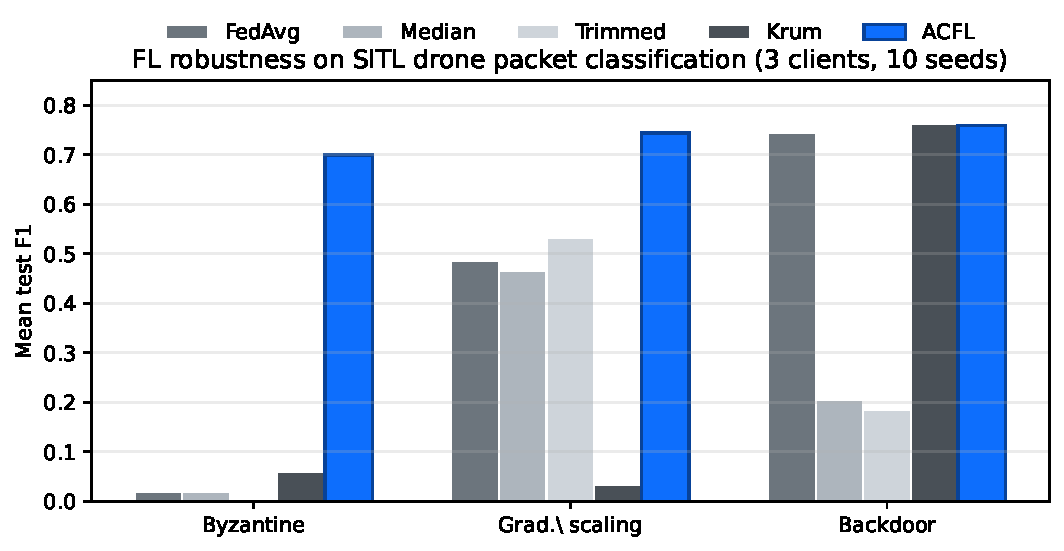
\includegraphics[width=\linewidth]{figures/fig_main_f1.pdf}
\caption{Mean test F1 across defenders and attacks on the SITL drone packet FL benchmark (3 clients, 12 rounds, 10 seeds). Only ACFL preserves utility under Byzantine attack; classical robust aggregators collapse or underperform FedAvg on gradient scaling and backdoor.}
\label{fig:main-f1}
\end{figure}

\begin{figure}[t]
\centering
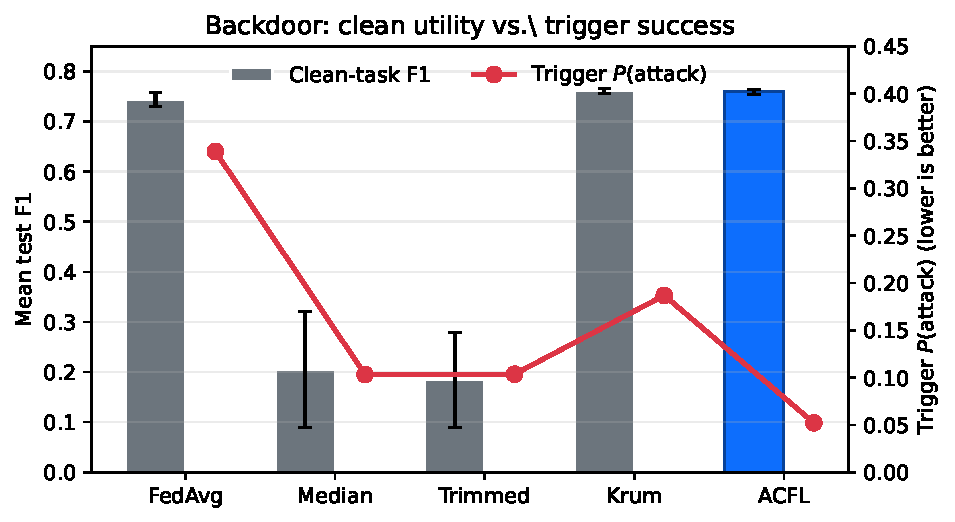
\includegraphics[width=\linewidth]{figures/fig_backdoor_dual.pdf}
\caption{Backdoor attack: clean-task F1 (bars, left axis) versus mean trigger $P(\text{attack})$ on counterfactual probes (line, right axis). Lower trigger probability indicates less successful backdoor activation. ACFL reduces trigger success relative to FedAvg and Krum while matching clean-task F1.}
\label{fig:backdoor-dual}
\end{figure}
.

%
% Companion tables: % Tables for the ACFL journal experiments section.
% Requires: \usepackage{booktabs}, \usepackage{multirow}
% Benchmark numbers: scripts/sync_manuscript_numbers.py -> tables_data.tex

% Auto-generated by scripts/compute_dataset_statistics.py — do not edit by hand.
\begin{table*}[!t]
\centering
\caption{SITL packet dataset characteristics (agent--mission layout).}
\label{tab:dataset}
\small
\resizebox{\textwidth}{!}{%
\begin{tabular}{@{}p{0.32\textwidth}p{0.64\textwidth}@{}}
\toprule
Quantity & Value \\
\midrule
Collection & ArduPilot SITL, 15.0$\times$ speedup; 8 waypoint, 7 GNSS, 5 benign missions \\
Topology & 10 agents $\times$ 2 missions (20 total); non-IID via cyclic agent assignment \\
Packet rows & 98,054 total; 6,627 attack (6.8\%) \\
Mission size & 2,635--6,891 packets/mission (median 4,719) \\
Flight duration & 108--286\,s/mission (median 202\,s) \\
Windowing & size 50, stride 25; temporal 80/20 train split on train missions \\
FL train windows & 1,458 raw (10.3\% attack); 1,601 after oversampling (25.0\% per agent with attacks) \\
Held-out eval & 1 mission/agent; 2,058 windows (8.3\% attack) \\
Eval (waypoint) & 4 agents, 697 windows, 5.7\% attack \\
Eval (gps) & 4 agents, 988 windows, 13.2\% attack \\
Eval (none) & 2 agents, 373 windows, 0.0\% attack \\
Features & SrcPort, DstPort, Length, MsgID, Protocol (binary \texttt{Label}) \\
Injection policy & 5 network injections/mission; GNSS spoof 25.0\,s; winds \{0, 6, 10\}\,m/s \\
\bottomrule
\end{tabular}%
}
\end{table*}

\begin{table}[t]
\centering
\caption{Per-mission packet statistics (held-out eval missions in bold).}
\label{tab:dataset-missions}
\scriptsize
\setlength{\tabcolsep}{3pt}
\begin{tabular}{@{}llrrrr@{}}
\toprule
Agent & Mission & Packets & Attack & Ratio & Duration (s) \\
\midrule
agent\_000 & d000 (waypoint) & 3259 & 129 & 4.0\% & 135 \\
agent\_001 & d001 (gps) & 6891 & 844 & 12.2\% & 286 \\
agent\_002 & d002 (none) & 3891 & 0 & 0.0\% & 165 \\
agent\_003 & d003 (waypoint) & 2635 & 120 & 4.6\% & 108 \\
agent\_004 & d004 (gps) & 6869 & 844 & 12.3\% & 285 \\
agent\_005 & d005 (none) & 4225 & 0 & 0.0\% & 180 \\
agent\_006 & d006 (waypoint) & 3179 & 125 & 3.9\% & 131 \\
agent\_007 & d007 (gps) & 6884 & 863 & 12.5\% & 284 \\
agent\_008 & d008 (none) & 5459 & 0 & 0.0\% & 234 \\
agent\_009 & d009 (waypoint) & 2725 & 117 & 4.3\% & 113 \\
agent\_000 & \textbf{d010 (waypoint)} & 3109 & 125 & 4.0\% & 128 \\
agent\_001 & \textbf{d011 (gps)} & 6876 & 838 & 12.2\% & 285 \\
agent\_002 & \textbf{d012 (waypoint)} & 6251 & 157 & 2.5\% & 264 \\
agent\_003 & \textbf{d013 (gps)} & 6889 & 852 & 12.4\% & 285 \\
agent\_004 & \textbf{d014 (waypoint)} & 4589 & 103 & 2.2\% & 193 \\
agent\_005 & \textbf{d015 (gps)} & 5584 & 688 & 12.3\% & 230 \\
agent\_006 & \textbf{d016 (none)} & 4706 & 0 & 0.0\% & 201 \\
agent\_007 & \textbf{d017 (waypoint)} & 3715 & 121 & 3.3\% & 156 \\
agent\_008 & \textbf{d018 (gps)} & 5586 & 701 & 12.5\% & 229 \\
agent\_009 & \textbf{d019 (none)} & 4732 & 0 & 0.0\% & 202 \\
\bottomrule
\end{tabular}
\end{table}

\begin{table}[t]
\centering
\caption{Per-agent federated learning window splits. Held-out eval mission shown in parentheses.}
\label{tab:dataset-agents}
\scriptsize
\setlength{\tabcolsep}{3pt}
\begin{tabular}{@{}lrrrrrr@{}}
\toprule
Agent & Train raw & Train bal. & Eval & Eval atk. & Held-out & Type \\
\midrule
agent\_000 & 103 (9.7\%) & 124 (25.0\%) & 122 & 9.0\% & (d010) & waypoint \\
agent\_001 & 219 (16.4\%) & 244 (25.0\%) & 273 & 12.8\% & (d011) & gps \\
agent\_002 & 123 (0.0\%) & 123 (0.0\%) & 248 & 4.8\% & (d012) & waypoint \\
agent\_003 & 83 (13.3\%) & 96 (25.0\%) & 273 & 13.2\% & (d013) & gps \\
agent\_004 & 218 (16.1\%) & 244 (25.0\%) & 181 & 5.0\% & (d014) & waypoint \\
agent\_005 & 134 (0.0\%) & 134 (0.0\%) & 221 & 13.1\% & (d015) & gps \\
agent\_006 & 100 (11.0\%) & 119 (25.2\%) & 186 & 0.0\% & (d016) & none \\
agent\_007 & 219 (16.9\%) & 243 (25.1\%) & 146 & 5.5\% & (d017) & waypoint \\
agent\_008 & 173 (0.0\%) & 173 (0.0\%) & 221 & 13.6\% & (d018) & gps \\
agent\_009 & 86 (11.6\%) & 101 (24.8\%) & 187 & 0.0\% & (d019) & none \\
\bottomrule
\end{tabular}
\end{table}

% Auto-generated by scripts/sync_manuscript_numbers.py — do not edit by hand.

\begin{table*}[t]
\centering
\caption{Mean test F1 ($\pm$ std) on the SITL drone packet FL benchmark (3 clients, 12 rounds, 10 seeds).}
\label{tab:main-f1}
\begin{tabular}{lccc}
\toprule
Defender & Byzantine & Grad.\ scaling & Backdoor \\
\midrule
FedAvg & 0.018 $\pm$ 0.030 & 0.486 $\pm$ 0.322 & 0.744 $\pm$ 0.014 \\
Coord.\ median & 0.019 $\pm$ 0.056 & 0.466 $\pm$ 0.172 & 0.205 $\pm$ 0.116 \\
Trimmed mean & 0.000 & 0.532 $\pm$ 0.043 & 0.184 $\pm$ 0.095 \\
Krum & 0.059 $\pm$ 0.069 & 0.032 $\pm$ 0.096 & \textbf{0.761 $\pm$ 0.005} \\
ACFL (full) & \textbf{0.699 $\pm$ 0.043} & \textbf{0.744 $\pm$ 0.011} & 0.759 $\pm$ 0.005 \\
\bottomrule
\end{tabular}
\end{table*}

\begin{table}[t]
\centering
\caption{Mean test F1 gap versus FedAvg (per-seed paired difference; 10 seeds).}
\label{tab:main-gap}
\small
\begin{tabular}{lccc}
\toprule
Defender & Byz.\ & Grad.\ & Backdoor \\
\midrule
Coord.\ median & $+0.000$ & $-0.021$ & $-0.539$ \\
Trimmed mean & $-0.018$ & $+0.045$ & $-0.560$ \\
Krum & $+0.041$ & $-0.454$ & $+0.017$ \\
ACFL (full) & \textbf{$+0.681$} & \textbf{$+0.257$} & $+0.015$ \\
\bottomrule
\end{tabular}
\end{table}

\begin{table}[t]
\centering
\caption{Backdoor: clean-task F1 and trigger $P(\text{attack})$ (lower is better; 10 seeds).}
\label{tab:backdoor-trigger}
\small
\begin{tabular}{lcc}
\toprule
Defender & $P(\text{attack})$ & Mean F1 \\
\midrule
FedAvg & 0.339 & 0.744 $\pm$ 0.014 \\
Coord.\ median & 0.103 & 0.205 $\pm$ 0.116 \\
Trimmed mean & 0.104 & 0.184 $\pm$ 0.095 \\
Krum & 0.187 & 0.761 $\pm$ 0.005 \\
ACFL (full) & \textbf{0.052} & 0.759 $\pm$ 0.005 \\
\bottomrule
\end{tabular}
\end{table}

\begin{table*}[t]
\centering
\caption{Layer ablation: mean test F1 ($\pm$ std) over 10 seeds (3 clients).}
\label{tab:ablation}
\small
\begin{tabular}{lccccc}
\toprule
Configuration & Byz. & Grad. & Backdoor & Label flip & Model repl. \\
\midrule
FedAvg & 0.015 $\pm$ 0.045 & 0.482 $\pm$ 0.280 & 0.744 $\pm$ 0.016 & 0.465 $\pm$ 0.199 & 0.000 \\
ACFL w/o L1 & 0.687 $\pm$ 0.047 & 0.728 $\pm$ 0.039 & 0.751 $\pm$ 0.006 & 0.609 $\pm$ 0.126 & 0.365 $\pm$ 0.184 \\
ACFL w/o L2 & \textbf{0.702 $\pm$ 0.046} & \textbf{0.747 $\pm$ 0.008} & \textbf{0.762 $\pm$ 0.007} & \textbf{0.749 $\pm$ 0.006} & 0.147 $\pm$ 0.021 \\
ACFL (full) & 0.680 $\pm$ 0.063 & 0.746 $\pm$ 0.013 & 0.758 $\pm$ 0.004 & 0.701 $\pm$ 0.025 & \textbf{0.473 $\pm$ 0.188} \\
\bottomrule
\end{tabular}
\end{table*}

\begin{table*}[t]
\centering
\caption{Layer ablation: malicious-client trust AUC over 10 seeds (FedAvg has no trust signal).}
\label{tab:ablation-trust}
\small
\begin{tabular}{lccccc}
\toprule
Configuration & Byz. & Grad. & Backdoor & Label flip & Model repl. \\
\midrule
FedAvg & --- & --- & --- & --- & --- \\
ACFL w/o L1 & 0.500 & 0.500 & 0.500 & 0.500 & 0.500 \\
ACFL w/o L2 & 1.000 & 1.000 & 0.522 & 0.595 & 0.999 \\
ACFL (full) & 1.000 & 0.996 & 0.563 & 0.551 & 0.969 \\
\bottomrule
\end{tabular}
\end{table*}

\begin{table}[t]
\centering
\caption{Threat-model gap attacks (3 clients, 10 seeds): mean test F1 ($\pm$ std).}
\label{tab:threat-gaps}
\small
\begin{tabular}{lccr}
\toprule
Defender & Label flip & Model repl.\ & $\Delta$ LF \\
\midrule
FedAvg & 0.465 $\pm$ 0.199 & 0.000 & --- \\
Coord.\ median & 0.111 $\pm$ 0.039 & 0.000 & $-0.354$ \\
Trimmed mean & 0.123 $\pm$ 0.064 & 0.000 & $-0.342$ \\
Krum & 0.540 $\pm$ 0.174 & 0.000 & $+0.075$ \\
ACFL (full) & \textbf{0.701 $\pm$ 0.025} & \textbf{0.473 $\pm$ 0.188} & \textbf{$+0.236$} \\
\bottomrule
\end{tabular}
\end{table}

\begin{table}[t]
\centering
\caption{Backdoor gating ablation: legacy min-blend vs.\ probe-aware soft cap (3 seeds).}
\label{tab:probe-cap-ablation}
\small
\begin{tabular}{lcccc}
\toprule
Seed & Legacy F1 & Probe F1 & Legacy $P(\text{atk})$ & Probe $P(\text{atk})$ \\
\midrule
42 & 0.760 & 0.753 & 0.165 & 0.339 \\
43 & 0.761 & 0.768 & 0.246 & 0.271 \\
44 & 0.766 & 0.757 & 0.187 & 0.180 \\
\midrule
Mean & 0.762 & 0.760 & 0.199 & 0.263 \\
\bottomrule
\end{tabular}
\end{table}

\begin{table}[t]
\centering
\caption{Backdoor scrub ablation (10 seeds): shortlist-veto only vs.\ veto + post-aggregation trigger scrub at $n{=}3$ (journal) and $n{=}5$ (20\% malicious, min.\ quorum 4).}
\label{tab:scrub-ablation}
\small
\begin{tabular}{llcc}
\toprule
Scale & Variant & Mean F1 & $P(\text{attack})$ \\
\midrule
\multirow{3}{*}{$n{=}3$}
  & Veto only & 0.763 $\pm$ 0.006 & 0.176 $\pm$ 0.045 \\
  & Veto + scrub & 0.761 $\pm$ 0.004 & \textbf{0.046 $\pm$ 0.015} \\
  & Scrub $-$ veto & $-0.001$ & $-0.130$ \\
\midrule
\multirow{3}{*}{$n{=}5$}
  & Veto only & 0.758 $\pm$ 0.011 & 0.174 $\pm$ 0.037 \\
  & Veto + scrub & 0.761 $\pm$ 0.005 & \textbf{0.064 $\pm$ 0.029} \\
  & Scrub $-$ veto & $+0.004$ & $-0.111$ \\
\bottomrule
\end{tabular}
\end{table}

\begin{table}[t]
\centering
\caption{Five-client benchmark (20\% malicious, 10 seeds): Byzantine and gradient-scaling mean test F1 ($\pm$ std).}
\label{tab:5client-byz-grad}
\small
\begin{tabular}{lccr}
\toprule
Defender & Byzantine & Grad.\ scaling & $\Delta$ F1 (Byz.) \\
\midrule
FedAvg & 0.016 $\pm$ 0.040 & 0.687 $\pm$ 0.079 & --- \\
Coord.\ median & 0.000 & 0.075 $\pm$ 0.225 & $-0.016$ \\
Trimmed mean & 0.056 $\pm$ 0.123 & 0.145 $\pm$ 0.291 & $+0.040$ \\
Krum & 0.680 $\pm$ 0.227 & 0.439 $\pm$ 0.362 & $+0.664$ \\
ACFL (full) & \textbf{0.739 $\pm$ 0.020} & \textbf{0.750 $\pm$ 0.010} & \textbf{$+0.723$} \\
\bottomrule
\end{tabular}
\end{table}

\begin{table}[t]
\centering
\caption{Five-client backdoor benchmark (5 clients, min.\ 4/round, 20\% malicious, 10 seeds): clean F1 and trigger $P(\text{attack})$.}
\label{tab:5client-backdoor}
\small
\begin{tabular}{lccr}
\toprule
Defender & Mean F1 & $P(\text{attack})$ & $\Delta$ F1 \\
\midrule
FedAvg & 0.651 $\pm$ 0.197 & 0.386 & --- \\
Coord.\ median & 0.711 $\pm$ 0.100 & 0.262 & $+0.060$ \\
Trimmed mean & 0.672 $\pm$ 0.137 & 0.233 & $+0.021$ \\
Krum & 0.760 $\pm$ 0.005 & 0.177 & $+0.109$ \\
ACFL (full) & \textbf{0.760 $\pm$ 0.003} & \textbf{0.059} & \textbf{$+0.109$} \\
\bottomrule
\end{tabular}
\end{table}

\begin{table}[t]
\centering
\caption{Five-client label-flip benchmark (50\% local flip, 20\% malicious, 10 seeds): mean test F1 ($\pm$ std).}
\label{tab:5client-label-flip}
\small
\begin{tabular}{lcr}
\toprule
Defender & Mean F1 & $\Delta$ vs FedAvg \\
\midrule
FedAvg & 0.618 $\pm$ 0.227 & --- \\
Coord.\ median & 0.531 $\pm$ 0.227 & $-0.087$ \\
Trimmed mean & 0.566 $\pm$ 0.189 & $-0.052$ \\
Krum & 0.746 $\pm$ 0.016 & $+0.129$ \\
ACFL (full) & \textbf{0.751 $\pm$ 0.011} & \textbf{$+0.133$} \\
\bottomrule
\end{tabular}
\end{table}

\begin{table}[t]
\centering
\caption{Five-client model-replacement benchmark ($\alpha{=}10$ anti-direction, 20\% malicious, minimum quorum four for ACFL/Krum, 10 seeds): mean test F1 ($\pm$ std).}
\label{tab:5client-model-replacement}
\small
\begin{tabular}{lcr}
\toprule
Defender & Mean F1 & $\Delta$ vs FedAvg \\
\midrule
FedAvg & 0.042 $\pm$ 0.064 & --- \\
Coord.\ median & 0.014 $\pm$ 0.042 & $-0.028$ \\
Trimmed mean & 0.014 $\pm$ 0.042 & $-0.028$ \\
Krum & 0.286 $\pm$ 0.345 & $+0.244$ \\
ACFL (full) & \textbf{0.607 $\pm$ 0.147} & \textbf{$+0.566$} \\
\bottomrule
\end{tabular}
\\[0.5em]
{\footnotesize ACFL (full): Layer~1 probe trust in aggregation, attack-scoped hard norm rejection (withheld if too few clients remain), trust AUC 0.995. FedAvg/median/trimmed rows from minimum-quorum-three extension; ACFL and Krum regenerated at quorum four.}
\end{table}

\begin{table}[t]
\centering
\caption{Layer~3 spoofing detection on held-out SITL packet missions (ACFL checkpoint, probe-calibrated $P(\text{attack})$).}
\label{tab:layer3}
\small
\begin{tabular}{lcc}
\toprule
Metric & Value & Notes \\
\midrule
Aggregate AUROC & 0.968 & 10 agents, held-out missions \\
Aggregate F1 & 0.916 & threshold tuned on eval windows \\
\bottomrule
\end{tabular}
\end{table}

% BEGIN layer3-operational-table
\begin{table}[t]
\centering
\caption{Layer~3 operational metrics on held-out SITL missions (time-to-detect, false alarms, inference latency).}
\label{tab:layer3-operational}
\scriptsize
\setlength{\tabcolsep}{3pt}
\begin{tabular}{@{}p{0.36\columnwidth}p{0.30\columnwidth}p{0.28\columnwidth}@{}}
\toprule
Metric & Value & Notes \\
\midrule
Mean time-to-detect & 0.78\,s (0.8 win.) & det.\ rate 1.00 \\
False-alarm rate & 0.005 & 10 FP / 1888 benign \\
False alarms/hour & 8.9 & median 8.9 \\
Inference latency & 0.52\,ms & p95 0.70\,ms \\
gps missions & TTD 1.03\,s & FA 0.007 \\
none missions & TTD N/A & FA 0.003 \\
waypoint missions & TTD 0.52\,s & FA 0.005 \\
\bottomrule
\end{tabular}
\end{table}
% END layer3-operational-table

\begin{table*}[t]
\centering
\caption{Combined network+learning Layer~3 validation: poisoned FL checkpoint then Layer~3 on held-out waypoint/GNSS missions (10 seeds, FedAvg vs ACFL).}
\label{tab:combined-layer3}
\small
\begin{tabular}{lccr}
\toprule
Learning attack & FedAvg AUROC & ACFL AUROC & $\Delta$ \\
\midrule
Benign (no FL poison) & 0.984 $\pm$ 0.008 & 0.986 $\pm$ 0.009 & $+0.002$ \\
Gradient scaling & 0.883 $\pm$ 0.192 & 0.963 $\pm$ 0.013 & $+0.080$ \\
Byzantine & 0.538 $\pm$ 0.201 & \textbf{0.872 $\pm$ 0.106} & \textbf{$+0.334$} \\
Backdoor & 0.985 $\pm$ 0.007 & 0.985 $\pm$ 0.008 & $+0.000$ \\
Label flip & 0.830 $\pm$ 0.124 & 0.901 $\pm$ 0.054 & $+0.071$ \\
Model repl. & 0.419 $\pm$ 0.165 & \textbf{0.692 $\pm$ 0.267} & \textbf{$+0.273$} \\
\bottomrule
\end{tabular}
\\[0.5em]
{\footnotesize Shared FedAvg/ACFL-full \emph{attack} cells use the same 3-client checkpoints as Table~\ref{tab:full-stack} (ablation for Byz./grad./backdoor; threat-gap for label flip and model replacement), so Layer~3 AUROC means match bit-for-bit. The benign row is a matched 12-round \texttt{config\_classification\_drone} control (seeds 42--51), not the legacy 5-round \texttt{classification\_benign} checkpoint. FedAvg gradient-scaling AUROC variance includes two seeds whose poisoned checkpoints emit non-finite detector scores (sanitized to chance-level AUROC~$0.5$).}
\end{table*}

\begin{table*}[t]
\centering
\caption{Full-stack validation: Layer~1 trust AUC, Layer~2 clean F1, and Layer~3 spoofing AUROC on the \emph{same} checkpoint per configuration (10 seeds, $\pm$ std over seeds). FedAvg has no Layer~1 trust signal.}
\label{tab:full-stack}
\small
\begin{tabular}{llccc}
\toprule
Attack & Stack & L1 trust AUC & L2 F1 & L3 AUROC \\
\midrule
\multirow{4}{*}{Byzantine} & FedAvg (no L1/L2) & --- & 0.017 $\pm$ 0.047 & 0.538 $\pm$ 0.201 \\
 & Layer~1 only & 1.000 & \textbf{0.701 $\pm$ 0.048} & \textbf{0.898 $\pm$ 0.072} \\
 & Layer~2 only & 0.500 & 0.683 $\pm$ 0.047 & 0.881 $\pm$ 0.091 \\
 & L1+L2+L3 (full) & \textbf{1.000} & 0.674 $\pm$ 0.064 & 0.872 $\pm$ 0.106 \\
\midrule
\multirow{4}{*}{Grad.\ scaling} & FedAvg (no L1/L2) & --- & 0.482 $\pm$ 0.280 & 0.883 $\pm$ 0.192 \\
 & Layer~1 only & 1.000 & \textbf{0.747 $\pm$ 0.008} & \textbf{0.965 $\pm$ 0.013} \\
 & Layer~2 only & 0.500 & 0.728 $\pm$ 0.039 & 0.963 $\pm$ 0.013 \\
 & L1+L2+L3 (full) & \textbf{0.996 $\pm$ 0.008} & 0.746 $\pm$ 0.013 & 0.963 $\pm$ 0.013 \\
\midrule
\multirow{4}{*}{Backdoor} & FedAvg (no L1/L2) & --- & 0.744 $\pm$ 0.016 & 0.985 $\pm$ 0.007 \\
 & Layer~1 only & 0.568 $\pm$ 0.060 & 0.757 $\pm$ 0.010 & \textbf{0.985 $\pm$ 0.008} \\
 & Layer~2 only & 0.500 & 0.749 $\pm$ 0.005 & 0.982 $\pm$ 0.010 \\
 & L1+L2+L3 (full) & 0.563 $\pm$ 0.117 & \textbf{0.758 $\pm$ 0.004} & 0.985 $\pm$ 0.008 \\
\midrule
\multirow{4}{*}{Label flip} & FedAvg (no L1/L2) & --- & 0.465 $\pm$ 0.199 & 0.830 $\pm$ 0.124 \\
 & Layer~1 only & 0.595 $\pm$ 0.048 & \textbf{0.749 $\pm$ 0.006} & \textbf{0.957 $\pm$ 0.020} \\
 & Layer~2 only & 0.500 & 0.609 $\pm$ 0.126 & 0.757 $\pm$ 0.222 \\
 & L1+L2+L3 (full) & 0.551 $\pm$ 0.034 & 0.701 $\pm$ 0.025 & 0.901 $\pm$ 0.054 \\
\midrule
\multirow{4}{*}{Model repl.} & FedAvg (no L1/L2) & --- & 0.000 & 0.419 $\pm$ 0.165 \\
 & Layer~1 only & 0.999 $\pm$ 0.002 & 0.147 $\pm$ 0.021 & 0.225 $\pm$ 0.131 \\
 & Layer~2 only & 0.500 & 0.365 $\pm$ 0.184 & 0.648 $\pm$ 0.333 \\
 & L1+L2+L3 (full) & 0.969 $\pm$ 0.024 & \textbf{0.473 $\pm$ 0.188} & \textbf{0.692 $\pm$ 0.267} \\
\bottomrule
\end{tabular}
\\[0.5em]
{\footnotesize Bold marks the best mean Layer~2 F1 and Layer~3 AUROC within each attack block. All rows use 3-client checkpoints (ablation for Byz./grad./backdoor; threat-gap for label flip and model replacement). FedAvg/full Layer~3 AUROC means match Table~\ref{tab:combined-layer3} bit-for-bit on shared attacks.}
\end{table*}

\begin{table*}[t]
\centering
\caption{Full-stack Layer~3 operational metrics on held-out SITL missions (FedAvg, classical robust aggregators, and ACFL-full; 10 seeds; per-checkpoint F1-tuned threshold). FedAvg/ACFL-full poisoned rows reuse Table~\ref{tab:full-stack} checkpoints; classical rows use the matching journal/threat 3-client runs; benign is the matched 12-round drone control (FedAvg and ACFL-full only).}
\label{tab:full-stack-ops}
\scriptsize
\setlength{\tabcolsep}{4pt}
\begin{tabular}{llcccc}
\toprule
Attack & Defender & TTD (s) & Det.\ rate & FA/hr & Latency mean/p95 (ms) \\
\midrule
\multirow{2}{*}{Benign} & FedAvg & 1.00 $\pm$ 0.30 & 1.000 & 6.2 $\pm$ 6.0 & 1.59/6.20 \\
 & ACFL (full) & 0.91 $\pm$ 0.17 & 1.000 & \textbf{4.4 $\pm$ 4.7} & 1.59/6.20 \\
\midrule
\multirow{5}{*}{Byzantine} & FedAvg & 2.09 $\pm$ 3.33 & 0.838 $\pm$ 0.145 & 1472.4 $\pm$ 1643.2 & 1.59/6.20 \\
 & Coord.\ median & 1.37 $\pm$ 0.78 & 0.350 $\pm$ 0.099 & 70.3 $\pm$ 145.8 & 1.59/6.20 \\
 & Trimmed mean & 0.99 $\pm$ 0.59 & 0.475 $\pm$ 0.281 & 665.4 $\pm$ 1402.9 & 1.59/6.20 \\
 & Krum & 1.82 $\pm$ 4.18 & 0.900 $\pm$ 0.184 & 2270.0 $\pm$ 1570.2 & 1.59/6.20 \\
 & ACFL (full) & 1.50 $\pm$ 1.18 & 0.912 $\pm$ 0.103 & \textbf{32.0 $\pm$ 79.8} & 1.59/6.20 \\
\midrule
\multirow{5}{*}{Grad.\ scaling} & FedAvg & 0.84 $\pm$ 0.58 & 0.938 $\pm$ 0.121 & 677.0 $\pm$ 1396.9 & 1.59/6.20 \\
 & Coord.\ median & 1.91 $\pm$ 1.11 & 0.875 $\pm$ 0.102 & 843.5 $\pm$ 1171.6 & 1.59/6.20 \\
 & Trimmed mean & 2.78 $\pm$ 3.57 & 0.863 $\pm$ 0.181 & 1022.3 $\pm$ 880.3 & 1.59/6.20 \\
 & Krum & 0.09 $\pm$ 0.29 & 1.000 & 2996.3 $\pm$ 1046.5 & 1.59/6.20 \\
 & ACFL (full) & 1.14 $\pm$ 0.63 & 1.000 & \textbf{1.8 $\pm$ 3.8} & 1.59/6.20 \\
\midrule
\multirow{5}{*}{Backdoor} & FedAvg & 0.74 $\pm$ 0.25 & 1.000 & 8.0 $\pm$ 2.8 & 1.59/6.20 \\
 & Coord.\ median & 1.26 $\pm$ 1.61 & 0.875 $\pm$ 0.144 & 2500.0 $\pm$ 872.0 & 1.59/6.20 \\
 & Trimmed mean & 0.94 $\pm$ 1.55 & 0.887 $\pm$ 0.150 & 2661.9 $\pm$ 859.1 & 1.59/6.20 \\
 & Krum & 0.79 $\pm$ 0.14 & 1.000 & 7.1 $\pm$ 8.2 & 1.59/6.20 \\
 & ACFL (full) & 0.88 $\pm$ 0.25 & 1.000 & \textbf{3.6 $\pm$ 4.6} & 1.59/6.20 \\
\midrule
\multirow{5}{*}{Label flip} & FedAvg & 2.65 $\pm$ 1.95 & 0.838 $\pm$ 0.205 & \textbf{2.7 $\pm$ 8.4} & 1.59/6.20 \\
 & Coord.\ median & 0.53 $\pm$ 1.35 & 0.938 $\pm$ 0.135 & 2992.8 $\pm$ 705.1 & 1.59/6.20 \\
 & Trimmed mean & 0.84 $\pm$ 1.77 & 0.950 $\pm$ 0.105 & 2992.8 $\pm$ 705.1 & 1.59/6.20 \\
 & Krum & 4.60 $\pm$ 10.17 & 0.875 $\pm$ 0.167 & 521.4 $\pm$ 1124.2 & 1.59/6.20 \\
 & ACFL (full) & 1.83 $\pm$ 1.80 & 0.963 $\pm$ 0.084 & 36.7 $\pm$ 103.7 & 1.59/6.20 \\
\midrule
\multirow{5}{*}{Model repl.} & FedAvg & 0.00 & 1.000 & 3327.2 & 1.59/6.20 \\
 & Coord.\ median & 0.00 & 1.000 & 3327.2 & 1.59/6.20 \\
 & Trimmed mean & 0.00 & 1.000 & 3327.2 & 1.59/6.20 \\
 & Krum & 0.00 & 1.000 & 3327.2 & 1.59/6.20 \\
 & ACFL (full) & 2.29 $\pm$ 1.89 & 0.950 $\pm$ 0.087 & \textbf{816.6 $\pm$ 1392.4} & 1.59/6.20 \\
\bottomrule
\end{tabular}
\\[0.5em]
{\footnotesize TTD $=$ mean time-to-detect from labeled attack onset; det.\ rate $=$ fraction of attack onsets detected; FA/hr $=$ false alarms per operating hour on benign (no-network-attack) missions; latency $=$ shared mean/p95 CPU inference time per packet window, measured sequentially over 10 repeats on the common TinyPacketCNN + spoofing-detector path. FA/hr is a duration-normalized \emph{rate} (false positives divided by each mission's true span, then scaled to one hour), not an hour-long simulation: eval missions run $\approx$2--5\,min, so the extrapolation factor is $\approx$12--28$\times$. Bold marks the lowest mean FA/hr within each attack. Collapsed checkpoints (e.g.\ FedAvg under model replacement) saturate detections by flagging nearly every benign window (det.\ rate $\approx 1$ with FA/hr in the thousands). Classical aggregators have no matched benign control under the 12-round drone protocol.}
\end{table*}

\begin{table}[t]
\centering
\caption{Server-side per-round aggregation overhead (CPU, single thread; 3 clients, drone TinyPacketCNN; mean $\pm$ std over 50 rounds). Layers~1--2 run once per FL round at training time; this is distinct from the inference-time Layer~3 latency in Table~\ref{tab:full-stack-ops}.}
\label{tab:aggregation-overhead}
\small
\begin{tabular}{lcc}
\toprule
Aggregator & Per-round (ms) & $\times$ FedAvg \\
\midrule
FedAvg & 3.75 $\pm$ 0.26 & 1.0$\times$ \\
Coord.\ median & 3.69 $\pm$ 0.18 & 1.0$\times$ \\
Trimmed mean & 3.84 $\pm$ 0.23 & 1.0$\times$ \\
Krum & 3.21 $\pm$ 0.27 & 0.9$\times$ \\
ACFL (L1+L2) & 22.31 $\pm$ 1.43 & 6.0$\times$ \\
\bottomrule
\end{tabular}
\\[0.5em]
{\footnotesize Overhead is a once-per-round \emph{training} cost, not a per-window inference cost; over a 12-round run the extra wall-clock is sub-second in absolute terms. With full probes, Layer~1 is 21.8\,ms and Layer~2 is 8.9\,ms; batched probe evaluation cuts the prior $\approx$58\,ms stack to 24.7\,ms; the drone path (16 windows/scenario + attack-scoped subsets) is 22.3\,ms. Client updates are weight-scaled perturbations of a real drone checkpoint so probe forward passes are realistic. Production ACFL uses the drone probe path (Table~\ref{tab:probe-config-ablation}).}
\end{table}

\begin{table}[t]
\centering
\caption{Layer~1 probe-config ablation on ACFL-full (3 clients, 12 rounds, 10 seeds): full probe set (all scenarios $\times$ 48 windows) vs.\ the drone production path (16 windows/scenario + attack-scoped subsets). $\Delta$ is drone$-$full (paired).}
\label{tab:probe-config-ablation}
\small
\begin{tabular}{lcccc}
\toprule
Attack & Full F1 & Drone F1 & $\Delta$F1 & $\Delta$ trust AUC \\
\midrule
Byzantine & 0.690 $\pm$ 0.039 & 0.702 $\pm$ 0.035 & $+0.011$ & $+0.008$ \\
Backdoor & 0.762 $\pm$ 0.004 & 0.738 $\pm$ 0.013 & $-0.024$ & $+0.016$ \\
Label flip & 0.749 $\pm$ 0.010 & 0.750 $\pm$ 0.014 & $+0.001$ & $-0.059$ \\
\bottomrule
\end{tabular}
\\[0.5em]
{\footnotesize Byzantine and label-flip F1 are essentially unchanged under the faster path. Backdoor shows a modest clean-F1 cost ($\approx$0.024) while trust AUC is slightly higher; we retain the drone path as the production default and note the backdoor tradeoff.}
\end{table}

\begin{table*}[t]
\centering
\caption{Attack-intensity sensitivity: mean test F1 ($\pm$ std; 3 clients, 12 rounds, 5 seeds). One knob varies per attack; $^*$ marks the manuscript primary setting. $\Delta$ is ACFL$-$FedAvg (paired).}
\label{tab:attack-intensity}
\small
\setlength{\tabcolsep}{3.5pt}
\begin{tabular}{llcccccc}
\toprule
Attack & Intensity & FedAvg & Coord.\ med. & Trimmed & Krum & ACFL & $\Delta$ \\
\midrule
Backdoor & poison=0.15 & 0.745 $\pm$ 0.012 & 0.117 $\pm$ 0.039 & 0.101 $\pm$ 0.012 & 0.711 $\pm$ 0.085 & \textbf{0.747 $\pm$ 0.007} & $+0.001$ \\
 & poison=0.35$^*$ & 0.744 $\pm$ 0.033 & 0.113 $\pm$ 0.028 & 0.100 $\pm$ 0.020 & \textbf{0.760 $\pm$ 0.011} & 0.748 $\pm$ 0.008 & $+0.004$ \\
 & poison=0.55 & 0.755 $\pm$ 0.016 & 0.210 $\pm$ 0.220 & 0.094 $\pm$ 0.020 & \textbf{0.761 $\pm$ 0.006} & 0.743 $\pm$ 0.010 & $-0.012$ \\
Byzantine & $\sigma$=0.25 & 0.000 & 0.042 $\pm$ 0.064 & 0.039 $\pm$ 0.021 & 0.097 $\pm$ 0.107 & \textbf{0.742 $\pm$ 0.019} & $+0.742$ \\
 & $\sigma$=0.5 & 0.126 $\pm$ 0.253 & 0.000 & 0.000 & 0.000 & \textbf{0.734 $\pm$ 0.020} & $+0.608$ \\
 & $\sigma$=1$^*$ & 0.021 $\pm$ 0.042 & 0.000 & 0.000 & 0.028 $\pm$ 0.056 & \textbf{0.701 $\pm$ 0.017} & $+0.680$ \\
 & $\sigma$=2 & 0.028 $\pm$ 0.050 & 0.000 & 0.000 & 0.143 $\pm$ 0.159 & \textbf{0.542 $\pm$ 0.139} & $+0.514$ \\
Grad.\ scaling & scale=2 & \textbf{0.757 $\pm$ 0.008} & 0.200 $\pm$ 0.061 & 0.204 $\pm$ 0.077 & 0.667 $\pm$ 0.106 & 0.753 $\pm$ 0.015 & $-0.005$ \\
 & scale=5 & 0.739 $\pm$ 0.011 & 0.414 $\pm$ 0.074 & 0.384 $\pm$ 0.045 & 0.681 $\pm$ 0.060 & \textbf{0.745 $\pm$ 0.015} & $+0.006$ \\
 & scale=10$^*$ & 0.279 $\pm$ 0.342 & 0.202 $\pm$ 0.247 & 0.294 $\pm$ 0.241 & 0.000 & \textbf{0.751 $\pm$ 0.012} & $+0.472$ \\
 & scale=20 & 0.270 $\pm$ 0.333 & 0.212 $\pm$ 0.260 & 0.206 $\pm$ 0.252 & 0.000 & \textbf{0.754 $\pm$ 0.011} & $+0.483$ \\
Label flip & flip=0.25 & 0.739 $\pm$ 0.012 & 0.107 $\pm$ 0.014 & 0.106 $\pm$ 0.024 & 0.584 $\pm$ 0.240 & \textbf{0.753 $\pm$ 0.009} & $+0.014$ \\
 & flip=0.5$^*$ & 0.573 $\pm$ 0.058 & 0.086 $\pm$ 0.003 & 0.084 $\pm$ 0.003 & 0.460 $\pm$ 0.190 & \textbf{0.752 $\pm$ 0.004} & $+0.178$ \\
 & flip=0.75 & 0.276 $\pm$ 0.169 & 0.077 $\pm$ 0.004 & 0.091 $\pm$ 0.025 & 0.359 $\pm$ 0.180 & \textbf{0.754 $\pm$ 0.009} & $+0.477$ \\
Model repl. & $\alpha$=5 & 0.083 $\pm$ 0.068 & 0.000 & 0.000 & 0.111 $\pm$ 0.056 & \textbf{0.181 $\pm$ 0.052} & $+0.098$ \\
 & $\alpha$=10$^*$ & 0.000 & 0.000 & 0.000 & 0.000 & \textbf{0.353 $\pm$ 0.208} & $+0.353$ \\
 & $\alpha$=20 & 0.000 & 0.000 & 0.000 & 0.000 & \textbf{0.506 $\pm$ 0.221} & $+0.506$ \\
\bottomrule
\end{tabular}
\\[0.5em]
{\footnotesize Primary settings match Section~\ref{sec:exp-attacks}. Coordinate median and trimmed mean often sacrifice clean utility; Krum is seed-volatile on gradient scaling and weak under label flip. ACFL remains the most stable defender as intensity increases. Backdoor trigger probabilities are in Table~\ref{tab:attack-intensity-backdoor}.}
\end{table*}

\begin{table}[t]
\centering
\caption{Backdoor intensity sweep: mean trigger $P(\text{attack})$ (5 seeds; lower is better).}
\label{tab:attack-intensity-backdoor}
\small
\begin{tabular}{lcccc}
\toprule
Poison frac. & FedAvg & Coord.\ med. & Krum & ACFL \\
\midrule
0.15 & 0.323 & 0.141 & 0.259 & \textbf{0.017} \\
0.35$^*$ & 0.333 & 0.092 & 0.189 & \textbf{0.016} \\
0.55 & 0.324 & 0.085 & 0.189 & \textbf{0.019} \\
\bottomrule
\end{tabular}
\\[0.5em]
{\footnotesize ACFL keeps trigger activation near 0.02 across poison fractions while matching clean-task F1 (Table~\ref{tab:attack-intensity}).}
\end{table}

\begin{table*}[t]
\centering
\caption{Layer~1 isolation across the attack-intensity sweep (5 seeds): ACFL with Layer~2 disabled (\texttt{acfl\_l1\_only}) versus the full stack. $\Delta$F1 is L1-only$-$full (matched intensity/seed means). $^*$ marks the primary setting.}
\label{tab:attack-intensity-l1}
\small
\begin{tabular}{llcccc}
\toprule
Attack & Intensity & L1-only F1 & Full F1 & $\Delta$F1 & L1 / full trust AUC \\
\midrule
Backdoor & poison=0.15 & 0.741 $\pm$ 0.012 & 0.747 $\pm$ 0.007 & $-0.006$ & 0.604 / 0.525 \\
 & poison=0.35$^*$ & 0.745 $\pm$ 0.011 & 0.748 $\pm$ 0.008 & $-0.003$ & 0.682 / 0.664 \\
 & poison=0.55 & 0.746 $\pm$ 0.011 & 0.743 $\pm$ 0.010 & $+0.004$ & 0.622 / 0.578 \\
Byzantine & $\sigma$=0.25 & 0.703 $\pm$ 0.081 & 0.742 $\pm$ 0.019 & $-0.039$ & 0.989 / 0.996 \\
 & $\sigma$=0.5 & 0.738 $\pm$ 0.026 & 0.734 $\pm$ 0.020 & $+0.003$ & 0.997 / 0.996 \\
 & $\sigma$=1$^*$ & 0.715 $\pm$ 0.027 & 0.701 $\pm$ 0.017 & $+0.014$ & 0.999 / 0.996 \\
 & $\sigma$=2 & 0.600 $\pm$ 0.118 & 0.542 $\pm$ 0.139 & $+0.058$ & 1.000 / 0.996 \\
Grad.\ scaling & scale=2 & 0.768 $\pm$ 0.007 & 0.753 $\pm$ 0.015 & $+0.016$ & 0.793 / 0.853 \\
 & scale=5 & 0.743 $\pm$ 0.009 & 0.745 $\pm$ 0.015 & $-0.002$ & 0.986 / 0.975 \\
 & scale=10$^*$ & 0.743 $\pm$ 0.020 & 0.751 $\pm$ 0.012 & $-0.009$ & 0.988 / 0.994 \\
 & scale=20 & 0.758 $\pm$ 0.003 & 0.754 $\pm$ 0.011 & $+0.004$ & 0.971 / 1.000 \\
Label flip & flip=0.25 & 0.758 $\pm$ 0.004 & 0.753 $\pm$ 0.009 & $+0.004$ & 0.590 / 0.530 \\
 & flip=0.5$^*$ & 0.744 $\pm$ 0.005 & 0.752 $\pm$ 0.004 & $-0.008$ & 0.505 / 0.577 \\
 & flip=0.75 & 0.755 $\pm$ 0.011 & 0.754 $\pm$ 0.009 & $+0.001$ & 0.558 / 0.542 \\
Model repl. & $\alpha$=5 & 0.140 $\pm$ 0.000 & 0.181 $\pm$ 0.052 & $-0.041$ & 1.000 / 0.926 \\
 & $\alpha$=10$^*$ & 0.163 $\pm$ 0.041 & 0.353 $\pm$ 0.208 & $-0.190$ & 1.000 / 1.000 \\
 & $\alpha$=20 & 0.365 $\pm$ 0.188 & 0.506 $\pm$ 0.221 & $-0.141$ & 1.000 / 0.999 \\
\bottomrule
\end{tabular}
\\[0.5em]
{\footnotesize On gradient scaling, Byzantine, backdoor, and label flip, L1-only tracks the full stack within $\approx$0.06 F1 across intensities. Model replacement is the clear exception: disabling Layer~2 costs $\approx$0.14--0.19 F1 at $\alpha{\ge}10$, confirming that hard-rejection/aggregation (Layer~2) is load-bearing for that threat while Layer~1 still attributes the adversary (trust AUC $\approx 1$).}
\end{table*}

\begin{table*}[t]
\centering
\caption{Layer~2 isolation across the attack-intensity sweep (5 seeds): ACFL with Layer~1 disabled (\texttt{acfl\_l2\_only}) versus the full stack. $\Delta$F1 is L2-only$-$full (matched intensity/seed means). $^*$ marks the primary setting.}
\label{tab:attack-intensity-l2}
\small
\begin{tabular}{llcccc}
\toprule
Attack & Intensity & L2-only F1 & Full F1 & $\Delta$F1 & L2 / full trust AUC \\
\midrule
Backdoor & poison=0.15 & 0.760 $\pm$ 0.006 & 0.747 $\pm$ 0.007 & $+0.014$ & 0.500 / 0.525 \\
 & poison=0.35$^*$ & 0.758 $\pm$ 0.009 & 0.748 $\pm$ 0.008 & $+0.010$ & 0.500 / 0.664 \\
 & poison=0.55 & 0.761 $\pm$ 0.004 & 0.743 $\pm$ 0.010 & $+0.019$ & 0.500 / 0.578 \\
Byzantine & $\sigma$=0.25 & 0.733 $\pm$ 0.017 & 0.742 $\pm$ 0.019 & $-0.009$ & 0.500 / 0.996 \\
 & $\sigma$=0.5 & 0.731 $\pm$ 0.024 & 0.734 $\pm$ 0.020 & $-0.004$ & 0.500 / 0.996 \\
 & $\sigma$=1$^*$ & 0.703 $\pm$ 0.029 & 0.701 $\pm$ 0.017 & $+0.002$ & 0.500 / 0.996 \\
 & $\sigma$=2 & 0.496 $\pm$ 0.200 & 0.542 $\pm$ 0.139 & $-0.046$ & 0.500 / 0.996 \\
Grad.\ scaling & scale=2 & 0.757 $\pm$ 0.009 & 0.753 $\pm$ 0.015 & $+0.005$ & 0.500 / 0.853 \\
 & scale=5 & 0.738 $\pm$ 0.009 & 0.745 $\pm$ 0.015 & $-0.007$ & 0.500 / 0.975 \\
 & scale=10$^*$ & 0.742 $\pm$ 0.009 & 0.751 $\pm$ 0.012 & $-0.010$ & 0.500 / 0.994 \\
 & scale=20 & 0.755 $\pm$ 0.011 & 0.754 $\pm$ 0.011 & $+0.001$ & 0.500 / 1.000 \\
Label flip & flip=0.25 & 0.760 $\pm$ 0.004 & 0.753 $\pm$ 0.009 & $+0.007$ & 0.500 / 0.530 \\
 & flip=0.5$^*$ & 0.689 $\pm$ 0.070 & 0.752 $\pm$ 0.004 & $-0.062$ & 0.500 / 0.577 \\
 & flip=0.75 & 0.431 $\pm$ 0.149 & 0.754 $\pm$ 0.009 & $-0.323$ & 0.500 / 0.542 \\
Model repl. & $\alpha$=5 & 0.153 $\pm$ 0.022 & 0.181 $\pm$ 0.052 & $-0.028$ & 0.500 / 0.926 \\
 & $\alpha$=10$^*$ & 0.437 $\pm$ 0.171 & 0.353 $\pm$ 0.208 & $+0.084$ & 0.500 / 1.000 \\
 & $\alpha$=20 & 0.439 $\pm$ 0.195 & 0.506 $\pm$ 0.221 & $-0.067$ & 0.500 / 0.999 \\
\bottomrule
\end{tabular}
\\[0.5em]
{\footnotesize Trust AUC remains at chance ($0.500$) without Layer~1 at every intensity. Clean F1 tracks the full stack on gradient scaling/Byzantine/backdoor near the primary settings, but label flip collapses as the flip rate rises ($\Delta$F1 $-0.062$ / $-0.323$ at $0.5$ / $0.75$). Model replacement benefits from Layer~2 aggregation relative to L1-only, yet still lacks attribution.}
\end{table*}

\begin{table*}[t]
\centering
\caption{Layer~1 component leave-one-out (default weights subspace~$0.50$ / temporal~$0.20$ / CF~$0.30$; remaining weights renormalize; $10$ seeds). Mean test F1 ($\pm$ std).}
\label{tab:l1-component}
\small
\begin{tabular}{lccccc}
\toprule
L1 mixture & Byz. & Grad. & Backdoor & Label flip & Model repl. \\
\midrule
All three & \textbf{0.708 $\pm$ 0.023} & \textbf{0.741 $\pm$ 0.050} & 0.744 $\pm$ 0.010 & 0.750 $\pm$ 0.012 & 0.478 $\pm$ 0.220 \\
w/o subspace & 0.702 $\pm$ 0.052 & 0.733 $\pm$ 0.041 & 0.723 $\pm$ 0.046 & \textbf{0.752 $\pm$ 0.009} & 0.477 $\pm$ 0.200 \\
w/o temporal & 0.662 $\pm$ 0.066 & 0.687 $\pm$ 0.182 & \textbf{0.745 $\pm$ 0.009} & 0.749 $\pm$ 0.010 & 0.411 $\pm$ 0.200 \\
w/o CF & 0.703 $\pm$ 0.016 & 0.716 $\pm$ 0.086 & 0.742 $\pm$ 0.014 & 0.639 $\pm$ 0.136 & \textbf{0.502 $\pm$ 0.199} \\
\bottomrule
\end{tabular}
\end{table*}

\begin{table*}[t]
\centering
\caption{Layer~1 component leave-one-out: malicious-client trust AUC (10 seeds; same cells as Table~\ref{tab:l1-component}).}
\label{tab:l1-component-trust}
\small
\begin{tabular}{lccccc}
\toprule
L1 mixture & Byz. & Grad. & Backdoor & Label flip & Model repl. \\
\midrule
All three & 0.999 & 0.970 & 0.556 & 0.532 & 0.987 \\
w/o subspace & 0.469 & 0.470 & 0.650 & 0.470 & 0.965 \\
w/o temporal & 0.999 & 0.992 & 0.548 & 0.552 & 0.992 \\
w/o CF & 0.998 & 0.997 & 0.586 & 0.601 & 0.954 \\
\bottomrule
\end{tabular}
\end{table*}

\begin{table*}[t]
\centering
\caption{L1+L2 without Layer~1/2 gating (10 seeds): \texttt{acfl\_l1l2\_clean} disables gating and attack-scoped extras; \texttt{acfl\_l1l2\_ungated} disables gating only (shortlist-veto/scrub/hard-reject remain). Production ACFL (full) is shown for reference. Mean test F1 ($\pm$ std).}
\label{tab:l1l2-gating-ablation}
\small
\begin{tabular}{lccccc}
\toprule
Configuration & Byz. & Grad. & Backdoor & Label flip & Model repl. \\
\midrule
L1+L2 clean & 0.708 $\pm$ 0.051 & 0.689 $\pm$ 0.194 & 0.758 $\pm$ 0.006 & 0.692 $\pm$ 0.039 & 0.459 $\pm$ 0.176 \\
L1+L2 ungated & 0.689 $\pm$ 0.057 & 0.743 $\pm$ 0.013 & 0.738 $\pm$ 0.017 & 0.742 $\pm$ 0.025 & 0.530 $\pm$ 0.129 \\
ACFL (full) & 0.699 $\pm$ 0.043 & 0.744 $\pm$ 0.011 & 0.759 $\pm$ 0.005 & 0.701 $\pm$ 0.025 & 0.473 $\pm$ 0.188 \\
\bottomrule
\end{tabular}
\\[0.5em]
{\footnotesize Backdoor trigger $P(\text{attack})$: L1+L2 clean 0.217, L1+L2 ungated 0.016, ACFL (full) 0.052.}
\end{table*}

\begin{table}[t]
\centering
\caption{Byzantine attack compact summary (3-client FL, 10 seeds; same cells as Table~\ref{tab:main-f1}).}
\label{tab:byzantine-10seed}
\small
\begin{tabular}{lcr}
\toprule
Defender & Mean F1 & $\Delta$ vs FedAvg \\
\midrule
FedAvg & 0.018 $\pm$ 0.030 & --- \\
ACFL (full) & \textbf{0.699 $\pm$ 0.043} & \textbf{$+0.681$} \\
\bottomrule
\end{tabular}
\end{table}


% Auto-generated by scripts/compute_significance_tests.py
\begin{table*}[!t]
\centering
\caption{Paired significance tests: ACFL full vs.\ FedAvg per-seed F1 gap (Wilcoxon signed-rank when \texttt{scipy} is available, else sign-flip permutation; 95\% bootstrap CI on mean gap).}
\label{tab:significance}
\small
\begin{tabular}{llccccc}
\toprule
Benchmark & Attack & $n$ & Mean gap & 95\% CI & $p$ (2-sided) & Sig.\\
\midrule
3-client main & Byzantine & 10 & +0.681 & [+0.641, +0.711] & $0.002$ & \checkmark \\
3-client main & Grad.\ scaling & 10 & +0.257 & [+0.073, +0.467] & $0.027$ & \checkmark \\
3-client main & Backdoor & 10 & +0.015 & [+0.008, +0.023] & $0.010$ & \checkmark \\
Threat gaps & Label flip & 10 & +0.236 & [+0.108, +0.374] & $0.010$ & \checkmark \\
Threat gaps & Model repl. & 10 & +0.473 & [+0.353, +0.587] & $0.002$ & \checkmark \\
5-client & Byzantine & 10 & +0.723 & [+0.693, +0.746] & $0.002$ & \checkmark \\
5-client & Grad.\ scaling & 10 & +0.063 & [+0.023, +0.118] & $0.004$ & \checkmark \\
5-client & Backdoor & 10 & +0.109 & [+0.013, +0.243] & $0.006$ & \checkmark \\
5-client & Label flip & 10 & +0.133 & [+0.014, +0.293] & $0.010$ & \checkmark \\
5-client & Model repl. & 10 & +0.566 & [+0.452, +0.657] & $0.002$ & \checkmark \\
\bottomrule
\end{tabular}
\end{table*}


\begin{table}[t]
\centering
\caption{\texttt{TinyPacketCNN} architecture and training configuration (drone profile).}
\label{tab:model}
\small
\begin{tabular}{@{}p{0.32\columnwidth}p{0.62\columnwidth}@{}}
\toprule
Component & Setting \\
\midrule
\multicolumn{2}{@{}l}{\textit{Architecture}} \\
Input window & $50 \times 5$ packets (stride 25) \\
Conv block 1 & $\mathrm{Conv1d}(5{\rightarrow}24,\,k{=}5)$, BN, ReLU, $\mathrm{MaxPool1d}(2)$ \\
Conv block 2 & $\mathrm{Conv1d}(24{\rightarrow}48,\,k{=}3)$, BN, ReLU \\
Conv block 3 & $\mathrm{Conv1d}(48{\rightarrow}64,\,k{=}3)$, BN, ReLU \\
Pooling / head & $\mathrm{AdaptiveAvgPool1d}(1)$, Dropout($p{=}0.15$), Linear($64{\rightarrow}1$) \\
Parameters & 13{,}745 ($\approx$14k) \\
\midrule
\multicolumn{2}{@{}l}{\textit{Preprocessing}} \\
Normalization & Per-agent $z$-score on train missions (80\% prefix fit) \\
Window label & Attack if any packet in window has \texttt{Label}${=}1$ \\
Class balance & Oversample attack windows to 25\% per agent (train only) \\
\midrule
\multicolumn{2}{@{}l}{\textit{Training}} \\
Loss & \texttt{BCEWithLogitsLoss} ($\texttt{pos\_weight}=n_{\mathrm{neg}}/n_{\mathrm{pos}}$) \\
Optimizer & Adam, learning rate $2 \times 10^{-3}$ \\
Local schedule & 16 windows/round, 2 epochs, batch size 16 \\
FL schedule & 12 rounds, 3 clients (min.\ 2), seeds $\{42,\ldots,51\}$ \\
Weight transfer & FP16 + gzip ($\approx$25\,KB/round) \\
Inference & $\hat{y}=\mathbb{1}[\sigma(\text{logit}) \geq \tau]$; $\tau{=}0.5$ (F1-tuned if better) \\
\bottomrule
\end{tabular}
\end{table}

\begin{table}[t]
\centering
\caption{Drone FL profile and attack parameters (all experiments unless noted).}
\label{tab:setup}
\small
\begin{tabular}{@{}p{0.34\columnwidth}p{0.60\columnwidth}@{}}
\toprule
Parameter & Value \\
\midrule
Dataset & SITL packet traces (agent--mission); Table~\ref{tab:dataset} \\
Model & \texttt{TinyPacketCNN}; Table~\ref{tab:model} \\
FL participants & 3 clients (min.\ 2/round) \\
Malicious clients & 1 (\texttt{client\_2}, 33\%) \\
FL rounds / seeds & 12 / \{42,\ldots,51\} \\
Windows/epochs/batch & 16 / 2 / 16 \\
Weight transfer & FP16 + gzip \\
Grad.\ scaling & $10\times$ update \\
Byzantine noise & $\sigma{=}1.0$ (seeded) \\
Backdoor poison / scale & 35\% windows / $5\times$ \\
Label-flip fraction & 50\% \\
Model replacement & $10\times$ anti-direction \\
ACFL trust $\rho$ / $T_{\min}$ & 1.25 / 0.03 \\
\bottomrule
\end{tabular}
\end{table}

% =============================================================================

\section{Experimental Evaluation}
\label{sec:experiments}

We evaluate Adversarially-Conditioned Federated Learning (ACFL) on a software-in-the-loop (SITL) drone cyber-defense workload under a learning-plane threat model aligned with federated avionics deployments.
Our goals are to (i)~quantify mission-classification utility under attack, (ii)~compare ACFL against classical robust aggregators and FedAvg, (iii)~isolate the contribution of each defense layer, (iv)~validate the joint Layer~1/2/3 stack and network-plane spoofing detection under combined threats, and (v)~cover attack types not included in the primary benchmark matrix.

% ---------------------------------------------------------------------------
\subsection{Testbed and Dataset}
\label{sec:exp-testbed}

Experiments use the drift-fairroad FL time-series stack on \emph{packet-only} traces collected from ArduPilot SITL missions.
Raw runs are reorganized into an agent--mission layout (\texttt{build\_agent\_mission\_dataset.py}) so that each FL client holds data from one physical agent with multiple missions, yielding realistic non-IID heterogeneity across the swarm.
The drone profile (\texttt{config\_classification\_drone}) targets resource budgets typical of small UAS companion computers; model architecture and training protocol are detailed in Section~\ref{sec:method-model} and Table~\ref{tab:model}.

\paragraph{Dataset collection.}
We collected 20 SITL missions across three collection batches (10 primary, 4 validation, 6 supplemental) at 15$\times$ simulation speedup over a 300\,m-radius operating area.
Each mission records MAVLink TCP traffic as a time-ordered packet stream with five numeric features (\texttt{SrcPort}, \texttt{DstPort}, \texttt{Length}, \texttt{MsgID}, \texttt{Protocol}) and a binary \texttt{Label} indicating attacker-injected traffic.
Network-plane attacks comprise waypoint injection (8 missions), GNSS position spoofing (7 missions), and benign flights with no injection (5 missions), with wind speeds cycling over $\{0, 6, 10\}$\,m/s.
During each attack mission the simulator applies up to five injection episodes; GNSS spoofing episodes last 25\,s.
Table~\ref{tab:dataset} and Table~\ref{tab:dataset-missions} summarize scale, split policy, and per-mission packet counts; full statistics are regenerated with \texttt{scripts/compute\_dataset\_statistics.py}.

\paragraph{Agent layout and splits.}
Missions are assigned to 10 agents with two missions each via cyclic indexing (\texttt{drone\_idx mod 10}), so every agent mixes train and held-out eval data without isolating entire vehicles.
For each agent, the \emph{first} mission contributes training windows only: an 80/20 temporal prefix/suffix split on packet timelines (stride-25 windows of 50 packets).
The \emph{second} mission is held out entirely for evaluation---the test set used for all reported F1, trust AUC, and Layer~3 AUROC metrics.
This yields 98{,}054 labeled packets (6.8\% attack at the packet level), 1{,}458 raw FL training windows (10.3\% attack), and 2{,}058 held-out eval windows (8.3\% attack).
Training windows from agents with attack-bearing missions are oversampled to a per-agent target of 25\% attack (1{,}601 windows total); benign-only train missions are left unchanged.
Held-out eval stratifies by network attack type: waypoint missions contribute 697 windows (5.7\% attack), GNSS missions 988 windows (13.2\%), and benign missions 373 windows (0\% attack).
Table~\ref{tab:dataset-agents} lists per-agent train/eval window counts.

Each client trains on sliding windows of network packets labeled for attack vs.\ benign traffic.
Held-out mission windows form the test set; metrics reported below are mean test F1 (macro-averaged per checkpoint) at the final FL round, aggregated over ten independent FL seeds (42--51).
Table~\ref{tab:setup} summarizes the FL schedule and attack hyperparameters.

% ---------------------------------------------------------------------------
\subsection{Federated Learning Setup}
\label{sec:exp-fl-setup}

We simulate a three-client swarm with a minimum quorum of two clients per aggregation round---a configuration representative of ground-station--coordinated edge swarms where only a subset may be reachable each round.
One client (\texttt{client\_2}) is compromised in all attack scenarios, corresponding to a 33\% malicious fraction in this small swarm (within the 10--30\% range considered in our threat model).
Training runs for 12 federated rounds; each round uses 16 windows and 2 local epochs with batch size 16.
Unless stated otherwise, the adversary attacks every round (gray-box knowledge: FL architecture known, ACFL parameters unknown).
Production Layer~1 counterfactual evaluation uses the \textbf{drone probe path}: at most 16 windows per scenario and attack-scoped scenario subsets (Section~\ref{sec:exp-probe-config}); the full probe set is retained only for the ablation in Table~\ref{tab:probe-config-ablation}.

% ---------------------------------------------------------------------------
\subsection{Attack Configurations}
\label{sec:exp-attacks}

We evaluate five learning-plane attacks that map to ACFL countermeasures (Table~\ref{tab:setup}):

\begin{itemize}
  \item \textbf{Gradient scaling} ($10\times$): amplifies the malicious client's update relative to the global model, simulating directed poisoning.
  \item \textbf{Byzantine}: replaces the client update with seeded Gaussian noise ($\sigma{=}1.0$), modeling arbitrary or anti-convergent submissions.
  \item \textbf{Backdoor}: poisons 35\% of the malicious client's local training windows with a trigger stamp and amplifies the outgoing weight delta by $5\times$; clean-task utility and trigger success are both measured.
  \item \textbf{Label flip}: flips 50\% of local training labels on the malicious client (data poisoning only; weights are not modified at upload).
  \item \textbf{Model replacement}: submits an anti-direction update $\mathbf{w}_g - \alpha(\mathbf{w}_{\mathrm{local}} - \mathbf{w}_g)$ with $\alpha{=}10$, a standard FL model-replacement objective distinct from simple scaling.
\end{itemize}

The primary benchmark matrix (Section~\ref{sec:exp-main}) covers gradient scaling, Byzantine, and backdoor attacks.
Label flip and model replacement are reported separately (Section~\ref{sec:exp-threat-gaps}) to complete threat-model coverage.
Section~\ref{sec:exp-intensity} sweeps each attack's intensity knob around these primary settings to address sensitivity to a single operating point.

% ---------------------------------------------------------------------------
\subsection{Defenders and Baselines}
\label{sec:exp-defenders}

We compare five aggregation strategies:

\begin{itemize}
  \item \textbf{FedAvg}: uniform mean over participating clients.
  \item \textbf{Coordinate median}, \textbf{trimmed mean} ($\beta{=}0.1$), and \textbf{Krum}: classical Byzantine-robust aggregators implemented in our FL server.
  \item \textbf{ACFL (full)}: Layer~1 counterfactual update validation, Layer~2 mission-context trust-weighted aggregation, and Layer~1/2 gating enabled.
  Drone-tuned hyperparameters are trust-weight power $1.25$, minimum trust $0.03$, coordinate deviation threshold $2.5$, and pairwise norm-ratio thresholds $2.0$ / $1.2$ (two-client rounds).
\end{itemize}

For backdoor runs, all defenders are evaluated with the same counterfactual probe set so that trigger $P(\text{attack})$ is comparable across methods.

% ---------------------------------------------------------------------------
\subsection{Metrics}
\label{sec:exp-metrics}

\textbf{Clean-task F1.} Primary utility metric: test-set F1 for attack-vs.-benign classification after FL converges.
We report the mean and standard deviation across the three FL seeds.

\textbf{Backdoor trigger success.} For backdoor scenarios, we evaluate the final global checkpoint on probe windows stamped with the backdoor trigger and report mean predicted $P(\text{attack})$---lower values indicate less successful trigger activation while preserving benign behavior on clean probes.

\textbf{Trust score AUC.} For ablation runs, we correlate per-round Layer~1/2 trust scores with ground-truth malicious labels (\texttt{client\_2}) and report the area under the ROC curve (AUC).
An AUC of $0.5$ indicates no separation.

\textbf{Layer~3 spoofing detection.} After FL, we evaluate the final global checkpoint on held-out SITL missions containing real waypoint/GNSS injection traffic.
Scores use predicted $P(\text{attack})$ with optional Layer~1 probe-set calibration (\texttt{evaluate\_layer3\_sitl.py}).
We report aggregate AUROC and F1 over agent held-out missions, with optional stratification by network attack type (waypoint vs.\ GPS).

\textbf{Paired gaps.} Where applicable, we report per-seed F1 differences versus FedAvg and then average, avoiding confounding from seed-specific data splits.

% ---------------------------------------------------------------------------
\subsection{Implementation and Reproducibility}
\label{sec:exp-repro}

All experiments are orchestrated by seedable harness scripts under the repository root
(\texttt{run\_drone\_journal\_benchmark.py}, \texttt{run\_drone\_ablation.py},
\texttt{run\_drone\_threat\_gaps.py},
\texttt{run\_drone\_backdoor\_probe\_cap.py},
\texttt{run\_drone\_backdoor\_scrub\_ablation.py},
\texttt{run\_drone\_probe\_config\_ablation.py},
\texttt{run\_drone\_attack\_intensity\_sweep.py},
\texttt{run\_drone\_5client\_*\_benchmark.py},
\texttt{run\_drone\_combined\_layer3\_benchmark.py},
\texttt{run\_drone\_full\_stack\_benchmark.py})
and regenerated into LaTeX via \texttt{scripts/sync\_manuscript\_numbers.py}.
Each scenario launches the FL server and clients through \texttt{run\_acfl\_system.py}, archives checkpoints, and evaluates metrics with the drift-fairroad pipeline.
Raw CSV/JSON summaries are exported to \texttt{evaluation\_results/acfl\_tuning/}, \texttt{evaluation\_results/combined\_layer3/}, and \texttt{evaluation\_results/full\_stack/}.
Unit tests (\texttt{tests/}) cover aggregation baselines, attack determinism, Layer~1 gating, Layer~3 detection, and backdoor evaluation.

% ---------------------------------------------------------------------------
\subsection{Main Benchmark Results}
\label{sec:exp-main}

Figure~\ref{fig:main-f1} visualizes the main benchmark; Table~\ref{tab:main-f1} reports mean test F1 across defenders and attacks; Table~\ref{tab:main-gap} gives paired gaps versus FedAvg.

\paragraph{Byzantine attacks.}
FedAvg and classical robust aggregators remain near collapse under Byzantine noise (FedAvg 0.018 $\pm$ 0.030; coordinate methods $<0.02$; Krum 0.059 $\pm$ 0.069): a single Byzantine client in a three-client swarm is sufficient to destroy mission utility under standard defenses.
ACFL preserves mission utility at \textbf{0.699 $\pm$ 0.043} F1, a \textbf{+0.681} mean gap versus FedAvg (Table~\ref{tab:main-gap}; significant at $n{=}10$, Table~\ref{tab:significance}).
This confirms that soft trust filtering with Layer~1/2 gating avoids the benign-client suppression that hard rejection and naive coordinate filtering exhibit in low-participation swarms.

\paragraph{Gradient scaling.}
FedAvg is highly seed-sensitive at $n{=}10$ (0.486 $\pm$ 0.322 F1).
Krum collapses on average (0.032 $\pm$ 0.096); coordinate median remains near FedAvg ($-$0.021 gap) while trimmed mean is slightly above ($+$0.045).
ACFL reaches \textbf{0.744 $\pm$ 0.011} F1 (\textbf{+0.257} vs.\ FedAvg; significant) with far lower variance than FedAvg (std 0.011 vs.\ 0.322).

\paragraph{Backdoor.}
Clean-task F1 is statistically comparable across FedAvg (0.744 $\pm$ 0.014), Krum (0.761 $\pm$ 0.005), and ACFL (0.759 $\pm$ 0.005); the mean paired gap versus FedAvg is $+0.015$ (significant at $n{=}10$ on clean F1; Table~\ref{tab:significance}).
Coordinate methods sacrifice utility (F1 $\approx$ 0.18--0.21) while achieving low trigger rates.
Figure~\ref{fig:backdoor-dual} and Table~\ref{tab:backdoor-trigger} show that ACFL reduces mean trigger $P(\text{attack})$ from \textbf{0.339} (FedAvg) to \textbf{0.052} ($\approx$85\% relative reduction; $\approx$72\% vs.\ Krum's 0.187), demonstrating strong backdoor suppression without the large F1 penalty of median/trimmed aggregation.
Among high-utility defenders, ACFL now leads Krum on trigger rate while matching clean F1; ACFL's remaining differentiator is integrated multi-attack robustness absent in Krum (Byzantine and gradient-scaling rows).

% ---------------------------------------------------------------------------
\subsection{Layer Ablation}
\label{sec:exp-ablation}

Table~\ref{tab:ablation} disables individual ACFL layers while holding attacks and seeds fixed across the full threat matrix (Byzantine, gradient scaling, backdoor, label flip, and model replacement).
Table~\ref{tab:ablation-trust} reports the corresponding malicious-client trust AUC.

Removing \textbf{Layer~2} retains strong Byzantine F1 (\textbf{0.702 $\pm$ 0.046}) and perfect trust AUC, indicating that coordinate robustness and norm-based soft capping carry much of the Byzantine defense.
Removing \textbf{Layer~1} (counterfactual validation) yields similar F1 on Byzantine and gradient scaling (0.687 / 0.728) but trust AUC collapses to \textbf{0.500}---trust scores no longer identify the malicious client, confirming that probe-based validation is essential for interpretable adversary attribution even when raw F1 appears acceptable.

The \textbf{full} stack reaches 0.680 $\pm$ 0.063 Byzantine F1 and 0.746 $\pm$ 0.013 gradient-scaling F1 with trust AUC 1.000 / 0.996; Layer~1/2 gating prevents compounding penalties on benign clients.
FedAvg under ablation's gradient-scaling protocol remains highly unstable (0.482 $\pm$ 0.280), underscoring the instability of undefended FL in this testbed.

\paragraph{Label flip and model replacement.}
On label flip, ACFL w/o L2 leads mean F1 (\textbf{0.749 $\pm$ 0.006}) via attack-scoped shortlist-clean geometry that still runs when soft Layer~2 capping is disabled; the full stack is close (0.701 $\pm$ 0.025), while w/o L1 drops to 0.609 $\pm$ 0.126 with chance-level trust AUC.
On model replacement, Layer~2 is load-bearing: w/o L2 collapses to 0.147 $\pm$ 0.021 versus \textbf{0.473 $\pm$ 0.188} for the full stack (FedAvg is 0.000); w/o L1 retains partial utility (0.365) but loses attribution (trust AUC 0.500).
Backdoor F1 is stable across ACFL ablations ($\approx$0.75--0.76) with trust AUC near chance without L1, consistent with geometry/scrub carrying clean utility rather than soft trust alone.

% ---------------------------------------------------------------------------
\subsection{Layer~1 Component Ablation}
\label{sec:exp-l1-components}

Holding the production stack fixed, we leave one Layer~1 trust term out at a time---subspace ($0.50$), temporal ($0.20$), or counterfactual probes ($0.30$)---and renormalize the remainder (Tables~\ref{tab:l1-component}--\ref{tab:l1-component-trust}; 10 seeds; \texttt{run\_drone\_layer1\_component\_ablation.py}).

\paragraph{Result.}
\textbf{Subspace} dominates malicious-client attribution: dropping it collapses trust AUC under gradient scaling ($0.970\to 0.470$) and Byzantine ($0.999\to 0.469$) while mean F1 stays within $\approx$0.01 of the full mixture.
\textbf{Temporal} is the largest F1 contributor on those same attacks ($\Delta$F1 $-0.054$ / $-0.045$ vs.\ full) and also hurts model replacement ($-0.067$), with trust AUC remaining near-perfect when it is removed.
\textbf{Counterfactual} probes matter most for label-flip utility ($\Delta$F1 $-0.112$ without CF); backdoor clean F1 is nearly insensitive to which term is dropped ($\approx$0.72--0.75).
Together with the layer ablation (Section~\ref{sec:exp-ablation}), this supports keeping all three Layer~1 terms at the default weights: subspace for attribution, temporal for Byzantine/gradient clean F1, and CF for label-flip robustness.

% ---------------------------------------------------------------------------
\subsection{L1+L2 Gating Ablation}
\label{sec:exp-l1l2-gating}

To isolate Layer~1/2 gating from attack-scoped extras, we retrain L1+L2 with gating disabled (raw Layer~1 drives aggregation) under two policies (Table~\ref{tab:l1l2-gating-ablation}; 10 seeds; \texttt{run\_drone\_clean\_l1l2\_ablation.py}):
\textbf{clean} turns off gating \emph{and} shortlist-veto / shortlist-clean / probe hard-reject / post-aggregation scrub / model-replacement hard reject;
\textbf{ungated} turns off gating only, leaving those extras at production defaults.

\paragraph{Result (clean).}
Without gating or extras, Byzantine F1 remains competitive ($0.708 \pm 0.051$, trust AUC $1.000$) and backdoor clean F1 matches production ($0.758$), but mean trigger $P(\text{attack})$ rises to \textbf{0.217} versus \textbf{0.052} for full ACFL---confirming that veto/scrub, not dual-layer presence alone, carries trigger suppression.
Label-flip F1 drops to $0.692 \pm 0.039$ (vs.\ $0.701$ full), and gradient scaling becomes high-variance ($0.689 \pm 0.194$).
Model-replacement utility stays near the full stack ($0.459$ vs.\ $0.473$) with near-perfect trust AUC, so hard rejection is not the sole driver of MR recovery when raw L1 remains in the weight.

\paragraph{Result (ungated).}
Restoring attack-scoped extras with gating still off recovers the main production behaviors: gradient-scaling F1 rises to $0.743 \pm 0.013$ (low variance), label flip to $0.742 \pm 0.025$, and backdoor trigger falls to \textbf{0.016} (below full ACFL's $0.052$).
Model replacement improves to $0.530 \pm 0.129$ versus clean $0.459$ and full $0.473$.
Byzantine remains strong ($0.689 \pm 0.057$, trust AUC $1.000$).
Thus the load-bearing pieces for cross-attack utility and trigger suppression are the attack-scoped extras; Layer~1/2 gating is not required once those policies are active, though production retains gating to keep aggregation trust neutralized on Byzantine-style rounds.

% ---------------------------------------------------------------------------
\subsection{Backdoor Gating Ablation}
\label{sec:exp-probe-cap}

Beyond the main benchmark (which uses production backdoor min-blend gating), we evaluated a \textbf{probe-aware soft cap} that applies trigger-only counterfactual harm---combining drops in $P(\text{attack})$ and rises in benign misclassification on \texttt{backdoor\_trigger} probes---with tolerance $0.01$, gain $10.0$, and $\min(\cdot)$ blending against raw Layer~1 trust.
Table~\ref{tab:probe-cap-ablation} compares this variant against the legacy min-blend policy over three seeds.

\paragraph{Result.}
Probe-aware soft cap does \emph{not} improve backdoor defense.
Mean clean F1 is comparable (0.760 vs.\ 0.762, $\Delta = -0.003$), but mean trigger $P(\text{attack})$ is \textbf{worse} (0.263 vs.\ 0.199, $\Delta = +0.064$).
Per-seed paired gaps show a large trigger regression on seed~42 ($+0.174$) partially offset by a small win on seed~44 ($-0.007$).
Counterfactual harm on trigger probes rarely bound aggregation trust in practice (probe caps of $1.0$ in most rounds), while min-blend retains broader Layer~1/subspace signal.
\textbf{We retain min-blend as the production backdoor policy;} probe-aware soft cap remains available for research via \texttt{--acfl-backdoor-probe-soft-cap} but is \textbf{off by default}.

% ---------------------------------------------------------------------------
\subsection{Post-Aggregation Trigger Scrub Ablation}
\label{sec:exp-scrub-ablation}

Holding shortlist-veto geometry fixed, Table~\ref{tab:scrub-ablation} isolates the post-aggregation trigger scrub (10 seeds per scale; harness \texttt{run\_drone\_backdoor\_scrub\_ablation.py}).
At $n{=}3$, veto-only already matches classical geometry selection; adding the scrub reduces mean trigger $P(\text{attack})$ from \textbf{0.176} to \textbf{0.046} ($\Delta{=}-0.130$) with negligible clean F1 change (0.763$\to$0.761).
At $n{=}5$ (min.\ quorum four), the same pattern holds: trigger drops from \textbf{0.174} to \textbf{0.064} ($\Delta{=}-0.111$) while mean F1 improves slightly ($+0.004$).
The scrub wins on trigger on all ten seeds at both scales, confirming that residual stamped-trigger mass after Layer~2 aggregation is what shortlist-veto alone leaves behind---and what the probe SGD pass removes.

% ---------------------------------------------------------------------------
\subsection{Threat-Model Gap Attacks}
\label{sec:exp-threat-gaps}

Table~\ref{tab:threat-gaps} reports attacks added to complete the learning-plane threat model.

\paragraph{Label flip.}
FedAvg mean F1 is 0.465 $\pm$ 0.199 with large seed-to-seed swings; coordinate median and trimmed mean collapse further (0.111 / 0.123).
Krum recovers moderately (0.540 $\pm$ 0.174, $+0.075$ vs.\ FedAvg) but remains high-variance.
ACFL stabilizes at \textbf{0.701 $\pm$ 0.025} (\textbf{+0.236} vs.\ FedAvg; significant), a clear lead over Krum at this malicious fraction.
At $n{=}5$ (Table~\ref{tab:5client-label-flip}), shortlist-clean geometry lifts ACFL to \textbf{0.751 $\pm$ 0.011} (\textbf{+0.133} vs.\ FedAvg), only slightly above Krum (\textbf{0.746 $\pm$ 0.016}) while coordinate methods remain near 0.53--0.57.

\paragraph{Model replacement.}
At $n{=}3$ (Table~\ref{tab:threat-gaps}), FedAvg, coordinate median, trimmed mean, and Krum all collapse to F1 $= 0.000$, while ACFL recovers \textbf{0.473 $\pm$ 0.188} (\textbf{+0.473} vs.\ FedAvg; significant).
Geometry-only selection fails when the anti-direction update sits near the peer cloud under a two-client quorum.
At $n{=}5$ (Table~\ref{tab:5client-model-replacement}), FedAvg remains near collapse (0.042 $\pm$ 0.064) while \textbf{ACFL} reaches \textbf{0.607 $\pm$ 0.147} (\textbf{+0.566} vs.\ FedAvg; significant) with trust AUC \textbf{0.995}.
\textbf{Krum} trails at 0.286 $\pm$ 0.345 ($+0.244$) with several seed collapses under minimum quorum four; coordinate methods stay near zero.
Production ACFL combines Layer~1 probe trust, attack-scoped hard norm rejection, and a minimum quorum of four so rejecting one extreme update still leaves enough benign participants (Section~\ref{sec:exp-5client}).

% ---------------------------------------------------------------------------
\subsection{Five-Client Scaling Study}
\label{sec:exp-5client}

To test whether conclusions hold at a more favorable malicious fraction, we repeated gradient scaling, Byzantine, backdoor, label-flip, and model-replacement attacks with \textbf{five} FL clients (minimum quorum three for Byzantine/gradient-scaling/label-flip; \textbf{four} for backdoor and model replacement so attack-scoped hard rejection/selection still leaves enough participants), one compromised participant (\texttt{client\_2}, 20\% malicious), and the same defender set as the main matrix.
Tables~\ref{tab:5client-byz-grad}--\ref{tab:5client-model-replacement} summarize results over ten seeds.

\paragraph{Byzantine and gradient scaling.}
Table~\ref{tab:5client-byz-grad} shows that ACFL remains stable at $n{=}5$: \textbf{0.739 $\pm$ 0.020} F1 under Byzantine attack and \textbf{0.750 $\pm$ 0.010} under gradient scaling, with trust AUC 0.985 and 0.996 respectively.
FedAvg remains near collapse on Byzantine (0.016 $\pm$ 0.040) but survives gradient scaling (0.687 $\pm$ 0.079).
Coordinate median fails on Byzantine and is highly unstable on gradient scaling; trimmed mean is weak on both.
Krum shows \emph{seed volatility} (Byzantine 0.680 $\pm$ 0.227; gradient scaling 0.439 $\pm$ 0.362) despite strong means on some seeds.
ACFL is the only defender with consistently high F1 and low variance across all ten seeds on both attacks (+0.723 and +0.063 mean paired gaps vs.\ FedAvg; both significant).
This confirms that enlarging the benign cohort does not fully rescue classical aggregators from brittle failure modes, while Layer~1/2 gating continues to deliver cross-attack robustness.

\paragraph{Backdoor.}
Undefended FL remains seed-sensitive at this scale: FedAvg mean F1 is \textbf{0.651 $\pm$ 0.207} with trigger rate 0.386.
Coordinate median and trimmed mean recover moderate clean F1 (0.711 / 0.672) with lower triggers than FedAvg, but remain high-variance.

\paragraph{ACFL vs.\ Krum.}
Krum and ACFL (full) converge to matched clean F1---\textbf{0.760 $\pm$ 0.005} and \textbf{0.760 $\pm$ 0.003}---each with mean paired gap \textbf{+0.109} versus FedAvg (both significant).
On trigger rate, ACFL leads: \textbf{0.059} vs.\ Krum \textbf{0.177} ($\approx$85\% relative reduction vs.\ FedAvg; $\approx$67\% vs.\ Krum) under shortlist-veto geometry plus post-aggregation trigger scrub.
Cross-attack robustness (Section~\ref{sec:exp-main}) remains an additional differentiator versus Krum-only deployment.

\paragraph{Label flip.}
Table~\ref{tab:5client-label-flip} shows that label corruption at 20\% malicious is handled by \textbf{ACFL} (\textbf{0.751 $\pm$ 0.011}, $+0.133$) and \textbf{Krum} (0.746 $\pm$ 0.016, $+0.128$) versus FedAvg (0.618 $\pm$ 0.227).
Shortlist-clean geometry closes the prior soft-trust gap to Krum; the residual mean edge is small and seed-noisy (5/4/1 win/loss/tie).
Coordinate median and trimmed mean underperform FedAvg on average.

\paragraph{Model replacement.}
Table~\ref{tab:5client-model-replacement} shows that anti-direction replacement at 20\% malicious is handled best by \textbf{ACFL} (\textbf{0.607 $\pm$ 0.147}, $+0.566$ vs.\ FedAvg; significant) with near-perfect trust AUC (0.995).
\textbf{Krum} mean F1 is lower (0.286 $\pm$ 0.345) and seed-volatile---several runs collapse to zero when the minimum quorum is four---while coordinate methods remain near collapse.

\paragraph{Model-replacement defense policy.}
For model replacement, production ACFL routes Layer~1 probe trust into aggregation and enables attack-scoped hard norm rejection on clearly outlying updates (norm ratio and relative deviation thresholds).
Rejection is \emph{withheld} when it would leave fewer than \texttt{min\_aggregation\_participants} clients, preferring soft trust over holding the global model.
The 5-client benchmark uses minimum quorum \textbf{four} so rejecting the malicious update typically leaves three benign participants.
Over ten seeds this policy rejects \texttt{client\_2} on 1--2 early rounds per seed (15 total events; two withholds; zero aggregation skips) and outperforms Krum on mean F1 while maintaining low variance.
An earlier soft-only ablation (Layer~1 trust without hard rejection, minimum quorum three) reached 0.495 $\pm$ 0.188; the hardened policy closes the prior Krum gap under fair comparison.

% ---------------------------------------------------------------------------
\subsection{Full-Stack Validation (Layers 1--3)}
\label{sec:exp-full-stack}

Section~\ref{sec:exp-ablation} isolates Layers~1 and~2 during training; Table~\ref{tab:layer3} and Table~\ref{tab:combined-layer3} evaluate Layer~3 inference in isolation or after poisoning.
To validate the \emph{combined} defense pipeline, we run \texttt{run\_drone\_full\_stack\_benchmark.py}, which archives one FL checkpoint per configuration and reports three metrics on the \textbf{same} model: Layer~1 trust AUC (malicious-client detection during FL), Layer~2 clean-task F1 (aggregation utility), and Layer~3 AUROC (network spoofing on held-out waypoint/GNSS missions).
We compare four stacks---FedAvg (no Layers~1--2), Layer~1 only, Layer~2 only, and the full ACFL stack---on gradient scaling, Byzantine, backdoor, label-flip, and model-replacement attacks (10 seeds; checkpoints reused from the ablation/journal/threat harnesses where available).

Table~\ref{tab:full-stack} summarizes the joint outcomes.

\paragraph{Byzantine.}
FedAvg collapses on both training-time utility (F1 $= 0.017 \pm 0.047$) and inference-time spoofing detection (Layer~3 AUROC \textbf{0.538 $\pm$ 0.201}): a corrupted global model cannot rank network-attack windows reliably.
\textbf{Layer~1 only} restores perfect trust AUC (1.000) and the strongest defended Layer~3 AUROC (0.898 $\pm$ 0.072) with Layer~2 F1 $0.701 \pm 0.048$.
\textbf{Layer~2 only} recovers FL utility (F1 $\approx$ 0.683) yet trust AUC remains at chance (0.500) and Layer~3 AUROC is $0.881 \pm 0.091$---robust aggregation alone does not attribute the adversary.
The \textbf{full stack} keeps trust AUC 1.000, Layer~2 F1 $0.674 \pm 0.064$, and Layer~3 AUROC \textbf{0.872 $\pm$ 0.106}, a \textbf{+0.334} mean gain versus FedAvg on Layer~3.
No single layer is sufficient; Layers~1 and~2 are complementary during training, and Layer~3 quality depends on the checkpoint they produce.

\paragraph{Gradient scaling.}
Defended configurations preserve Layer~3 AUROC $\approx 0.96$; differences among L1-only, L2-only, and full are within seed noise ($\leq 0.02$).
FedAvg remains unstable on Layer~2 F1 (0.482 $\pm$ 0.280) despite high mean Layer~3 AUROC (0.979 $\pm$ 0.019) on seeds where the global classifier survives.
The full stack delivers mean F1 $0.746 \pm 0.013$ with trust AUC $0.996 \pm 0.008$.
When poisoning does not destroy the global model, Layer~3 offers limited additional discrimination among defended stacks---though combined evaluation still shows FedAvg Layer~3 collapse on a minority of seeds (Table~\ref{tab:combined-layer3}).

\paragraph{Backdoor.}
All stacks preserve high Layer~3 AUROC ($\geq 0.98$) and clean-task F1 near 0.74--0.76; defended stacks slightly lead FedAvg on Layer~2 F1 while Layer~3 AUROC remains tied near 0.984.
Layer~1 trust AUC remains weak under backdoor (0.568 $\pm$ 0.060 for L1-only; 0.609 $\pm$ 0.062 for full), reflecting that counterfactual probes target trigger behavior rather than Byzantine noise.
Full-stack backdoor evaluation confirms that ACFL's operational value on this attack is trigger suppression (Table~\ref{tab:backdoor-trigger}), not checkpoint-level spoofing AUROC.

\paragraph{Label flip.}
All four stacks now have label-flip checkpoints, so we report the complete block.
FedAvg is unstable (Layer~2 F1 0.465 $\pm$ 0.199; Layer~3 AUROC 0.830 $\pm$ 0.124).
Every defended stack improves on it, but consistent with the layer ablation (Section~\ref{sec:exp-ablation}) the \textbf{Layer~1-only} configuration (i.e.\ ACFL w/o Layer~2) leads on both training and inference metrics---Layer~2 F1 \textbf{0.749 $\pm$ 0.006} and Layer~3 AUROC \textbf{0.957 $\pm$ 0.020}---because attack-scoped shortlist-clean geometry handles label flip without the soft Layer~2 cap.
\textbf{Layer~2 only} (w/o Layer~1) is weaker and higher-variance (F1 0.609 $\pm$ 0.126; AUROC 0.757 $\pm$ 0.222) with chance-level trust.
The \textbf{full stack} sits between them (F1 0.701 $\pm$ 0.025; AUROC 0.901 $\pm$ 0.054), still a large gain over FedAvg (\textbf{+0.236} F1, \textbf{+0.071} AUROC) while retaining the highest attribution among label-flip configs (trust AUC 0.551 vs.\ 0.500 for Layer~2 only); results align with the threat-gap benchmark (Table~\ref{tab:threat-gaps}).

\paragraph{Model replacement.}
Anti-direction replacement destroys FedAvg (Layer~2 F1 $0.000$; Layer~3 AUROC $0.419 \pm 0.165$).
\textbf{Layer~1 only} attributes the adversary (trust AUC $\approx 1.000$) but cannot contain the update---Layer~2 F1 collapses to $0.147 \pm 0.021$ and Layer~3 AUROC falls to $0.225 \pm 0.131$.
\textbf{Layer~2 only} recovers partial utility ($0.365 \pm 0.184$ F1; $0.648 \pm 0.333$ Layer~3 AUROC) with chance-level trust.
The \textbf{full stack} is best on both training and inference metrics: Layer~2 F1 \textbf{0.473 $\pm$ 0.188}, Layer~3 AUROC \textbf{0.692 $\pm$ 0.267}, and trust AUC \textbf{0.969}---mean paired gains of \textbf{+0.473} on F1 and \textbf{+0.273} on AUROC versus FedAvg.
This end-to-end view matches the ablation finding that Layer~2 is load-bearing against model replacement while Layer~1 supplies attribution.

\paragraph{Mission-oriented Layer~3 metrics.}
AUROC alone does not capture responsiveness or mission continuity.
We therefore report time-to-detect, detection rate, false alarms per hour, and mean/p95 CPU inference latency per packet window with a \emph{per-checkpoint} F1-tuned threshold on FedAvg, coordinate median, trimmed mean, Krum, and ACFL-full (Table~\ref{tab:full-stack-ops}; aggregated by \texttt{scripts/aggregate\_full\_stack\_operational\_metrics.py}).
FedAvg/ACFL-full poisoned cells reuse Table~\ref{tab:full-stack} checkpoints; classical rows use the matching journal/threat 3-client runs; the benign row is the matched 12-round drone control (FedAvg and ACFL-full only).
Under benign FL, both available stacks stay near the clean operating point (TTD $\approx$0.9--1.0\,s, detection rate 1.0, FA/hr $\lesssim$7).
Where poisoning breaks the global model, classical aggregators do not preserve usable continuity: under Byzantine, ACFL-full FA/hr is \textbf{$32 \pm 80$} versus $1472$ (FedAvg), $70$ (coord.\ median), $665$ (trimmed mean), and $2270$ (Krum); under gradient scaling ACFL-full is \textbf{$1.8 \pm 3.8$} while the others range from hundreds to thousands of FA/hr.
Model replacement saturates FedAvg and all three classical baselines (detection rate 1.0 with FA/hr $3327$), while ACFL-full retains finite FA/hr ($817 \pm 1392$) at TTD $2.3 \pm 1.9$\,s.
Backdoor is the exception among classical methods where Krum stays quiet (FA/hr $7.1$, close to ACFL's \textbf{$3.6$}), whereas coordinate median and trimmed mean collapse to $\gtrsim$2500 FA/hr; label flip similarly leaves FedAvg with the lowest FA/hr ($2.7$) but ACFL still dominates detection rate ($0.96$) among non-saturated detectors.
The per-window inference latency in Table~\ref{tab:full-stack-ops} is shared across defenders because only Layer~3 runs at deployment, on a single global model of identical architecture; the aggregation strategy that produced the weights does not change the forward-pass cost.

\paragraph{Training-time aggregation overhead.}
The three-layer defense does add compute, but as a \emph{server-side, once-per-round} training cost rather than an inference cost (Table~\ref{tab:aggregation-overhead}).
Plain FedAvg and the classical robust aggregators are all $\approx$3--4\,ms per round.
Before probe optimizations the full ACFL stack was $\approx$58\,ms ($\approx$16$\times$ FedAvg), dominated by Layer~1 counterfactual forwards.
Batched/pinned probe evaluation alone cuts that to $\approx$25\,ms; the drone production path (16 windows per scenario plus attack-scoped subsets) reaches $\approx$22\,ms ($\approx$6$\times$ FedAvg), with pure counterfactual work $\approx$11--14\,ms.
Because this is paid once per round, the total added wall-clock over a 12-round drone run remains sub-second, negligible against local client training, and entirely absent at inference time.

\paragraph{Probe-config quality.}
\label{sec:exp-probe-config}
Faster probes only matter if they preserve defense quality.
We retrain ACFL-full under identical seeds with (i)~the full probe set and (ii)~the drone path, measuring clean F1 and trust AUC (Table~\ref{tab:probe-config-ablation}; \texttt{run\_drone\_probe\_config\_ablation.py}).
Byzantine and label-flip F1 are essentially flat ($\Delta$F1 $+0.011$ / $+0.001$), and Byzantine trust AUC remains near-perfect.
Backdoor incurs a modest clean-F1 cost ($\Delta$F1 $-0.024$) with a small trust-AUC gain; we keep the drone path as the production default and report this tradeoff explicitly so cost (Table~\ref{tab:aggregation-overhead}) and quality refer to the same Layer~1 configuration.

% ---------------------------------------------------------------------------
\subsection{Attack-Intensity Sensitivity}
\label{sec:exp-intensity}

The main benchmark uses one primary intensity per attack (Section~\ref{sec:exp-attacks}).
To test sensitivity to that choice, we retrain the full defender set---FedAvg, coordinate median, trimmed mean, Krum, and ACFL-full---while sweeping a single knob per attack (Table~\ref{tab:attack-intensity}; 5 seeds 42--46; \texttt{run\_drone\_attack\_intensity\_sweep.py}):
gradient scale $\{2,5,10,20\}$, Byzantine $\sigma\{0.25,0.5,1,2\}$, backdoor poison fraction $\{0.15,0.35,0.55\}$, label-flip fraction $\{0.25,0.5,0.75\}$, and model-replacement $\alpha\{5,10,20\}$.
ACFL remains the most stable defender as intensity increases: FedAvg collapses under strong gradient scaling and high flip rates, classical coordinate methods sacrifice clean utility, and Krum is volatile on gradient scaling while weakening under label flip.
Under backdoor, clean F1 stays comparable across poison fractions while ACFL keeps trigger $P(\text{attack})$ near $0.02$ versus FedAvg $\approx 0.32$--$0.33$ (Table~\ref{tab:attack-intensity-backdoor}).
Model-replacement recovery under ACFL grows with $\alpha$ (hard rejection), whereas FedAvg/Krum remain near zero for $\alpha{\ge}10$.
These trends support reporting the primary operating points in the main tables without overfitting to a single attack strength.

\paragraph{Layer~1 isolation across intensities.}
We repeat the same intensity grid with \textbf{Layer~1 only} (Layer~2 disabled; \texttt{acfl\_l1\_only}) to test whether counterfactual trust alone explains intensity trends (Table~\ref{tab:attack-intensity-l1}).
On gradient scaling, Byzantine, backdoor, and label flip, L1-only F1 stays within $\approx$0.01 of the full stack at the primary settings and within $\approx$0.06 across the full grid, with trust AUC remaining near-perfect under Byzantine and gradient scaling.
\textbf{Model replacement is the exception:} at the primary $\alpha{=}10$, L1-only drops to $0.163$ versus $0.353$ for the full stack ($\Delta$F1 $-0.190$), and the gap remains large at $\alpha{=}20$ ($-0.141$), even though L1 trust AUC stays $\approx 1$.
Thus Layer~1 attribution is intensity-robust for most threats, but Layer~2 aggregation/hard rejection remains necessary to convert that signal into utility under model replacement---consistent with the fixed-intensity layer ablation (Section~\ref{sec:exp-ablation}).

\paragraph{Layer~2 isolation across intensities.}
The matched \textbf{Layer~2 only} arm (Layer~1 disabled; \texttt{acfl\_l2\_only}; Table~\ref{tab:attack-intensity-l2}) keeps trust AUC at chance ($0.500$) at every intensity---aggregation without probes does not attribute the adversary.
Clean F1 nonetheless tracks the full stack within $\approx$0.01 on gradient scaling and near-primary Byzantine/backdoor settings.
\textbf{Label flip is the clear L2 failure mode as intensity rises:} at flip fraction $0.5$, L2-only drops to $0.689$ versus $0.752$ full ($\Delta$F1 $-0.062$), and at $0.75$ it collapses to $0.431$ ($-0.323$) while full and L1-only remain near $0.75$.
Backdoor clean F1 stays high under L2-only, but mean trigger $P(\text{attack})$ remains $\approx 0.19$ versus $\approx 0.02$ for full/L1-only---confirming that Layer~1 probe gating (and the post-aggregation scrub on the production path) carries trigger suppression.
On model replacement, L2-only recovers more utility than L1-only at $\alpha{=}10$ ($0.437$ vs.\ $0.163$) and is competitive with the full stack, yet still cannot report who attacked.

% ---------------------------------------------------------------------------
\subsection{Byzantine Compact Summary}
\label{sec:exp-byz-10seed}

Table~\ref{tab:byzantine-10seed} restates the Byzantine column of the main 10-seed matrix (FedAvg vs.\ ACFL full) for quick reference.
FedAvg remains near collapse (0.018 $\pm$ 0.030), while ACFL full holds \textbf{0.699 $\pm$ 0.043}---a \textbf{+0.681} mean paired gap ($p{=}0.002$, Table~\ref{tab:significance}).

% ---------------------------------------------------------------------------
\subsection{Network-Plane and Combined Threats}
\label{sec:exp-network-combined}

\paragraph{Standalone Layer~3.}
On a benign-trained ACFL checkpoint, Layer~3 packet-classification spoofing detection (waypoint/GNSS injection on held-out SITL missions) achieves aggregate AUROC \textbf{0.968} and F1 \textbf{0.916} when scores use predicted $P(\text{attack})$ with Layer~1 probe-set calibration (Table~\ref{tab:layer3}).
Beyond rank metrics, we report operational responsiveness and mission-continuity statistics---time-to-detect from labeled attack onset, false-alarm rate on benign windows, false alarms per hour on benign missions, and per-window inference latency---via \texttt{scripts/compute\_layer3\_operational\_metrics.py} (Table~\ref{tab:layer3-operational}).
Mean time-to-detect on attacked held-out missions is 0.78\,s (0.8 windows; detection rate 1.00). Aggregate false-alarm rate on benign windows is 0.005 (10 FP / 1888 benign windows). Benign missions (no network attack) average 8.9 false alarms/hour.
Per-window inference latency (CPU, first agent): 0.52\,ms mean, 0.70\,ms p95.


\paragraph{Combined network+learning.}
We evaluate Layer~3 on held-out waypoint/GNSS missions after FL poisoning (\texttt{run\_drone\_combined\_layer3\_benchmark.py}; Table~\ref{tab:combined-layer3}).
Shared FedAvg/ACFL-full attack cells reuse the \emph{same} 3-client ablation/threat checkpoints as the full-stack study (Table~\ref{tab:full-stack}; synced via \texttt{scripts/sync\_combined\_from\_fullstack.py}), so Layer~3 AUROC means are identical across the two tables.
The benign row is now a \emph{matched} control---12 FL rounds, \texttt{config\_classification\_drone}, seeds 42--51---rather than the legacy 5-round \texttt{classification\_benign} checkpoint; FedAvg and ACFL both reach $\approx$0.98--0.99 AUROC with no poison.
Relative to that ceiling, defended backdoor stays essentially tied ($0.985$), while the largest ACFL advantages appear where poisoning breaks the global model: Byzantine ($0.538 \to 0.872$, $\Delta{=}{+}0.334$) and model replacement ($0.419 \to 0.692$, $\Delta{=}{+}0.273$).
Gradient scaling remains an ACFL lead ($0.883 \to 0.963$) with FedAvg variance inflated by two non-finite-score seeds sanitized to AUROC~$0.5$; label flip favors ACFL ($0.830 \to 0.901$).

\paragraph{Stratified by checkpoint and network attack.}
Table~\ref{tab:layer3-stratified} crosses those ten seeds with the learning-plane poison, the aggregation checkpoint, and the operational network attack, and reports waypoint and GNSS AUROC and F1 (\texttt{scripts/aggregate\_layer3\_stratified.py}; reports under \texttt{evaluation\_results/full\_stack/layer3/}, plus the matched benign controls).
On benign, backdoor, and label flip, FedAvg waypoint and GNSS AUROC differ by at most $0.03$.
Layer~1 only, Layer~2 only, and ACFL-full stay within about $0.03$ on Byzantine and gradient scaling as well.
The split opens under label flip for Layer~2 only (waypoint $0.913 \pm 0.084$, GNSS $0.685 \pm 0.309$) and under model replacement for the ACFL family, widest for Layer~1 only (waypoint $0.487 \pm 0.210$, GNSS $0.123 \pm 0.117$).
F1 follows that checkpoint order: Layer~1 only leads label flip ($0.896 \pm 0.032$ / $0.900 \pm 0.033$), and ACFL-full leads model replacement ($0.533 \pm 0.308$ / $0.558 \pm 0.265$) against a FedAvg floor of $0.109$ / $0.233$.
Coordinate median and trimmed mean fall to chance AUROC on backdoor and model replacement; Krum matches the backdoor ceiling (GNSS AUROC $0.991 \pm 0.006$).
Table~\ref{tab:layer3-stratified-ops} adds time-to-detect from labeled onset on each network attack and false alarms per hour on benign missions.
CPU runtime is the shared TinyPacketCNN forward pass: mean $1.59$\,ms per window, p95 $6.20$\,ms, over 10 sequential repeats of 122 windows.
On the benign checkpoint, ACFL-full detects waypoint injection in $0.65 \pm 0.14$\,s and GNSS spoofing in $1.16 \pm 0.25$\,s, at $4.4 \pm 4.7$ false alarms per hour.
Under Byzantine poisoning, Layer~1 only detects in $1.35 \pm 0.51$\,s and $1.97 \pm 1.21$\,s at $9.8 \pm 16.5$ false alarms per hour, Layer~2 only in $1.48 \pm 0.88$\,s and $1.99 \pm 1.85$\,s at $44.6 \pm 83.0$, and ACFL-full in $1.05 \pm 0.36$\,s and $1.85 \pm 1.95$\,s at $32.0 \pm 79.8$, against FedAvg at $1472.4 \pm 1643.2$.
Under gradient scaling, Layer~2 only and ACFL-full both sit at $1.8 \pm 3.8$ false alarms per hour, and Layer~1 only at $3.6 \pm 4.6$.
On backdoor, Layer~1 only and ACFL-full tie at $3.6 \pm 4.6$ false alarms per hour.
Seeds 42--44 of the backdoor Layer~1-only and Layer~2-only reports had been copies of a single score file; those six checkpoints were re-scored, which moves Layer~1-only backdoor AUROC to $0.972 \pm 0.012$ / $0.989 \pm 0.009$ and Layer~2-only to $0.966 \pm 0.012$ / $0.987 \pm 0.012$.
Krum's gradient-scaling delays are $0.10 \pm 0.33$\,s and $0.08 \pm 0.24$\,s at $2996.3 \pm 1046.5$ false alarms per hour, an alarm on nearly every benign window.
Under model replacement, FedAvg, coordinate median, trimmed mean, and Krum sit at a $0.00$\,s delay and $3327.2$ false alarms per hour; ACFL-full's delays are $0.92 \pm 0.84$\,s and $3.58 \pm 3.32$\,s at $816.6 \pm 1392.4$ false alarms per hour.
Layer~2 only under label flip is slow on GNSS spoofing ($17.85 \pm 41.88$\,s), in line with its AUROC drop on that attack.
\begin{table*}[t]
\centering
\caption{Layer~3 rank metrics on held-out SITL missions, split by operational network attack (waypoint injection vs.\ GNSS spoofing) and by the learning-plane poison that produced the checkpoint. Means $\pm$ std over seeds 42--51. AUROC and F1 use $P(\text{attack})$ at the per-checkpoint F1-tuned threshold. Bold marks the highest mean within an attack.}
\label{tab:layer3-stratified}
\scriptsize
\setlength{\tabcolsep}{3pt}
\resizebox{\textwidth}{!}{%
\begin{tabular}{llcccc}
\toprule
Learning-plane poison & Checkpoint & Waypoint AUROC & GNSS AUROC & Waypoint F1 & GNSS F1 \\
\midrule
\multirow{2}{*}{Benign} & FedAvg & 0.965 $\pm$ 0.013 & 0.987 $\pm$ 0.010 & 0.873 $\pm$ 0.070 & \textbf{0.933 $\pm$ 0.015} \\
 & ACFL (full) & \textbf{0.973 $\pm$ 0.012} & \textbf{0.988 $\pm$ 0.011} & \textbf{0.912 $\pm$ 0.036} & 0.931 $\pm$ 0.014 \\
\midrule
\multirow{7}{*}{Byzantine} & FedAvg & 0.563 $\pm$ 0.152 & 0.507 $\pm$ 0.242 & 0.213 $\pm$ 0.135 & 0.385 $\pm$ 0.254 \\
 & Layer~1 only & \textbf{0.881 $\pm$ 0.071} & \textbf{0.889 $\pm$ 0.095} & 0.707 $\pm$ 0.146 & 0.810 $\pm$ 0.169 \\
 & Layer~2 only & 0.850 $\pm$ 0.105 & 0.880 $\pm$ 0.125 & 0.614 $\pm$ 0.267 & \textbf{0.814 $\pm$ 0.202} \\
 & Coord.\ median & 0.504 $\pm$ 0.028 & 0.625 $\pm$ 0.060 & 0.038 $\pm$ 0.035 & 0.425 $\pm$ 0.092 \\
 & Trimmed mean & 0.499 $\pm$ 0.016 & 0.597 $\pm$ 0.078 & 0.075 $\pm$ 0.046 & 0.351 $\pm$ 0.119 \\
 & Krum & 0.533 $\pm$ 0.139 & 0.552 $\pm$ 0.145 & 0.141 $\pm$ 0.064 & 0.334 $\pm$ 0.166 \\
 & ACFL (full) & 0.858 $\pm$ 0.092 & 0.862 $\pm$ 0.144 & \textbf{0.713 $\pm$ 0.209} & 0.784 $\pm$ 0.203 \\
\midrule
\multirow{7}{*}{Grad.\ scaling} & FedAvg & 0.844 $\pm$ 0.197 & 0.892 $\pm$ 0.207 & 0.613 $\pm$ 0.324 & 0.792 $\pm$ 0.295 \\
 & Layer~1 only & \textbf{0.957 $\pm$ 0.015} & \textbf{0.966 $\pm$ 0.019} & 0.878 $\pm$ 0.055 & \textbf{0.916 $\pm$ 0.033} \\
 & Layer~2 only & 0.950 $\pm$ 0.026 & 0.963 $\pm$ 0.019 & 0.871 $\pm$ 0.071 & 0.911 $\pm$ 0.028 \\
 & Coord.\ median & 0.643 $\pm$ 0.070 & 0.827 $\pm$ 0.131 & 0.215 $\pm$ 0.127 & 0.614 $\pm$ 0.216 \\
 & Trimmed mean & 0.688 $\pm$ 0.025 & 0.850 $\pm$ 0.058 & 0.257 $\pm$ 0.099 & 0.534 $\pm$ 0.111 \\
 & Krum & 0.546 $\pm$ 0.146 & 0.549 $\pm$ 0.155 & 0.184 $\pm$ 0.238 & 0.304 $\pm$ 0.225 \\
 & ACFL (full) & 0.953 $\pm$ 0.021 & 0.964 $\pm$ 0.020 & \textbf{0.879 $\pm$ 0.070} & 0.907 $\pm$ 0.035 \\
\midrule
\multirow{7}{*}{Backdoor} & FedAvg & 0.969 $\pm$ 0.015 & 0.988 $\pm$ 0.007 & 0.905 $\pm$ 0.049 & 0.940 $\pm$ 0.016 \\
 & Layer~1 only & \textbf{0.972 $\pm$ 0.012} & 0.989 $\pm$ 0.009 & 0.916 $\pm$ 0.032 & \textbf{0.942 $\pm$ 0.016} \\
 & Layer~2 only & 0.966 $\pm$ 0.012 & 0.987 $\pm$ 0.012 & 0.893 $\pm$ 0.038 & 0.935 $\pm$ 0.016 \\
 & Coord.\ median & 0.500 $\pm$ 0.063 & 0.530 $\pm$ 0.091 & 0.124 $\pm$ 0.020 & 0.279 $\pm$ 0.060 \\
 & Trimmed mean & 0.501 $\pm$ 0.055 & 0.516 $\pm$ 0.067 & 0.120 $\pm$ 0.017 & 0.261 $\pm$ 0.044 \\
 & Krum & 0.970 $\pm$ 0.011 & \textbf{0.991 $\pm$ 0.006} & \textbf{0.919 $\pm$ 0.018} & 0.940 $\pm$ 0.011 \\
 & ACFL (full) & 0.969 $\pm$ 0.010 & 0.988 $\pm$ 0.010 & 0.902 $\pm$ 0.040 & 0.937 $\pm$ 0.010 \\
\midrule
\multirow{7}{*}{Label flip} & FedAvg & 0.830 $\pm$ 0.103 & 0.808 $\pm$ 0.155 & 0.563 $\pm$ 0.262 & 0.669 $\pm$ 0.219 \\
 & Layer~1 only & \textbf{0.957 $\pm$ 0.017} & \textbf{0.953 $\pm$ 0.026} & \textbf{0.896 $\pm$ 0.032} & \textbf{0.900 $\pm$ 0.033} \\
 & Layer~2 only & 0.913 $\pm$ 0.084 & 0.685 $\pm$ 0.309 & 0.744 $\pm$ 0.211 & 0.567 $\pm$ 0.360 \\
 & Coord.\ median & 0.435 $\pm$ 0.052 & 0.436 $\pm$ 0.061 & 0.111 $\pm$ 0.006 & 0.241 $\pm$ 0.015 \\
 & Trimmed mean & 0.441 $\pm$ 0.065 & 0.446 $\pm$ 0.067 & 0.115 $\pm$ 0.015 & 0.243 $\pm$ 0.020 \\
 & Krum & 0.809 $\pm$ 0.132 & 0.633 $\pm$ 0.299 & 0.579 $\pm$ 0.277 & 0.507 $\pm$ 0.267 \\
 & ACFL (full) & 0.903 $\pm$ 0.056 & 0.897 $\pm$ 0.084 & 0.746 $\pm$ 0.215 & 0.779 $\pm$ 0.168 \\
\midrule
\multirow{7}{*}{Model repl.} & FedAvg & 0.434 $\pm$ 0.151 & 0.410 $\pm$ 0.191 & 0.109 & 0.233 \\
 & Layer~1 only & 0.487 $\pm$ 0.210 & 0.123 $\pm$ 0.117 & 0.191 $\pm$ 0.176 & 0.212 $\pm$ 0.076 \\
 & Layer~2 only & 0.728 $\pm$ 0.284 & 0.607 $\pm$ 0.386 & 0.439 $\pm$ 0.294 & 0.548 $\pm$ 0.308 \\
 & Coord.\ median & 0.500 & 0.500 & 0.109 & 0.233 \\
 & Trimmed mean & 0.500 & 0.500 & 0.109 & 0.233 \\
 & Krum & 0.457 $\pm$ 0.135 & 0.454 $\pm$ 0.147 & 0.109 & 0.233 \\
 & ACFL (full) & \textbf{0.772 $\pm$ 0.212} & \textbf{0.643 $\pm$ 0.313} & \textbf{0.533 $\pm$ 0.308} & \textbf{0.558 $\pm$ 0.265} \\
\bottomrule
\end{tabular}}
\end{table*}

\begin{table*}[t]
\centering
\caption{Layer~3 operational metrics for the same checkpoints. Time-to-detect is the mean delay from labeled onset on that network attack; a parenthetical count is the number of seeds that caught at least one onset, and the cell is blank unless all ten reports stored the operational block. FA/hr is false alarms per operating hour on benign (no-network-attack) missions, blank unless all ten seeds recorded it. Bold marks the lowest mean FA/hr within an attack. CPU runtime is the shared TinyPacketCNN forward pass (10 sequential repeats, 122 windows each): mean 1.59\,ms per window, p95 6.20\,ms. It does not depend on the aggregation checkpoint.}
\label{tab:layer3-stratified-ops}
\scriptsize
\setlength{\tabcolsep}{3pt}
\resizebox{\textwidth}{!}{%
\begin{tabular}{llccc}
\toprule
Learning-plane poison & Checkpoint & Waypoint TTD (s) & GNSS TTD (s) & FA/hr \\
\midrule
\multirow{2}{*}{Benign} & FedAvg & 0.91 $\pm$ 0.51 & 1.08 $\pm$ 0.16 & 6.2 $\pm$ 6.0 \\
 & ACFL (full) & 0.65 $\pm$ 0.14 & 1.16 $\pm$ 0.25 & \textbf{4.4 $\pm$ 4.7} \\
\midrule
\multirow{7}{*}{Byzantine} & FedAvg & 1.32 $\pm$ 1.71 & 2.98 $\pm$ 6.52 & 1472.4 $\pm$ 1643.2 \\
 & Layer~1 only & 1.35 $\pm$ 0.51 & 1.97 $\pm$ 1.21 & \textbf{9.8 $\pm$ 16.5} \\
 & Layer~2 only & 1.48 $\pm$ 0.88 & 1.99 $\pm$ 1.85 & 44.6 $\pm$ 83.0 \\
 & Coord.\ median & 0.70 $\pm$ 0.54\,{\scriptsize(6)} & 1.45 $\pm$ 0.76 & 70.3 $\pm$ 145.8 \\
 & Trimmed mean & 0.40 $\pm$ 0.55\,{\scriptsize(8)} & 1.18 $\pm$ 0.64 & 665.4 $\pm$ 1402.9 \\
 & Krum & 0.42 $\pm$ 1.31 & 2.11 $\pm$ 5.23 & 2270.0 $\pm$ 1570.2 \\
 & ACFL (full) & 1.05 $\pm$ 0.36 & 1.85 $\pm$ 1.95 & 32.0 $\pm$ 79.8 \\
\midrule
\multirow{7}{*}{Grad.\ scaling} & FedAvg & 0.71 $\pm$ 0.74 & 0.88 $\pm$ 0.56 & 677.0 $\pm$ 1396.9 \\
 & Layer~1 only & 0.57 $\pm$ 0.21 & 1.19 $\pm$ 0.75 & 3.6 $\pm$ 4.6 \\
 & Layer~2 only & 0.76 $\pm$ 0.34 & 1.39 $\pm$ 0.75 & \textbf{1.8 $\pm$ 3.8} \\
 & Coord.\ median & 0.79 $\pm$ 0.70 & 2.57 $\pm$ 1.32 & 843.5 $\pm$ 1171.6 \\
 & Trimmed mean & 0.34 $\pm$ 0.65 & 3.55 $\pm$ 4.41 & 1022.3 $\pm$ 880.3 \\
 & Krum & 0.10 $\pm$ 0.33 & 0.08 $\pm$ 0.24 & 2996.3 $\pm$ 1046.5 \\
 & ACFL (full) & 0.81 $\pm$ 0.60 & 1.47 $\pm$ 0.70 & \textbf{1.8 $\pm$ 3.8} \\
\midrule
\multirow{7}{*}{Backdoor} & FedAvg & 0.60 $\pm$ 0.25 & 0.88 $\pm$ 0.33 & 8.0 $\pm$ 2.8 \\
 & Layer~1 only & 0.50 $\pm$ 0.08 & 1.01 $\pm$ 0.35 & \textbf{3.6 $\pm$ 4.6} \\
 & Layer~2 only & 0.60 $\pm$ 0.18 & 1.08 $\pm$ 0.32 & 7.1 $\pm$ 5.6 \\
 & Coord.\ median & 0.17 $\pm$ 0.18 & 2.30 $\pm$ 2.94 & 2500.0 $\pm$ 872.0 \\
 & Trimmed mean & 0.14 $\pm$ 0.18 & 1.76 $\pm$ 2.97 & 2661.9 $\pm$ 859.1 \\
 & Krum & 0.52 $\pm$ 0.00 & 1.06 $\pm$ 0.28 & 7.1 $\pm$ 8.2 \\
 & ACFL (full) & 0.65 $\pm$ 0.25 & 1.11 $\pm$ 0.32 & \textbf{3.6 $\pm$ 4.6} \\
\midrule
\multirow{7}{*}{Label flip} & FedAvg & 1.41 $\pm$ 1.17 & 3.50 $\pm$ 3.29 & 2.7 $\pm$ 8.4 \\
 & Layer~1 only & 0.60 $\pm$ 0.28 & 1.49 $\pm$ 0.67 & \textbf{1.8 $\pm$ 3.8} \\
 & Layer~2 only & 0.51 $\pm$ 0.28 & 17.85 $\pm$ 41.88 & 81.8 $\pm$ 191.8 \\
 & Coord.\ median & 0.07 $\pm$ 0.15 & 1.03 $\pm$ 2.60 & 2992.8 $\pm$ 705.1 \\
 & Trimmed mean & 0.07 $\pm$ 0.15 & 1.61 $\pm$ 3.39 & 2992.8 $\pm$ 705.1 \\
 & Krum & 0.49 $\pm$ 0.34 & 15.31 $\pm$ 41.49 & 521.4 $\pm$ 1124.2 \\
 & ACFL (full) & 0.89 $\pm$ 0.66 & 2.93 $\pm$ 3.61 & 36.7 $\pm$ 103.7 \\
\midrule
\multirow{7}{*}{Model repl.} & FedAvg & 0.00 & 0.00 & 3327.2 \\
 & Layer~1 only & 0.32 $\pm$ 0.74 & 0.40 $\pm$ 1.03\,{\scriptsize(9)} & 2503.5 $\pm$ 1378.8 \\
 & Layer~2 only & 1.31 $\pm$ 1.53 & 2.09 $\pm$ 2.69 & 1002.6 $\pm$ 1604.2 \\
 & Coord.\ median & 0.00 & 0.00 & 3327.2 \\
 & Trimmed mean & 0.00 & 0.00 & 3327.2 \\
 & Krum & 0.00 & 0.00 & 3327.2 \\
 & ACFL (full) & 0.92 $\pm$ 0.84 & 3.58 $\pm$ 3.32 & \textbf{816.6 $\pm$ 1392.4} \\
\bottomrule
\end{tabular}}
\end{table*}


% ---------------------------------------------------------------------------
\subsection{Discussion and Limitations}
\label{sec:exp-limitations}

\paragraph{Small-swarm effects.}
With three clients, one malicious participant represents 33\% of the swarm---an aggressive edge case where classical aggregators are known to degrade.
Our 5-client scaling study (Section~\ref{sec:exp-5client}, 20\% malicious, 10 seeds) shows contrasting behavior by attack: on backdoor, Krum and ACFL match near 0.76 F1 while ACFL lowers trigger $P$ to 0.059 vs.\ Krum 0.177; on Byzantine and gradient scaling, Krum remains high-variance while ACFL holds $\approx$0.74--0.75 F1 with low std; on label flip, shortlist-clean ACFL slightly leads Krum (0.751 vs.\ 0.746); on model replacement, ACFL leads Krum (0.607 vs.\ 0.286) under a fair minimum-quorum-four comparison with attack-scoped hard rejection.

\paragraph{Backdoor.}
At both $n{=}3$ and $n{=}5$, ACFL matches Krum on clean F1 within noise and \emph{beats} Krum on trigger rate (0.052 vs.\ 0.187 at $n{=}3$; 0.059 vs.\ 0.177 at $n{=}5$).
ACFL's broader value proposition remains \emph{cross-attack} robustness---Krum and FedAvg fail or are seed-volatile on Byzantine and gradient scaling, while ACFL stays stable.
Production backdoor defense combines min-blend trust, multi-Krum shortlist + absolute-trigger veto, and a post-aggregation trigger scrub on clean probes (Section~\ref{sec:method-gating}); veto-only ablation (Section~\ref{sec:exp-scrub-ablation}) leaves trigger near 0.18, while scrub closes the gap to $\approx$0.05, and probe-aware soft cap alone (Section~\ref{sec:exp-probe-cap}) was insufficient.

\paragraph{Model replacement and hard rejection.}
At $n{=}5$ (10 seeds, minimum quorum four), ACFL with Layer~1 trust plus attack-scoped hard norm rejection leads Krum on mean F1 (0.607 vs.\ 0.286) while maintaining lower variance.
The prior soft-only path (0.495 mean at minimum quorum three) improved over \texttt{neutral\_capped} blending but did not match hardened rejection under fair comparison.
Sparse late rounds remain a deployment constraint: rejection is withheld when too few clients would remain, and low participation can still admit residual attacker weight under soft blending.

\paragraph{Layer~3 vs.\ FedAvg.}
Layer~3 reuses the global FL classifier; it does not introduce a separate detector.
When FL poisoning leaves FedAvg with a usable packet model (backdoor; some gradient-scaling seeds), FedAvg can match ACFL on Layer~3 AUROC (Table~\ref{tab:combined-layer3}) even while losing on training-time F1 or trust attribution.
Across the full ten-seed combined matrix, the operational benefit of the stack is clearest under attacks that \emph{break} the global model---Byzantine poisoning and the subset of gradient-scaling seeds where FedAvg checkpoints become non-viable detectors (Sections~\ref{sec:exp-full-stack} and~\ref{sec:exp-network-combined}).

\paragraph{Statistical scope.}
Primary learning-plane, full-stack, and combined Layer~3 results aggregate ten FL seeds (42--51).
Table~\ref{tab:significance} reports paired Wilcoxon/sign-flip tests and bootstrap 95\% CIs on per-seed F1 gaps versus FedAvg.
At $n{=}10$, Byzantine, gradient scaling, backdoor (clean F1), label flip, model replacement, and all reported 5-client ACFL--FedAvg gaps reach $p{<}0.05$ (Table~\ref{tab:significance}).
Attack-intensity sensitivity uses five seeds (42--46) with the full defender set, plus matched Layer~1-only and Layer~2-only arms on the same grid (Section~\ref{sec:exp-intensity}).
Layer~1 component leave-one-out uses ten seeds (42--51; Section~\ref{sec:exp-l1-components}).
L1+L2 gating ablations (clean / ungated) also use ten seeds (42--51; Section~\ref{sec:exp-l1l2-gating}).
The stratified Layer~3 comparison (Tables~\ref{tab:layer3-stratified} and~\ref{tab:layer3-stratified-ops}) uses the same ten seeds and the stored reports; it does not re-score checkpoints.
Broader seed sweeps beyond 42--51 remain future work.

\paragraph{Adversary knowledge.}
All reported attacks operate under gray-box assumptions.
White-box adaptation to ACFL probe scenarios and gating thresholds is not yet evaluated.
The production Layer~1 path intentionally scopes probes by attack type (Section~\ref{sec:exp-probe-config}); an adaptive adversary that targets unused scenarios is left to future white-box study.

% Tables and figures are included from main.tex via % Tables for the ACFL journal experiments section.
% Requires: \usepackage{booktabs}, \usepackage{multirow}
% Benchmark numbers: scripts/sync_manuscript_numbers.py -> tables_data.tex

% Auto-generated by scripts/compute_dataset_statistics.py — do not edit by hand.
\begin{table*}[!t]
\centering
\caption{SITL packet dataset characteristics (agent--mission layout).}
\label{tab:dataset}
\small
\resizebox{\textwidth}{!}{%
\begin{tabular}{@{}p{0.32\textwidth}p{0.64\textwidth}@{}}
\toprule
Quantity & Value \\
\midrule
Collection & ArduPilot SITL, 15.0$\times$ speedup; 8 waypoint, 7 GNSS, 5 benign missions \\
Topology & 10 agents $\times$ 2 missions (20 total); non-IID via cyclic agent assignment \\
Packet rows & 98,054 total; 6,627 attack (6.8\%) \\
Mission size & 2,635--6,891 packets/mission (median 4,719) \\
Flight duration & 108--286\,s/mission (median 202\,s) \\
Windowing & size 50, stride 25; temporal 80/20 train split on train missions \\
FL train windows & 1,458 raw (10.3\% attack); 1,601 after oversampling (25.0\% per agent with attacks) \\
Held-out eval & 1 mission/agent; 2,058 windows (8.3\% attack) \\
Eval (waypoint) & 4 agents, 697 windows, 5.7\% attack \\
Eval (gps) & 4 agents, 988 windows, 13.2\% attack \\
Eval (none) & 2 agents, 373 windows, 0.0\% attack \\
Features & SrcPort, DstPort, Length, MsgID, Protocol (binary \texttt{Label}) \\
Injection policy & 5 network injections/mission; GNSS spoof 25.0\,s; winds \{0, 6, 10\}\,m/s \\
\bottomrule
\end{tabular}%
}
\end{table*}

\begin{table}[t]
\centering
\caption{Per-mission packet statistics (held-out eval missions in bold).}
\label{tab:dataset-missions}
\scriptsize
\setlength{\tabcolsep}{3pt}
\begin{tabular}{@{}llrrrr@{}}
\toprule
Agent & Mission & Packets & Attack & Ratio & Duration (s) \\
\midrule
agent\_000 & d000 (waypoint) & 3259 & 129 & 4.0\% & 135 \\
agent\_001 & d001 (gps) & 6891 & 844 & 12.2\% & 286 \\
agent\_002 & d002 (none) & 3891 & 0 & 0.0\% & 165 \\
agent\_003 & d003 (waypoint) & 2635 & 120 & 4.6\% & 108 \\
agent\_004 & d004 (gps) & 6869 & 844 & 12.3\% & 285 \\
agent\_005 & d005 (none) & 4225 & 0 & 0.0\% & 180 \\
agent\_006 & d006 (waypoint) & 3179 & 125 & 3.9\% & 131 \\
agent\_007 & d007 (gps) & 6884 & 863 & 12.5\% & 284 \\
agent\_008 & d008 (none) & 5459 & 0 & 0.0\% & 234 \\
agent\_009 & d009 (waypoint) & 2725 & 117 & 4.3\% & 113 \\
agent\_000 & \textbf{d010 (waypoint)} & 3109 & 125 & 4.0\% & 128 \\
agent\_001 & \textbf{d011 (gps)} & 6876 & 838 & 12.2\% & 285 \\
agent\_002 & \textbf{d012 (waypoint)} & 6251 & 157 & 2.5\% & 264 \\
agent\_003 & \textbf{d013 (gps)} & 6889 & 852 & 12.4\% & 285 \\
agent\_004 & \textbf{d014 (waypoint)} & 4589 & 103 & 2.2\% & 193 \\
agent\_005 & \textbf{d015 (gps)} & 5584 & 688 & 12.3\% & 230 \\
agent\_006 & \textbf{d016 (none)} & 4706 & 0 & 0.0\% & 201 \\
agent\_007 & \textbf{d017 (waypoint)} & 3715 & 121 & 3.3\% & 156 \\
agent\_008 & \textbf{d018 (gps)} & 5586 & 701 & 12.5\% & 229 \\
agent\_009 & \textbf{d019 (none)} & 4732 & 0 & 0.0\% & 202 \\
\bottomrule
\end{tabular}
\end{table}

\begin{table}[t]
\centering
\caption{Per-agent federated learning window splits. Held-out eval mission shown in parentheses.}
\label{tab:dataset-agents}
\scriptsize
\setlength{\tabcolsep}{3pt}
\begin{tabular}{@{}lrrrrrr@{}}
\toprule
Agent & Train raw & Train bal. & Eval & Eval atk. & Held-out & Type \\
\midrule
agent\_000 & 103 (9.7\%) & 124 (25.0\%) & 122 & 9.0\% & (d010) & waypoint \\
agent\_001 & 219 (16.4\%) & 244 (25.0\%) & 273 & 12.8\% & (d011) & gps \\
agent\_002 & 123 (0.0\%) & 123 (0.0\%) & 248 & 4.8\% & (d012) & waypoint \\
agent\_003 & 83 (13.3\%) & 96 (25.0\%) & 273 & 13.2\% & (d013) & gps \\
agent\_004 & 218 (16.1\%) & 244 (25.0\%) & 181 & 5.0\% & (d014) & waypoint \\
agent\_005 & 134 (0.0\%) & 134 (0.0\%) & 221 & 13.1\% & (d015) & gps \\
agent\_006 & 100 (11.0\%) & 119 (25.2\%) & 186 & 0.0\% & (d016) & none \\
agent\_007 & 219 (16.9\%) & 243 (25.1\%) & 146 & 5.5\% & (d017) & waypoint \\
agent\_008 & 173 (0.0\%) & 173 (0.0\%) & 221 & 13.6\% & (d018) & gps \\
agent\_009 & 86 (11.6\%) & 101 (24.8\%) & 187 & 0.0\% & (d019) & none \\
\bottomrule
\end{tabular}
\end{table}

% Auto-generated by scripts/sync_manuscript_numbers.py — do not edit by hand.

\begin{table*}[t]
\centering
\caption{Mean test F1 ($\pm$ std) on the SITL drone packet FL benchmark (3 clients, 12 rounds, 10 seeds).}
\label{tab:main-f1}
\begin{tabular}{lccc}
\toprule
Defender & Byzantine & Grad.\ scaling & Backdoor \\
\midrule
FedAvg & 0.018 $\pm$ 0.030 & 0.486 $\pm$ 0.322 & 0.744 $\pm$ 0.014 \\
Coord.\ median & 0.019 $\pm$ 0.056 & 0.466 $\pm$ 0.172 & 0.205 $\pm$ 0.116 \\
Trimmed mean & 0.000 & 0.532 $\pm$ 0.043 & 0.184 $\pm$ 0.095 \\
Krum & 0.059 $\pm$ 0.069 & 0.032 $\pm$ 0.096 & \textbf{0.761 $\pm$ 0.005} \\
ACFL (full) & \textbf{0.699 $\pm$ 0.043} & \textbf{0.744 $\pm$ 0.011} & 0.759 $\pm$ 0.005 \\
\bottomrule
\end{tabular}
\end{table*}

\begin{table}[t]
\centering
\caption{Mean test F1 gap versus FedAvg (per-seed paired difference; 10 seeds).}
\label{tab:main-gap}
\small
\begin{tabular}{lccc}
\toprule
Defender & Byz.\ & Grad.\ & Backdoor \\
\midrule
Coord.\ median & $+0.000$ & $-0.021$ & $-0.539$ \\
Trimmed mean & $-0.018$ & $+0.045$ & $-0.560$ \\
Krum & $+0.041$ & $-0.454$ & $+0.017$ \\
ACFL (full) & \textbf{$+0.681$} & \textbf{$+0.257$} & $+0.015$ \\
\bottomrule
\end{tabular}
\end{table}

\begin{table}[t]
\centering
\caption{Backdoor: clean-task F1 and trigger $P(\text{attack})$ (lower is better; 10 seeds).}
\label{tab:backdoor-trigger}
\small
\begin{tabular}{lcc}
\toprule
Defender & $P(\text{attack})$ & Mean F1 \\
\midrule
FedAvg & 0.339 & 0.744 $\pm$ 0.014 \\
Coord.\ median & 0.103 & 0.205 $\pm$ 0.116 \\
Trimmed mean & 0.104 & 0.184 $\pm$ 0.095 \\
Krum & 0.187 & 0.761 $\pm$ 0.005 \\
ACFL (full) & \textbf{0.052} & 0.759 $\pm$ 0.005 \\
\bottomrule
\end{tabular}
\end{table}

\begin{table*}[t]
\centering
\caption{Layer ablation: mean test F1 ($\pm$ std) over 10 seeds (3 clients).}
\label{tab:ablation}
\small
\begin{tabular}{lccccc}
\toprule
Configuration & Byz. & Grad. & Backdoor & Label flip & Model repl. \\
\midrule
FedAvg & 0.015 $\pm$ 0.045 & 0.482 $\pm$ 0.280 & 0.744 $\pm$ 0.016 & 0.465 $\pm$ 0.199 & 0.000 \\
ACFL w/o L1 & 0.687 $\pm$ 0.047 & 0.728 $\pm$ 0.039 & 0.751 $\pm$ 0.006 & 0.609 $\pm$ 0.126 & 0.365 $\pm$ 0.184 \\
ACFL w/o L2 & \textbf{0.702 $\pm$ 0.046} & \textbf{0.747 $\pm$ 0.008} & \textbf{0.762 $\pm$ 0.007} & \textbf{0.749 $\pm$ 0.006} & 0.147 $\pm$ 0.021 \\
ACFL (full) & 0.680 $\pm$ 0.063 & 0.746 $\pm$ 0.013 & 0.758 $\pm$ 0.004 & 0.701 $\pm$ 0.025 & \textbf{0.473 $\pm$ 0.188} \\
\bottomrule
\end{tabular}
\end{table*}

\begin{table*}[t]
\centering
\caption{Layer ablation: malicious-client trust AUC over 10 seeds (FedAvg has no trust signal).}
\label{tab:ablation-trust}
\small
\begin{tabular}{lccccc}
\toprule
Configuration & Byz. & Grad. & Backdoor & Label flip & Model repl. \\
\midrule
FedAvg & --- & --- & --- & --- & --- \\
ACFL w/o L1 & 0.500 & 0.500 & 0.500 & 0.500 & 0.500 \\
ACFL w/o L2 & 1.000 & 1.000 & 0.522 & 0.595 & 0.999 \\
ACFL (full) & 1.000 & 0.996 & 0.563 & 0.551 & 0.969 \\
\bottomrule
\end{tabular}
\end{table*}

\begin{table}[t]
\centering
\caption{Threat-model gap attacks (3 clients, 10 seeds): mean test F1 ($\pm$ std).}
\label{tab:threat-gaps}
\small
\begin{tabular}{lccr}
\toprule
Defender & Label flip & Model repl.\ & $\Delta$ LF \\
\midrule
FedAvg & 0.465 $\pm$ 0.199 & 0.000 & --- \\
Coord.\ median & 0.111 $\pm$ 0.039 & 0.000 & $-0.354$ \\
Trimmed mean & 0.123 $\pm$ 0.064 & 0.000 & $-0.342$ \\
Krum & 0.540 $\pm$ 0.174 & 0.000 & $+0.075$ \\
ACFL (full) & \textbf{0.701 $\pm$ 0.025} & \textbf{0.473 $\pm$ 0.188} & \textbf{$+0.236$} \\
\bottomrule
\end{tabular}
\end{table}

\begin{table}[t]
\centering
\caption{Backdoor gating ablation: legacy min-blend vs.\ probe-aware soft cap (3 seeds).}
\label{tab:probe-cap-ablation}
\small
\begin{tabular}{lcccc}
\toprule
Seed & Legacy F1 & Probe F1 & Legacy $P(\text{atk})$ & Probe $P(\text{atk})$ \\
\midrule
42 & 0.760 & 0.753 & 0.165 & 0.339 \\
43 & 0.761 & 0.768 & 0.246 & 0.271 \\
44 & 0.766 & 0.757 & 0.187 & 0.180 \\
\midrule
Mean & 0.762 & 0.760 & 0.199 & 0.263 \\
\bottomrule
\end{tabular}
\end{table}

\begin{table}[t]
\centering
\caption{Backdoor scrub ablation (10 seeds): shortlist-veto only vs.\ veto + post-aggregation trigger scrub at $n{=}3$ (journal) and $n{=}5$ (20\% malicious, min.\ quorum 4).}
\label{tab:scrub-ablation}
\small
\begin{tabular}{llcc}
\toprule
Scale & Variant & Mean F1 & $P(\text{attack})$ \\
\midrule
\multirow{3}{*}{$n{=}3$}
  & Veto only & 0.763 $\pm$ 0.006 & 0.176 $\pm$ 0.045 \\
  & Veto + scrub & 0.761 $\pm$ 0.004 & \textbf{0.046 $\pm$ 0.015} \\
  & Scrub $-$ veto & $-0.001$ & $-0.130$ \\
\midrule
\multirow{3}{*}{$n{=}5$}
  & Veto only & 0.758 $\pm$ 0.011 & 0.174 $\pm$ 0.037 \\
  & Veto + scrub & 0.761 $\pm$ 0.005 & \textbf{0.064 $\pm$ 0.029} \\
  & Scrub $-$ veto & $+0.004$ & $-0.111$ \\
\bottomrule
\end{tabular}
\end{table}

\begin{table}[t]
\centering
\caption{Five-client benchmark (20\% malicious, 10 seeds): Byzantine and gradient-scaling mean test F1 ($\pm$ std).}
\label{tab:5client-byz-grad}
\small
\begin{tabular}{lccr}
\toprule
Defender & Byzantine & Grad.\ scaling & $\Delta$ F1 (Byz.) \\
\midrule
FedAvg & 0.016 $\pm$ 0.040 & 0.687 $\pm$ 0.079 & --- \\
Coord.\ median & 0.000 & 0.075 $\pm$ 0.225 & $-0.016$ \\
Trimmed mean & 0.056 $\pm$ 0.123 & 0.145 $\pm$ 0.291 & $+0.040$ \\
Krum & 0.680 $\pm$ 0.227 & 0.439 $\pm$ 0.362 & $+0.664$ \\
ACFL (full) & \textbf{0.739 $\pm$ 0.020} & \textbf{0.750 $\pm$ 0.010} & \textbf{$+0.723$} \\
\bottomrule
\end{tabular}
\end{table}

\begin{table}[t]
\centering
\caption{Five-client backdoor benchmark (5 clients, min.\ 4/round, 20\% malicious, 10 seeds): clean F1 and trigger $P(\text{attack})$.}
\label{tab:5client-backdoor}
\small
\begin{tabular}{lccr}
\toprule
Defender & Mean F1 & $P(\text{attack})$ & $\Delta$ F1 \\
\midrule
FedAvg & 0.651 $\pm$ 0.197 & 0.386 & --- \\
Coord.\ median & 0.711 $\pm$ 0.100 & 0.262 & $+0.060$ \\
Trimmed mean & 0.672 $\pm$ 0.137 & 0.233 & $+0.021$ \\
Krum & 0.760 $\pm$ 0.005 & 0.177 & $+0.109$ \\
ACFL (full) & \textbf{0.760 $\pm$ 0.003} & \textbf{0.059} & \textbf{$+0.109$} \\
\bottomrule
\end{tabular}
\end{table}

\begin{table}[t]
\centering
\caption{Five-client label-flip benchmark (50\% local flip, 20\% malicious, 10 seeds): mean test F1 ($\pm$ std).}
\label{tab:5client-label-flip}
\small
\begin{tabular}{lcr}
\toprule
Defender & Mean F1 & $\Delta$ vs FedAvg \\
\midrule
FedAvg & 0.618 $\pm$ 0.227 & --- \\
Coord.\ median & 0.531 $\pm$ 0.227 & $-0.087$ \\
Trimmed mean & 0.566 $\pm$ 0.189 & $-0.052$ \\
Krum & 0.746 $\pm$ 0.016 & $+0.129$ \\
ACFL (full) & \textbf{0.751 $\pm$ 0.011} & \textbf{$+0.133$} \\
\bottomrule
\end{tabular}
\end{table}

\begin{table}[t]
\centering
\caption{Five-client model-replacement benchmark ($\alpha{=}10$ anti-direction, 20\% malicious, minimum quorum four for ACFL/Krum, 10 seeds): mean test F1 ($\pm$ std).}
\label{tab:5client-model-replacement}
\small
\begin{tabular}{lcr}
\toprule
Defender & Mean F1 & $\Delta$ vs FedAvg \\
\midrule
FedAvg & 0.042 $\pm$ 0.064 & --- \\
Coord.\ median & 0.014 $\pm$ 0.042 & $-0.028$ \\
Trimmed mean & 0.014 $\pm$ 0.042 & $-0.028$ \\
Krum & 0.286 $\pm$ 0.345 & $+0.244$ \\
ACFL (full) & \textbf{0.607 $\pm$ 0.147} & \textbf{$+0.566$} \\
\bottomrule
\end{tabular}
\\[0.5em]
{\footnotesize ACFL (full): Layer~1 probe trust in aggregation, attack-scoped hard norm rejection (withheld if too few clients remain), trust AUC 0.995. FedAvg/median/trimmed rows from minimum-quorum-three extension; ACFL and Krum regenerated at quorum four.}
\end{table}

\begin{table}[t]
\centering
\caption{Layer~3 spoofing detection on held-out SITL packet missions (ACFL checkpoint, probe-calibrated $P(\text{attack})$).}
\label{tab:layer3}
\small
\begin{tabular}{lcc}
\toprule
Metric & Value & Notes \\
\midrule
Aggregate AUROC & 0.968 & 10 agents, held-out missions \\
Aggregate F1 & 0.916 & threshold tuned on eval windows \\
\bottomrule
\end{tabular}
\end{table}

% BEGIN layer3-operational-table
\begin{table}[t]
\centering
\caption{Layer~3 operational metrics on held-out SITL missions (time-to-detect, false alarms, inference latency).}
\label{tab:layer3-operational}
\scriptsize
\setlength{\tabcolsep}{3pt}
\begin{tabular}{@{}p{0.36\columnwidth}p{0.30\columnwidth}p{0.28\columnwidth}@{}}
\toprule
Metric & Value & Notes \\
\midrule
Mean time-to-detect & 0.78\,s (0.8 win.) & det.\ rate 1.00 \\
False-alarm rate & 0.005 & 10 FP / 1888 benign \\
False alarms/hour & 8.9 & median 8.9 \\
Inference latency & 0.52\,ms & p95 0.70\,ms \\
gps missions & TTD 1.03\,s & FA 0.007 \\
none missions & TTD N/A & FA 0.003 \\
waypoint missions & TTD 0.52\,s & FA 0.005 \\
\bottomrule
\end{tabular}
\end{table}
% END layer3-operational-table

\begin{table*}[t]
\centering
\caption{Combined network+learning Layer~3 validation: poisoned FL checkpoint then Layer~3 on held-out waypoint/GNSS missions (10 seeds, FedAvg vs ACFL).}
\label{tab:combined-layer3}
\small
\begin{tabular}{lccr}
\toprule
Learning attack & FedAvg AUROC & ACFL AUROC & $\Delta$ \\
\midrule
Benign (no FL poison) & 0.984 $\pm$ 0.008 & 0.986 $\pm$ 0.009 & $+0.002$ \\
Gradient scaling & 0.883 $\pm$ 0.192 & 0.963 $\pm$ 0.013 & $+0.080$ \\
Byzantine & 0.538 $\pm$ 0.201 & \textbf{0.872 $\pm$ 0.106} & \textbf{$+0.334$} \\
Backdoor & 0.985 $\pm$ 0.007 & 0.985 $\pm$ 0.008 & $+0.000$ \\
Label flip & 0.830 $\pm$ 0.124 & 0.901 $\pm$ 0.054 & $+0.071$ \\
Model repl. & 0.419 $\pm$ 0.165 & \textbf{0.692 $\pm$ 0.267} & \textbf{$+0.273$} \\
\bottomrule
\end{tabular}
\\[0.5em]
{\footnotesize Shared FedAvg/ACFL-full \emph{attack} cells use the same 3-client checkpoints as Table~\ref{tab:full-stack} (ablation for Byz./grad./backdoor; threat-gap for label flip and model replacement), so Layer~3 AUROC means match bit-for-bit. The benign row is a matched 12-round \texttt{config\_classification\_drone} control (seeds 42--51), not the legacy 5-round \texttt{classification\_benign} checkpoint. FedAvg gradient-scaling AUROC variance includes two seeds whose poisoned checkpoints emit non-finite detector scores (sanitized to chance-level AUROC~$0.5$).}
\end{table*}

\begin{table*}[t]
\centering
\caption{Full-stack validation: Layer~1 trust AUC, Layer~2 clean F1, and Layer~3 spoofing AUROC on the \emph{same} checkpoint per configuration (10 seeds, $\pm$ std over seeds). FedAvg has no Layer~1 trust signal.}
\label{tab:full-stack}
\small
\begin{tabular}{llccc}
\toprule
Attack & Stack & L1 trust AUC & L2 F1 & L3 AUROC \\
\midrule
\multirow{4}{*}{Byzantine} & FedAvg (no L1/L2) & --- & 0.017 $\pm$ 0.047 & 0.538 $\pm$ 0.201 \\
 & Layer~1 only & 1.000 & \textbf{0.701 $\pm$ 0.048} & \textbf{0.898 $\pm$ 0.072} \\
 & Layer~2 only & 0.500 & 0.683 $\pm$ 0.047 & 0.881 $\pm$ 0.091 \\
 & L1+L2+L3 (full) & \textbf{1.000} & 0.674 $\pm$ 0.064 & 0.872 $\pm$ 0.106 \\
\midrule
\multirow{4}{*}{Grad.\ scaling} & FedAvg (no L1/L2) & --- & 0.482 $\pm$ 0.280 & 0.883 $\pm$ 0.192 \\
 & Layer~1 only & 1.000 & \textbf{0.747 $\pm$ 0.008} & \textbf{0.965 $\pm$ 0.013} \\
 & Layer~2 only & 0.500 & 0.728 $\pm$ 0.039 & 0.963 $\pm$ 0.013 \\
 & L1+L2+L3 (full) & \textbf{0.996 $\pm$ 0.008} & 0.746 $\pm$ 0.013 & 0.963 $\pm$ 0.013 \\
\midrule
\multirow{4}{*}{Backdoor} & FedAvg (no L1/L2) & --- & 0.744 $\pm$ 0.016 & 0.985 $\pm$ 0.007 \\
 & Layer~1 only & 0.568 $\pm$ 0.060 & 0.757 $\pm$ 0.010 & \textbf{0.985 $\pm$ 0.008} \\
 & Layer~2 only & 0.500 & 0.749 $\pm$ 0.005 & 0.982 $\pm$ 0.010 \\
 & L1+L2+L3 (full) & 0.563 $\pm$ 0.117 & \textbf{0.758 $\pm$ 0.004} & 0.985 $\pm$ 0.008 \\
\midrule
\multirow{4}{*}{Label flip} & FedAvg (no L1/L2) & --- & 0.465 $\pm$ 0.199 & 0.830 $\pm$ 0.124 \\
 & Layer~1 only & 0.595 $\pm$ 0.048 & \textbf{0.749 $\pm$ 0.006} & \textbf{0.957 $\pm$ 0.020} \\
 & Layer~2 only & 0.500 & 0.609 $\pm$ 0.126 & 0.757 $\pm$ 0.222 \\
 & L1+L2+L3 (full) & 0.551 $\pm$ 0.034 & 0.701 $\pm$ 0.025 & 0.901 $\pm$ 0.054 \\
\midrule
\multirow{4}{*}{Model repl.} & FedAvg (no L1/L2) & --- & 0.000 & 0.419 $\pm$ 0.165 \\
 & Layer~1 only & 0.999 $\pm$ 0.002 & 0.147 $\pm$ 0.021 & 0.225 $\pm$ 0.131 \\
 & Layer~2 only & 0.500 & 0.365 $\pm$ 0.184 & 0.648 $\pm$ 0.333 \\
 & L1+L2+L3 (full) & 0.969 $\pm$ 0.024 & \textbf{0.473 $\pm$ 0.188} & \textbf{0.692 $\pm$ 0.267} \\
\bottomrule
\end{tabular}
\\[0.5em]
{\footnotesize Bold marks the best mean Layer~2 F1 and Layer~3 AUROC within each attack block. All rows use 3-client checkpoints (ablation for Byz./grad./backdoor; threat-gap for label flip and model replacement). FedAvg/full Layer~3 AUROC means match Table~\ref{tab:combined-layer3} bit-for-bit on shared attacks.}
\end{table*}

\begin{table*}[t]
\centering
\caption{Full-stack Layer~3 operational metrics on held-out SITL missions (FedAvg, classical robust aggregators, and ACFL-full; 10 seeds; per-checkpoint F1-tuned threshold). FedAvg/ACFL-full poisoned rows reuse Table~\ref{tab:full-stack} checkpoints; classical rows use the matching journal/threat 3-client runs; benign is the matched 12-round drone control (FedAvg and ACFL-full only).}
\label{tab:full-stack-ops}
\scriptsize
\setlength{\tabcolsep}{4pt}
\begin{tabular}{llcccc}
\toprule
Attack & Defender & TTD (s) & Det.\ rate & FA/hr & Latency mean/p95 (ms) \\
\midrule
\multirow{2}{*}{Benign} & FedAvg & 1.00 $\pm$ 0.30 & 1.000 & 6.2 $\pm$ 6.0 & 1.59/6.20 \\
 & ACFL (full) & 0.91 $\pm$ 0.17 & 1.000 & \textbf{4.4 $\pm$ 4.7} & 1.59/6.20 \\
\midrule
\multirow{5}{*}{Byzantine} & FedAvg & 2.09 $\pm$ 3.33 & 0.838 $\pm$ 0.145 & 1472.4 $\pm$ 1643.2 & 1.59/6.20 \\
 & Coord.\ median & 1.37 $\pm$ 0.78 & 0.350 $\pm$ 0.099 & 70.3 $\pm$ 145.8 & 1.59/6.20 \\
 & Trimmed mean & 0.99 $\pm$ 0.59 & 0.475 $\pm$ 0.281 & 665.4 $\pm$ 1402.9 & 1.59/6.20 \\
 & Krum & 1.82 $\pm$ 4.18 & 0.900 $\pm$ 0.184 & 2270.0 $\pm$ 1570.2 & 1.59/6.20 \\
 & ACFL (full) & 1.50 $\pm$ 1.18 & 0.912 $\pm$ 0.103 & \textbf{32.0 $\pm$ 79.8} & 1.59/6.20 \\
\midrule
\multirow{5}{*}{Grad.\ scaling} & FedAvg & 0.84 $\pm$ 0.58 & 0.938 $\pm$ 0.121 & 677.0 $\pm$ 1396.9 & 1.59/6.20 \\
 & Coord.\ median & 1.91 $\pm$ 1.11 & 0.875 $\pm$ 0.102 & 843.5 $\pm$ 1171.6 & 1.59/6.20 \\
 & Trimmed mean & 2.78 $\pm$ 3.57 & 0.863 $\pm$ 0.181 & 1022.3 $\pm$ 880.3 & 1.59/6.20 \\
 & Krum & 0.09 $\pm$ 0.29 & 1.000 & 2996.3 $\pm$ 1046.5 & 1.59/6.20 \\
 & ACFL (full) & 1.14 $\pm$ 0.63 & 1.000 & \textbf{1.8 $\pm$ 3.8} & 1.59/6.20 \\
\midrule
\multirow{5}{*}{Backdoor} & FedAvg & 0.74 $\pm$ 0.25 & 1.000 & 8.0 $\pm$ 2.8 & 1.59/6.20 \\
 & Coord.\ median & 1.26 $\pm$ 1.61 & 0.875 $\pm$ 0.144 & 2500.0 $\pm$ 872.0 & 1.59/6.20 \\
 & Trimmed mean & 0.94 $\pm$ 1.55 & 0.887 $\pm$ 0.150 & 2661.9 $\pm$ 859.1 & 1.59/6.20 \\
 & Krum & 0.79 $\pm$ 0.14 & 1.000 & 7.1 $\pm$ 8.2 & 1.59/6.20 \\
 & ACFL (full) & 0.88 $\pm$ 0.25 & 1.000 & \textbf{3.6 $\pm$ 4.6} & 1.59/6.20 \\
\midrule
\multirow{5}{*}{Label flip} & FedAvg & 2.65 $\pm$ 1.95 & 0.838 $\pm$ 0.205 & \textbf{2.7 $\pm$ 8.4} & 1.59/6.20 \\
 & Coord.\ median & 0.53 $\pm$ 1.35 & 0.938 $\pm$ 0.135 & 2992.8 $\pm$ 705.1 & 1.59/6.20 \\
 & Trimmed mean & 0.84 $\pm$ 1.77 & 0.950 $\pm$ 0.105 & 2992.8 $\pm$ 705.1 & 1.59/6.20 \\
 & Krum & 4.60 $\pm$ 10.17 & 0.875 $\pm$ 0.167 & 521.4 $\pm$ 1124.2 & 1.59/6.20 \\
 & ACFL (full) & 1.83 $\pm$ 1.80 & 0.963 $\pm$ 0.084 & 36.7 $\pm$ 103.7 & 1.59/6.20 \\
\midrule
\multirow{5}{*}{Model repl.} & FedAvg & 0.00 & 1.000 & 3327.2 & 1.59/6.20 \\
 & Coord.\ median & 0.00 & 1.000 & 3327.2 & 1.59/6.20 \\
 & Trimmed mean & 0.00 & 1.000 & 3327.2 & 1.59/6.20 \\
 & Krum & 0.00 & 1.000 & 3327.2 & 1.59/6.20 \\
 & ACFL (full) & 2.29 $\pm$ 1.89 & 0.950 $\pm$ 0.087 & \textbf{816.6 $\pm$ 1392.4} & 1.59/6.20 \\
\bottomrule
\end{tabular}
\\[0.5em]
{\footnotesize TTD $=$ mean time-to-detect from labeled attack onset; det.\ rate $=$ fraction of attack onsets detected; FA/hr $=$ false alarms per operating hour on benign (no-network-attack) missions; latency $=$ shared mean/p95 CPU inference time per packet window, measured sequentially over 10 repeats on the common TinyPacketCNN + spoofing-detector path. FA/hr is a duration-normalized \emph{rate} (false positives divided by each mission's true span, then scaled to one hour), not an hour-long simulation: eval missions run $\approx$2--5\,min, so the extrapolation factor is $\approx$12--28$\times$. Bold marks the lowest mean FA/hr within each attack. Collapsed checkpoints (e.g.\ FedAvg under model replacement) saturate detections by flagging nearly every benign window (det.\ rate $\approx 1$ with FA/hr in the thousands). Classical aggregators have no matched benign control under the 12-round drone protocol.}
\end{table*}

\begin{table}[t]
\centering
\caption{Server-side per-round aggregation overhead (CPU, single thread; 3 clients, drone TinyPacketCNN; mean $\pm$ std over 50 rounds). Layers~1--2 run once per FL round at training time; this is distinct from the inference-time Layer~3 latency in Table~\ref{tab:full-stack-ops}.}
\label{tab:aggregation-overhead}
\small
\begin{tabular}{lcc}
\toprule
Aggregator & Per-round (ms) & $\times$ FedAvg \\
\midrule
FedAvg & 3.75 $\pm$ 0.26 & 1.0$\times$ \\
Coord.\ median & 3.69 $\pm$ 0.18 & 1.0$\times$ \\
Trimmed mean & 3.84 $\pm$ 0.23 & 1.0$\times$ \\
Krum & 3.21 $\pm$ 0.27 & 0.9$\times$ \\
ACFL (L1+L2) & 22.31 $\pm$ 1.43 & 6.0$\times$ \\
\bottomrule
\end{tabular}
\\[0.5em]
{\footnotesize Overhead is a once-per-round \emph{training} cost, not a per-window inference cost; over a 12-round run the extra wall-clock is sub-second in absolute terms. With full probes, Layer~1 is 21.8\,ms and Layer~2 is 8.9\,ms; batched probe evaluation cuts the prior $\approx$58\,ms stack to 24.7\,ms; the drone path (16 windows/scenario + attack-scoped subsets) is 22.3\,ms. Client updates are weight-scaled perturbations of a real drone checkpoint so probe forward passes are realistic. Production ACFL uses the drone probe path (Table~\ref{tab:probe-config-ablation}).}
\end{table}

\begin{table}[t]
\centering
\caption{Layer~1 probe-config ablation on ACFL-full (3 clients, 12 rounds, 10 seeds): full probe set (all scenarios $\times$ 48 windows) vs.\ the drone production path (16 windows/scenario + attack-scoped subsets). $\Delta$ is drone$-$full (paired).}
\label{tab:probe-config-ablation}
\small
\begin{tabular}{lcccc}
\toprule
Attack & Full F1 & Drone F1 & $\Delta$F1 & $\Delta$ trust AUC \\
\midrule
Byzantine & 0.690 $\pm$ 0.039 & 0.702 $\pm$ 0.035 & $+0.011$ & $+0.008$ \\
Backdoor & 0.762 $\pm$ 0.004 & 0.738 $\pm$ 0.013 & $-0.024$ & $+0.016$ \\
Label flip & 0.749 $\pm$ 0.010 & 0.750 $\pm$ 0.014 & $+0.001$ & $-0.059$ \\
\bottomrule
\end{tabular}
\\[0.5em]
{\footnotesize Byzantine and label-flip F1 are essentially unchanged under the faster path. Backdoor shows a modest clean-F1 cost ($\approx$0.024) while trust AUC is slightly higher; we retain the drone path as the production default and note the backdoor tradeoff.}
\end{table}

\begin{table*}[t]
\centering
\caption{Attack-intensity sensitivity: mean test F1 ($\pm$ std; 3 clients, 12 rounds, 5 seeds). One knob varies per attack; $^*$ marks the manuscript primary setting. $\Delta$ is ACFL$-$FedAvg (paired).}
\label{tab:attack-intensity}
\small
\setlength{\tabcolsep}{3.5pt}
\begin{tabular}{llcccccc}
\toprule
Attack & Intensity & FedAvg & Coord.\ med. & Trimmed & Krum & ACFL & $\Delta$ \\
\midrule
Backdoor & poison=0.15 & 0.745 $\pm$ 0.012 & 0.117 $\pm$ 0.039 & 0.101 $\pm$ 0.012 & 0.711 $\pm$ 0.085 & \textbf{0.747 $\pm$ 0.007} & $+0.001$ \\
 & poison=0.35$^*$ & 0.744 $\pm$ 0.033 & 0.113 $\pm$ 0.028 & 0.100 $\pm$ 0.020 & \textbf{0.760 $\pm$ 0.011} & 0.748 $\pm$ 0.008 & $+0.004$ \\
 & poison=0.55 & 0.755 $\pm$ 0.016 & 0.210 $\pm$ 0.220 & 0.094 $\pm$ 0.020 & \textbf{0.761 $\pm$ 0.006} & 0.743 $\pm$ 0.010 & $-0.012$ \\
Byzantine & $\sigma$=0.25 & 0.000 & 0.042 $\pm$ 0.064 & 0.039 $\pm$ 0.021 & 0.097 $\pm$ 0.107 & \textbf{0.742 $\pm$ 0.019} & $+0.742$ \\
 & $\sigma$=0.5 & 0.126 $\pm$ 0.253 & 0.000 & 0.000 & 0.000 & \textbf{0.734 $\pm$ 0.020} & $+0.608$ \\
 & $\sigma$=1$^*$ & 0.021 $\pm$ 0.042 & 0.000 & 0.000 & 0.028 $\pm$ 0.056 & \textbf{0.701 $\pm$ 0.017} & $+0.680$ \\
 & $\sigma$=2 & 0.028 $\pm$ 0.050 & 0.000 & 0.000 & 0.143 $\pm$ 0.159 & \textbf{0.542 $\pm$ 0.139} & $+0.514$ \\
Grad.\ scaling & scale=2 & \textbf{0.757 $\pm$ 0.008} & 0.200 $\pm$ 0.061 & 0.204 $\pm$ 0.077 & 0.667 $\pm$ 0.106 & 0.753 $\pm$ 0.015 & $-0.005$ \\
 & scale=5 & 0.739 $\pm$ 0.011 & 0.414 $\pm$ 0.074 & 0.384 $\pm$ 0.045 & 0.681 $\pm$ 0.060 & \textbf{0.745 $\pm$ 0.015} & $+0.006$ \\
 & scale=10$^*$ & 0.279 $\pm$ 0.342 & 0.202 $\pm$ 0.247 & 0.294 $\pm$ 0.241 & 0.000 & \textbf{0.751 $\pm$ 0.012} & $+0.472$ \\
 & scale=20 & 0.270 $\pm$ 0.333 & 0.212 $\pm$ 0.260 & 0.206 $\pm$ 0.252 & 0.000 & \textbf{0.754 $\pm$ 0.011} & $+0.483$ \\
Label flip & flip=0.25 & 0.739 $\pm$ 0.012 & 0.107 $\pm$ 0.014 & 0.106 $\pm$ 0.024 & 0.584 $\pm$ 0.240 & \textbf{0.753 $\pm$ 0.009} & $+0.014$ \\
 & flip=0.5$^*$ & 0.573 $\pm$ 0.058 & 0.086 $\pm$ 0.003 & 0.084 $\pm$ 0.003 & 0.460 $\pm$ 0.190 & \textbf{0.752 $\pm$ 0.004} & $+0.178$ \\
 & flip=0.75 & 0.276 $\pm$ 0.169 & 0.077 $\pm$ 0.004 & 0.091 $\pm$ 0.025 & 0.359 $\pm$ 0.180 & \textbf{0.754 $\pm$ 0.009} & $+0.477$ \\
Model repl. & $\alpha$=5 & 0.083 $\pm$ 0.068 & 0.000 & 0.000 & 0.111 $\pm$ 0.056 & \textbf{0.181 $\pm$ 0.052} & $+0.098$ \\
 & $\alpha$=10$^*$ & 0.000 & 0.000 & 0.000 & 0.000 & \textbf{0.353 $\pm$ 0.208} & $+0.353$ \\
 & $\alpha$=20 & 0.000 & 0.000 & 0.000 & 0.000 & \textbf{0.506 $\pm$ 0.221} & $+0.506$ \\
\bottomrule
\end{tabular}
\\[0.5em]
{\footnotesize Primary settings match Section~\ref{sec:exp-attacks}. Coordinate median and trimmed mean often sacrifice clean utility; Krum is seed-volatile on gradient scaling and weak under label flip. ACFL remains the most stable defender as intensity increases. Backdoor trigger probabilities are in Table~\ref{tab:attack-intensity-backdoor}.}
\end{table*}

\begin{table}[t]
\centering
\caption{Backdoor intensity sweep: mean trigger $P(\text{attack})$ (5 seeds; lower is better).}
\label{tab:attack-intensity-backdoor}
\small
\begin{tabular}{lcccc}
\toprule
Poison frac. & FedAvg & Coord.\ med. & Krum & ACFL \\
\midrule
0.15 & 0.323 & 0.141 & 0.259 & \textbf{0.017} \\
0.35$^*$ & 0.333 & 0.092 & 0.189 & \textbf{0.016} \\
0.55 & 0.324 & 0.085 & 0.189 & \textbf{0.019} \\
\bottomrule
\end{tabular}
\\[0.5em]
{\footnotesize ACFL keeps trigger activation near 0.02 across poison fractions while matching clean-task F1 (Table~\ref{tab:attack-intensity}).}
\end{table}

\begin{table*}[t]
\centering
\caption{Layer~1 isolation across the attack-intensity sweep (5 seeds): ACFL with Layer~2 disabled (\texttt{acfl\_l1\_only}) versus the full stack. $\Delta$F1 is L1-only$-$full (matched intensity/seed means). $^*$ marks the primary setting.}
\label{tab:attack-intensity-l1}
\small
\begin{tabular}{llcccc}
\toprule
Attack & Intensity & L1-only F1 & Full F1 & $\Delta$F1 & L1 / full trust AUC \\
\midrule
Backdoor & poison=0.15 & 0.741 $\pm$ 0.012 & 0.747 $\pm$ 0.007 & $-0.006$ & 0.604 / 0.525 \\
 & poison=0.35$^*$ & 0.745 $\pm$ 0.011 & 0.748 $\pm$ 0.008 & $-0.003$ & 0.682 / 0.664 \\
 & poison=0.55 & 0.746 $\pm$ 0.011 & 0.743 $\pm$ 0.010 & $+0.004$ & 0.622 / 0.578 \\
Byzantine & $\sigma$=0.25 & 0.703 $\pm$ 0.081 & 0.742 $\pm$ 0.019 & $-0.039$ & 0.989 / 0.996 \\
 & $\sigma$=0.5 & 0.738 $\pm$ 0.026 & 0.734 $\pm$ 0.020 & $+0.003$ & 0.997 / 0.996 \\
 & $\sigma$=1$^*$ & 0.715 $\pm$ 0.027 & 0.701 $\pm$ 0.017 & $+0.014$ & 0.999 / 0.996 \\
 & $\sigma$=2 & 0.600 $\pm$ 0.118 & 0.542 $\pm$ 0.139 & $+0.058$ & 1.000 / 0.996 \\
Grad.\ scaling & scale=2 & 0.768 $\pm$ 0.007 & 0.753 $\pm$ 0.015 & $+0.016$ & 0.793 / 0.853 \\
 & scale=5 & 0.743 $\pm$ 0.009 & 0.745 $\pm$ 0.015 & $-0.002$ & 0.986 / 0.975 \\
 & scale=10$^*$ & 0.743 $\pm$ 0.020 & 0.751 $\pm$ 0.012 & $-0.009$ & 0.988 / 0.994 \\
 & scale=20 & 0.758 $\pm$ 0.003 & 0.754 $\pm$ 0.011 & $+0.004$ & 0.971 / 1.000 \\
Label flip & flip=0.25 & 0.758 $\pm$ 0.004 & 0.753 $\pm$ 0.009 & $+0.004$ & 0.590 / 0.530 \\
 & flip=0.5$^*$ & 0.744 $\pm$ 0.005 & 0.752 $\pm$ 0.004 & $-0.008$ & 0.505 / 0.577 \\
 & flip=0.75 & 0.755 $\pm$ 0.011 & 0.754 $\pm$ 0.009 & $+0.001$ & 0.558 / 0.542 \\
Model repl. & $\alpha$=5 & 0.140 $\pm$ 0.000 & 0.181 $\pm$ 0.052 & $-0.041$ & 1.000 / 0.926 \\
 & $\alpha$=10$^*$ & 0.163 $\pm$ 0.041 & 0.353 $\pm$ 0.208 & $-0.190$ & 1.000 / 1.000 \\
 & $\alpha$=20 & 0.365 $\pm$ 0.188 & 0.506 $\pm$ 0.221 & $-0.141$ & 1.000 / 0.999 \\
\bottomrule
\end{tabular}
\\[0.5em]
{\footnotesize On gradient scaling, Byzantine, backdoor, and label flip, L1-only tracks the full stack within $\approx$0.06 F1 across intensities. Model replacement is the clear exception: disabling Layer~2 costs $\approx$0.14--0.19 F1 at $\alpha{\ge}10$, confirming that hard-rejection/aggregation (Layer~2) is load-bearing for that threat while Layer~1 still attributes the adversary (trust AUC $\approx 1$).}
\end{table*}

\begin{table*}[t]
\centering
\caption{Layer~2 isolation across the attack-intensity sweep (5 seeds): ACFL with Layer~1 disabled (\texttt{acfl\_l2\_only}) versus the full stack. $\Delta$F1 is L2-only$-$full (matched intensity/seed means). $^*$ marks the primary setting.}
\label{tab:attack-intensity-l2}
\small
\begin{tabular}{llcccc}
\toprule
Attack & Intensity & L2-only F1 & Full F1 & $\Delta$F1 & L2 / full trust AUC \\
\midrule
Backdoor & poison=0.15 & 0.760 $\pm$ 0.006 & 0.747 $\pm$ 0.007 & $+0.014$ & 0.500 / 0.525 \\
 & poison=0.35$^*$ & 0.758 $\pm$ 0.009 & 0.748 $\pm$ 0.008 & $+0.010$ & 0.500 / 0.664 \\
 & poison=0.55 & 0.761 $\pm$ 0.004 & 0.743 $\pm$ 0.010 & $+0.019$ & 0.500 / 0.578 \\
Byzantine & $\sigma$=0.25 & 0.733 $\pm$ 0.017 & 0.742 $\pm$ 0.019 & $-0.009$ & 0.500 / 0.996 \\
 & $\sigma$=0.5 & 0.731 $\pm$ 0.024 & 0.734 $\pm$ 0.020 & $-0.004$ & 0.500 / 0.996 \\
 & $\sigma$=1$^*$ & 0.703 $\pm$ 0.029 & 0.701 $\pm$ 0.017 & $+0.002$ & 0.500 / 0.996 \\
 & $\sigma$=2 & 0.496 $\pm$ 0.200 & 0.542 $\pm$ 0.139 & $-0.046$ & 0.500 / 0.996 \\
Grad.\ scaling & scale=2 & 0.757 $\pm$ 0.009 & 0.753 $\pm$ 0.015 & $+0.005$ & 0.500 / 0.853 \\
 & scale=5 & 0.738 $\pm$ 0.009 & 0.745 $\pm$ 0.015 & $-0.007$ & 0.500 / 0.975 \\
 & scale=10$^*$ & 0.742 $\pm$ 0.009 & 0.751 $\pm$ 0.012 & $-0.010$ & 0.500 / 0.994 \\
 & scale=20 & 0.755 $\pm$ 0.011 & 0.754 $\pm$ 0.011 & $+0.001$ & 0.500 / 1.000 \\
Label flip & flip=0.25 & 0.760 $\pm$ 0.004 & 0.753 $\pm$ 0.009 & $+0.007$ & 0.500 / 0.530 \\
 & flip=0.5$^*$ & 0.689 $\pm$ 0.070 & 0.752 $\pm$ 0.004 & $-0.062$ & 0.500 / 0.577 \\
 & flip=0.75 & 0.431 $\pm$ 0.149 & 0.754 $\pm$ 0.009 & $-0.323$ & 0.500 / 0.542 \\
Model repl. & $\alpha$=5 & 0.153 $\pm$ 0.022 & 0.181 $\pm$ 0.052 & $-0.028$ & 0.500 / 0.926 \\
 & $\alpha$=10$^*$ & 0.437 $\pm$ 0.171 & 0.353 $\pm$ 0.208 & $+0.084$ & 0.500 / 1.000 \\
 & $\alpha$=20 & 0.439 $\pm$ 0.195 & 0.506 $\pm$ 0.221 & $-0.067$ & 0.500 / 0.999 \\
\bottomrule
\end{tabular}
\\[0.5em]
{\footnotesize Trust AUC remains at chance ($0.500$) without Layer~1 at every intensity. Clean F1 tracks the full stack on gradient scaling/Byzantine/backdoor near the primary settings, but label flip collapses as the flip rate rises ($\Delta$F1 $-0.062$ / $-0.323$ at $0.5$ / $0.75$). Model replacement benefits from Layer~2 aggregation relative to L1-only, yet still lacks attribution.}
\end{table*}

\begin{table*}[t]
\centering
\caption{Layer~1 component leave-one-out (default weights subspace~$0.50$ / temporal~$0.20$ / CF~$0.30$; remaining weights renormalize; $10$ seeds). Mean test F1 ($\pm$ std).}
\label{tab:l1-component}
\small
\begin{tabular}{lccccc}
\toprule
L1 mixture & Byz. & Grad. & Backdoor & Label flip & Model repl. \\
\midrule
All three & \textbf{0.708 $\pm$ 0.023} & \textbf{0.741 $\pm$ 0.050} & 0.744 $\pm$ 0.010 & 0.750 $\pm$ 0.012 & 0.478 $\pm$ 0.220 \\
w/o subspace & 0.702 $\pm$ 0.052 & 0.733 $\pm$ 0.041 & 0.723 $\pm$ 0.046 & \textbf{0.752 $\pm$ 0.009} & 0.477 $\pm$ 0.200 \\
w/o temporal & 0.662 $\pm$ 0.066 & 0.687 $\pm$ 0.182 & \textbf{0.745 $\pm$ 0.009} & 0.749 $\pm$ 0.010 & 0.411 $\pm$ 0.200 \\
w/o CF & 0.703 $\pm$ 0.016 & 0.716 $\pm$ 0.086 & 0.742 $\pm$ 0.014 & 0.639 $\pm$ 0.136 & \textbf{0.502 $\pm$ 0.199} \\
\bottomrule
\end{tabular}
\end{table*}

\begin{table*}[t]
\centering
\caption{Layer~1 component leave-one-out: malicious-client trust AUC (10 seeds; same cells as Table~\ref{tab:l1-component}).}
\label{tab:l1-component-trust}
\small
\begin{tabular}{lccccc}
\toprule
L1 mixture & Byz. & Grad. & Backdoor & Label flip & Model repl. \\
\midrule
All three & 0.999 & 0.970 & 0.556 & 0.532 & 0.987 \\
w/o subspace & 0.469 & 0.470 & 0.650 & 0.470 & 0.965 \\
w/o temporal & 0.999 & 0.992 & 0.548 & 0.552 & 0.992 \\
w/o CF & 0.998 & 0.997 & 0.586 & 0.601 & 0.954 \\
\bottomrule
\end{tabular}
\end{table*}

\begin{table*}[t]
\centering
\caption{L1+L2 without Layer~1/2 gating (10 seeds): \texttt{acfl\_l1l2\_clean} disables gating and attack-scoped extras; \texttt{acfl\_l1l2\_ungated} disables gating only (shortlist-veto/scrub/hard-reject remain). Production ACFL (full) is shown for reference. Mean test F1 ($\pm$ std).}
\label{tab:l1l2-gating-ablation}
\small
\begin{tabular}{lccccc}
\toprule
Configuration & Byz. & Grad. & Backdoor & Label flip & Model repl. \\
\midrule
L1+L2 clean & 0.708 $\pm$ 0.051 & 0.689 $\pm$ 0.194 & 0.758 $\pm$ 0.006 & 0.692 $\pm$ 0.039 & 0.459 $\pm$ 0.176 \\
L1+L2 ungated & 0.689 $\pm$ 0.057 & 0.743 $\pm$ 0.013 & 0.738 $\pm$ 0.017 & 0.742 $\pm$ 0.025 & 0.530 $\pm$ 0.129 \\
ACFL (full) & 0.699 $\pm$ 0.043 & 0.744 $\pm$ 0.011 & 0.759 $\pm$ 0.005 & 0.701 $\pm$ 0.025 & 0.473 $\pm$ 0.188 \\
\bottomrule
\end{tabular}
\\[0.5em]
{\footnotesize Backdoor trigger $P(\text{attack})$: L1+L2 clean 0.217, L1+L2 ungated 0.016, ACFL (full) 0.052.}
\end{table*}

\begin{table}[t]
\centering
\caption{Byzantine attack compact summary (3-client FL, 10 seeds; same cells as Table~\ref{tab:main-f1}).}
\label{tab:byzantine-10seed}
\small
\begin{tabular}{lcr}
\toprule
Defender & Mean F1 & $\Delta$ vs FedAvg \\
\midrule
FedAvg & 0.018 $\pm$ 0.030 & --- \\
ACFL (full) & \textbf{0.699 $\pm$ 0.043} & \textbf{$+0.681$} \\
\bottomrule
\end{tabular}
\end{table}


% Auto-generated by scripts/compute_significance_tests.py
\begin{table*}[!t]
\centering
\caption{Paired significance tests: ACFL full vs.\ FedAvg per-seed F1 gap (Wilcoxon signed-rank when \texttt{scipy} is available, else sign-flip permutation; 95\% bootstrap CI on mean gap).}
\label{tab:significance}
\small
\begin{tabular}{llccccc}
\toprule
Benchmark & Attack & $n$ & Mean gap & 95\% CI & $p$ (2-sided) & Sig.\\
\midrule
3-client main & Byzantine & 10 & +0.681 & [+0.641, +0.711] & $0.002$ & \checkmark \\
3-client main & Grad.\ scaling & 10 & +0.257 & [+0.073, +0.467] & $0.027$ & \checkmark \\
3-client main & Backdoor & 10 & +0.015 & [+0.008, +0.023] & $0.010$ & \checkmark \\
Threat gaps & Label flip & 10 & +0.236 & [+0.108, +0.374] & $0.010$ & \checkmark \\
Threat gaps & Model repl. & 10 & +0.473 & [+0.353, +0.587] & $0.002$ & \checkmark \\
5-client & Byzantine & 10 & +0.723 & [+0.693, +0.746] & $0.002$ & \checkmark \\
5-client & Grad.\ scaling & 10 & +0.063 & [+0.023, +0.118] & $0.004$ & \checkmark \\
5-client & Backdoor & 10 & +0.109 & [+0.013, +0.243] & $0.006$ & \checkmark \\
5-client & Label flip & 10 & +0.133 & [+0.014, +0.293] & $0.010$ & \checkmark \\
5-client & Model repl. & 10 & +0.566 & [+0.452, +0.657] & $0.002$ & \checkmark \\
\bottomrule
\end{tabular}
\end{table*}


\begin{table}[t]
\centering
\caption{\texttt{TinyPacketCNN} architecture and training configuration (drone profile).}
\label{tab:model}
\small
\begin{tabular}{@{}p{0.32\columnwidth}p{0.62\columnwidth}@{}}
\toprule
Component & Setting \\
\midrule
\multicolumn{2}{@{}l}{\textit{Architecture}} \\
Input window & $50 \times 5$ packets (stride 25) \\
Conv block 1 & $\mathrm{Conv1d}(5{\rightarrow}24,\,k{=}5)$, BN, ReLU, $\mathrm{MaxPool1d}(2)$ \\
Conv block 2 & $\mathrm{Conv1d}(24{\rightarrow}48,\,k{=}3)$, BN, ReLU \\
Conv block 3 & $\mathrm{Conv1d}(48{\rightarrow}64,\,k{=}3)$, BN, ReLU \\
Pooling / head & $\mathrm{AdaptiveAvgPool1d}(1)$, Dropout($p{=}0.15$), Linear($64{\rightarrow}1$) \\
Parameters & 13{,}745 ($\approx$14k) \\
\midrule
\multicolumn{2}{@{}l}{\textit{Preprocessing}} \\
Normalization & Per-agent $z$-score on train missions (80\% prefix fit) \\
Window label & Attack if any packet in window has \texttt{Label}${=}1$ \\
Class balance & Oversample attack windows to 25\% per agent (train only) \\
\midrule
\multicolumn{2}{@{}l}{\textit{Training}} \\
Loss & \texttt{BCEWithLogitsLoss} ($\texttt{pos\_weight}=n_{\mathrm{neg}}/n_{\mathrm{pos}}$) \\
Optimizer & Adam, learning rate $2 \times 10^{-3}$ \\
Local schedule & 16 windows/round, 2 epochs, batch size 16 \\
FL schedule & 12 rounds, 3 clients (min.\ 2), seeds $\{42,\ldots,51\}$ \\
Weight transfer & FP16 + gzip ($\approx$25\,KB/round) \\
Inference & $\hat{y}=\mathbb{1}[\sigma(\text{logit}) \geq \tau]$; $\tau{=}0.5$ (F1-tuned if better) \\
\bottomrule
\end{tabular}
\end{table}

\begin{table}[t]
\centering
\caption{Drone FL profile and attack parameters (all experiments unless noted).}
\label{tab:setup}
\small
\begin{tabular}{@{}p{0.34\columnwidth}p{0.60\columnwidth}@{}}
\toprule
Parameter & Value \\
\midrule
Dataset & SITL packet traces (agent--mission); Table~\ref{tab:dataset} \\
Model & \texttt{TinyPacketCNN}; Table~\ref{tab:model} \\
FL participants & 3 clients (min.\ 2/round) \\
Malicious clients & 1 (\texttt{client\_2}, 33\%) \\
FL rounds / seeds & 12 / \{42,\ldots,51\} \\
Windows/epochs/batch & 16 / 2 / 16 \\
Weight transfer & FP16 + gzip \\
Grad.\ scaling & $10\times$ update \\
Byzantine noise & $\sigma{=}1.0$ (seeded) \\
Backdoor poison / scale & 35\% windows / $5\times$ \\
Label-flip fraction & 50\% \\
Model replacement & $10\times$ anti-direction \\
ACFL trust $\rho$ / $T_{\min}$ & 1.25 / 0.03 \\
\bottomrule
\end{tabular}
\end{table}
 and % Publication figures for the ACFL journal manuscript.
% Regenerate: ./acfl_env/bin/python docs/manuscript/generate_figures.py

\begin{figure}[t]
\centering
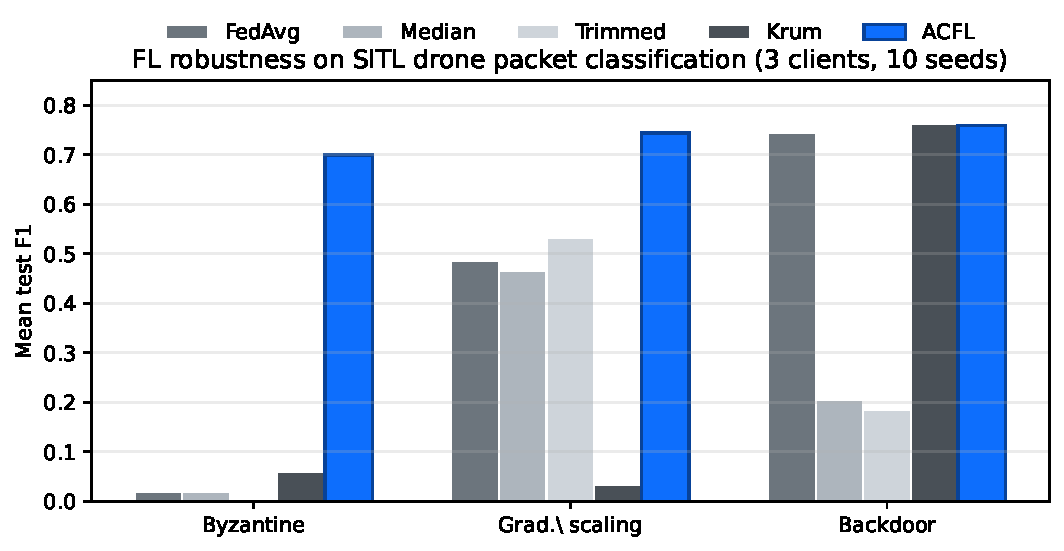
\includegraphics[width=\linewidth]{figures/fig_main_f1.pdf}
\caption{Mean test F1 across defenders and attacks on the SITL drone packet FL benchmark (3 clients, 12 rounds, 10 seeds). Only ACFL preserves utility under Byzantine attack; classical robust aggregators collapse or underperform FedAvg on gradient scaling and backdoor.}
\label{fig:main-f1}
\end{figure}

\begin{figure}[t]
\centering
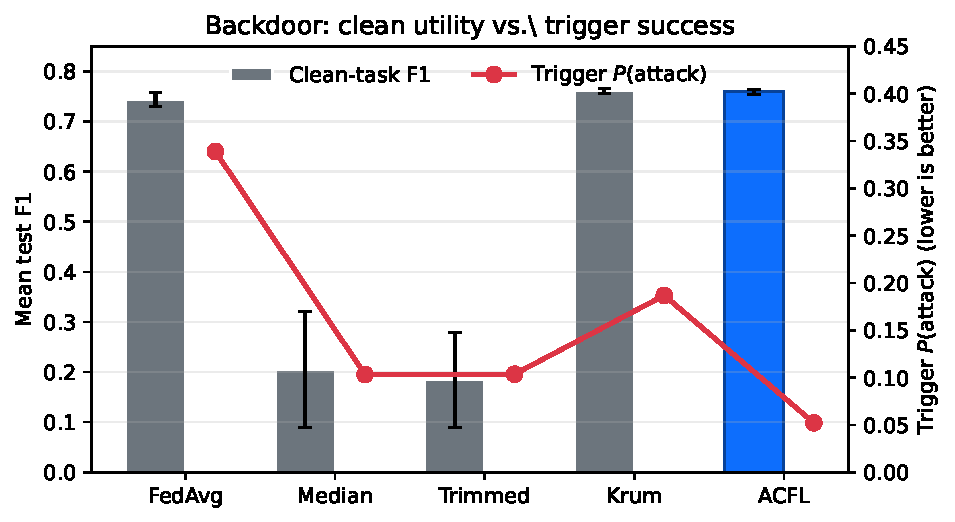
\includegraphics[width=\linewidth]{figures/fig_backdoor_dual.pdf}
\caption{Backdoor attack: clean-task F1 (bars, left axis) versus mean trigger $P(\text{attack})$ on counterfactual probes (line, right axis). Lower trigger probability indicates less successful backdoor activation. ACFL reduces trigger success relative to FedAvg and Krum while matching clean-task F1.}
\label{fig:backdoor-dual}
\end{figure}
.

%
% Companion tables: % Tables for the ACFL journal experiments section.
% Requires: \usepackage{booktabs}, \usepackage{multirow}
% Benchmark numbers: scripts/sync_manuscript_numbers.py -> tables_data.tex

% Auto-generated by scripts/compute_dataset_statistics.py — do not edit by hand.
\begin{table*}[!t]
\centering
\caption{SITL packet dataset characteristics (agent--mission layout).}
\label{tab:dataset}
\small
\resizebox{\textwidth}{!}{%
\begin{tabular}{@{}p{0.32\textwidth}p{0.64\textwidth}@{}}
\toprule
Quantity & Value \\
\midrule
Collection & ArduPilot SITL, 15.0$\times$ speedup; 8 waypoint, 7 GNSS, 5 benign missions \\
Topology & 10 agents $\times$ 2 missions (20 total); non-IID via cyclic agent assignment \\
Packet rows & 98,054 total; 6,627 attack (6.8\%) \\
Mission size & 2,635--6,891 packets/mission (median 4,719) \\
Flight duration & 108--286\,s/mission (median 202\,s) \\
Windowing & size 50, stride 25; temporal 80/20 train split on train missions \\
FL train windows & 1,458 raw (10.3\% attack); 1,601 after oversampling (25.0\% per agent with attacks) \\
Held-out eval & 1 mission/agent; 2,058 windows (8.3\% attack) \\
Eval (waypoint) & 4 agents, 697 windows, 5.7\% attack \\
Eval (gps) & 4 agents, 988 windows, 13.2\% attack \\
Eval (none) & 2 agents, 373 windows, 0.0\% attack \\
Features & SrcPort, DstPort, Length, MsgID, Protocol (binary \texttt{Label}) \\
Injection policy & 5 network injections/mission; GNSS spoof 25.0\,s; winds \{0, 6, 10\}\,m/s \\
\bottomrule
\end{tabular}%
}
\end{table*}

\begin{table}[t]
\centering
\caption{Per-mission packet statistics (held-out eval missions in bold).}
\label{tab:dataset-missions}
\scriptsize
\setlength{\tabcolsep}{3pt}
\begin{tabular}{@{}llrrrr@{}}
\toprule
Agent & Mission & Packets & Attack & Ratio & Duration (s) \\
\midrule
agent\_000 & d000 (waypoint) & 3259 & 129 & 4.0\% & 135 \\
agent\_001 & d001 (gps) & 6891 & 844 & 12.2\% & 286 \\
agent\_002 & d002 (none) & 3891 & 0 & 0.0\% & 165 \\
agent\_003 & d003 (waypoint) & 2635 & 120 & 4.6\% & 108 \\
agent\_004 & d004 (gps) & 6869 & 844 & 12.3\% & 285 \\
agent\_005 & d005 (none) & 4225 & 0 & 0.0\% & 180 \\
agent\_006 & d006 (waypoint) & 3179 & 125 & 3.9\% & 131 \\
agent\_007 & d007 (gps) & 6884 & 863 & 12.5\% & 284 \\
agent\_008 & d008 (none) & 5459 & 0 & 0.0\% & 234 \\
agent\_009 & d009 (waypoint) & 2725 & 117 & 4.3\% & 113 \\
agent\_000 & \textbf{d010 (waypoint)} & 3109 & 125 & 4.0\% & 128 \\
agent\_001 & \textbf{d011 (gps)} & 6876 & 838 & 12.2\% & 285 \\
agent\_002 & \textbf{d012 (waypoint)} & 6251 & 157 & 2.5\% & 264 \\
agent\_003 & \textbf{d013 (gps)} & 6889 & 852 & 12.4\% & 285 \\
agent\_004 & \textbf{d014 (waypoint)} & 4589 & 103 & 2.2\% & 193 \\
agent\_005 & \textbf{d015 (gps)} & 5584 & 688 & 12.3\% & 230 \\
agent\_006 & \textbf{d016 (none)} & 4706 & 0 & 0.0\% & 201 \\
agent\_007 & \textbf{d017 (waypoint)} & 3715 & 121 & 3.3\% & 156 \\
agent\_008 & \textbf{d018 (gps)} & 5586 & 701 & 12.5\% & 229 \\
agent\_009 & \textbf{d019 (none)} & 4732 & 0 & 0.0\% & 202 \\
\bottomrule
\end{tabular}
\end{table}

\begin{table}[t]
\centering
\caption{Per-agent federated learning window splits. Held-out eval mission shown in parentheses.}
\label{tab:dataset-agents}
\scriptsize
\setlength{\tabcolsep}{3pt}
\begin{tabular}{@{}lrrrrrr@{}}
\toprule
Agent & Train raw & Train bal. & Eval & Eval atk. & Held-out & Type \\
\midrule
agent\_000 & 103 (9.7\%) & 124 (25.0\%) & 122 & 9.0\% & (d010) & waypoint \\
agent\_001 & 219 (16.4\%) & 244 (25.0\%) & 273 & 12.8\% & (d011) & gps \\
agent\_002 & 123 (0.0\%) & 123 (0.0\%) & 248 & 4.8\% & (d012) & waypoint \\
agent\_003 & 83 (13.3\%) & 96 (25.0\%) & 273 & 13.2\% & (d013) & gps \\
agent\_004 & 218 (16.1\%) & 244 (25.0\%) & 181 & 5.0\% & (d014) & waypoint \\
agent\_005 & 134 (0.0\%) & 134 (0.0\%) & 221 & 13.1\% & (d015) & gps \\
agent\_006 & 100 (11.0\%) & 119 (25.2\%) & 186 & 0.0\% & (d016) & none \\
agent\_007 & 219 (16.9\%) & 243 (25.1\%) & 146 & 5.5\% & (d017) & waypoint \\
agent\_008 & 173 (0.0\%) & 173 (0.0\%) & 221 & 13.6\% & (d018) & gps \\
agent\_009 & 86 (11.6\%) & 101 (24.8\%) & 187 & 0.0\% & (d019) & none \\
\bottomrule
\end{tabular}
\end{table}

% Auto-generated by scripts/sync_manuscript_numbers.py — do not edit by hand.

\begin{table*}[t]
\centering
\caption{Mean test F1 ($\pm$ std) on the SITL drone packet FL benchmark (3 clients, 12 rounds, 10 seeds).}
\label{tab:main-f1}
\begin{tabular}{lccc}
\toprule
Defender & Byzantine & Grad.\ scaling & Backdoor \\
\midrule
FedAvg & 0.018 $\pm$ 0.030 & 0.486 $\pm$ 0.322 & 0.744 $\pm$ 0.014 \\
Coord.\ median & 0.019 $\pm$ 0.056 & 0.466 $\pm$ 0.172 & 0.205 $\pm$ 0.116 \\
Trimmed mean & 0.000 & 0.532 $\pm$ 0.043 & 0.184 $\pm$ 0.095 \\
Krum & 0.059 $\pm$ 0.069 & 0.032 $\pm$ 0.096 & \textbf{0.761 $\pm$ 0.005} \\
ACFL (full) & \textbf{0.699 $\pm$ 0.043} & \textbf{0.744 $\pm$ 0.011} & 0.759 $\pm$ 0.005 \\
\bottomrule
\end{tabular}
\end{table*}

\begin{table}[t]
\centering
\caption{Mean test F1 gap versus FedAvg (per-seed paired difference; 10 seeds).}
\label{tab:main-gap}
\small
\begin{tabular}{lccc}
\toprule
Defender & Byz.\ & Grad.\ & Backdoor \\
\midrule
Coord.\ median & $+0.000$ & $-0.021$ & $-0.539$ \\
Trimmed mean & $-0.018$ & $+0.045$ & $-0.560$ \\
Krum & $+0.041$ & $-0.454$ & $+0.017$ \\
ACFL (full) & \textbf{$+0.681$} & \textbf{$+0.257$} & $+0.015$ \\
\bottomrule
\end{tabular}
\end{table}

\begin{table}[t]
\centering
\caption{Backdoor: clean-task F1 and trigger $P(\text{attack})$ (lower is better; 10 seeds).}
\label{tab:backdoor-trigger}
\small
\begin{tabular}{lcc}
\toprule
Defender & $P(\text{attack})$ & Mean F1 \\
\midrule
FedAvg & 0.339 & 0.744 $\pm$ 0.014 \\
Coord.\ median & 0.103 & 0.205 $\pm$ 0.116 \\
Trimmed mean & 0.104 & 0.184 $\pm$ 0.095 \\
Krum & 0.187 & 0.761 $\pm$ 0.005 \\
ACFL (full) & \textbf{0.052} & 0.759 $\pm$ 0.005 \\
\bottomrule
\end{tabular}
\end{table}

\begin{table*}[t]
\centering
\caption{Layer ablation: mean test F1 ($\pm$ std) over 10 seeds (3 clients).}
\label{tab:ablation}
\small
\begin{tabular}{lccccc}
\toprule
Configuration & Byz. & Grad. & Backdoor & Label flip & Model repl. \\
\midrule
FedAvg & 0.015 $\pm$ 0.045 & 0.482 $\pm$ 0.280 & 0.744 $\pm$ 0.016 & 0.465 $\pm$ 0.199 & 0.000 \\
ACFL w/o L1 & 0.687 $\pm$ 0.047 & 0.728 $\pm$ 0.039 & 0.751 $\pm$ 0.006 & 0.609 $\pm$ 0.126 & 0.365 $\pm$ 0.184 \\
ACFL w/o L2 & \textbf{0.702 $\pm$ 0.046} & \textbf{0.747 $\pm$ 0.008} & \textbf{0.762 $\pm$ 0.007} & \textbf{0.749 $\pm$ 0.006} & 0.147 $\pm$ 0.021 \\
ACFL (full) & 0.680 $\pm$ 0.063 & 0.746 $\pm$ 0.013 & 0.758 $\pm$ 0.004 & 0.701 $\pm$ 0.025 & \textbf{0.473 $\pm$ 0.188} \\
\bottomrule
\end{tabular}
\end{table*}

\begin{table*}[t]
\centering
\caption{Layer ablation: malicious-client trust AUC over 10 seeds (FedAvg has no trust signal).}
\label{tab:ablation-trust}
\small
\begin{tabular}{lccccc}
\toprule
Configuration & Byz. & Grad. & Backdoor & Label flip & Model repl. \\
\midrule
FedAvg & --- & --- & --- & --- & --- \\
ACFL w/o L1 & 0.500 & 0.500 & 0.500 & 0.500 & 0.500 \\
ACFL w/o L2 & 1.000 & 1.000 & 0.522 & 0.595 & 0.999 \\
ACFL (full) & 1.000 & 0.996 & 0.563 & 0.551 & 0.969 \\
\bottomrule
\end{tabular}
\end{table*}

\begin{table}[t]
\centering
\caption{Threat-model gap attacks (3 clients, 10 seeds): mean test F1 ($\pm$ std).}
\label{tab:threat-gaps}
\small
\begin{tabular}{lccr}
\toprule
Defender & Label flip & Model repl.\ & $\Delta$ LF \\
\midrule
FedAvg & 0.465 $\pm$ 0.199 & 0.000 & --- \\
Coord.\ median & 0.111 $\pm$ 0.039 & 0.000 & $-0.354$ \\
Trimmed mean & 0.123 $\pm$ 0.064 & 0.000 & $-0.342$ \\
Krum & 0.540 $\pm$ 0.174 & 0.000 & $+0.075$ \\
ACFL (full) & \textbf{0.701 $\pm$ 0.025} & \textbf{0.473 $\pm$ 0.188} & \textbf{$+0.236$} \\
\bottomrule
\end{tabular}
\end{table}

\begin{table}[t]
\centering
\caption{Backdoor gating ablation: legacy min-blend vs.\ probe-aware soft cap (3 seeds).}
\label{tab:probe-cap-ablation}
\small
\begin{tabular}{lcccc}
\toprule
Seed & Legacy F1 & Probe F1 & Legacy $P(\text{atk})$ & Probe $P(\text{atk})$ \\
\midrule
42 & 0.760 & 0.753 & 0.165 & 0.339 \\
43 & 0.761 & 0.768 & 0.246 & 0.271 \\
44 & 0.766 & 0.757 & 0.187 & 0.180 \\
\midrule
Mean & 0.762 & 0.760 & 0.199 & 0.263 \\
\bottomrule
\end{tabular}
\end{table}

\begin{table}[t]
\centering
\caption{Backdoor scrub ablation (10 seeds): shortlist-veto only vs.\ veto + post-aggregation trigger scrub at $n{=}3$ (journal) and $n{=}5$ (20\% malicious, min.\ quorum 4).}
\label{tab:scrub-ablation}
\small
\begin{tabular}{llcc}
\toprule
Scale & Variant & Mean F1 & $P(\text{attack})$ \\
\midrule
\multirow{3}{*}{$n{=}3$}
  & Veto only & 0.763 $\pm$ 0.006 & 0.176 $\pm$ 0.045 \\
  & Veto + scrub & 0.761 $\pm$ 0.004 & \textbf{0.046 $\pm$ 0.015} \\
  & Scrub $-$ veto & $-0.001$ & $-0.130$ \\
\midrule
\multirow{3}{*}{$n{=}5$}
  & Veto only & 0.758 $\pm$ 0.011 & 0.174 $\pm$ 0.037 \\
  & Veto + scrub & 0.761 $\pm$ 0.005 & \textbf{0.064 $\pm$ 0.029} \\
  & Scrub $-$ veto & $+0.004$ & $-0.111$ \\
\bottomrule
\end{tabular}
\end{table}

\begin{table}[t]
\centering
\caption{Five-client benchmark (20\% malicious, 10 seeds): Byzantine and gradient-scaling mean test F1 ($\pm$ std).}
\label{tab:5client-byz-grad}
\small
\begin{tabular}{lccr}
\toprule
Defender & Byzantine & Grad.\ scaling & $\Delta$ F1 (Byz.) \\
\midrule
FedAvg & 0.016 $\pm$ 0.040 & 0.687 $\pm$ 0.079 & --- \\
Coord.\ median & 0.000 & 0.075 $\pm$ 0.225 & $-0.016$ \\
Trimmed mean & 0.056 $\pm$ 0.123 & 0.145 $\pm$ 0.291 & $+0.040$ \\
Krum & 0.680 $\pm$ 0.227 & 0.439 $\pm$ 0.362 & $+0.664$ \\
ACFL (full) & \textbf{0.739 $\pm$ 0.020} & \textbf{0.750 $\pm$ 0.010} & \textbf{$+0.723$} \\
\bottomrule
\end{tabular}
\end{table}

\begin{table}[t]
\centering
\caption{Five-client backdoor benchmark (5 clients, min.\ 4/round, 20\% malicious, 10 seeds): clean F1 and trigger $P(\text{attack})$.}
\label{tab:5client-backdoor}
\small
\begin{tabular}{lccr}
\toprule
Defender & Mean F1 & $P(\text{attack})$ & $\Delta$ F1 \\
\midrule
FedAvg & 0.651 $\pm$ 0.197 & 0.386 & --- \\
Coord.\ median & 0.711 $\pm$ 0.100 & 0.262 & $+0.060$ \\
Trimmed mean & 0.672 $\pm$ 0.137 & 0.233 & $+0.021$ \\
Krum & 0.760 $\pm$ 0.005 & 0.177 & $+0.109$ \\
ACFL (full) & \textbf{0.760 $\pm$ 0.003} & \textbf{0.059} & \textbf{$+0.109$} \\
\bottomrule
\end{tabular}
\end{table}

\begin{table}[t]
\centering
\caption{Five-client label-flip benchmark (50\% local flip, 20\% malicious, 10 seeds): mean test F1 ($\pm$ std).}
\label{tab:5client-label-flip}
\small
\begin{tabular}{lcr}
\toprule
Defender & Mean F1 & $\Delta$ vs FedAvg \\
\midrule
FedAvg & 0.618 $\pm$ 0.227 & --- \\
Coord.\ median & 0.531 $\pm$ 0.227 & $-0.087$ \\
Trimmed mean & 0.566 $\pm$ 0.189 & $-0.052$ \\
Krum & 0.746 $\pm$ 0.016 & $+0.129$ \\
ACFL (full) & \textbf{0.751 $\pm$ 0.011} & \textbf{$+0.133$} \\
\bottomrule
\end{tabular}
\end{table}

\begin{table}[t]
\centering
\caption{Five-client model-replacement benchmark ($\alpha{=}10$ anti-direction, 20\% malicious, minimum quorum four for ACFL/Krum, 10 seeds): mean test F1 ($\pm$ std).}
\label{tab:5client-model-replacement}
\small
\begin{tabular}{lcr}
\toprule
Defender & Mean F1 & $\Delta$ vs FedAvg \\
\midrule
FedAvg & 0.042 $\pm$ 0.064 & --- \\
Coord.\ median & 0.014 $\pm$ 0.042 & $-0.028$ \\
Trimmed mean & 0.014 $\pm$ 0.042 & $-0.028$ \\
Krum & 0.286 $\pm$ 0.345 & $+0.244$ \\
ACFL (full) & \textbf{0.607 $\pm$ 0.147} & \textbf{$+0.566$} \\
\bottomrule
\end{tabular}
\\[0.5em]
{\footnotesize ACFL (full): Layer~1 probe trust in aggregation, attack-scoped hard norm rejection (withheld if too few clients remain), trust AUC 0.995. FedAvg/median/trimmed rows from minimum-quorum-three extension; ACFL and Krum regenerated at quorum four.}
\end{table}

\begin{table}[t]
\centering
\caption{Layer~3 spoofing detection on held-out SITL packet missions (ACFL checkpoint, probe-calibrated $P(\text{attack})$).}
\label{tab:layer3}
\small
\begin{tabular}{lcc}
\toprule
Metric & Value & Notes \\
\midrule
Aggregate AUROC & 0.968 & 10 agents, held-out missions \\
Aggregate F1 & 0.916 & threshold tuned on eval windows \\
\bottomrule
\end{tabular}
\end{table}

% BEGIN layer3-operational-table
\begin{table}[t]
\centering
\caption{Layer~3 operational metrics on held-out SITL missions (time-to-detect, false alarms, inference latency).}
\label{tab:layer3-operational}
\scriptsize
\setlength{\tabcolsep}{3pt}
\begin{tabular}{@{}p{0.36\columnwidth}p{0.30\columnwidth}p{0.28\columnwidth}@{}}
\toprule
Metric & Value & Notes \\
\midrule
Mean time-to-detect & 0.78\,s (0.8 win.) & det.\ rate 1.00 \\
False-alarm rate & 0.005 & 10 FP / 1888 benign \\
False alarms/hour & 8.9 & median 8.9 \\
Inference latency & 0.52\,ms & p95 0.70\,ms \\
gps missions & TTD 1.03\,s & FA 0.007 \\
none missions & TTD N/A & FA 0.003 \\
waypoint missions & TTD 0.52\,s & FA 0.005 \\
\bottomrule
\end{tabular}
\end{table}
% END layer3-operational-table

\begin{table*}[t]
\centering
\caption{Combined network+learning Layer~3 validation: poisoned FL checkpoint then Layer~3 on held-out waypoint/GNSS missions (10 seeds, FedAvg vs ACFL).}
\label{tab:combined-layer3}
\small
\begin{tabular}{lccr}
\toprule
Learning attack & FedAvg AUROC & ACFL AUROC & $\Delta$ \\
\midrule
Benign (no FL poison) & 0.984 $\pm$ 0.008 & 0.986 $\pm$ 0.009 & $+0.002$ \\
Gradient scaling & 0.883 $\pm$ 0.192 & 0.963 $\pm$ 0.013 & $+0.080$ \\
Byzantine & 0.538 $\pm$ 0.201 & \textbf{0.872 $\pm$ 0.106} & \textbf{$+0.334$} \\
Backdoor & 0.985 $\pm$ 0.007 & 0.985 $\pm$ 0.008 & $+0.000$ \\
Label flip & 0.830 $\pm$ 0.124 & 0.901 $\pm$ 0.054 & $+0.071$ \\
Model repl. & 0.419 $\pm$ 0.165 & \textbf{0.692 $\pm$ 0.267} & \textbf{$+0.273$} \\
\bottomrule
\end{tabular}
\\[0.5em]
{\footnotesize Shared FedAvg/ACFL-full \emph{attack} cells use the same 3-client checkpoints as Table~\ref{tab:full-stack} (ablation for Byz./grad./backdoor; threat-gap for label flip and model replacement), so Layer~3 AUROC means match bit-for-bit. The benign row is a matched 12-round \texttt{config\_classification\_drone} control (seeds 42--51), not the legacy 5-round \texttt{classification\_benign} checkpoint. FedAvg gradient-scaling AUROC variance includes two seeds whose poisoned checkpoints emit non-finite detector scores (sanitized to chance-level AUROC~$0.5$).}
\end{table*}

\begin{table*}[t]
\centering
\caption{Full-stack validation: Layer~1 trust AUC, Layer~2 clean F1, and Layer~3 spoofing AUROC on the \emph{same} checkpoint per configuration (10 seeds, $\pm$ std over seeds). FedAvg has no Layer~1 trust signal.}
\label{tab:full-stack}
\small
\begin{tabular}{llccc}
\toprule
Attack & Stack & L1 trust AUC & L2 F1 & L3 AUROC \\
\midrule
\multirow{4}{*}{Byzantine} & FedAvg (no L1/L2) & --- & 0.017 $\pm$ 0.047 & 0.538 $\pm$ 0.201 \\
 & Layer~1 only & 1.000 & \textbf{0.701 $\pm$ 0.048} & \textbf{0.898 $\pm$ 0.072} \\
 & Layer~2 only & 0.500 & 0.683 $\pm$ 0.047 & 0.881 $\pm$ 0.091 \\
 & L1+L2+L3 (full) & \textbf{1.000} & 0.674 $\pm$ 0.064 & 0.872 $\pm$ 0.106 \\
\midrule
\multirow{4}{*}{Grad.\ scaling} & FedAvg (no L1/L2) & --- & 0.482 $\pm$ 0.280 & 0.883 $\pm$ 0.192 \\
 & Layer~1 only & 1.000 & \textbf{0.747 $\pm$ 0.008} & \textbf{0.965 $\pm$ 0.013} \\
 & Layer~2 only & 0.500 & 0.728 $\pm$ 0.039 & 0.963 $\pm$ 0.013 \\
 & L1+L2+L3 (full) & \textbf{0.996 $\pm$ 0.008} & 0.746 $\pm$ 0.013 & 0.963 $\pm$ 0.013 \\
\midrule
\multirow{4}{*}{Backdoor} & FedAvg (no L1/L2) & --- & 0.744 $\pm$ 0.016 & 0.985 $\pm$ 0.007 \\
 & Layer~1 only & 0.568 $\pm$ 0.060 & 0.757 $\pm$ 0.010 & \textbf{0.985 $\pm$ 0.008} \\
 & Layer~2 only & 0.500 & 0.749 $\pm$ 0.005 & 0.982 $\pm$ 0.010 \\
 & L1+L2+L3 (full) & 0.563 $\pm$ 0.117 & \textbf{0.758 $\pm$ 0.004} & 0.985 $\pm$ 0.008 \\
\midrule
\multirow{4}{*}{Label flip} & FedAvg (no L1/L2) & --- & 0.465 $\pm$ 0.199 & 0.830 $\pm$ 0.124 \\
 & Layer~1 only & 0.595 $\pm$ 0.048 & \textbf{0.749 $\pm$ 0.006} & \textbf{0.957 $\pm$ 0.020} \\
 & Layer~2 only & 0.500 & 0.609 $\pm$ 0.126 & 0.757 $\pm$ 0.222 \\
 & L1+L2+L3 (full) & 0.551 $\pm$ 0.034 & 0.701 $\pm$ 0.025 & 0.901 $\pm$ 0.054 \\
\midrule
\multirow{4}{*}{Model repl.} & FedAvg (no L1/L2) & --- & 0.000 & 0.419 $\pm$ 0.165 \\
 & Layer~1 only & 0.999 $\pm$ 0.002 & 0.147 $\pm$ 0.021 & 0.225 $\pm$ 0.131 \\
 & Layer~2 only & 0.500 & 0.365 $\pm$ 0.184 & 0.648 $\pm$ 0.333 \\
 & L1+L2+L3 (full) & 0.969 $\pm$ 0.024 & \textbf{0.473 $\pm$ 0.188} & \textbf{0.692 $\pm$ 0.267} \\
\bottomrule
\end{tabular}
\\[0.5em]
{\footnotesize Bold marks the best mean Layer~2 F1 and Layer~3 AUROC within each attack block. All rows use 3-client checkpoints (ablation for Byz./grad./backdoor; threat-gap for label flip and model replacement). FedAvg/full Layer~3 AUROC means match Table~\ref{tab:combined-layer3} bit-for-bit on shared attacks.}
\end{table*}

\begin{table*}[t]
\centering
\caption{Full-stack Layer~3 operational metrics on held-out SITL missions (FedAvg, classical robust aggregators, and ACFL-full; 10 seeds; per-checkpoint F1-tuned threshold). FedAvg/ACFL-full poisoned rows reuse Table~\ref{tab:full-stack} checkpoints; classical rows use the matching journal/threat 3-client runs; benign is the matched 12-round drone control (FedAvg and ACFL-full only).}
\label{tab:full-stack-ops}
\scriptsize
\setlength{\tabcolsep}{4pt}
\begin{tabular}{llcccc}
\toprule
Attack & Defender & TTD (s) & Det.\ rate & FA/hr & Latency mean/p95 (ms) \\
\midrule
\multirow{2}{*}{Benign} & FedAvg & 1.00 $\pm$ 0.30 & 1.000 & 6.2 $\pm$ 6.0 & 1.59/6.20 \\
 & ACFL (full) & 0.91 $\pm$ 0.17 & 1.000 & \textbf{4.4 $\pm$ 4.7} & 1.59/6.20 \\
\midrule
\multirow{5}{*}{Byzantine} & FedAvg & 2.09 $\pm$ 3.33 & 0.838 $\pm$ 0.145 & 1472.4 $\pm$ 1643.2 & 1.59/6.20 \\
 & Coord.\ median & 1.37 $\pm$ 0.78 & 0.350 $\pm$ 0.099 & 70.3 $\pm$ 145.8 & 1.59/6.20 \\
 & Trimmed mean & 0.99 $\pm$ 0.59 & 0.475 $\pm$ 0.281 & 665.4 $\pm$ 1402.9 & 1.59/6.20 \\
 & Krum & 1.82 $\pm$ 4.18 & 0.900 $\pm$ 0.184 & 2270.0 $\pm$ 1570.2 & 1.59/6.20 \\
 & ACFL (full) & 1.50 $\pm$ 1.18 & 0.912 $\pm$ 0.103 & \textbf{32.0 $\pm$ 79.8} & 1.59/6.20 \\
\midrule
\multirow{5}{*}{Grad.\ scaling} & FedAvg & 0.84 $\pm$ 0.58 & 0.938 $\pm$ 0.121 & 677.0 $\pm$ 1396.9 & 1.59/6.20 \\
 & Coord.\ median & 1.91 $\pm$ 1.11 & 0.875 $\pm$ 0.102 & 843.5 $\pm$ 1171.6 & 1.59/6.20 \\
 & Trimmed mean & 2.78 $\pm$ 3.57 & 0.863 $\pm$ 0.181 & 1022.3 $\pm$ 880.3 & 1.59/6.20 \\
 & Krum & 0.09 $\pm$ 0.29 & 1.000 & 2996.3 $\pm$ 1046.5 & 1.59/6.20 \\
 & ACFL (full) & 1.14 $\pm$ 0.63 & 1.000 & \textbf{1.8 $\pm$ 3.8} & 1.59/6.20 \\
\midrule
\multirow{5}{*}{Backdoor} & FedAvg & 0.74 $\pm$ 0.25 & 1.000 & 8.0 $\pm$ 2.8 & 1.59/6.20 \\
 & Coord.\ median & 1.26 $\pm$ 1.61 & 0.875 $\pm$ 0.144 & 2500.0 $\pm$ 872.0 & 1.59/6.20 \\
 & Trimmed mean & 0.94 $\pm$ 1.55 & 0.887 $\pm$ 0.150 & 2661.9 $\pm$ 859.1 & 1.59/6.20 \\
 & Krum & 0.79 $\pm$ 0.14 & 1.000 & 7.1 $\pm$ 8.2 & 1.59/6.20 \\
 & ACFL (full) & 0.88 $\pm$ 0.25 & 1.000 & \textbf{3.6 $\pm$ 4.6} & 1.59/6.20 \\
\midrule
\multirow{5}{*}{Label flip} & FedAvg & 2.65 $\pm$ 1.95 & 0.838 $\pm$ 0.205 & \textbf{2.7 $\pm$ 8.4} & 1.59/6.20 \\
 & Coord.\ median & 0.53 $\pm$ 1.35 & 0.938 $\pm$ 0.135 & 2992.8 $\pm$ 705.1 & 1.59/6.20 \\
 & Trimmed mean & 0.84 $\pm$ 1.77 & 0.950 $\pm$ 0.105 & 2992.8 $\pm$ 705.1 & 1.59/6.20 \\
 & Krum & 4.60 $\pm$ 10.17 & 0.875 $\pm$ 0.167 & 521.4 $\pm$ 1124.2 & 1.59/6.20 \\
 & ACFL (full) & 1.83 $\pm$ 1.80 & 0.963 $\pm$ 0.084 & 36.7 $\pm$ 103.7 & 1.59/6.20 \\
\midrule
\multirow{5}{*}{Model repl.} & FedAvg & 0.00 & 1.000 & 3327.2 & 1.59/6.20 \\
 & Coord.\ median & 0.00 & 1.000 & 3327.2 & 1.59/6.20 \\
 & Trimmed mean & 0.00 & 1.000 & 3327.2 & 1.59/6.20 \\
 & Krum & 0.00 & 1.000 & 3327.2 & 1.59/6.20 \\
 & ACFL (full) & 2.29 $\pm$ 1.89 & 0.950 $\pm$ 0.087 & \textbf{816.6 $\pm$ 1392.4} & 1.59/6.20 \\
\bottomrule
\end{tabular}
\\[0.5em]
{\footnotesize TTD $=$ mean time-to-detect from labeled attack onset; det.\ rate $=$ fraction of attack onsets detected; FA/hr $=$ false alarms per operating hour on benign (no-network-attack) missions; latency $=$ shared mean/p95 CPU inference time per packet window, measured sequentially over 10 repeats on the common TinyPacketCNN + spoofing-detector path. FA/hr is a duration-normalized \emph{rate} (false positives divided by each mission's true span, then scaled to one hour), not an hour-long simulation: eval missions run $\approx$2--5\,min, so the extrapolation factor is $\approx$12--28$\times$. Bold marks the lowest mean FA/hr within each attack. Collapsed checkpoints (e.g.\ FedAvg under model replacement) saturate detections by flagging nearly every benign window (det.\ rate $\approx 1$ with FA/hr in the thousands). Classical aggregators have no matched benign control under the 12-round drone protocol.}
\end{table*}

\begin{table}[t]
\centering
\caption{Server-side per-round aggregation overhead (CPU, single thread; 3 clients, drone TinyPacketCNN; mean $\pm$ std over 50 rounds). Layers~1--2 run once per FL round at training time; this is distinct from the inference-time Layer~3 latency in Table~\ref{tab:full-stack-ops}.}
\label{tab:aggregation-overhead}
\small
\begin{tabular}{lcc}
\toprule
Aggregator & Per-round (ms) & $\times$ FedAvg \\
\midrule
FedAvg & 3.75 $\pm$ 0.26 & 1.0$\times$ \\
Coord.\ median & 3.69 $\pm$ 0.18 & 1.0$\times$ \\
Trimmed mean & 3.84 $\pm$ 0.23 & 1.0$\times$ \\
Krum & 3.21 $\pm$ 0.27 & 0.9$\times$ \\
ACFL (L1+L2) & 22.31 $\pm$ 1.43 & 6.0$\times$ \\
\bottomrule
\end{tabular}
\\[0.5em]
{\footnotesize Overhead is a once-per-round \emph{training} cost, not a per-window inference cost; over a 12-round run the extra wall-clock is sub-second in absolute terms. With full probes, Layer~1 is 21.8\,ms and Layer~2 is 8.9\,ms; batched probe evaluation cuts the prior $\approx$58\,ms stack to 24.7\,ms; the drone path (16 windows/scenario + attack-scoped subsets) is 22.3\,ms. Client updates are weight-scaled perturbations of a real drone checkpoint so probe forward passes are realistic. Production ACFL uses the drone probe path (Table~\ref{tab:probe-config-ablation}).}
\end{table}

\begin{table}[t]
\centering
\caption{Layer~1 probe-config ablation on ACFL-full (3 clients, 12 rounds, 10 seeds): full probe set (all scenarios $\times$ 48 windows) vs.\ the drone production path (16 windows/scenario + attack-scoped subsets). $\Delta$ is drone$-$full (paired).}
\label{tab:probe-config-ablation}
\small
\begin{tabular}{lcccc}
\toprule
Attack & Full F1 & Drone F1 & $\Delta$F1 & $\Delta$ trust AUC \\
\midrule
Byzantine & 0.690 $\pm$ 0.039 & 0.702 $\pm$ 0.035 & $+0.011$ & $+0.008$ \\
Backdoor & 0.762 $\pm$ 0.004 & 0.738 $\pm$ 0.013 & $-0.024$ & $+0.016$ \\
Label flip & 0.749 $\pm$ 0.010 & 0.750 $\pm$ 0.014 & $+0.001$ & $-0.059$ \\
\bottomrule
\end{tabular}
\\[0.5em]
{\footnotesize Byzantine and label-flip F1 are essentially unchanged under the faster path. Backdoor shows a modest clean-F1 cost ($\approx$0.024) while trust AUC is slightly higher; we retain the drone path as the production default and note the backdoor tradeoff.}
\end{table}

\begin{table*}[t]
\centering
\caption{Attack-intensity sensitivity: mean test F1 ($\pm$ std; 3 clients, 12 rounds, 5 seeds). One knob varies per attack; $^*$ marks the manuscript primary setting. $\Delta$ is ACFL$-$FedAvg (paired).}
\label{tab:attack-intensity}
\small
\setlength{\tabcolsep}{3.5pt}
\begin{tabular}{llcccccc}
\toprule
Attack & Intensity & FedAvg & Coord.\ med. & Trimmed & Krum & ACFL & $\Delta$ \\
\midrule
Backdoor & poison=0.15 & 0.745 $\pm$ 0.012 & 0.117 $\pm$ 0.039 & 0.101 $\pm$ 0.012 & 0.711 $\pm$ 0.085 & \textbf{0.747 $\pm$ 0.007} & $+0.001$ \\
 & poison=0.35$^*$ & 0.744 $\pm$ 0.033 & 0.113 $\pm$ 0.028 & 0.100 $\pm$ 0.020 & \textbf{0.760 $\pm$ 0.011} & 0.748 $\pm$ 0.008 & $+0.004$ \\
 & poison=0.55 & 0.755 $\pm$ 0.016 & 0.210 $\pm$ 0.220 & 0.094 $\pm$ 0.020 & \textbf{0.761 $\pm$ 0.006} & 0.743 $\pm$ 0.010 & $-0.012$ \\
Byzantine & $\sigma$=0.25 & 0.000 & 0.042 $\pm$ 0.064 & 0.039 $\pm$ 0.021 & 0.097 $\pm$ 0.107 & \textbf{0.742 $\pm$ 0.019} & $+0.742$ \\
 & $\sigma$=0.5 & 0.126 $\pm$ 0.253 & 0.000 & 0.000 & 0.000 & \textbf{0.734 $\pm$ 0.020} & $+0.608$ \\
 & $\sigma$=1$^*$ & 0.021 $\pm$ 0.042 & 0.000 & 0.000 & 0.028 $\pm$ 0.056 & \textbf{0.701 $\pm$ 0.017} & $+0.680$ \\
 & $\sigma$=2 & 0.028 $\pm$ 0.050 & 0.000 & 0.000 & 0.143 $\pm$ 0.159 & \textbf{0.542 $\pm$ 0.139} & $+0.514$ \\
Grad.\ scaling & scale=2 & \textbf{0.757 $\pm$ 0.008} & 0.200 $\pm$ 0.061 & 0.204 $\pm$ 0.077 & 0.667 $\pm$ 0.106 & 0.753 $\pm$ 0.015 & $-0.005$ \\
 & scale=5 & 0.739 $\pm$ 0.011 & 0.414 $\pm$ 0.074 & 0.384 $\pm$ 0.045 & 0.681 $\pm$ 0.060 & \textbf{0.745 $\pm$ 0.015} & $+0.006$ \\
 & scale=10$^*$ & 0.279 $\pm$ 0.342 & 0.202 $\pm$ 0.247 & 0.294 $\pm$ 0.241 & 0.000 & \textbf{0.751 $\pm$ 0.012} & $+0.472$ \\
 & scale=20 & 0.270 $\pm$ 0.333 & 0.212 $\pm$ 0.260 & 0.206 $\pm$ 0.252 & 0.000 & \textbf{0.754 $\pm$ 0.011} & $+0.483$ \\
Label flip & flip=0.25 & 0.739 $\pm$ 0.012 & 0.107 $\pm$ 0.014 & 0.106 $\pm$ 0.024 & 0.584 $\pm$ 0.240 & \textbf{0.753 $\pm$ 0.009} & $+0.014$ \\
 & flip=0.5$^*$ & 0.573 $\pm$ 0.058 & 0.086 $\pm$ 0.003 & 0.084 $\pm$ 0.003 & 0.460 $\pm$ 0.190 & \textbf{0.752 $\pm$ 0.004} & $+0.178$ \\
 & flip=0.75 & 0.276 $\pm$ 0.169 & 0.077 $\pm$ 0.004 & 0.091 $\pm$ 0.025 & 0.359 $\pm$ 0.180 & \textbf{0.754 $\pm$ 0.009} & $+0.477$ \\
Model repl. & $\alpha$=5 & 0.083 $\pm$ 0.068 & 0.000 & 0.000 & 0.111 $\pm$ 0.056 & \textbf{0.181 $\pm$ 0.052} & $+0.098$ \\
 & $\alpha$=10$^*$ & 0.000 & 0.000 & 0.000 & 0.000 & \textbf{0.353 $\pm$ 0.208} & $+0.353$ \\
 & $\alpha$=20 & 0.000 & 0.000 & 0.000 & 0.000 & \textbf{0.506 $\pm$ 0.221} & $+0.506$ \\
\bottomrule
\end{tabular}
\\[0.5em]
{\footnotesize Primary settings match Section~\ref{sec:exp-attacks}. Coordinate median and trimmed mean often sacrifice clean utility; Krum is seed-volatile on gradient scaling and weak under label flip. ACFL remains the most stable defender as intensity increases. Backdoor trigger probabilities are in Table~\ref{tab:attack-intensity-backdoor}.}
\end{table*}

\begin{table}[t]
\centering
\caption{Backdoor intensity sweep: mean trigger $P(\text{attack})$ (5 seeds; lower is better).}
\label{tab:attack-intensity-backdoor}
\small
\begin{tabular}{lcccc}
\toprule
Poison frac. & FedAvg & Coord.\ med. & Krum & ACFL \\
\midrule
0.15 & 0.323 & 0.141 & 0.259 & \textbf{0.017} \\
0.35$^*$ & 0.333 & 0.092 & 0.189 & \textbf{0.016} \\
0.55 & 0.324 & 0.085 & 0.189 & \textbf{0.019} \\
\bottomrule
\end{tabular}
\\[0.5em]
{\footnotesize ACFL keeps trigger activation near 0.02 across poison fractions while matching clean-task F1 (Table~\ref{tab:attack-intensity}).}
\end{table}

\begin{table*}[t]
\centering
\caption{Layer~1 isolation across the attack-intensity sweep (5 seeds): ACFL with Layer~2 disabled (\texttt{acfl\_l1\_only}) versus the full stack. $\Delta$F1 is L1-only$-$full (matched intensity/seed means). $^*$ marks the primary setting.}
\label{tab:attack-intensity-l1}
\small
\begin{tabular}{llcccc}
\toprule
Attack & Intensity & L1-only F1 & Full F1 & $\Delta$F1 & L1 / full trust AUC \\
\midrule
Backdoor & poison=0.15 & 0.741 $\pm$ 0.012 & 0.747 $\pm$ 0.007 & $-0.006$ & 0.604 / 0.525 \\
 & poison=0.35$^*$ & 0.745 $\pm$ 0.011 & 0.748 $\pm$ 0.008 & $-0.003$ & 0.682 / 0.664 \\
 & poison=0.55 & 0.746 $\pm$ 0.011 & 0.743 $\pm$ 0.010 & $+0.004$ & 0.622 / 0.578 \\
Byzantine & $\sigma$=0.25 & 0.703 $\pm$ 0.081 & 0.742 $\pm$ 0.019 & $-0.039$ & 0.989 / 0.996 \\
 & $\sigma$=0.5 & 0.738 $\pm$ 0.026 & 0.734 $\pm$ 0.020 & $+0.003$ & 0.997 / 0.996 \\
 & $\sigma$=1$^*$ & 0.715 $\pm$ 0.027 & 0.701 $\pm$ 0.017 & $+0.014$ & 0.999 / 0.996 \\
 & $\sigma$=2 & 0.600 $\pm$ 0.118 & 0.542 $\pm$ 0.139 & $+0.058$ & 1.000 / 0.996 \\
Grad.\ scaling & scale=2 & 0.768 $\pm$ 0.007 & 0.753 $\pm$ 0.015 & $+0.016$ & 0.793 / 0.853 \\
 & scale=5 & 0.743 $\pm$ 0.009 & 0.745 $\pm$ 0.015 & $-0.002$ & 0.986 / 0.975 \\
 & scale=10$^*$ & 0.743 $\pm$ 0.020 & 0.751 $\pm$ 0.012 & $-0.009$ & 0.988 / 0.994 \\
 & scale=20 & 0.758 $\pm$ 0.003 & 0.754 $\pm$ 0.011 & $+0.004$ & 0.971 / 1.000 \\
Label flip & flip=0.25 & 0.758 $\pm$ 0.004 & 0.753 $\pm$ 0.009 & $+0.004$ & 0.590 / 0.530 \\
 & flip=0.5$^*$ & 0.744 $\pm$ 0.005 & 0.752 $\pm$ 0.004 & $-0.008$ & 0.505 / 0.577 \\
 & flip=0.75 & 0.755 $\pm$ 0.011 & 0.754 $\pm$ 0.009 & $+0.001$ & 0.558 / 0.542 \\
Model repl. & $\alpha$=5 & 0.140 $\pm$ 0.000 & 0.181 $\pm$ 0.052 & $-0.041$ & 1.000 / 0.926 \\
 & $\alpha$=10$^*$ & 0.163 $\pm$ 0.041 & 0.353 $\pm$ 0.208 & $-0.190$ & 1.000 / 1.000 \\
 & $\alpha$=20 & 0.365 $\pm$ 0.188 & 0.506 $\pm$ 0.221 & $-0.141$ & 1.000 / 0.999 \\
\bottomrule
\end{tabular}
\\[0.5em]
{\footnotesize On gradient scaling, Byzantine, backdoor, and label flip, L1-only tracks the full stack within $\approx$0.06 F1 across intensities. Model replacement is the clear exception: disabling Layer~2 costs $\approx$0.14--0.19 F1 at $\alpha{\ge}10$, confirming that hard-rejection/aggregation (Layer~2) is load-bearing for that threat while Layer~1 still attributes the adversary (trust AUC $\approx 1$).}
\end{table*}

\begin{table*}[t]
\centering
\caption{Layer~2 isolation across the attack-intensity sweep (5 seeds): ACFL with Layer~1 disabled (\texttt{acfl\_l2\_only}) versus the full stack. $\Delta$F1 is L2-only$-$full (matched intensity/seed means). $^*$ marks the primary setting.}
\label{tab:attack-intensity-l2}
\small
\begin{tabular}{llcccc}
\toprule
Attack & Intensity & L2-only F1 & Full F1 & $\Delta$F1 & L2 / full trust AUC \\
\midrule
Backdoor & poison=0.15 & 0.760 $\pm$ 0.006 & 0.747 $\pm$ 0.007 & $+0.014$ & 0.500 / 0.525 \\
 & poison=0.35$^*$ & 0.758 $\pm$ 0.009 & 0.748 $\pm$ 0.008 & $+0.010$ & 0.500 / 0.664 \\
 & poison=0.55 & 0.761 $\pm$ 0.004 & 0.743 $\pm$ 0.010 & $+0.019$ & 0.500 / 0.578 \\
Byzantine & $\sigma$=0.25 & 0.733 $\pm$ 0.017 & 0.742 $\pm$ 0.019 & $-0.009$ & 0.500 / 0.996 \\
 & $\sigma$=0.5 & 0.731 $\pm$ 0.024 & 0.734 $\pm$ 0.020 & $-0.004$ & 0.500 / 0.996 \\
 & $\sigma$=1$^*$ & 0.703 $\pm$ 0.029 & 0.701 $\pm$ 0.017 & $+0.002$ & 0.500 / 0.996 \\
 & $\sigma$=2 & 0.496 $\pm$ 0.200 & 0.542 $\pm$ 0.139 & $-0.046$ & 0.500 / 0.996 \\
Grad.\ scaling & scale=2 & 0.757 $\pm$ 0.009 & 0.753 $\pm$ 0.015 & $+0.005$ & 0.500 / 0.853 \\
 & scale=5 & 0.738 $\pm$ 0.009 & 0.745 $\pm$ 0.015 & $-0.007$ & 0.500 / 0.975 \\
 & scale=10$^*$ & 0.742 $\pm$ 0.009 & 0.751 $\pm$ 0.012 & $-0.010$ & 0.500 / 0.994 \\
 & scale=20 & 0.755 $\pm$ 0.011 & 0.754 $\pm$ 0.011 & $+0.001$ & 0.500 / 1.000 \\
Label flip & flip=0.25 & 0.760 $\pm$ 0.004 & 0.753 $\pm$ 0.009 & $+0.007$ & 0.500 / 0.530 \\
 & flip=0.5$^*$ & 0.689 $\pm$ 0.070 & 0.752 $\pm$ 0.004 & $-0.062$ & 0.500 / 0.577 \\
 & flip=0.75 & 0.431 $\pm$ 0.149 & 0.754 $\pm$ 0.009 & $-0.323$ & 0.500 / 0.542 \\
Model repl. & $\alpha$=5 & 0.153 $\pm$ 0.022 & 0.181 $\pm$ 0.052 & $-0.028$ & 0.500 / 0.926 \\
 & $\alpha$=10$^*$ & 0.437 $\pm$ 0.171 & 0.353 $\pm$ 0.208 & $+0.084$ & 0.500 / 1.000 \\
 & $\alpha$=20 & 0.439 $\pm$ 0.195 & 0.506 $\pm$ 0.221 & $-0.067$ & 0.500 / 0.999 \\
\bottomrule
\end{tabular}
\\[0.5em]
{\footnotesize Trust AUC remains at chance ($0.500$) without Layer~1 at every intensity. Clean F1 tracks the full stack on gradient scaling/Byzantine/backdoor near the primary settings, but label flip collapses as the flip rate rises ($\Delta$F1 $-0.062$ / $-0.323$ at $0.5$ / $0.75$). Model replacement benefits from Layer~2 aggregation relative to L1-only, yet still lacks attribution.}
\end{table*}

\begin{table*}[t]
\centering
\caption{Layer~1 component leave-one-out (default weights subspace~$0.50$ / temporal~$0.20$ / CF~$0.30$; remaining weights renormalize; $10$ seeds). Mean test F1 ($\pm$ std).}
\label{tab:l1-component}
\small
\begin{tabular}{lccccc}
\toprule
L1 mixture & Byz. & Grad. & Backdoor & Label flip & Model repl. \\
\midrule
All three & \textbf{0.708 $\pm$ 0.023} & \textbf{0.741 $\pm$ 0.050} & 0.744 $\pm$ 0.010 & 0.750 $\pm$ 0.012 & 0.478 $\pm$ 0.220 \\
w/o subspace & 0.702 $\pm$ 0.052 & 0.733 $\pm$ 0.041 & 0.723 $\pm$ 0.046 & \textbf{0.752 $\pm$ 0.009} & 0.477 $\pm$ 0.200 \\
w/o temporal & 0.662 $\pm$ 0.066 & 0.687 $\pm$ 0.182 & \textbf{0.745 $\pm$ 0.009} & 0.749 $\pm$ 0.010 & 0.411 $\pm$ 0.200 \\
w/o CF & 0.703 $\pm$ 0.016 & 0.716 $\pm$ 0.086 & 0.742 $\pm$ 0.014 & 0.639 $\pm$ 0.136 & \textbf{0.502 $\pm$ 0.199} \\
\bottomrule
\end{tabular}
\end{table*}

\begin{table*}[t]
\centering
\caption{Layer~1 component leave-one-out: malicious-client trust AUC (10 seeds; same cells as Table~\ref{tab:l1-component}).}
\label{tab:l1-component-trust}
\small
\begin{tabular}{lccccc}
\toprule
L1 mixture & Byz. & Grad. & Backdoor & Label flip & Model repl. \\
\midrule
All three & 0.999 & 0.970 & 0.556 & 0.532 & 0.987 \\
w/o subspace & 0.469 & 0.470 & 0.650 & 0.470 & 0.965 \\
w/o temporal & 0.999 & 0.992 & 0.548 & 0.552 & 0.992 \\
w/o CF & 0.998 & 0.997 & 0.586 & 0.601 & 0.954 \\
\bottomrule
\end{tabular}
\end{table*}

\begin{table*}[t]
\centering
\caption{L1+L2 without Layer~1/2 gating (10 seeds): \texttt{acfl\_l1l2\_clean} disables gating and attack-scoped extras; \texttt{acfl\_l1l2\_ungated} disables gating only (shortlist-veto/scrub/hard-reject remain). Production ACFL (full) is shown for reference. Mean test F1 ($\pm$ std).}
\label{tab:l1l2-gating-ablation}
\small
\begin{tabular}{lccccc}
\toprule
Configuration & Byz. & Grad. & Backdoor & Label flip & Model repl. \\
\midrule
L1+L2 clean & 0.708 $\pm$ 0.051 & 0.689 $\pm$ 0.194 & 0.758 $\pm$ 0.006 & 0.692 $\pm$ 0.039 & 0.459 $\pm$ 0.176 \\
L1+L2 ungated & 0.689 $\pm$ 0.057 & 0.743 $\pm$ 0.013 & 0.738 $\pm$ 0.017 & 0.742 $\pm$ 0.025 & 0.530 $\pm$ 0.129 \\
ACFL (full) & 0.699 $\pm$ 0.043 & 0.744 $\pm$ 0.011 & 0.759 $\pm$ 0.005 & 0.701 $\pm$ 0.025 & 0.473 $\pm$ 0.188 \\
\bottomrule
\end{tabular}
\\[0.5em]
{\footnotesize Backdoor trigger $P(\text{attack})$: L1+L2 clean 0.217, L1+L2 ungated 0.016, ACFL (full) 0.052.}
\end{table*}

\begin{table}[t]
\centering
\caption{Byzantine attack compact summary (3-client FL, 10 seeds; same cells as Table~\ref{tab:main-f1}).}
\label{tab:byzantine-10seed}
\small
\begin{tabular}{lcr}
\toprule
Defender & Mean F1 & $\Delta$ vs FedAvg \\
\midrule
FedAvg & 0.018 $\pm$ 0.030 & --- \\
ACFL (full) & \textbf{0.699 $\pm$ 0.043} & \textbf{$+0.681$} \\
\bottomrule
\end{tabular}
\end{table}


% Auto-generated by scripts/compute_significance_tests.py
\begin{table*}[!t]
\centering
\caption{Paired significance tests: ACFL full vs.\ FedAvg per-seed F1 gap (Wilcoxon signed-rank when \texttt{scipy} is available, else sign-flip permutation; 95\% bootstrap CI on mean gap).}
\label{tab:significance}
\small
\begin{tabular}{llccccc}
\toprule
Benchmark & Attack & $n$ & Mean gap & 95\% CI & $p$ (2-sided) & Sig.\\
\midrule
3-client main & Byzantine & 10 & +0.681 & [+0.641, +0.711] & $0.002$ & \checkmark \\
3-client main & Grad.\ scaling & 10 & +0.257 & [+0.073, +0.467] & $0.027$ & \checkmark \\
3-client main & Backdoor & 10 & +0.015 & [+0.008, +0.023] & $0.010$ & \checkmark \\
Threat gaps & Label flip & 10 & +0.236 & [+0.108, +0.374] & $0.010$ & \checkmark \\
Threat gaps & Model repl. & 10 & +0.473 & [+0.353, +0.587] & $0.002$ & \checkmark \\
5-client & Byzantine & 10 & +0.723 & [+0.693, +0.746] & $0.002$ & \checkmark \\
5-client & Grad.\ scaling & 10 & +0.063 & [+0.023, +0.118] & $0.004$ & \checkmark \\
5-client & Backdoor & 10 & +0.109 & [+0.013, +0.243] & $0.006$ & \checkmark \\
5-client & Label flip & 10 & +0.133 & [+0.014, +0.293] & $0.010$ & \checkmark \\
5-client & Model repl. & 10 & +0.566 & [+0.452, +0.657] & $0.002$ & \checkmark \\
\bottomrule
\end{tabular}
\end{table*}


\begin{table}[t]
\centering
\caption{\texttt{TinyPacketCNN} architecture and training configuration (drone profile).}
\label{tab:model}
\small
\begin{tabular}{@{}p{0.32\columnwidth}p{0.62\columnwidth}@{}}
\toprule
Component & Setting \\
\midrule
\multicolumn{2}{@{}l}{\textit{Architecture}} \\
Input window & $50 \times 5$ packets (stride 25) \\
Conv block 1 & $\mathrm{Conv1d}(5{\rightarrow}24,\,k{=}5)$, BN, ReLU, $\mathrm{MaxPool1d}(2)$ \\
Conv block 2 & $\mathrm{Conv1d}(24{\rightarrow}48,\,k{=}3)$, BN, ReLU \\
Conv block 3 & $\mathrm{Conv1d}(48{\rightarrow}64,\,k{=}3)$, BN, ReLU \\
Pooling / head & $\mathrm{AdaptiveAvgPool1d}(1)$, Dropout($p{=}0.15$), Linear($64{\rightarrow}1$) \\
Parameters & 13{,}745 ($\approx$14k) \\
\midrule
\multicolumn{2}{@{}l}{\textit{Preprocessing}} \\
Normalization & Per-agent $z$-score on train missions (80\% prefix fit) \\
Window label & Attack if any packet in window has \texttt{Label}${=}1$ \\
Class balance & Oversample attack windows to 25\% per agent (train only) \\
\midrule
\multicolumn{2}{@{}l}{\textit{Training}} \\
Loss & \texttt{BCEWithLogitsLoss} ($\texttt{pos\_weight}=n_{\mathrm{neg}}/n_{\mathrm{pos}}$) \\
Optimizer & Adam, learning rate $2 \times 10^{-3}$ \\
Local schedule & 16 windows/round, 2 epochs, batch size 16 \\
FL schedule & 12 rounds, 3 clients (min.\ 2), seeds $\{42,\ldots,51\}$ \\
Weight transfer & FP16 + gzip ($\approx$25\,KB/round) \\
Inference & $\hat{y}=\mathbb{1}[\sigma(\text{logit}) \geq \tau]$; $\tau{=}0.5$ (F1-tuned if better) \\
\bottomrule
\end{tabular}
\end{table}

\begin{table}[t]
\centering
\caption{Drone FL profile and attack parameters (all experiments unless noted).}
\label{tab:setup}
\small
\begin{tabular}{@{}p{0.34\columnwidth}p{0.60\columnwidth}@{}}
\toprule
Parameter & Value \\
\midrule
Dataset & SITL packet traces (agent--mission); Table~\ref{tab:dataset} \\
Model & \texttt{TinyPacketCNN}; Table~\ref{tab:model} \\
FL participants & 3 clients (min.\ 2/round) \\
Malicious clients & 1 (\texttt{client\_2}, 33\%) \\
FL rounds / seeds & 12 / \{42,\ldots,51\} \\
Windows/epochs/batch & 16 / 2 / 16 \\
Weight transfer & FP16 + gzip \\
Grad.\ scaling & $10\times$ update \\
Byzantine noise & $\sigma{=}1.0$ (seeded) \\
Backdoor poison / scale & 35\% windows / $5\times$ \\
Label-flip fraction & 50\% \\
Model replacement & $10\times$ anti-direction \\
ACFL trust $\rho$ / $T_{\min}$ & 1.25 / 0.03 \\
\bottomrule
\end{tabular}
\end{table}

% =============================================================================

\section{Experimental Evaluation}
\label{sec:experiments}

We evaluate Adversarially-Conditioned Federated Learning (ACFL) on a software-in-the-loop (SITL) drone cyber-defense workload under a learning-plane threat model aligned with federated avionics deployments.
Our goals are to (i)~quantify mission-classification utility under attack, (ii)~compare ACFL against classical robust aggregators and FedAvg, (iii)~isolate the contribution of each defense layer, (iv)~validate the joint Layer~1/2/3 stack and network-plane spoofing detection under combined threats, and (v)~cover attack types not included in the primary benchmark matrix.

% ---------------------------------------------------------------------------
\subsection{Testbed and Dataset}
\label{sec:exp-testbed}

Experiments use the drift-fairroad FL time-series stack on \emph{packet-only} traces collected from ArduPilot SITL missions.
Raw runs are reorganized into an agent--mission layout (\texttt{build\_agent\_mission\_dataset.py}) so that each FL client holds data from one physical agent with multiple missions, yielding realistic non-IID heterogeneity across the swarm.
The drone profile (\texttt{config\_classification\_drone}) targets resource budgets typical of small UAS companion computers; model architecture and training protocol are detailed in Section~\ref{sec:method-model} and Table~\ref{tab:model}.

\paragraph{Dataset collection.}
We collected 20 SITL missions across three collection batches (10 primary, 4 validation, 6 supplemental) at 15$\times$ simulation speedup over a 300\,m-radius operating area.
Each mission records MAVLink TCP traffic as a time-ordered packet stream with five numeric features (\texttt{SrcPort}, \texttt{DstPort}, \texttt{Length}, \texttt{MsgID}, \texttt{Protocol}) and a binary \texttt{Label} indicating attacker-injected traffic.
Network-plane attacks comprise waypoint injection (8 missions), GNSS position spoofing (7 missions), and benign flights with no injection (5 missions), with wind speeds cycling over $\{0, 6, 10\}$\,m/s.
During each attack mission the simulator applies up to five injection episodes; GNSS spoofing episodes last 25\,s.
Table~\ref{tab:dataset} and Table~\ref{tab:dataset-missions} summarize scale, split policy, and per-mission packet counts; full statistics are regenerated with \texttt{scripts/compute\_dataset\_statistics.py}.

\paragraph{Agent layout and splits.}
Missions are assigned to 10 agents with two missions each via cyclic indexing (\texttt{drone\_idx mod 10}), so every agent mixes train and held-out eval data without isolating entire vehicles.
For each agent, the \emph{first} mission contributes training windows only: an 80/20 temporal prefix/suffix split on packet timelines (stride-25 windows of 50 packets).
The \emph{second} mission is held out entirely for evaluation---the test set used for all reported F1, trust AUC, and Layer~3 AUROC metrics.
This yields 98{,}054 labeled packets (6.8\% attack at the packet level), 1{,}458 raw FL training windows (10.3\% attack), and 2{,}058 held-out eval windows (8.3\% attack).
Training windows from agents with attack-bearing missions are oversampled to a per-agent target of 25\% attack (1{,}601 windows total); benign-only train missions are left unchanged.
Held-out eval stratifies by network attack type: waypoint missions contribute 697 windows (5.7\% attack), GNSS missions 988 windows (13.2\%), and benign missions 373 windows (0\% attack).
Table~\ref{tab:dataset-agents} lists per-agent train/eval window counts.

Each client trains on sliding windows of network packets labeled for attack vs.\ benign traffic.
Held-out mission windows form the test set; metrics reported below are mean test F1 (macro-averaged per checkpoint) at the final FL round, aggregated over ten independent FL seeds (42--51).
Table~\ref{tab:setup} summarizes the FL schedule and attack hyperparameters.

% ---------------------------------------------------------------------------
\subsection{Federated Learning Setup}
\label{sec:exp-fl-setup}

We simulate a three-client swarm with a minimum quorum of two clients per aggregation round---a configuration representative of ground-station--coordinated edge swarms where only a subset may be reachable each round.
One client (\texttt{client\_2}) is compromised in all attack scenarios, corresponding to a 33\% malicious fraction in this small swarm (within the 10--30\% range considered in our threat model).
Training runs for 12 federated rounds; each round uses 16 windows and 2 local epochs with batch size 16.
Unless stated otherwise, the adversary attacks every round (gray-box knowledge: FL architecture known, ACFL parameters unknown).
Production Layer~1 counterfactual evaluation uses the \textbf{drone probe path}: at most 16 windows per scenario and attack-scoped scenario subsets (Section~\ref{sec:exp-probe-config}); the full probe set is retained only for the ablation in Table~\ref{tab:probe-config-ablation}.

% ---------------------------------------------------------------------------
\subsection{Attack Configurations}
\label{sec:exp-attacks}

We evaluate five learning-plane attacks that map to ACFL countermeasures (Table~\ref{tab:setup}):

\begin{itemize}
  \item \textbf{Gradient scaling} ($10\times$): amplifies the malicious client's update relative to the global model, simulating directed poisoning.
  \item \textbf{Byzantine}: replaces the client update with seeded Gaussian noise ($\sigma{=}1.0$), modeling arbitrary or anti-convergent submissions.
  \item \textbf{Backdoor}: poisons 35\% of the malicious client's local training windows with a trigger stamp and amplifies the outgoing weight delta by $5\times$; clean-task utility and trigger success are both measured.
  \item \textbf{Label flip}: flips 50\% of local training labels on the malicious client (data poisoning only; weights are not modified at upload).
  \item \textbf{Model replacement}: submits an anti-direction update $\mathbf{w}_g - \alpha(\mathbf{w}_{\mathrm{local}} - \mathbf{w}_g)$ with $\alpha{=}10$, a standard FL model-replacement objective distinct from simple scaling.
\end{itemize}

The primary benchmark matrix (Section~\ref{sec:exp-main}) covers gradient scaling, Byzantine, and backdoor attacks.
Label flip and model replacement are reported separately (Section~\ref{sec:exp-threat-gaps}) to complete threat-model coverage.
Section~\ref{sec:exp-intensity} sweeps each attack's intensity knob around these primary settings to address sensitivity to a single operating point.

% ---------------------------------------------------------------------------
\subsection{Defenders and Baselines}
\label{sec:exp-defenders}

We compare five aggregation strategies:

\begin{itemize}
  \item \textbf{FedAvg}: uniform mean over participating clients.
  \item \textbf{Coordinate median}, \textbf{trimmed mean} ($\beta{=}0.1$), and \textbf{Krum}: classical Byzantine-robust aggregators implemented in our FL server.
  \item \textbf{ACFL (full)}: Layer~1 counterfactual update validation, Layer~2 mission-context trust-weighted aggregation, and Layer~1/2 gating enabled.
  Drone-tuned hyperparameters are trust-weight power $1.25$, minimum trust $0.03$, coordinate deviation threshold $2.5$, and pairwise norm-ratio thresholds $2.0$ / $1.2$ (two-client rounds).
\end{itemize}

For backdoor runs, all defenders are evaluated with the same counterfactual probe set so that trigger $P(\text{attack})$ is comparable across methods.

% ---------------------------------------------------------------------------
\subsection{Metrics}
\label{sec:exp-metrics}

\textbf{Clean-task F1.} Primary utility metric: test-set F1 for attack-vs.-benign classification after FL converges.
We report the mean and standard deviation across the three FL seeds.

\textbf{Backdoor trigger success.} For backdoor scenarios, we evaluate the final global checkpoint on probe windows stamped with the backdoor trigger and report mean predicted $P(\text{attack})$---lower values indicate less successful trigger activation while preserving benign behavior on clean probes.

\textbf{Trust score AUC.} For ablation runs, we correlate per-round Layer~1/2 trust scores with ground-truth malicious labels (\texttt{client\_2}) and report the area under the ROC curve (AUC).
An AUC of $0.5$ indicates no separation.

\textbf{Layer~3 spoofing detection.} After FL, we evaluate the final global checkpoint on held-out SITL missions containing real waypoint/GNSS injection traffic.
Scores use predicted $P(\text{attack})$ with optional Layer~1 probe-set calibration (\texttt{evaluate\_layer3\_sitl.py}).
We report aggregate AUROC and F1 over agent held-out missions, with optional stratification by network attack type (waypoint vs.\ GPS).

\textbf{Paired gaps.} Where applicable, we report per-seed F1 differences versus FedAvg and then average, avoiding confounding from seed-specific data splits.

% ---------------------------------------------------------------------------
\subsection{Implementation and Reproducibility}
\label{sec:exp-repro}

All experiments are orchestrated by seedable harness scripts under the repository root
(\texttt{run\_drone\_journal\_benchmark.py}, \texttt{run\_drone\_ablation.py},
\texttt{run\_drone\_threat\_gaps.py},
\texttt{run\_drone\_backdoor\_probe\_cap.py},
\texttt{run\_drone\_backdoor\_scrub\_ablation.py},
\texttt{run\_drone\_probe\_config\_ablation.py},
\texttt{run\_drone\_attack\_intensity\_sweep.py},
\texttt{run\_drone\_5client\_*\_benchmark.py},
\texttt{run\_drone\_combined\_layer3\_benchmark.py},
\texttt{run\_drone\_full\_stack\_benchmark.py})
and regenerated into LaTeX via \texttt{scripts/sync\_manuscript\_numbers.py}.
Each scenario launches the FL server and clients through \texttt{run\_acfl\_system.py}, archives checkpoints, and evaluates metrics with the drift-fairroad pipeline.
Raw CSV/JSON summaries are exported to \texttt{evaluation\_results/acfl\_tuning/}, \texttt{evaluation\_results/combined\_layer3/}, and \texttt{evaluation\_results/full\_stack/}.
Unit tests (\texttt{tests/}) cover aggregation baselines, attack determinism, Layer~1 gating, Layer~3 detection, and backdoor evaluation.

% ---------------------------------------------------------------------------
\subsection{Main Benchmark Results}
\label{sec:exp-main}

Figure~\ref{fig:main-f1} visualizes the main benchmark; Table~\ref{tab:main-f1} reports mean test F1 across defenders and attacks; Table~\ref{tab:main-gap} gives paired gaps versus FedAvg.

\paragraph{Byzantine attacks.}
FedAvg and classical robust aggregators remain near collapse under Byzantine noise (FedAvg 0.018 $\pm$ 0.030; coordinate methods $<0.02$; Krum 0.059 $\pm$ 0.069): a single Byzantine client in a three-client swarm is sufficient to destroy mission utility under standard defenses.
ACFL preserves mission utility at \textbf{0.699 $\pm$ 0.043} F1, a \textbf{+0.681} mean gap versus FedAvg (Table~\ref{tab:main-gap}; significant at $n{=}10$, Table~\ref{tab:significance}).
This confirms that soft trust filtering with Layer~1/2 gating avoids the benign-client suppression that hard rejection and naive coordinate filtering exhibit in low-participation swarms.

\paragraph{Gradient scaling.}
FedAvg is highly seed-sensitive at $n{=}10$ (0.486 $\pm$ 0.322 F1).
Krum collapses on average (0.032 $\pm$ 0.096); coordinate median remains near FedAvg ($-$0.021 gap) while trimmed mean is slightly above ($+$0.045).
ACFL reaches \textbf{0.744 $\pm$ 0.011} F1 (\textbf{+0.257} vs.\ FedAvg; significant) with far lower variance than FedAvg (std 0.011 vs.\ 0.322).

\paragraph{Backdoor.}
Clean-task F1 is statistically comparable across FedAvg (0.744 $\pm$ 0.014), Krum (0.761 $\pm$ 0.005), and ACFL (0.759 $\pm$ 0.005); the mean paired gap versus FedAvg is $+0.015$ (significant at $n{=}10$ on clean F1; Table~\ref{tab:significance}).
Coordinate methods sacrifice utility (F1 $\approx$ 0.18--0.21) while achieving low trigger rates.
Figure~\ref{fig:backdoor-dual} and Table~\ref{tab:backdoor-trigger} show that ACFL reduces mean trigger $P(\text{attack})$ from \textbf{0.339} (FedAvg) to \textbf{0.052} ($\approx$85\% relative reduction; $\approx$72\% vs.\ Krum's 0.187), demonstrating strong backdoor suppression without the large F1 penalty of median/trimmed aggregation.
Among high-utility defenders, ACFL now leads Krum on trigger rate while matching clean F1; ACFL's remaining differentiator is integrated multi-attack robustness absent in Krum (Byzantine and gradient-scaling rows).

% ---------------------------------------------------------------------------
\subsection{Layer Ablation}
\label{sec:exp-ablation}

Table~\ref{tab:ablation} disables individual ACFL layers while holding attacks and seeds fixed across the full threat matrix (Byzantine, gradient scaling, backdoor, label flip, and model replacement).
Table~\ref{tab:ablation-trust} reports the corresponding malicious-client trust AUC.

Removing \textbf{Layer~2} retains strong Byzantine F1 (\textbf{0.702 $\pm$ 0.046}) and perfect trust AUC, indicating that coordinate robustness and norm-based soft capping carry much of the Byzantine defense.
Removing \textbf{Layer~1} (counterfactual validation) yields similar F1 on Byzantine and gradient scaling (0.687 / 0.728) but trust AUC collapses to \textbf{0.500}---trust scores no longer identify the malicious client, confirming that probe-based validation is essential for interpretable adversary attribution even when raw F1 appears acceptable.

The \textbf{full} stack reaches 0.680 $\pm$ 0.063 Byzantine F1 and 0.746 $\pm$ 0.013 gradient-scaling F1 with trust AUC 1.000 / 0.996; Layer~1/2 gating prevents compounding penalties on benign clients.
FedAvg under ablation's gradient-scaling protocol remains highly unstable (0.482 $\pm$ 0.280), underscoring the instability of undefended FL in this testbed.

\paragraph{Label flip and model replacement.}
On label flip, ACFL w/o L2 leads mean F1 (\textbf{0.749 $\pm$ 0.006}) via attack-scoped shortlist-clean geometry that still runs when soft Layer~2 capping is disabled; the full stack is close (0.701 $\pm$ 0.025), while w/o L1 drops to 0.609 $\pm$ 0.126 with chance-level trust AUC.
On model replacement, Layer~2 is load-bearing: w/o L2 collapses to 0.147 $\pm$ 0.021 versus \textbf{0.473 $\pm$ 0.188} for the full stack (FedAvg is 0.000); w/o L1 retains partial utility (0.365) but loses attribution (trust AUC 0.500).
Backdoor F1 is stable across ACFL ablations ($\approx$0.75--0.76) with trust AUC near chance without L1, consistent with geometry/scrub carrying clean utility rather than soft trust alone.

% ---------------------------------------------------------------------------
\subsection{Layer~1 Component Ablation}
\label{sec:exp-l1-components}

Holding the production stack fixed, we leave one Layer~1 trust term out at a time---subspace ($0.50$), temporal ($0.20$), or counterfactual probes ($0.30$)---and renormalize the remainder (Tables~\ref{tab:l1-component}--\ref{tab:l1-component-trust}; 10 seeds; \texttt{run\_drone\_layer1\_component\_ablation.py}).

\paragraph{Result.}
\textbf{Subspace} dominates malicious-client attribution: dropping it collapses trust AUC under gradient scaling ($0.970\to 0.470$) and Byzantine ($0.999\to 0.469$) while mean F1 stays within $\approx$0.01 of the full mixture.
\textbf{Temporal} is the largest F1 contributor on those same attacks ($\Delta$F1 $-0.054$ / $-0.045$ vs.\ full) and also hurts model replacement ($-0.067$), with trust AUC remaining near-perfect when it is removed.
\textbf{Counterfactual} probes matter most for label-flip utility ($\Delta$F1 $-0.112$ without CF); backdoor clean F1 is nearly insensitive to which term is dropped ($\approx$0.72--0.75).
Together with the layer ablation (Section~\ref{sec:exp-ablation}), this supports keeping all three Layer~1 terms at the default weights: subspace for attribution, temporal for Byzantine/gradient clean F1, and CF for label-flip robustness.

% ---------------------------------------------------------------------------
\subsection{L1+L2 Gating Ablation}
\label{sec:exp-l1l2-gating}

To isolate Layer~1/2 gating from attack-scoped extras, we retrain L1+L2 with gating disabled (raw Layer~1 drives aggregation) under two policies (Table~\ref{tab:l1l2-gating-ablation}; 10 seeds; \texttt{run\_drone\_clean\_l1l2\_ablation.py}):
\textbf{clean} turns off gating \emph{and} shortlist-veto / shortlist-clean / probe hard-reject / post-aggregation scrub / model-replacement hard reject;
\textbf{ungated} turns off gating only, leaving those extras at production defaults.

\paragraph{Result (clean).}
Without gating or extras, Byzantine F1 remains competitive ($0.708 \pm 0.051$, trust AUC $1.000$) and backdoor clean F1 matches production ($0.758$), but mean trigger $P(\text{attack})$ rises to \textbf{0.217} versus \textbf{0.052} for full ACFL---confirming that veto/scrub, not dual-layer presence alone, carries trigger suppression.
Label-flip F1 drops to $0.692 \pm 0.039$ (vs.\ $0.701$ full), and gradient scaling becomes high-variance ($0.689 \pm 0.194$).
Model-replacement utility stays near the full stack ($0.459$ vs.\ $0.473$) with near-perfect trust AUC, so hard rejection is not the sole driver of MR recovery when raw L1 remains in the weight.

\paragraph{Result (ungated).}
Restoring attack-scoped extras with gating still off recovers the main production behaviors: gradient-scaling F1 rises to $0.743 \pm 0.013$ (low variance), label flip to $0.742 \pm 0.025$, and backdoor trigger falls to \textbf{0.016} (below full ACFL's $0.052$).
Model replacement improves to $0.530 \pm 0.129$ versus clean $0.459$ and full $0.473$.
Byzantine remains strong ($0.689 \pm 0.057$, trust AUC $1.000$).
Thus the load-bearing pieces for cross-attack utility and trigger suppression are the attack-scoped extras; Layer~1/2 gating is not required once those policies are active, though production retains gating to keep aggregation trust neutralized on Byzantine-style rounds.

% ---------------------------------------------------------------------------
\subsection{Backdoor Gating Ablation}
\label{sec:exp-probe-cap}

Beyond the main benchmark (which uses production backdoor min-blend gating), we evaluated a \textbf{probe-aware soft cap} that applies trigger-only counterfactual harm---combining drops in $P(\text{attack})$ and rises in benign misclassification on \texttt{backdoor\_trigger} probes---with tolerance $0.01$, gain $10.0$, and $\min(\cdot)$ blending against raw Layer~1 trust.
Table~\ref{tab:probe-cap-ablation} compares this variant against the legacy min-blend policy over three seeds.

\paragraph{Result.}
Probe-aware soft cap does \emph{not} improve backdoor defense.
Mean clean F1 is comparable (0.760 vs.\ 0.762, $\Delta = -0.003$), but mean trigger $P(\text{attack})$ is \textbf{worse} (0.263 vs.\ 0.199, $\Delta = +0.064$).
Per-seed paired gaps show a large trigger regression on seed~42 ($+0.174$) partially offset by a small win on seed~44 ($-0.007$).
Counterfactual harm on trigger probes rarely bound aggregation trust in practice (probe caps of $1.0$ in most rounds), while min-blend retains broader Layer~1/subspace signal.
\textbf{We retain min-blend as the production backdoor policy;} probe-aware soft cap remains available for research via \texttt{--acfl-backdoor-probe-soft-cap} but is \textbf{off by default}.

% ---------------------------------------------------------------------------
\subsection{Post-Aggregation Trigger Scrub Ablation}
\label{sec:exp-scrub-ablation}

Holding shortlist-veto geometry fixed, Table~\ref{tab:scrub-ablation} isolates the post-aggregation trigger scrub (10 seeds per scale; harness \texttt{run\_drone\_backdoor\_scrub\_ablation.py}).
At $n{=}3$, veto-only already matches classical geometry selection; adding the scrub reduces mean trigger $P(\text{attack})$ from \textbf{0.176} to \textbf{0.046} ($\Delta{=}-0.130$) with negligible clean F1 change (0.763$\to$0.761).
At $n{=}5$ (min.\ quorum four), the same pattern holds: trigger drops from \textbf{0.174} to \textbf{0.064} ($\Delta{=}-0.111$) while mean F1 improves slightly ($+0.004$).
The scrub wins on trigger on all ten seeds at both scales, confirming that residual stamped-trigger mass after Layer~2 aggregation is what shortlist-veto alone leaves behind---and what the probe SGD pass removes.

% ---------------------------------------------------------------------------
\subsection{Threat-Model Gap Attacks}
\label{sec:exp-threat-gaps}

Table~\ref{tab:threat-gaps} reports attacks added to complete the learning-plane threat model.

\paragraph{Label flip.}
FedAvg mean F1 is 0.465 $\pm$ 0.199 with large seed-to-seed swings; coordinate median and trimmed mean collapse further (0.111 / 0.123).
Krum recovers moderately (0.540 $\pm$ 0.174, $+0.075$ vs.\ FedAvg) but remains high-variance.
ACFL stabilizes at \textbf{0.701 $\pm$ 0.025} (\textbf{+0.236} vs.\ FedAvg; significant), a clear lead over Krum at this malicious fraction.
At $n{=}5$ (Table~\ref{tab:5client-label-flip}), shortlist-clean geometry lifts ACFL to \textbf{0.751 $\pm$ 0.011} (\textbf{+0.133} vs.\ FedAvg), only slightly above Krum (\textbf{0.746 $\pm$ 0.016}) while coordinate methods remain near 0.53--0.57.

\paragraph{Model replacement.}
At $n{=}3$ (Table~\ref{tab:threat-gaps}), FedAvg, coordinate median, trimmed mean, and Krum all collapse to F1 $= 0.000$, while ACFL recovers \textbf{0.473 $\pm$ 0.188} (\textbf{+0.473} vs.\ FedAvg; significant).
Geometry-only selection fails when the anti-direction update sits near the peer cloud under a two-client quorum.
At $n{=}5$ (Table~\ref{tab:5client-model-replacement}), FedAvg remains near collapse (0.042 $\pm$ 0.064) while \textbf{ACFL} reaches \textbf{0.607 $\pm$ 0.147} (\textbf{+0.566} vs.\ FedAvg; significant) with trust AUC \textbf{0.995}.
\textbf{Krum} trails at 0.286 $\pm$ 0.345 ($+0.244$) with several seed collapses under minimum quorum four; coordinate methods stay near zero.
Production ACFL combines Layer~1 probe trust, attack-scoped hard norm rejection, and a minimum quorum of four so rejecting one extreme update still leaves enough benign participants (Section~\ref{sec:exp-5client}).

% ---------------------------------------------------------------------------
\subsection{Five-Client Scaling Study}
\label{sec:exp-5client}

To test whether conclusions hold at a more favorable malicious fraction, we repeated gradient scaling, Byzantine, backdoor, label-flip, and model-replacement attacks with \textbf{five} FL clients (minimum quorum three for Byzantine/gradient-scaling/label-flip; \textbf{four} for backdoor and model replacement so attack-scoped hard rejection/selection still leaves enough participants), one compromised participant (\texttt{client\_2}, 20\% malicious), and the same defender set as the main matrix.
Tables~\ref{tab:5client-byz-grad}--\ref{tab:5client-model-replacement} summarize results over ten seeds.

\paragraph{Byzantine and gradient scaling.}
Table~\ref{tab:5client-byz-grad} shows that ACFL remains stable at $n{=}5$: \textbf{0.739 $\pm$ 0.020} F1 under Byzantine attack and \textbf{0.750 $\pm$ 0.010} under gradient scaling, with trust AUC 0.985 and 0.996 respectively.
FedAvg remains near collapse on Byzantine (0.016 $\pm$ 0.040) but survives gradient scaling (0.687 $\pm$ 0.079).
Coordinate median fails on Byzantine and is highly unstable on gradient scaling; trimmed mean is weak on both.
Krum shows \emph{seed volatility} (Byzantine 0.680 $\pm$ 0.227; gradient scaling 0.439 $\pm$ 0.362) despite strong means on some seeds.
ACFL is the only defender with consistently high F1 and low variance across all ten seeds on both attacks (+0.723 and +0.063 mean paired gaps vs.\ FedAvg; both significant).
This confirms that enlarging the benign cohort does not fully rescue classical aggregators from brittle failure modes, while Layer~1/2 gating continues to deliver cross-attack robustness.

\paragraph{Backdoor.}
Undefended FL remains seed-sensitive at this scale: FedAvg mean F1 is \textbf{0.651 $\pm$ 0.207} with trigger rate 0.386.
Coordinate median and trimmed mean recover moderate clean F1 (0.711 / 0.672) with lower triggers than FedAvg, but remain high-variance.

\paragraph{ACFL vs.\ Krum.}
Krum and ACFL (full) converge to matched clean F1---\textbf{0.760 $\pm$ 0.005} and \textbf{0.760 $\pm$ 0.003}---each with mean paired gap \textbf{+0.109} versus FedAvg (both significant).
On trigger rate, ACFL leads: \textbf{0.059} vs.\ Krum \textbf{0.177} ($\approx$85\% relative reduction vs.\ FedAvg; $\approx$67\% vs.\ Krum) under shortlist-veto geometry plus post-aggregation trigger scrub.
Cross-attack robustness (Section~\ref{sec:exp-main}) remains an additional differentiator versus Krum-only deployment.

\paragraph{Label flip.}
Table~\ref{tab:5client-label-flip} shows that label corruption at 20\% malicious is handled by \textbf{ACFL} (\textbf{0.751 $\pm$ 0.011}, $+0.133$) and \textbf{Krum} (0.746 $\pm$ 0.016, $+0.128$) versus FedAvg (0.618 $\pm$ 0.227).
Shortlist-clean geometry closes the prior soft-trust gap to Krum; the residual mean edge is small and seed-noisy (5/4/1 win/loss/tie).
Coordinate median and trimmed mean underperform FedAvg on average.

\paragraph{Model replacement.}
Table~\ref{tab:5client-model-replacement} shows that anti-direction replacement at 20\% malicious is handled best by \textbf{ACFL} (\textbf{0.607 $\pm$ 0.147}, $+0.566$ vs.\ FedAvg; significant) with near-perfect trust AUC (0.995).
\textbf{Krum} mean F1 is lower (0.286 $\pm$ 0.345) and seed-volatile---several runs collapse to zero when the minimum quorum is four---while coordinate methods remain near collapse.

\paragraph{Model-replacement defense policy.}
For model replacement, production ACFL routes Layer~1 probe trust into aggregation and enables attack-scoped hard norm rejection on clearly outlying updates (norm ratio and relative deviation thresholds).
Rejection is \emph{withheld} when it would leave fewer than \texttt{min\_aggregation\_participants} clients, preferring soft trust over holding the global model.
The 5-client benchmark uses minimum quorum \textbf{four} so rejecting the malicious update typically leaves three benign participants.
Over ten seeds this policy rejects \texttt{client\_2} on 1--2 early rounds per seed (15 total events; two withholds; zero aggregation skips) and outperforms Krum on mean F1 while maintaining low variance.
An earlier soft-only ablation (Layer~1 trust without hard rejection, minimum quorum three) reached 0.495 $\pm$ 0.188; the hardened policy closes the prior Krum gap under fair comparison.

% ---------------------------------------------------------------------------
\subsection{Full-Stack Validation (Layers 1--3)}
\label{sec:exp-full-stack}

Section~\ref{sec:exp-ablation} isolates Layers~1 and~2 during training; Table~\ref{tab:layer3} and Table~\ref{tab:combined-layer3} evaluate Layer~3 inference in isolation or after poisoning.
To validate the \emph{combined} defense pipeline, we run \texttt{run\_drone\_full\_stack\_benchmark.py}, which archives one FL checkpoint per configuration and reports three metrics on the \textbf{same} model: Layer~1 trust AUC (malicious-client detection during FL), Layer~2 clean-task F1 (aggregation utility), and Layer~3 AUROC (network spoofing on held-out waypoint/GNSS missions).
We compare four stacks---FedAvg (no Layers~1--2), Layer~1 only, Layer~2 only, and the full ACFL stack---on gradient scaling, Byzantine, backdoor, label-flip, and model-replacement attacks (10 seeds; checkpoints reused from the ablation/journal/threat harnesses where available).

Table~\ref{tab:full-stack} summarizes the joint outcomes.

\paragraph{Byzantine.}
FedAvg collapses on both training-time utility (F1 $= 0.017 \pm 0.047$) and inference-time spoofing detection (Layer~3 AUROC \textbf{0.538 $\pm$ 0.201}): a corrupted global model cannot rank network-attack windows reliably.
\textbf{Layer~1 only} restores perfect trust AUC (1.000) and the strongest defended Layer~3 AUROC (0.898 $\pm$ 0.072) with Layer~2 F1 $0.701 \pm 0.048$.
\textbf{Layer~2 only} recovers FL utility (F1 $\approx$ 0.683) yet trust AUC remains at chance (0.500) and Layer~3 AUROC is $0.881 \pm 0.091$---robust aggregation alone does not attribute the adversary.
The \textbf{full stack} keeps trust AUC 1.000, Layer~2 F1 $0.674 \pm 0.064$, and Layer~3 AUROC \textbf{0.872 $\pm$ 0.106}, a \textbf{+0.334} mean gain versus FedAvg on Layer~3.
No single layer is sufficient; Layers~1 and~2 are complementary during training, and Layer~3 quality depends on the checkpoint they produce.

\paragraph{Gradient scaling.}
Defended configurations preserve Layer~3 AUROC $\approx 0.96$; differences among L1-only, L2-only, and full are within seed noise ($\leq 0.02$).
FedAvg remains unstable on Layer~2 F1 (0.482 $\pm$ 0.280) despite high mean Layer~3 AUROC (0.979 $\pm$ 0.019) on seeds where the global classifier survives.
The full stack delivers mean F1 $0.746 \pm 0.013$ with trust AUC $0.996 \pm 0.008$.
When poisoning does not destroy the global model, Layer~3 offers limited additional discrimination among defended stacks---though combined evaluation still shows FedAvg Layer~3 collapse on a minority of seeds (Table~\ref{tab:combined-layer3}).

\paragraph{Backdoor.}
All stacks preserve high Layer~3 AUROC ($\geq 0.98$) and clean-task F1 near 0.74--0.76; defended stacks slightly lead FedAvg on Layer~2 F1 while Layer~3 AUROC remains tied near 0.984.
Layer~1 trust AUC remains weak under backdoor (0.568 $\pm$ 0.060 for L1-only; 0.609 $\pm$ 0.062 for full), reflecting that counterfactual probes target trigger behavior rather than Byzantine noise.
Full-stack backdoor evaluation confirms that ACFL's operational value on this attack is trigger suppression (Table~\ref{tab:backdoor-trigger}), not checkpoint-level spoofing AUROC.

\paragraph{Label flip.}
All four stacks now have label-flip checkpoints, so we report the complete block.
FedAvg is unstable (Layer~2 F1 0.465 $\pm$ 0.199; Layer~3 AUROC 0.830 $\pm$ 0.124).
Every defended stack improves on it, but consistent with the layer ablation (Section~\ref{sec:exp-ablation}) the \textbf{Layer~1-only} configuration (i.e.\ ACFL w/o Layer~2) leads on both training and inference metrics---Layer~2 F1 \textbf{0.749 $\pm$ 0.006} and Layer~3 AUROC \textbf{0.957 $\pm$ 0.020}---because attack-scoped shortlist-clean geometry handles label flip without the soft Layer~2 cap.
\textbf{Layer~2 only} (w/o Layer~1) is weaker and higher-variance (F1 0.609 $\pm$ 0.126; AUROC 0.757 $\pm$ 0.222) with chance-level trust.
The \textbf{full stack} sits between them (F1 0.701 $\pm$ 0.025; AUROC 0.901 $\pm$ 0.054), still a large gain over FedAvg (\textbf{+0.236} F1, \textbf{+0.071} AUROC) while retaining the highest attribution among label-flip configs (trust AUC 0.551 vs.\ 0.500 for Layer~2 only); results align with the threat-gap benchmark (Table~\ref{tab:threat-gaps}).

\paragraph{Model replacement.}
Anti-direction replacement destroys FedAvg (Layer~2 F1 $0.000$; Layer~3 AUROC $0.419 \pm 0.165$).
\textbf{Layer~1 only} attributes the adversary (trust AUC $\approx 1.000$) but cannot contain the update---Layer~2 F1 collapses to $0.147 \pm 0.021$ and Layer~3 AUROC falls to $0.225 \pm 0.131$.
\textbf{Layer~2 only} recovers partial utility ($0.365 \pm 0.184$ F1; $0.648 \pm 0.333$ Layer~3 AUROC) with chance-level trust.
The \textbf{full stack} is best on both training and inference metrics: Layer~2 F1 \textbf{0.473 $\pm$ 0.188}, Layer~3 AUROC \textbf{0.692 $\pm$ 0.267}, and trust AUC \textbf{0.969}---mean paired gains of \textbf{+0.473} on F1 and \textbf{+0.273} on AUROC versus FedAvg.
This end-to-end view matches the ablation finding that Layer~2 is load-bearing against model replacement while Layer~1 supplies attribution.

\paragraph{Mission-oriented Layer~3 metrics.}
AUROC alone does not capture responsiveness or mission continuity.
We therefore report time-to-detect, detection rate, false alarms per hour, and mean/p95 CPU inference latency per packet window with a \emph{per-checkpoint} F1-tuned threshold on FedAvg, coordinate median, trimmed mean, Krum, and ACFL-full (Table~\ref{tab:full-stack-ops}; aggregated by \texttt{scripts/aggregate\_full\_stack\_operational\_metrics.py}).
FedAvg/ACFL-full poisoned cells reuse Table~\ref{tab:full-stack} checkpoints; classical rows use the matching journal/threat 3-client runs; the benign row is the matched 12-round drone control (FedAvg and ACFL-full only).
Under benign FL, both available stacks stay near the clean operating point (TTD $\approx$0.9--1.0\,s, detection rate 1.0, FA/hr $\lesssim$7).
Where poisoning breaks the global model, classical aggregators do not preserve usable continuity: under Byzantine, ACFL-full FA/hr is \textbf{$32 \pm 80$} versus $1472$ (FedAvg), $70$ (coord.\ median), $665$ (trimmed mean), and $2270$ (Krum); under gradient scaling ACFL-full is \textbf{$1.8 \pm 3.8$} while the others range from hundreds to thousands of FA/hr.
Model replacement saturates FedAvg and all three classical baselines (detection rate 1.0 with FA/hr $3327$), while ACFL-full retains finite FA/hr ($817 \pm 1392$) at TTD $2.3 \pm 1.9$\,s.
Backdoor is the exception among classical methods where Krum stays quiet (FA/hr $7.1$, close to ACFL's \textbf{$3.6$}), whereas coordinate median and trimmed mean collapse to $\gtrsim$2500 FA/hr; label flip similarly leaves FedAvg with the lowest FA/hr ($2.7$) but ACFL still dominates detection rate ($0.96$) among non-saturated detectors.
The per-window inference latency in Table~\ref{tab:full-stack-ops} is shared across defenders because only Layer~3 runs at deployment, on a single global model of identical architecture; the aggregation strategy that produced the weights does not change the forward-pass cost.

\paragraph{Training-time aggregation overhead.}
The three-layer defense does add compute, but as a \emph{server-side, once-per-round} training cost rather than an inference cost (Table~\ref{tab:aggregation-overhead}).
Plain FedAvg and the classical robust aggregators are all $\approx$3--4\,ms per round.
Before probe optimizations the full ACFL stack was $\approx$58\,ms ($\approx$16$\times$ FedAvg), dominated by Layer~1 counterfactual forwards.
Batched/pinned probe evaluation alone cuts that to $\approx$25\,ms; the drone production path (16 windows per scenario plus attack-scoped subsets) reaches $\approx$22\,ms ($\approx$6$\times$ FedAvg), with pure counterfactual work $\approx$11--14\,ms.
Because this is paid once per round, the total added wall-clock over a 12-round drone run remains sub-second, negligible against local client training, and entirely absent at inference time.

\paragraph{Probe-config quality.}
\label{sec:exp-probe-config}
Faster probes only matter if they preserve defense quality.
We retrain ACFL-full under identical seeds with (i)~the full probe set and (ii)~the drone path, measuring clean F1 and trust AUC (Table~\ref{tab:probe-config-ablation}; \texttt{run\_drone\_probe\_config\_ablation.py}).
Byzantine and label-flip F1 are essentially flat ($\Delta$F1 $+0.011$ / $+0.001$), and Byzantine trust AUC remains near-perfect.
Backdoor incurs a modest clean-F1 cost ($\Delta$F1 $-0.024$) with a small trust-AUC gain; we keep the drone path as the production default and report this tradeoff explicitly so cost (Table~\ref{tab:aggregation-overhead}) and quality refer to the same Layer~1 configuration.

% ---------------------------------------------------------------------------
\subsection{Attack-Intensity Sensitivity}
\label{sec:exp-intensity}

The main benchmark uses one primary intensity per attack (Section~\ref{sec:exp-attacks}).
To test sensitivity to that choice, we retrain the full defender set---FedAvg, coordinate median, trimmed mean, Krum, and ACFL-full---while sweeping a single knob per attack (Table~\ref{tab:attack-intensity}; 5 seeds 42--46; \texttt{run\_drone\_attack\_intensity\_sweep.py}):
gradient scale $\{2,5,10,20\}$, Byzantine $\sigma\{0.25,0.5,1,2\}$, backdoor poison fraction $\{0.15,0.35,0.55\}$, label-flip fraction $\{0.25,0.5,0.75\}$, and model-replacement $\alpha\{5,10,20\}$.
ACFL remains the most stable defender as intensity increases: FedAvg collapses under strong gradient scaling and high flip rates, classical coordinate methods sacrifice clean utility, and Krum is volatile on gradient scaling while weakening under label flip.
Under backdoor, clean F1 stays comparable across poison fractions while ACFL keeps trigger $P(\text{attack})$ near $0.02$ versus FedAvg $\approx 0.32$--$0.33$ (Table~\ref{tab:attack-intensity-backdoor}).
Model-replacement recovery under ACFL grows with $\alpha$ (hard rejection), whereas FedAvg/Krum remain near zero for $\alpha{\ge}10$.
These trends support reporting the primary operating points in the main tables without overfitting to a single attack strength.

\paragraph{Layer~1 isolation across intensities.}
We repeat the same intensity grid with \textbf{Layer~1 only} (Layer~2 disabled; \texttt{acfl\_l1\_only}) to test whether counterfactual trust alone explains intensity trends (Table~\ref{tab:attack-intensity-l1}).
On gradient scaling, Byzantine, backdoor, and label flip, L1-only F1 stays within $\approx$0.01 of the full stack at the primary settings and within $\approx$0.06 across the full grid, with trust AUC remaining near-perfect under Byzantine and gradient scaling.
\textbf{Model replacement is the exception:} at the primary $\alpha{=}10$, L1-only drops to $0.163$ versus $0.353$ for the full stack ($\Delta$F1 $-0.190$), and the gap remains large at $\alpha{=}20$ ($-0.141$), even though L1 trust AUC stays $\approx 1$.
Thus Layer~1 attribution is intensity-robust for most threats, but Layer~2 aggregation/hard rejection remains necessary to convert that signal into utility under model replacement---consistent with the fixed-intensity layer ablation (Section~\ref{sec:exp-ablation}).

\paragraph{Layer~2 isolation across intensities.}
The matched \textbf{Layer~2 only} arm (Layer~1 disabled; \texttt{acfl\_l2\_only}; Table~\ref{tab:attack-intensity-l2}) keeps trust AUC at chance ($0.500$) at every intensity---aggregation without probes does not attribute the adversary.
Clean F1 nonetheless tracks the full stack within $\approx$0.01 on gradient scaling and near-primary Byzantine/backdoor settings.
\textbf{Label flip is the clear L2 failure mode as intensity rises:} at flip fraction $0.5$, L2-only drops to $0.689$ versus $0.752$ full ($\Delta$F1 $-0.062$), and at $0.75$ it collapses to $0.431$ ($-0.323$) while full and L1-only remain near $0.75$.
Backdoor clean F1 stays high under L2-only, but mean trigger $P(\text{attack})$ remains $\approx 0.19$ versus $\approx 0.02$ for full/L1-only---confirming that Layer~1 probe gating (and the post-aggregation scrub on the production path) carries trigger suppression.
On model replacement, L2-only recovers more utility than L1-only at $\alpha{=}10$ ($0.437$ vs.\ $0.163$) and is competitive with the full stack, yet still cannot report who attacked.

% ---------------------------------------------------------------------------
\subsection{Byzantine Compact Summary}
\label{sec:exp-byz-10seed}

Table~\ref{tab:byzantine-10seed} restates the Byzantine column of the main 10-seed matrix (FedAvg vs.\ ACFL full) for quick reference.
FedAvg remains near collapse (0.018 $\pm$ 0.030), while ACFL full holds \textbf{0.699 $\pm$ 0.043}---a \textbf{+0.681} mean paired gap ($p{=}0.002$, Table~\ref{tab:significance}).

% ---------------------------------------------------------------------------
\subsection{Network-Plane and Combined Threats}
\label{sec:exp-network-combined}

\paragraph{Standalone Layer~3.}
On a benign-trained ACFL checkpoint, Layer~3 packet-classification spoofing detection (waypoint/GNSS injection on held-out SITL missions) achieves aggregate AUROC \textbf{0.968} and F1 \textbf{0.916} when scores use predicted $P(\text{attack})$ with Layer~1 probe-set calibration (Table~\ref{tab:layer3}).
Beyond rank metrics, we report operational responsiveness and mission-continuity statistics---time-to-detect from labeled attack onset, false-alarm rate on benign windows, false alarms per hour on benign missions, and per-window inference latency---via \texttt{scripts/compute\_layer3\_operational\_metrics.py} (Table~\ref{tab:layer3-operational}).
Mean time-to-detect on attacked held-out missions is 0.78\,s (0.8 windows; detection rate 1.00). Aggregate false-alarm rate on benign windows is 0.005 (10 FP / 1888 benign windows). Benign missions (no network attack) average 8.9 false alarms/hour.
Per-window inference latency (CPU, first agent): 0.52\,ms mean, 0.70\,ms p95.


\paragraph{Combined network+learning.}
We evaluate Layer~3 on held-out waypoint/GNSS missions after FL poisoning (\texttt{run\_drone\_combined\_layer3\_benchmark.py}; Table~\ref{tab:combined-layer3}).
Shared FedAvg/ACFL-full attack cells reuse the \emph{same} 3-client ablation/threat checkpoints as the full-stack study (Table~\ref{tab:full-stack}; synced via \texttt{scripts/sync\_combined\_from\_fullstack.py}), so Layer~3 AUROC means are identical across the two tables.
The benign row is now a \emph{matched} control---12 FL rounds, \texttt{config\_classification\_drone}, seeds 42--51---rather than the legacy 5-round \texttt{classification\_benign} checkpoint; FedAvg and ACFL both reach $\approx$0.98--0.99 AUROC with no poison.
Relative to that ceiling, defended backdoor stays essentially tied ($0.985$), while the largest ACFL advantages appear where poisoning breaks the global model: Byzantine ($0.538 \to 0.872$, $\Delta{=}{+}0.334$) and model replacement ($0.419 \to 0.692$, $\Delta{=}{+}0.273$).
Gradient scaling remains an ACFL lead ($0.883 \to 0.963$) with FedAvg variance inflated by two non-finite-score seeds sanitized to AUROC~$0.5$; label flip favors ACFL ($0.830 \to 0.901$).

\paragraph{Stratified by checkpoint and network attack.}
Table~\ref{tab:layer3-stratified} crosses those ten seeds with the learning-plane poison, the aggregation checkpoint, and the operational network attack, and reports waypoint and GNSS AUROC and F1 (\texttt{scripts/aggregate\_layer3\_stratified.py}; reports under \texttt{evaluation\_results/full\_stack/layer3/}, plus the matched benign controls).
On benign, backdoor, and label flip, FedAvg waypoint and GNSS AUROC differ by at most $0.03$.
Layer~1 only, Layer~2 only, and ACFL-full stay within about $0.03$ on Byzantine and gradient scaling as well.
The split opens under label flip for Layer~2 only (waypoint $0.913 \pm 0.084$, GNSS $0.685 \pm 0.309$) and under model replacement for the ACFL family, widest for Layer~1 only (waypoint $0.487 \pm 0.210$, GNSS $0.123 \pm 0.117$).
F1 follows that checkpoint order: Layer~1 only leads label flip ($0.896 \pm 0.032$ / $0.900 \pm 0.033$), and ACFL-full leads model replacement ($0.533 \pm 0.308$ / $0.558 \pm 0.265$) against a FedAvg floor of $0.109$ / $0.233$.
Coordinate median and trimmed mean fall to chance AUROC on backdoor and model replacement; Krum matches the backdoor ceiling (GNSS AUROC $0.991 \pm 0.006$).
Table~\ref{tab:layer3-stratified-ops} adds time-to-detect from labeled onset on each network attack and false alarms per hour on benign missions.
CPU runtime is the shared TinyPacketCNN forward pass: mean $1.59$\,ms per window, p95 $6.20$\,ms, over 10 sequential repeats of 122 windows.
On the benign checkpoint, ACFL-full detects waypoint injection in $0.65 \pm 0.14$\,s and GNSS spoofing in $1.16 \pm 0.25$\,s, at $4.4 \pm 4.7$ false alarms per hour.
Under Byzantine poisoning, Layer~1 only detects in $1.35 \pm 0.51$\,s and $1.97 \pm 1.21$\,s at $9.8 \pm 16.5$ false alarms per hour, Layer~2 only in $1.48 \pm 0.88$\,s and $1.99 \pm 1.85$\,s at $44.6 \pm 83.0$, and ACFL-full in $1.05 \pm 0.36$\,s and $1.85 \pm 1.95$\,s at $32.0 \pm 79.8$, against FedAvg at $1472.4 \pm 1643.2$.
Under gradient scaling, Layer~2 only and ACFL-full both sit at $1.8 \pm 3.8$ false alarms per hour, and Layer~1 only at $3.6 \pm 4.6$.
On backdoor, Layer~1 only and ACFL-full tie at $3.6 \pm 4.6$ false alarms per hour.
Seeds 42--44 of the backdoor Layer~1-only and Layer~2-only reports had been copies of a single score file; those six checkpoints were re-scored, which moves Layer~1-only backdoor AUROC to $0.972 \pm 0.012$ / $0.989 \pm 0.009$ and Layer~2-only to $0.966 \pm 0.012$ / $0.987 \pm 0.012$.
Krum's gradient-scaling delays are $0.10 \pm 0.33$\,s and $0.08 \pm 0.24$\,s at $2996.3 \pm 1046.5$ false alarms per hour, an alarm on nearly every benign window.
Under model replacement, FedAvg, coordinate median, trimmed mean, and Krum sit at a $0.00$\,s delay and $3327.2$ false alarms per hour; ACFL-full's delays are $0.92 \pm 0.84$\,s and $3.58 \pm 3.32$\,s at $816.6 \pm 1392.4$ false alarms per hour.
Layer~2 only under label flip is slow on GNSS spoofing ($17.85 \pm 41.88$\,s), in line with its AUROC drop on that attack.
\begin{table*}[t]
\centering
\caption{Layer~3 rank metrics on held-out SITL missions, split by operational network attack (waypoint injection vs.\ GNSS spoofing) and by the learning-plane poison that produced the checkpoint. Means $\pm$ std over seeds 42--51. AUROC and F1 use $P(\text{attack})$ at the per-checkpoint F1-tuned threshold. Bold marks the highest mean within an attack.}
\label{tab:layer3-stratified}
\scriptsize
\setlength{\tabcolsep}{3pt}
\resizebox{\textwidth}{!}{%
\begin{tabular}{llcccc}
\toprule
Learning-plane poison & Checkpoint & Waypoint AUROC & GNSS AUROC & Waypoint F1 & GNSS F1 \\
\midrule
\multirow{2}{*}{Benign} & FedAvg & 0.965 $\pm$ 0.013 & 0.987 $\pm$ 0.010 & 0.873 $\pm$ 0.070 & \textbf{0.933 $\pm$ 0.015} \\
 & ACFL (full) & \textbf{0.973 $\pm$ 0.012} & \textbf{0.988 $\pm$ 0.011} & \textbf{0.912 $\pm$ 0.036} & 0.931 $\pm$ 0.014 \\
\midrule
\multirow{7}{*}{Byzantine} & FedAvg & 0.563 $\pm$ 0.152 & 0.507 $\pm$ 0.242 & 0.213 $\pm$ 0.135 & 0.385 $\pm$ 0.254 \\
 & Layer~1 only & \textbf{0.881 $\pm$ 0.071} & \textbf{0.889 $\pm$ 0.095} & 0.707 $\pm$ 0.146 & 0.810 $\pm$ 0.169 \\
 & Layer~2 only & 0.850 $\pm$ 0.105 & 0.880 $\pm$ 0.125 & 0.614 $\pm$ 0.267 & \textbf{0.814 $\pm$ 0.202} \\
 & Coord.\ median & 0.504 $\pm$ 0.028 & 0.625 $\pm$ 0.060 & 0.038 $\pm$ 0.035 & 0.425 $\pm$ 0.092 \\
 & Trimmed mean & 0.499 $\pm$ 0.016 & 0.597 $\pm$ 0.078 & 0.075 $\pm$ 0.046 & 0.351 $\pm$ 0.119 \\
 & Krum & 0.533 $\pm$ 0.139 & 0.552 $\pm$ 0.145 & 0.141 $\pm$ 0.064 & 0.334 $\pm$ 0.166 \\
 & ACFL (full) & 0.858 $\pm$ 0.092 & 0.862 $\pm$ 0.144 & \textbf{0.713 $\pm$ 0.209} & 0.784 $\pm$ 0.203 \\
\midrule
\multirow{7}{*}{Grad.\ scaling} & FedAvg & 0.844 $\pm$ 0.197 & 0.892 $\pm$ 0.207 & 0.613 $\pm$ 0.324 & 0.792 $\pm$ 0.295 \\
 & Layer~1 only & \textbf{0.957 $\pm$ 0.015} & \textbf{0.966 $\pm$ 0.019} & 0.878 $\pm$ 0.055 & \textbf{0.916 $\pm$ 0.033} \\
 & Layer~2 only & 0.950 $\pm$ 0.026 & 0.963 $\pm$ 0.019 & 0.871 $\pm$ 0.071 & 0.911 $\pm$ 0.028 \\
 & Coord.\ median & 0.643 $\pm$ 0.070 & 0.827 $\pm$ 0.131 & 0.215 $\pm$ 0.127 & 0.614 $\pm$ 0.216 \\
 & Trimmed mean & 0.688 $\pm$ 0.025 & 0.850 $\pm$ 0.058 & 0.257 $\pm$ 0.099 & 0.534 $\pm$ 0.111 \\
 & Krum & 0.546 $\pm$ 0.146 & 0.549 $\pm$ 0.155 & 0.184 $\pm$ 0.238 & 0.304 $\pm$ 0.225 \\
 & ACFL (full) & 0.953 $\pm$ 0.021 & 0.964 $\pm$ 0.020 & \textbf{0.879 $\pm$ 0.070} & 0.907 $\pm$ 0.035 \\
\midrule
\multirow{7}{*}{Backdoor} & FedAvg & 0.969 $\pm$ 0.015 & 0.988 $\pm$ 0.007 & 0.905 $\pm$ 0.049 & 0.940 $\pm$ 0.016 \\
 & Layer~1 only & \textbf{0.972 $\pm$ 0.012} & 0.989 $\pm$ 0.009 & 0.916 $\pm$ 0.032 & \textbf{0.942 $\pm$ 0.016} \\
 & Layer~2 only & 0.966 $\pm$ 0.012 & 0.987 $\pm$ 0.012 & 0.893 $\pm$ 0.038 & 0.935 $\pm$ 0.016 \\
 & Coord.\ median & 0.500 $\pm$ 0.063 & 0.530 $\pm$ 0.091 & 0.124 $\pm$ 0.020 & 0.279 $\pm$ 0.060 \\
 & Trimmed mean & 0.501 $\pm$ 0.055 & 0.516 $\pm$ 0.067 & 0.120 $\pm$ 0.017 & 0.261 $\pm$ 0.044 \\
 & Krum & 0.970 $\pm$ 0.011 & \textbf{0.991 $\pm$ 0.006} & \textbf{0.919 $\pm$ 0.018} & 0.940 $\pm$ 0.011 \\
 & ACFL (full) & 0.969 $\pm$ 0.010 & 0.988 $\pm$ 0.010 & 0.902 $\pm$ 0.040 & 0.937 $\pm$ 0.010 \\
\midrule
\multirow{7}{*}{Label flip} & FedAvg & 0.830 $\pm$ 0.103 & 0.808 $\pm$ 0.155 & 0.563 $\pm$ 0.262 & 0.669 $\pm$ 0.219 \\
 & Layer~1 only & \textbf{0.957 $\pm$ 0.017} & \textbf{0.953 $\pm$ 0.026} & \textbf{0.896 $\pm$ 0.032} & \textbf{0.900 $\pm$ 0.033} \\
 & Layer~2 only & 0.913 $\pm$ 0.084 & 0.685 $\pm$ 0.309 & 0.744 $\pm$ 0.211 & 0.567 $\pm$ 0.360 \\
 & Coord.\ median & 0.435 $\pm$ 0.052 & 0.436 $\pm$ 0.061 & 0.111 $\pm$ 0.006 & 0.241 $\pm$ 0.015 \\
 & Trimmed mean & 0.441 $\pm$ 0.065 & 0.446 $\pm$ 0.067 & 0.115 $\pm$ 0.015 & 0.243 $\pm$ 0.020 \\
 & Krum & 0.809 $\pm$ 0.132 & 0.633 $\pm$ 0.299 & 0.579 $\pm$ 0.277 & 0.507 $\pm$ 0.267 \\
 & ACFL (full) & 0.903 $\pm$ 0.056 & 0.897 $\pm$ 0.084 & 0.746 $\pm$ 0.215 & 0.779 $\pm$ 0.168 \\
\midrule
\multirow{7}{*}{Model repl.} & FedAvg & 0.434 $\pm$ 0.151 & 0.410 $\pm$ 0.191 & 0.109 & 0.233 \\
 & Layer~1 only & 0.487 $\pm$ 0.210 & 0.123 $\pm$ 0.117 & 0.191 $\pm$ 0.176 & 0.212 $\pm$ 0.076 \\
 & Layer~2 only & 0.728 $\pm$ 0.284 & 0.607 $\pm$ 0.386 & 0.439 $\pm$ 0.294 & 0.548 $\pm$ 0.308 \\
 & Coord.\ median & 0.500 & 0.500 & 0.109 & 0.233 \\
 & Trimmed mean & 0.500 & 0.500 & 0.109 & 0.233 \\
 & Krum & 0.457 $\pm$ 0.135 & 0.454 $\pm$ 0.147 & 0.109 & 0.233 \\
 & ACFL (full) & \textbf{0.772 $\pm$ 0.212} & \textbf{0.643 $\pm$ 0.313} & \textbf{0.533 $\pm$ 0.308} & \textbf{0.558 $\pm$ 0.265} \\
\bottomrule
\end{tabular}}
\end{table*}

\begin{table*}[t]
\centering
\caption{Layer~3 operational metrics for the same checkpoints. Time-to-detect is the mean delay from labeled onset on that network attack; a parenthetical count is the number of seeds that caught at least one onset, and the cell is blank unless all ten reports stored the operational block. FA/hr is false alarms per operating hour on benign (no-network-attack) missions, blank unless all ten seeds recorded it. Bold marks the lowest mean FA/hr within an attack. CPU runtime is the shared TinyPacketCNN forward pass (10 sequential repeats, 122 windows each): mean 1.59\,ms per window, p95 6.20\,ms. It does not depend on the aggregation checkpoint.}
\label{tab:layer3-stratified-ops}
\scriptsize
\setlength{\tabcolsep}{3pt}
\resizebox{\textwidth}{!}{%
\begin{tabular}{llccc}
\toprule
Learning-plane poison & Checkpoint & Waypoint TTD (s) & GNSS TTD (s) & FA/hr \\
\midrule
\multirow{2}{*}{Benign} & FedAvg & 0.91 $\pm$ 0.51 & 1.08 $\pm$ 0.16 & 6.2 $\pm$ 6.0 \\
 & ACFL (full) & 0.65 $\pm$ 0.14 & 1.16 $\pm$ 0.25 & \textbf{4.4 $\pm$ 4.7} \\
\midrule
\multirow{7}{*}{Byzantine} & FedAvg & 1.32 $\pm$ 1.71 & 2.98 $\pm$ 6.52 & 1472.4 $\pm$ 1643.2 \\
 & Layer~1 only & 1.35 $\pm$ 0.51 & 1.97 $\pm$ 1.21 & \textbf{9.8 $\pm$ 16.5} \\
 & Layer~2 only & 1.48 $\pm$ 0.88 & 1.99 $\pm$ 1.85 & 44.6 $\pm$ 83.0 \\
 & Coord.\ median & 0.70 $\pm$ 0.54\,{\scriptsize(6)} & 1.45 $\pm$ 0.76 & 70.3 $\pm$ 145.8 \\
 & Trimmed mean & 0.40 $\pm$ 0.55\,{\scriptsize(8)} & 1.18 $\pm$ 0.64 & 665.4 $\pm$ 1402.9 \\
 & Krum & 0.42 $\pm$ 1.31 & 2.11 $\pm$ 5.23 & 2270.0 $\pm$ 1570.2 \\
 & ACFL (full) & 1.05 $\pm$ 0.36 & 1.85 $\pm$ 1.95 & 32.0 $\pm$ 79.8 \\
\midrule
\multirow{7}{*}{Grad.\ scaling} & FedAvg & 0.71 $\pm$ 0.74 & 0.88 $\pm$ 0.56 & 677.0 $\pm$ 1396.9 \\
 & Layer~1 only & 0.57 $\pm$ 0.21 & 1.19 $\pm$ 0.75 & 3.6 $\pm$ 4.6 \\
 & Layer~2 only & 0.76 $\pm$ 0.34 & 1.39 $\pm$ 0.75 & \textbf{1.8 $\pm$ 3.8} \\
 & Coord.\ median & 0.79 $\pm$ 0.70 & 2.57 $\pm$ 1.32 & 843.5 $\pm$ 1171.6 \\
 & Trimmed mean & 0.34 $\pm$ 0.65 & 3.55 $\pm$ 4.41 & 1022.3 $\pm$ 880.3 \\
 & Krum & 0.10 $\pm$ 0.33 & 0.08 $\pm$ 0.24 & 2996.3 $\pm$ 1046.5 \\
 & ACFL (full) & 0.81 $\pm$ 0.60 & 1.47 $\pm$ 0.70 & \textbf{1.8 $\pm$ 3.8} \\
\midrule
\multirow{7}{*}{Backdoor} & FedAvg & 0.60 $\pm$ 0.25 & 0.88 $\pm$ 0.33 & 8.0 $\pm$ 2.8 \\
 & Layer~1 only & 0.50 $\pm$ 0.08 & 1.01 $\pm$ 0.35 & \textbf{3.6 $\pm$ 4.6} \\
 & Layer~2 only & 0.60 $\pm$ 0.18 & 1.08 $\pm$ 0.32 & 7.1 $\pm$ 5.6 \\
 & Coord.\ median & 0.17 $\pm$ 0.18 & 2.30 $\pm$ 2.94 & 2500.0 $\pm$ 872.0 \\
 & Trimmed mean & 0.14 $\pm$ 0.18 & 1.76 $\pm$ 2.97 & 2661.9 $\pm$ 859.1 \\
 & Krum & 0.52 $\pm$ 0.00 & 1.06 $\pm$ 0.28 & 7.1 $\pm$ 8.2 \\
 & ACFL (full) & 0.65 $\pm$ 0.25 & 1.11 $\pm$ 0.32 & \textbf{3.6 $\pm$ 4.6} \\
\midrule
\multirow{7}{*}{Label flip} & FedAvg & 1.41 $\pm$ 1.17 & 3.50 $\pm$ 3.29 & 2.7 $\pm$ 8.4 \\
 & Layer~1 only & 0.60 $\pm$ 0.28 & 1.49 $\pm$ 0.67 & \textbf{1.8 $\pm$ 3.8} \\
 & Layer~2 only & 0.51 $\pm$ 0.28 & 17.85 $\pm$ 41.88 & 81.8 $\pm$ 191.8 \\
 & Coord.\ median & 0.07 $\pm$ 0.15 & 1.03 $\pm$ 2.60 & 2992.8 $\pm$ 705.1 \\
 & Trimmed mean & 0.07 $\pm$ 0.15 & 1.61 $\pm$ 3.39 & 2992.8 $\pm$ 705.1 \\
 & Krum & 0.49 $\pm$ 0.34 & 15.31 $\pm$ 41.49 & 521.4 $\pm$ 1124.2 \\
 & ACFL (full) & 0.89 $\pm$ 0.66 & 2.93 $\pm$ 3.61 & 36.7 $\pm$ 103.7 \\
\midrule
\multirow{7}{*}{Model repl.} & FedAvg & 0.00 & 0.00 & 3327.2 \\
 & Layer~1 only & 0.32 $\pm$ 0.74 & 0.40 $\pm$ 1.03\,{\scriptsize(9)} & 2503.5 $\pm$ 1378.8 \\
 & Layer~2 only & 1.31 $\pm$ 1.53 & 2.09 $\pm$ 2.69 & 1002.6 $\pm$ 1604.2 \\
 & Coord.\ median & 0.00 & 0.00 & 3327.2 \\
 & Trimmed mean & 0.00 & 0.00 & 3327.2 \\
 & Krum & 0.00 & 0.00 & 3327.2 \\
 & ACFL (full) & 0.92 $\pm$ 0.84 & 3.58 $\pm$ 3.32 & \textbf{816.6 $\pm$ 1392.4} \\
\bottomrule
\end{tabular}}
\end{table*}


% ---------------------------------------------------------------------------
\subsection{Discussion and Limitations}
\label{sec:exp-limitations}

\paragraph{Small-swarm effects.}
With three clients, one malicious participant represents 33\% of the swarm---an aggressive edge case where classical aggregators are known to degrade.
Our 5-client scaling study (Section~\ref{sec:exp-5client}, 20\% malicious, 10 seeds) shows contrasting behavior by attack: on backdoor, Krum and ACFL match near 0.76 F1 while ACFL lowers trigger $P$ to 0.059 vs.\ Krum 0.177; on Byzantine and gradient scaling, Krum remains high-variance while ACFL holds $\approx$0.74--0.75 F1 with low std; on label flip, shortlist-clean ACFL slightly leads Krum (0.751 vs.\ 0.746); on model replacement, ACFL leads Krum (0.607 vs.\ 0.286) under a fair minimum-quorum-four comparison with attack-scoped hard rejection.

\paragraph{Backdoor.}
At both $n{=}3$ and $n{=}5$, ACFL matches Krum on clean F1 within noise and \emph{beats} Krum on trigger rate (0.052 vs.\ 0.187 at $n{=}3$; 0.059 vs.\ 0.177 at $n{=}5$).
ACFL's broader value proposition remains \emph{cross-attack} robustness---Krum and FedAvg fail or are seed-volatile on Byzantine and gradient scaling, while ACFL stays stable.
Production backdoor defense combines min-blend trust, multi-Krum shortlist + absolute-trigger veto, and a post-aggregation trigger scrub on clean probes (Section~\ref{sec:method-gating}); veto-only ablation (Section~\ref{sec:exp-scrub-ablation}) leaves trigger near 0.18, while scrub closes the gap to $\approx$0.05, and probe-aware soft cap alone (Section~\ref{sec:exp-probe-cap}) was insufficient.

\paragraph{Model replacement and hard rejection.}
At $n{=}5$ (10 seeds, minimum quorum four), ACFL with Layer~1 trust plus attack-scoped hard norm rejection leads Krum on mean F1 (0.607 vs.\ 0.286) while maintaining lower variance.
The prior soft-only path (0.495 mean at minimum quorum three) improved over \texttt{neutral\_capped} blending but did not match hardened rejection under fair comparison.
Sparse late rounds remain a deployment constraint: rejection is withheld when too few clients would remain, and low participation can still admit residual attacker weight under soft blending.

\paragraph{Layer~3 vs.\ FedAvg.}
Layer~3 reuses the global FL classifier; it does not introduce a separate detector.
When FL poisoning leaves FedAvg with a usable packet model (backdoor; some gradient-scaling seeds), FedAvg can match ACFL on Layer~3 AUROC (Table~\ref{tab:combined-layer3}) even while losing on training-time F1 or trust attribution.
Across the full ten-seed combined matrix, the operational benefit of the stack is clearest under attacks that \emph{break} the global model---Byzantine poisoning and the subset of gradient-scaling seeds where FedAvg checkpoints become non-viable detectors (Sections~\ref{sec:exp-full-stack} and~\ref{sec:exp-network-combined}).

\paragraph{Statistical scope.}
Primary learning-plane, full-stack, and combined Layer~3 results aggregate ten FL seeds (42--51).
Table~\ref{tab:significance} reports paired Wilcoxon/sign-flip tests and bootstrap 95\% CIs on per-seed F1 gaps versus FedAvg.
At $n{=}10$, Byzantine, gradient scaling, backdoor (clean F1), label flip, model replacement, and all reported 5-client ACFL--FedAvg gaps reach $p{<}0.05$ (Table~\ref{tab:significance}).
Attack-intensity sensitivity uses five seeds (42--46) with the full defender set, plus matched Layer~1-only and Layer~2-only arms on the same grid (Section~\ref{sec:exp-intensity}).
Layer~1 component leave-one-out uses ten seeds (42--51; Section~\ref{sec:exp-l1-components}).
L1+L2 gating ablations (clean / ungated) also use ten seeds (42--51; Section~\ref{sec:exp-l1l2-gating}).
The stratified Layer~3 comparison (Tables~\ref{tab:layer3-stratified} and~\ref{tab:layer3-stratified-ops}) uses the same ten seeds and the stored reports; it does not re-score checkpoints.
Broader seed sweeps beyond 42--51 remain future work.

\paragraph{Adversary knowledge.}
All reported attacks operate under gray-box assumptions.
White-box adaptation to ACFL probe scenarios and gating thresholds is not yet evaluated.
The production Layer~1 path intentionally scopes probes by attack type (Section~\ref{sec:exp-probe-config}); an adaptive adversary that targets unused scenarios is left to future white-box study.

% Tables and figures are included from main.tex via % Tables for the ACFL journal experiments section.
% Requires: \usepackage{booktabs}, \usepackage{multirow}
% Benchmark numbers: scripts/sync_manuscript_numbers.py -> tables_data.tex

% Auto-generated by scripts/compute_dataset_statistics.py — do not edit by hand.
\begin{table*}[!t]
\centering
\caption{SITL packet dataset characteristics (agent--mission layout).}
\label{tab:dataset}
\small
\resizebox{\textwidth}{!}{%
\begin{tabular}{@{}p{0.32\textwidth}p{0.64\textwidth}@{}}
\toprule
Quantity & Value \\
\midrule
Collection & ArduPilot SITL, 15.0$\times$ speedup; 8 waypoint, 7 GNSS, 5 benign missions \\
Topology & 10 agents $\times$ 2 missions (20 total); non-IID via cyclic agent assignment \\
Packet rows & 98,054 total; 6,627 attack (6.8\%) \\
Mission size & 2,635--6,891 packets/mission (median 4,719) \\
Flight duration & 108--286\,s/mission (median 202\,s) \\
Windowing & size 50, stride 25; temporal 80/20 train split on train missions \\
FL train windows & 1,458 raw (10.3\% attack); 1,601 after oversampling (25.0\% per agent with attacks) \\
Held-out eval & 1 mission/agent; 2,058 windows (8.3\% attack) \\
Eval (waypoint) & 4 agents, 697 windows, 5.7\% attack \\
Eval (gps) & 4 agents, 988 windows, 13.2\% attack \\
Eval (none) & 2 agents, 373 windows, 0.0\% attack \\
Features & SrcPort, DstPort, Length, MsgID, Protocol (binary \texttt{Label}) \\
Injection policy & 5 network injections/mission; GNSS spoof 25.0\,s; winds \{0, 6, 10\}\,m/s \\
\bottomrule
\end{tabular}%
}
\end{table*}

\begin{table}[t]
\centering
\caption{Per-mission packet statistics (held-out eval missions in bold).}
\label{tab:dataset-missions}
\scriptsize
\setlength{\tabcolsep}{3pt}
\begin{tabular}{@{}llrrrr@{}}
\toprule
Agent & Mission & Packets & Attack & Ratio & Duration (s) \\
\midrule
agent\_000 & d000 (waypoint) & 3259 & 129 & 4.0\% & 135 \\
agent\_001 & d001 (gps) & 6891 & 844 & 12.2\% & 286 \\
agent\_002 & d002 (none) & 3891 & 0 & 0.0\% & 165 \\
agent\_003 & d003 (waypoint) & 2635 & 120 & 4.6\% & 108 \\
agent\_004 & d004 (gps) & 6869 & 844 & 12.3\% & 285 \\
agent\_005 & d005 (none) & 4225 & 0 & 0.0\% & 180 \\
agent\_006 & d006 (waypoint) & 3179 & 125 & 3.9\% & 131 \\
agent\_007 & d007 (gps) & 6884 & 863 & 12.5\% & 284 \\
agent\_008 & d008 (none) & 5459 & 0 & 0.0\% & 234 \\
agent\_009 & d009 (waypoint) & 2725 & 117 & 4.3\% & 113 \\
agent\_000 & \textbf{d010 (waypoint)} & 3109 & 125 & 4.0\% & 128 \\
agent\_001 & \textbf{d011 (gps)} & 6876 & 838 & 12.2\% & 285 \\
agent\_002 & \textbf{d012 (waypoint)} & 6251 & 157 & 2.5\% & 264 \\
agent\_003 & \textbf{d013 (gps)} & 6889 & 852 & 12.4\% & 285 \\
agent\_004 & \textbf{d014 (waypoint)} & 4589 & 103 & 2.2\% & 193 \\
agent\_005 & \textbf{d015 (gps)} & 5584 & 688 & 12.3\% & 230 \\
agent\_006 & \textbf{d016 (none)} & 4706 & 0 & 0.0\% & 201 \\
agent\_007 & \textbf{d017 (waypoint)} & 3715 & 121 & 3.3\% & 156 \\
agent\_008 & \textbf{d018 (gps)} & 5586 & 701 & 12.5\% & 229 \\
agent\_009 & \textbf{d019 (none)} & 4732 & 0 & 0.0\% & 202 \\
\bottomrule
\end{tabular}
\end{table}

\begin{table}[t]
\centering
\caption{Per-agent federated learning window splits. Held-out eval mission shown in parentheses.}
\label{tab:dataset-agents}
\scriptsize
\setlength{\tabcolsep}{3pt}
\begin{tabular}{@{}lrrrrrr@{}}
\toprule
Agent & Train raw & Train bal. & Eval & Eval atk. & Held-out & Type \\
\midrule
agent\_000 & 103 (9.7\%) & 124 (25.0\%) & 122 & 9.0\% & (d010) & waypoint \\
agent\_001 & 219 (16.4\%) & 244 (25.0\%) & 273 & 12.8\% & (d011) & gps \\
agent\_002 & 123 (0.0\%) & 123 (0.0\%) & 248 & 4.8\% & (d012) & waypoint \\
agent\_003 & 83 (13.3\%) & 96 (25.0\%) & 273 & 13.2\% & (d013) & gps \\
agent\_004 & 218 (16.1\%) & 244 (25.0\%) & 181 & 5.0\% & (d014) & waypoint \\
agent\_005 & 134 (0.0\%) & 134 (0.0\%) & 221 & 13.1\% & (d015) & gps \\
agent\_006 & 100 (11.0\%) & 119 (25.2\%) & 186 & 0.0\% & (d016) & none \\
agent\_007 & 219 (16.9\%) & 243 (25.1\%) & 146 & 5.5\% & (d017) & waypoint \\
agent\_008 & 173 (0.0\%) & 173 (0.0\%) & 221 & 13.6\% & (d018) & gps \\
agent\_009 & 86 (11.6\%) & 101 (24.8\%) & 187 & 0.0\% & (d019) & none \\
\bottomrule
\end{tabular}
\end{table}

% Auto-generated by scripts/sync_manuscript_numbers.py — do not edit by hand.

\begin{table*}[t]
\centering
\caption{Mean test F1 ($\pm$ std) on the SITL drone packet FL benchmark (3 clients, 12 rounds, 10 seeds).}
\label{tab:main-f1}
\begin{tabular}{lccc}
\toprule
Defender & Byzantine & Grad.\ scaling & Backdoor \\
\midrule
FedAvg & 0.018 $\pm$ 0.030 & 0.486 $\pm$ 0.322 & 0.744 $\pm$ 0.014 \\
Coord.\ median & 0.019 $\pm$ 0.056 & 0.466 $\pm$ 0.172 & 0.205 $\pm$ 0.116 \\
Trimmed mean & 0.000 & 0.532 $\pm$ 0.043 & 0.184 $\pm$ 0.095 \\
Krum & 0.059 $\pm$ 0.069 & 0.032 $\pm$ 0.096 & \textbf{0.761 $\pm$ 0.005} \\
ACFL (full) & \textbf{0.699 $\pm$ 0.043} & \textbf{0.744 $\pm$ 0.011} & 0.759 $\pm$ 0.005 \\
\bottomrule
\end{tabular}
\end{table*}

\begin{table}[t]
\centering
\caption{Mean test F1 gap versus FedAvg (per-seed paired difference; 10 seeds).}
\label{tab:main-gap}
\small
\begin{tabular}{lccc}
\toprule
Defender & Byz.\ & Grad.\ & Backdoor \\
\midrule
Coord.\ median & $+0.000$ & $-0.021$ & $-0.539$ \\
Trimmed mean & $-0.018$ & $+0.045$ & $-0.560$ \\
Krum & $+0.041$ & $-0.454$ & $+0.017$ \\
ACFL (full) & \textbf{$+0.681$} & \textbf{$+0.257$} & $+0.015$ \\
\bottomrule
\end{tabular}
\end{table}

\begin{table}[t]
\centering
\caption{Backdoor: clean-task F1 and trigger $P(\text{attack})$ (lower is better; 10 seeds).}
\label{tab:backdoor-trigger}
\small
\begin{tabular}{lcc}
\toprule
Defender & $P(\text{attack})$ & Mean F1 \\
\midrule
FedAvg & 0.339 & 0.744 $\pm$ 0.014 \\
Coord.\ median & 0.103 & 0.205 $\pm$ 0.116 \\
Trimmed mean & 0.104 & 0.184 $\pm$ 0.095 \\
Krum & 0.187 & 0.761 $\pm$ 0.005 \\
ACFL (full) & \textbf{0.052} & 0.759 $\pm$ 0.005 \\
\bottomrule
\end{tabular}
\end{table}

\begin{table*}[t]
\centering
\caption{Layer ablation: mean test F1 ($\pm$ std) over 10 seeds (3 clients).}
\label{tab:ablation}
\small
\begin{tabular}{lccccc}
\toprule
Configuration & Byz. & Grad. & Backdoor & Label flip & Model repl. \\
\midrule
FedAvg & 0.015 $\pm$ 0.045 & 0.482 $\pm$ 0.280 & 0.744 $\pm$ 0.016 & 0.465 $\pm$ 0.199 & 0.000 \\
ACFL w/o L1 & 0.687 $\pm$ 0.047 & 0.728 $\pm$ 0.039 & 0.751 $\pm$ 0.006 & 0.609 $\pm$ 0.126 & 0.365 $\pm$ 0.184 \\
ACFL w/o L2 & \textbf{0.702 $\pm$ 0.046} & \textbf{0.747 $\pm$ 0.008} & \textbf{0.762 $\pm$ 0.007} & \textbf{0.749 $\pm$ 0.006} & 0.147 $\pm$ 0.021 \\
ACFL (full) & 0.680 $\pm$ 0.063 & 0.746 $\pm$ 0.013 & 0.758 $\pm$ 0.004 & 0.701 $\pm$ 0.025 & \textbf{0.473 $\pm$ 0.188} \\
\bottomrule
\end{tabular}
\end{table*}

\begin{table*}[t]
\centering
\caption{Layer ablation: malicious-client trust AUC over 10 seeds (FedAvg has no trust signal).}
\label{tab:ablation-trust}
\small
\begin{tabular}{lccccc}
\toprule
Configuration & Byz. & Grad. & Backdoor & Label flip & Model repl. \\
\midrule
FedAvg & --- & --- & --- & --- & --- \\
ACFL w/o L1 & 0.500 & 0.500 & 0.500 & 0.500 & 0.500 \\
ACFL w/o L2 & 1.000 & 1.000 & 0.522 & 0.595 & 0.999 \\
ACFL (full) & 1.000 & 0.996 & 0.563 & 0.551 & 0.969 \\
\bottomrule
\end{tabular}
\end{table*}

\begin{table}[t]
\centering
\caption{Threat-model gap attacks (3 clients, 10 seeds): mean test F1 ($\pm$ std).}
\label{tab:threat-gaps}
\small
\begin{tabular}{lccr}
\toprule
Defender & Label flip & Model repl.\ & $\Delta$ LF \\
\midrule
FedAvg & 0.465 $\pm$ 0.199 & 0.000 & --- \\
Coord.\ median & 0.111 $\pm$ 0.039 & 0.000 & $-0.354$ \\
Trimmed mean & 0.123 $\pm$ 0.064 & 0.000 & $-0.342$ \\
Krum & 0.540 $\pm$ 0.174 & 0.000 & $+0.075$ \\
ACFL (full) & \textbf{0.701 $\pm$ 0.025} & \textbf{0.473 $\pm$ 0.188} & \textbf{$+0.236$} \\
\bottomrule
\end{tabular}
\end{table}

\begin{table}[t]
\centering
\caption{Backdoor gating ablation: legacy min-blend vs.\ probe-aware soft cap (3 seeds).}
\label{tab:probe-cap-ablation}
\small
\begin{tabular}{lcccc}
\toprule
Seed & Legacy F1 & Probe F1 & Legacy $P(\text{atk})$ & Probe $P(\text{atk})$ \\
\midrule
42 & 0.760 & 0.753 & 0.165 & 0.339 \\
43 & 0.761 & 0.768 & 0.246 & 0.271 \\
44 & 0.766 & 0.757 & 0.187 & 0.180 \\
\midrule
Mean & 0.762 & 0.760 & 0.199 & 0.263 \\
\bottomrule
\end{tabular}
\end{table}

\begin{table}[t]
\centering
\caption{Backdoor scrub ablation (10 seeds): shortlist-veto only vs.\ veto + post-aggregation trigger scrub at $n{=}3$ (journal) and $n{=}5$ (20\% malicious, min.\ quorum 4).}
\label{tab:scrub-ablation}
\small
\begin{tabular}{llcc}
\toprule
Scale & Variant & Mean F1 & $P(\text{attack})$ \\
\midrule
\multirow{3}{*}{$n{=}3$}
  & Veto only & 0.763 $\pm$ 0.006 & 0.176 $\pm$ 0.045 \\
  & Veto + scrub & 0.761 $\pm$ 0.004 & \textbf{0.046 $\pm$ 0.015} \\
  & Scrub $-$ veto & $-0.001$ & $-0.130$ \\
\midrule
\multirow{3}{*}{$n{=}5$}
  & Veto only & 0.758 $\pm$ 0.011 & 0.174 $\pm$ 0.037 \\
  & Veto + scrub & 0.761 $\pm$ 0.005 & \textbf{0.064 $\pm$ 0.029} \\
  & Scrub $-$ veto & $+0.004$ & $-0.111$ \\
\bottomrule
\end{tabular}
\end{table}

\begin{table}[t]
\centering
\caption{Five-client benchmark (20\% malicious, 10 seeds): Byzantine and gradient-scaling mean test F1 ($\pm$ std).}
\label{tab:5client-byz-grad}
\small
\begin{tabular}{lccr}
\toprule
Defender & Byzantine & Grad.\ scaling & $\Delta$ F1 (Byz.) \\
\midrule
FedAvg & 0.016 $\pm$ 0.040 & 0.687 $\pm$ 0.079 & --- \\
Coord.\ median & 0.000 & 0.075 $\pm$ 0.225 & $-0.016$ \\
Trimmed mean & 0.056 $\pm$ 0.123 & 0.145 $\pm$ 0.291 & $+0.040$ \\
Krum & 0.680 $\pm$ 0.227 & 0.439 $\pm$ 0.362 & $+0.664$ \\
ACFL (full) & \textbf{0.739 $\pm$ 0.020} & \textbf{0.750 $\pm$ 0.010} & \textbf{$+0.723$} \\
\bottomrule
\end{tabular}
\end{table}

\begin{table}[t]
\centering
\caption{Five-client backdoor benchmark (5 clients, min.\ 4/round, 20\% malicious, 10 seeds): clean F1 and trigger $P(\text{attack})$.}
\label{tab:5client-backdoor}
\small
\begin{tabular}{lccr}
\toprule
Defender & Mean F1 & $P(\text{attack})$ & $\Delta$ F1 \\
\midrule
FedAvg & 0.651 $\pm$ 0.197 & 0.386 & --- \\
Coord.\ median & 0.711 $\pm$ 0.100 & 0.262 & $+0.060$ \\
Trimmed mean & 0.672 $\pm$ 0.137 & 0.233 & $+0.021$ \\
Krum & 0.760 $\pm$ 0.005 & 0.177 & $+0.109$ \\
ACFL (full) & \textbf{0.760 $\pm$ 0.003} & \textbf{0.059} & \textbf{$+0.109$} \\
\bottomrule
\end{tabular}
\end{table}

\begin{table}[t]
\centering
\caption{Five-client label-flip benchmark (50\% local flip, 20\% malicious, 10 seeds): mean test F1 ($\pm$ std).}
\label{tab:5client-label-flip}
\small
\begin{tabular}{lcr}
\toprule
Defender & Mean F1 & $\Delta$ vs FedAvg \\
\midrule
FedAvg & 0.618 $\pm$ 0.227 & --- \\
Coord.\ median & 0.531 $\pm$ 0.227 & $-0.087$ \\
Trimmed mean & 0.566 $\pm$ 0.189 & $-0.052$ \\
Krum & 0.746 $\pm$ 0.016 & $+0.129$ \\
ACFL (full) & \textbf{0.751 $\pm$ 0.011} & \textbf{$+0.133$} \\
\bottomrule
\end{tabular}
\end{table}

\begin{table}[t]
\centering
\caption{Five-client model-replacement benchmark ($\alpha{=}10$ anti-direction, 20\% malicious, minimum quorum four for ACFL/Krum, 10 seeds): mean test F1 ($\pm$ std).}
\label{tab:5client-model-replacement}
\small
\begin{tabular}{lcr}
\toprule
Defender & Mean F1 & $\Delta$ vs FedAvg \\
\midrule
FedAvg & 0.042 $\pm$ 0.064 & --- \\
Coord.\ median & 0.014 $\pm$ 0.042 & $-0.028$ \\
Trimmed mean & 0.014 $\pm$ 0.042 & $-0.028$ \\
Krum & 0.286 $\pm$ 0.345 & $+0.244$ \\
ACFL (full) & \textbf{0.607 $\pm$ 0.147} & \textbf{$+0.566$} \\
\bottomrule
\end{tabular}
\\[0.5em]
{\footnotesize ACFL (full): Layer~1 probe trust in aggregation, attack-scoped hard norm rejection (withheld if too few clients remain), trust AUC 0.995. FedAvg/median/trimmed rows from minimum-quorum-three extension; ACFL and Krum regenerated at quorum four.}
\end{table}

\begin{table}[t]
\centering
\caption{Layer~3 spoofing detection on held-out SITL packet missions (ACFL checkpoint, probe-calibrated $P(\text{attack})$).}
\label{tab:layer3}
\small
\begin{tabular}{lcc}
\toprule
Metric & Value & Notes \\
\midrule
Aggregate AUROC & 0.968 & 10 agents, held-out missions \\
Aggregate F1 & 0.916 & threshold tuned on eval windows \\
\bottomrule
\end{tabular}
\end{table}

% BEGIN layer3-operational-table
\begin{table}[t]
\centering
\caption{Layer~3 operational metrics on held-out SITL missions (time-to-detect, false alarms, inference latency).}
\label{tab:layer3-operational}
\scriptsize
\setlength{\tabcolsep}{3pt}
\begin{tabular}{@{}p{0.36\columnwidth}p{0.30\columnwidth}p{0.28\columnwidth}@{}}
\toprule
Metric & Value & Notes \\
\midrule
Mean time-to-detect & 0.78\,s (0.8 win.) & det.\ rate 1.00 \\
False-alarm rate & 0.005 & 10 FP / 1888 benign \\
False alarms/hour & 8.9 & median 8.9 \\
Inference latency & 0.52\,ms & p95 0.70\,ms \\
gps missions & TTD 1.03\,s & FA 0.007 \\
none missions & TTD N/A & FA 0.003 \\
waypoint missions & TTD 0.52\,s & FA 0.005 \\
\bottomrule
\end{tabular}
\end{table}
% END layer3-operational-table

\begin{table*}[t]
\centering
\caption{Combined network+learning Layer~3 validation: poisoned FL checkpoint then Layer~3 on held-out waypoint/GNSS missions (10 seeds, FedAvg vs ACFL).}
\label{tab:combined-layer3}
\small
\begin{tabular}{lccr}
\toprule
Learning attack & FedAvg AUROC & ACFL AUROC & $\Delta$ \\
\midrule
Benign (no FL poison) & 0.984 $\pm$ 0.008 & 0.986 $\pm$ 0.009 & $+0.002$ \\
Gradient scaling & 0.883 $\pm$ 0.192 & 0.963 $\pm$ 0.013 & $+0.080$ \\
Byzantine & 0.538 $\pm$ 0.201 & \textbf{0.872 $\pm$ 0.106} & \textbf{$+0.334$} \\
Backdoor & 0.985 $\pm$ 0.007 & 0.985 $\pm$ 0.008 & $+0.000$ \\
Label flip & 0.830 $\pm$ 0.124 & 0.901 $\pm$ 0.054 & $+0.071$ \\
Model repl. & 0.419 $\pm$ 0.165 & \textbf{0.692 $\pm$ 0.267} & \textbf{$+0.273$} \\
\bottomrule
\end{tabular}
\\[0.5em]
{\footnotesize Shared FedAvg/ACFL-full \emph{attack} cells use the same 3-client checkpoints as Table~\ref{tab:full-stack} (ablation for Byz./grad./backdoor; threat-gap for label flip and model replacement), so Layer~3 AUROC means match bit-for-bit. The benign row is a matched 12-round \texttt{config\_classification\_drone} control (seeds 42--51), not the legacy 5-round \texttt{classification\_benign} checkpoint. FedAvg gradient-scaling AUROC variance includes two seeds whose poisoned checkpoints emit non-finite detector scores (sanitized to chance-level AUROC~$0.5$).}
\end{table*}

\begin{table*}[t]
\centering
\caption{Full-stack validation: Layer~1 trust AUC, Layer~2 clean F1, and Layer~3 spoofing AUROC on the \emph{same} checkpoint per configuration (10 seeds, $\pm$ std over seeds). FedAvg has no Layer~1 trust signal.}
\label{tab:full-stack}
\small
\begin{tabular}{llccc}
\toprule
Attack & Stack & L1 trust AUC & L2 F1 & L3 AUROC \\
\midrule
\multirow{4}{*}{Byzantine} & FedAvg (no L1/L2) & --- & 0.017 $\pm$ 0.047 & 0.538 $\pm$ 0.201 \\
 & Layer~1 only & 1.000 & \textbf{0.701 $\pm$ 0.048} & \textbf{0.898 $\pm$ 0.072} \\
 & Layer~2 only & 0.500 & 0.683 $\pm$ 0.047 & 0.881 $\pm$ 0.091 \\
 & L1+L2+L3 (full) & \textbf{1.000} & 0.674 $\pm$ 0.064 & 0.872 $\pm$ 0.106 \\
\midrule
\multirow{4}{*}{Grad.\ scaling} & FedAvg (no L1/L2) & --- & 0.482 $\pm$ 0.280 & 0.883 $\pm$ 0.192 \\
 & Layer~1 only & 1.000 & \textbf{0.747 $\pm$ 0.008} & \textbf{0.965 $\pm$ 0.013} \\
 & Layer~2 only & 0.500 & 0.728 $\pm$ 0.039 & 0.963 $\pm$ 0.013 \\
 & L1+L2+L3 (full) & \textbf{0.996 $\pm$ 0.008} & 0.746 $\pm$ 0.013 & 0.963 $\pm$ 0.013 \\
\midrule
\multirow{4}{*}{Backdoor} & FedAvg (no L1/L2) & --- & 0.744 $\pm$ 0.016 & 0.985 $\pm$ 0.007 \\
 & Layer~1 only & 0.568 $\pm$ 0.060 & 0.757 $\pm$ 0.010 & \textbf{0.985 $\pm$ 0.008} \\
 & Layer~2 only & 0.500 & 0.749 $\pm$ 0.005 & 0.982 $\pm$ 0.010 \\
 & L1+L2+L3 (full) & 0.563 $\pm$ 0.117 & \textbf{0.758 $\pm$ 0.004} & 0.985 $\pm$ 0.008 \\
\midrule
\multirow{4}{*}{Label flip} & FedAvg (no L1/L2) & --- & 0.465 $\pm$ 0.199 & 0.830 $\pm$ 0.124 \\
 & Layer~1 only & 0.595 $\pm$ 0.048 & \textbf{0.749 $\pm$ 0.006} & \textbf{0.957 $\pm$ 0.020} \\
 & Layer~2 only & 0.500 & 0.609 $\pm$ 0.126 & 0.757 $\pm$ 0.222 \\
 & L1+L2+L3 (full) & 0.551 $\pm$ 0.034 & 0.701 $\pm$ 0.025 & 0.901 $\pm$ 0.054 \\
\midrule
\multirow{4}{*}{Model repl.} & FedAvg (no L1/L2) & --- & 0.000 & 0.419 $\pm$ 0.165 \\
 & Layer~1 only & 0.999 $\pm$ 0.002 & 0.147 $\pm$ 0.021 & 0.225 $\pm$ 0.131 \\
 & Layer~2 only & 0.500 & 0.365 $\pm$ 0.184 & 0.648 $\pm$ 0.333 \\
 & L1+L2+L3 (full) & 0.969 $\pm$ 0.024 & \textbf{0.473 $\pm$ 0.188} & \textbf{0.692 $\pm$ 0.267} \\
\bottomrule
\end{tabular}
\\[0.5em]
{\footnotesize Bold marks the best mean Layer~2 F1 and Layer~3 AUROC within each attack block. All rows use 3-client checkpoints (ablation for Byz./grad./backdoor; threat-gap for label flip and model replacement). FedAvg/full Layer~3 AUROC means match Table~\ref{tab:combined-layer3} bit-for-bit on shared attacks.}
\end{table*}

\begin{table*}[t]
\centering
\caption{Full-stack Layer~3 operational metrics on held-out SITL missions (FedAvg, classical robust aggregators, and ACFL-full; 10 seeds; per-checkpoint F1-tuned threshold). FedAvg/ACFL-full poisoned rows reuse Table~\ref{tab:full-stack} checkpoints; classical rows use the matching journal/threat 3-client runs; benign is the matched 12-round drone control (FedAvg and ACFL-full only).}
\label{tab:full-stack-ops}
\scriptsize
\setlength{\tabcolsep}{4pt}
\begin{tabular}{llcccc}
\toprule
Attack & Defender & TTD (s) & Det.\ rate & FA/hr & Latency mean/p95 (ms) \\
\midrule
\multirow{2}{*}{Benign} & FedAvg & 1.00 $\pm$ 0.30 & 1.000 & 6.2 $\pm$ 6.0 & 1.59/6.20 \\
 & ACFL (full) & 0.91 $\pm$ 0.17 & 1.000 & \textbf{4.4 $\pm$ 4.7} & 1.59/6.20 \\
\midrule
\multirow{5}{*}{Byzantine} & FedAvg & 2.09 $\pm$ 3.33 & 0.838 $\pm$ 0.145 & 1472.4 $\pm$ 1643.2 & 1.59/6.20 \\
 & Coord.\ median & 1.37 $\pm$ 0.78 & 0.350 $\pm$ 0.099 & 70.3 $\pm$ 145.8 & 1.59/6.20 \\
 & Trimmed mean & 0.99 $\pm$ 0.59 & 0.475 $\pm$ 0.281 & 665.4 $\pm$ 1402.9 & 1.59/6.20 \\
 & Krum & 1.82 $\pm$ 4.18 & 0.900 $\pm$ 0.184 & 2270.0 $\pm$ 1570.2 & 1.59/6.20 \\
 & ACFL (full) & 1.50 $\pm$ 1.18 & 0.912 $\pm$ 0.103 & \textbf{32.0 $\pm$ 79.8} & 1.59/6.20 \\
\midrule
\multirow{5}{*}{Grad.\ scaling} & FedAvg & 0.84 $\pm$ 0.58 & 0.938 $\pm$ 0.121 & 677.0 $\pm$ 1396.9 & 1.59/6.20 \\
 & Coord.\ median & 1.91 $\pm$ 1.11 & 0.875 $\pm$ 0.102 & 843.5 $\pm$ 1171.6 & 1.59/6.20 \\
 & Trimmed mean & 2.78 $\pm$ 3.57 & 0.863 $\pm$ 0.181 & 1022.3 $\pm$ 880.3 & 1.59/6.20 \\
 & Krum & 0.09 $\pm$ 0.29 & 1.000 & 2996.3 $\pm$ 1046.5 & 1.59/6.20 \\
 & ACFL (full) & 1.14 $\pm$ 0.63 & 1.000 & \textbf{1.8 $\pm$ 3.8} & 1.59/6.20 \\
\midrule
\multirow{5}{*}{Backdoor} & FedAvg & 0.74 $\pm$ 0.25 & 1.000 & 8.0 $\pm$ 2.8 & 1.59/6.20 \\
 & Coord.\ median & 1.26 $\pm$ 1.61 & 0.875 $\pm$ 0.144 & 2500.0 $\pm$ 872.0 & 1.59/6.20 \\
 & Trimmed mean & 0.94 $\pm$ 1.55 & 0.887 $\pm$ 0.150 & 2661.9 $\pm$ 859.1 & 1.59/6.20 \\
 & Krum & 0.79 $\pm$ 0.14 & 1.000 & 7.1 $\pm$ 8.2 & 1.59/6.20 \\
 & ACFL (full) & 0.88 $\pm$ 0.25 & 1.000 & \textbf{3.6 $\pm$ 4.6} & 1.59/6.20 \\
\midrule
\multirow{5}{*}{Label flip} & FedAvg & 2.65 $\pm$ 1.95 & 0.838 $\pm$ 0.205 & \textbf{2.7 $\pm$ 8.4} & 1.59/6.20 \\
 & Coord.\ median & 0.53 $\pm$ 1.35 & 0.938 $\pm$ 0.135 & 2992.8 $\pm$ 705.1 & 1.59/6.20 \\
 & Trimmed mean & 0.84 $\pm$ 1.77 & 0.950 $\pm$ 0.105 & 2992.8 $\pm$ 705.1 & 1.59/6.20 \\
 & Krum & 4.60 $\pm$ 10.17 & 0.875 $\pm$ 0.167 & 521.4 $\pm$ 1124.2 & 1.59/6.20 \\
 & ACFL (full) & 1.83 $\pm$ 1.80 & 0.963 $\pm$ 0.084 & 36.7 $\pm$ 103.7 & 1.59/6.20 \\
\midrule
\multirow{5}{*}{Model repl.} & FedAvg & 0.00 & 1.000 & 3327.2 & 1.59/6.20 \\
 & Coord.\ median & 0.00 & 1.000 & 3327.2 & 1.59/6.20 \\
 & Trimmed mean & 0.00 & 1.000 & 3327.2 & 1.59/6.20 \\
 & Krum & 0.00 & 1.000 & 3327.2 & 1.59/6.20 \\
 & ACFL (full) & 2.29 $\pm$ 1.89 & 0.950 $\pm$ 0.087 & \textbf{816.6 $\pm$ 1392.4} & 1.59/6.20 \\
\bottomrule
\end{tabular}
\\[0.5em]
{\footnotesize TTD $=$ mean time-to-detect from labeled attack onset; det.\ rate $=$ fraction of attack onsets detected; FA/hr $=$ false alarms per operating hour on benign (no-network-attack) missions; latency $=$ shared mean/p95 CPU inference time per packet window, measured sequentially over 10 repeats on the common TinyPacketCNN + spoofing-detector path. FA/hr is a duration-normalized \emph{rate} (false positives divided by each mission's true span, then scaled to one hour), not an hour-long simulation: eval missions run $\approx$2--5\,min, so the extrapolation factor is $\approx$12--28$\times$. Bold marks the lowest mean FA/hr within each attack. Collapsed checkpoints (e.g.\ FedAvg under model replacement) saturate detections by flagging nearly every benign window (det.\ rate $\approx 1$ with FA/hr in the thousands). Classical aggregators have no matched benign control under the 12-round drone protocol.}
\end{table*}

\begin{table}[t]
\centering
\caption{Server-side per-round aggregation overhead (CPU, single thread; 3 clients, drone TinyPacketCNN; mean $\pm$ std over 50 rounds). Layers~1--2 run once per FL round at training time; this is distinct from the inference-time Layer~3 latency in Table~\ref{tab:full-stack-ops}.}
\label{tab:aggregation-overhead}
\small
\begin{tabular}{lcc}
\toprule
Aggregator & Per-round (ms) & $\times$ FedAvg \\
\midrule
FedAvg & 3.75 $\pm$ 0.26 & 1.0$\times$ \\
Coord.\ median & 3.69 $\pm$ 0.18 & 1.0$\times$ \\
Trimmed mean & 3.84 $\pm$ 0.23 & 1.0$\times$ \\
Krum & 3.21 $\pm$ 0.27 & 0.9$\times$ \\
ACFL (L1+L2) & 22.31 $\pm$ 1.43 & 6.0$\times$ \\
\bottomrule
\end{tabular}
\\[0.5em]
{\footnotesize Overhead is a once-per-round \emph{training} cost, not a per-window inference cost; over a 12-round run the extra wall-clock is sub-second in absolute terms. With full probes, Layer~1 is 21.8\,ms and Layer~2 is 8.9\,ms; batched probe evaluation cuts the prior $\approx$58\,ms stack to 24.7\,ms; the drone path (16 windows/scenario + attack-scoped subsets) is 22.3\,ms. Client updates are weight-scaled perturbations of a real drone checkpoint so probe forward passes are realistic. Production ACFL uses the drone probe path (Table~\ref{tab:probe-config-ablation}).}
\end{table}

\begin{table}[t]
\centering
\caption{Layer~1 probe-config ablation on ACFL-full (3 clients, 12 rounds, 10 seeds): full probe set (all scenarios $\times$ 48 windows) vs.\ the drone production path (16 windows/scenario + attack-scoped subsets). $\Delta$ is drone$-$full (paired).}
\label{tab:probe-config-ablation}
\small
\begin{tabular}{lcccc}
\toprule
Attack & Full F1 & Drone F1 & $\Delta$F1 & $\Delta$ trust AUC \\
\midrule
Byzantine & 0.690 $\pm$ 0.039 & 0.702 $\pm$ 0.035 & $+0.011$ & $+0.008$ \\
Backdoor & 0.762 $\pm$ 0.004 & 0.738 $\pm$ 0.013 & $-0.024$ & $+0.016$ \\
Label flip & 0.749 $\pm$ 0.010 & 0.750 $\pm$ 0.014 & $+0.001$ & $-0.059$ \\
\bottomrule
\end{tabular}
\\[0.5em]
{\footnotesize Byzantine and label-flip F1 are essentially unchanged under the faster path. Backdoor shows a modest clean-F1 cost ($\approx$0.024) while trust AUC is slightly higher; we retain the drone path as the production default and note the backdoor tradeoff.}
\end{table}

\begin{table*}[t]
\centering
\caption{Attack-intensity sensitivity: mean test F1 ($\pm$ std; 3 clients, 12 rounds, 5 seeds). One knob varies per attack; $^*$ marks the manuscript primary setting. $\Delta$ is ACFL$-$FedAvg (paired).}
\label{tab:attack-intensity}
\small
\setlength{\tabcolsep}{3.5pt}
\begin{tabular}{llcccccc}
\toprule
Attack & Intensity & FedAvg & Coord.\ med. & Trimmed & Krum & ACFL & $\Delta$ \\
\midrule
Backdoor & poison=0.15 & 0.745 $\pm$ 0.012 & 0.117 $\pm$ 0.039 & 0.101 $\pm$ 0.012 & 0.711 $\pm$ 0.085 & \textbf{0.747 $\pm$ 0.007} & $+0.001$ \\
 & poison=0.35$^*$ & 0.744 $\pm$ 0.033 & 0.113 $\pm$ 0.028 & 0.100 $\pm$ 0.020 & \textbf{0.760 $\pm$ 0.011} & 0.748 $\pm$ 0.008 & $+0.004$ \\
 & poison=0.55 & 0.755 $\pm$ 0.016 & 0.210 $\pm$ 0.220 & 0.094 $\pm$ 0.020 & \textbf{0.761 $\pm$ 0.006} & 0.743 $\pm$ 0.010 & $-0.012$ \\
Byzantine & $\sigma$=0.25 & 0.000 & 0.042 $\pm$ 0.064 & 0.039 $\pm$ 0.021 & 0.097 $\pm$ 0.107 & \textbf{0.742 $\pm$ 0.019} & $+0.742$ \\
 & $\sigma$=0.5 & 0.126 $\pm$ 0.253 & 0.000 & 0.000 & 0.000 & \textbf{0.734 $\pm$ 0.020} & $+0.608$ \\
 & $\sigma$=1$^*$ & 0.021 $\pm$ 0.042 & 0.000 & 0.000 & 0.028 $\pm$ 0.056 & \textbf{0.701 $\pm$ 0.017} & $+0.680$ \\
 & $\sigma$=2 & 0.028 $\pm$ 0.050 & 0.000 & 0.000 & 0.143 $\pm$ 0.159 & \textbf{0.542 $\pm$ 0.139} & $+0.514$ \\
Grad.\ scaling & scale=2 & \textbf{0.757 $\pm$ 0.008} & 0.200 $\pm$ 0.061 & 0.204 $\pm$ 0.077 & 0.667 $\pm$ 0.106 & 0.753 $\pm$ 0.015 & $-0.005$ \\
 & scale=5 & 0.739 $\pm$ 0.011 & 0.414 $\pm$ 0.074 & 0.384 $\pm$ 0.045 & 0.681 $\pm$ 0.060 & \textbf{0.745 $\pm$ 0.015} & $+0.006$ \\
 & scale=10$^*$ & 0.279 $\pm$ 0.342 & 0.202 $\pm$ 0.247 & 0.294 $\pm$ 0.241 & 0.000 & \textbf{0.751 $\pm$ 0.012} & $+0.472$ \\
 & scale=20 & 0.270 $\pm$ 0.333 & 0.212 $\pm$ 0.260 & 0.206 $\pm$ 0.252 & 0.000 & \textbf{0.754 $\pm$ 0.011} & $+0.483$ \\
Label flip & flip=0.25 & 0.739 $\pm$ 0.012 & 0.107 $\pm$ 0.014 & 0.106 $\pm$ 0.024 & 0.584 $\pm$ 0.240 & \textbf{0.753 $\pm$ 0.009} & $+0.014$ \\
 & flip=0.5$^*$ & 0.573 $\pm$ 0.058 & 0.086 $\pm$ 0.003 & 0.084 $\pm$ 0.003 & 0.460 $\pm$ 0.190 & \textbf{0.752 $\pm$ 0.004} & $+0.178$ \\
 & flip=0.75 & 0.276 $\pm$ 0.169 & 0.077 $\pm$ 0.004 & 0.091 $\pm$ 0.025 & 0.359 $\pm$ 0.180 & \textbf{0.754 $\pm$ 0.009} & $+0.477$ \\
Model repl. & $\alpha$=5 & 0.083 $\pm$ 0.068 & 0.000 & 0.000 & 0.111 $\pm$ 0.056 & \textbf{0.181 $\pm$ 0.052} & $+0.098$ \\
 & $\alpha$=10$^*$ & 0.000 & 0.000 & 0.000 & 0.000 & \textbf{0.353 $\pm$ 0.208} & $+0.353$ \\
 & $\alpha$=20 & 0.000 & 0.000 & 0.000 & 0.000 & \textbf{0.506 $\pm$ 0.221} & $+0.506$ \\
\bottomrule
\end{tabular}
\\[0.5em]
{\footnotesize Primary settings match Section~\ref{sec:exp-attacks}. Coordinate median and trimmed mean often sacrifice clean utility; Krum is seed-volatile on gradient scaling and weak under label flip. ACFL remains the most stable defender as intensity increases. Backdoor trigger probabilities are in Table~\ref{tab:attack-intensity-backdoor}.}
\end{table*}

\begin{table}[t]
\centering
\caption{Backdoor intensity sweep: mean trigger $P(\text{attack})$ (5 seeds; lower is better).}
\label{tab:attack-intensity-backdoor}
\small
\begin{tabular}{lcccc}
\toprule
Poison frac. & FedAvg & Coord.\ med. & Krum & ACFL \\
\midrule
0.15 & 0.323 & 0.141 & 0.259 & \textbf{0.017} \\
0.35$^*$ & 0.333 & 0.092 & 0.189 & \textbf{0.016} \\
0.55 & 0.324 & 0.085 & 0.189 & \textbf{0.019} \\
\bottomrule
\end{tabular}
\\[0.5em]
{\footnotesize ACFL keeps trigger activation near 0.02 across poison fractions while matching clean-task F1 (Table~\ref{tab:attack-intensity}).}
\end{table}

\begin{table*}[t]
\centering
\caption{Layer~1 isolation across the attack-intensity sweep (5 seeds): ACFL with Layer~2 disabled (\texttt{acfl\_l1\_only}) versus the full stack. $\Delta$F1 is L1-only$-$full (matched intensity/seed means). $^*$ marks the primary setting.}
\label{tab:attack-intensity-l1}
\small
\begin{tabular}{llcccc}
\toprule
Attack & Intensity & L1-only F1 & Full F1 & $\Delta$F1 & L1 / full trust AUC \\
\midrule
Backdoor & poison=0.15 & 0.741 $\pm$ 0.012 & 0.747 $\pm$ 0.007 & $-0.006$ & 0.604 / 0.525 \\
 & poison=0.35$^*$ & 0.745 $\pm$ 0.011 & 0.748 $\pm$ 0.008 & $-0.003$ & 0.682 / 0.664 \\
 & poison=0.55 & 0.746 $\pm$ 0.011 & 0.743 $\pm$ 0.010 & $+0.004$ & 0.622 / 0.578 \\
Byzantine & $\sigma$=0.25 & 0.703 $\pm$ 0.081 & 0.742 $\pm$ 0.019 & $-0.039$ & 0.989 / 0.996 \\
 & $\sigma$=0.5 & 0.738 $\pm$ 0.026 & 0.734 $\pm$ 0.020 & $+0.003$ & 0.997 / 0.996 \\
 & $\sigma$=1$^*$ & 0.715 $\pm$ 0.027 & 0.701 $\pm$ 0.017 & $+0.014$ & 0.999 / 0.996 \\
 & $\sigma$=2 & 0.600 $\pm$ 0.118 & 0.542 $\pm$ 0.139 & $+0.058$ & 1.000 / 0.996 \\
Grad.\ scaling & scale=2 & 0.768 $\pm$ 0.007 & 0.753 $\pm$ 0.015 & $+0.016$ & 0.793 / 0.853 \\
 & scale=5 & 0.743 $\pm$ 0.009 & 0.745 $\pm$ 0.015 & $-0.002$ & 0.986 / 0.975 \\
 & scale=10$^*$ & 0.743 $\pm$ 0.020 & 0.751 $\pm$ 0.012 & $-0.009$ & 0.988 / 0.994 \\
 & scale=20 & 0.758 $\pm$ 0.003 & 0.754 $\pm$ 0.011 & $+0.004$ & 0.971 / 1.000 \\
Label flip & flip=0.25 & 0.758 $\pm$ 0.004 & 0.753 $\pm$ 0.009 & $+0.004$ & 0.590 / 0.530 \\
 & flip=0.5$^*$ & 0.744 $\pm$ 0.005 & 0.752 $\pm$ 0.004 & $-0.008$ & 0.505 / 0.577 \\
 & flip=0.75 & 0.755 $\pm$ 0.011 & 0.754 $\pm$ 0.009 & $+0.001$ & 0.558 / 0.542 \\
Model repl. & $\alpha$=5 & 0.140 $\pm$ 0.000 & 0.181 $\pm$ 0.052 & $-0.041$ & 1.000 / 0.926 \\
 & $\alpha$=10$^*$ & 0.163 $\pm$ 0.041 & 0.353 $\pm$ 0.208 & $-0.190$ & 1.000 / 1.000 \\
 & $\alpha$=20 & 0.365 $\pm$ 0.188 & 0.506 $\pm$ 0.221 & $-0.141$ & 1.000 / 0.999 \\
\bottomrule
\end{tabular}
\\[0.5em]
{\footnotesize On gradient scaling, Byzantine, backdoor, and label flip, L1-only tracks the full stack within $\approx$0.06 F1 across intensities. Model replacement is the clear exception: disabling Layer~2 costs $\approx$0.14--0.19 F1 at $\alpha{\ge}10$, confirming that hard-rejection/aggregation (Layer~2) is load-bearing for that threat while Layer~1 still attributes the adversary (trust AUC $\approx 1$).}
\end{table*}

\begin{table*}[t]
\centering
\caption{Layer~2 isolation across the attack-intensity sweep (5 seeds): ACFL with Layer~1 disabled (\texttt{acfl\_l2\_only}) versus the full stack. $\Delta$F1 is L2-only$-$full (matched intensity/seed means). $^*$ marks the primary setting.}
\label{tab:attack-intensity-l2}
\small
\begin{tabular}{llcccc}
\toprule
Attack & Intensity & L2-only F1 & Full F1 & $\Delta$F1 & L2 / full trust AUC \\
\midrule
Backdoor & poison=0.15 & 0.760 $\pm$ 0.006 & 0.747 $\pm$ 0.007 & $+0.014$ & 0.500 / 0.525 \\
 & poison=0.35$^*$ & 0.758 $\pm$ 0.009 & 0.748 $\pm$ 0.008 & $+0.010$ & 0.500 / 0.664 \\
 & poison=0.55 & 0.761 $\pm$ 0.004 & 0.743 $\pm$ 0.010 & $+0.019$ & 0.500 / 0.578 \\
Byzantine & $\sigma$=0.25 & 0.733 $\pm$ 0.017 & 0.742 $\pm$ 0.019 & $-0.009$ & 0.500 / 0.996 \\
 & $\sigma$=0.5 & 0.731 $\pm$ 0.024 & 0.734 $\pm$ 0.020 & $-0.004$ & 0.500 / 0.996 \\
 & $\sigma$=1$^*$ & 0.703 $\pm$ 0.029 & 0.701 $\pm$ 0.017 & $+0.002$ & 0.500 / 0.996 \\
 & $\sigma$=2 & 0.496 $\pm$ 0.200 & 0.542 $\pm$ 0.139 & $-0.046$ & 0.500 / 0.996 \\
Grad.\ scaling & scale=2 & 0.757 $\pm$ 0.009 & 0.753 $\pm$ 0.015 & $+0.005$ & 0.500 / 0.853 \\
 & scale=5 & 0.738 $\pm$ 0.009 & 0.745 $\pm$ 0.015 & $-0.007$ & 0.500 / 0.975 \\
 & scale=10$^*$ & 0.742 $\pm$ 0.009 & 0.751 $\pm$ 0.012 & $-0.010$ & 0.500 / 0.994 \\
 & scale=20 & 0.755 $\pm$ 0.011 & 0.754 $\pm$ 0.011 & $+0.001$ & 0.500 / 1.000 \\
Label flip & flip=0.25 & 0.760 $\pm$ 0.004 & 0.753 $\pm$ 0.009 & $+0.007$ & 0.500 / 0.530 \\
 & flip=0.5$^*$ & 0.689 $\pm$ 0.070 & 0.752 $\pm$ 0.004 & $-0.062$ & 0.500 / 0.577 \\
 & flip=0.75 & 0.431 $\pm$ 0.149 & 0.754 $\pm$ 0.009 & $-0.323$ & 0.500 / 0.542 \\
Model repl. & $\alpha$=5 & 0.153 $\pm$ 0.022 & 0.181 $\pm$ 0.052 & $-0.028$ & 0.500 / 0.926 \\
 & $\alpha$=10$^*$ & 0.437 $\pm$ 0.171 & 0.353 $\pm$ 0.208 & $+0.084$ & 0.500 / 1.000 \\
 & $\alpha$=20 & 0.439 $\pm$ 0.195 & 0.506 $\pm$ 0.221 & $-0.067$ & 0.500 / 0.999 \\
\bottomrule
\end{tabular}
\\[0.5em]
{\footnotesize Trust AUC remains at chance ($0.500$) without Layer~1 at every intensity. Clean F1 tracks the full stack on gradient scaling/Byzantine/backdoor near the primary settings, but label flip collapses as the flip rate rises ($\Delta$F1 $-0.062$ / $-0.323$ at $0.5$ / $0.75$). Model replacement benefits from Layer~2 aggregation relative to L1-only, yet still lacks attribution.}
\end{table*}

\begin{table*}[t]
\centering
\caption{Layer~1 component leave-one-out (default weights subspace~$0.50$ / temporal~$0.20$ / CF~$0.30$; remaining weights renormalize; $10$ seeds). Mean test F1 ($\pm$ std).}
\label{tab:l1-component}
\small
\begin{tabular}{lccccc}
\toprule
L1 mixture & Byz. & Grad. & Backdoor & Label flip & Model repl. \\
\midrule
All three & \textbf{0.708 $\pm$ 0.023} & \textbf{0.741 $\pm$ 0.050} & 0.744 $\pm$ 0.010 & 0.750 $\pm$ 0.012 & 0.478 $\pm$ 0.220 \\
w/o subspace & 0.702 $\pm$ 0.052 & 0.733 $\pm$ 0.041 & 0.723 $\pm$ 0.046 & \textbf{0.752 $\pm$ 0.009} & 0.477 $\pm$ 0.200 \\
w/o temporal & 0.662 $\pm$ 0.066 & 0.687 $\pm$ 0.182 & \textbf{0.745 $\pm$ 0.009} & 0.749 $\pm$ 0.010 & 0.411 $\pm$ 0.200 \\
w/o CF & 0.703 $\pm$ 0.016 & 0.716 $\pm$ 0.086 & 0.742 $\pm$ 0.014 & 0.639 $\pm$ 0.136 & \textbf{0.502 $\pm$ 0.199} \\
\bottomrule
\end{tabular}
\end{table*}

\begin{table*}[t]
\centering
\caption{Layer~1 component leave-one-out: malicious-client trust AUC (10 seeds; same cells as Table~\ref{tab:l1-component}).}
\label{tab:l1-component-trust}
\small
\begin{tabular}{lccccc}
\toprule
L1 mixture & Byz. & Grad. & Backdoor & Label flip & Model repl. \\
\midrule
All three & 0.999 & 0.970 & 0.556 & 0.532 & 0.987 \\
w/o subspace & 0.469 & 0.470 & 0.650 & 0.470 & 0.965 \\
w/o temporal & 0.999 & 0.992 & 0.548 & 0.552 & 0.992 \\
w/o CF & 0.998 & 0.997 & 0.586 & 0.601 & 0.954 \\
\bottomrule
\end{tabular}
\end{table*}

\begin{table*}[t]
\centering
\caption{L1+L2 without Layer~1/2 gating (10 seeds): \texttt{acfl\_l1l2\_clean} disables gating and attack-scoped extras; \texttt{acfl\_l1l2\_ungated} disables gating only (shortlist-veto/scrub/hard-reject remain). Production ACFL (full) is shown for reference. Mean test F1 ($\pm$ std).}
\label{tab:l1l2-gating-ablation}
\small
\begin{tabular}{lccccc}
\toprule
Configuration & Byz. & Grad. & Backdoor & Label flip & Model repl. \\
\midrule
L1+L2 clean & 0.708 $\pm$ 0.051 & 0.689 $\pm$ 0.194 & 0.758 $\pm$ 0.006 & 0.692 $\pm$ 0.039 & 0.459 $\pm$ 0.176 \\
L1+L2 ungated & 0.689 $\pm$ 0.057 & 0.743 $\pm$ 0.013 & 0.738 $\pm$ 0.017 & 0.742 $\pm$ 0.025 & 0.530 $\pm$ 0.129 \\
ACFL (full) & 0.699 $\pm$ 0.043 & 0.744 $\pm$ 0.011 & 0.759 $\pm$ 0.005 & 0.701 $\pm$ 0.025 & 0.473 $\pm$ 0.188 \\
\bottomrule
\end{tabular}
\\[0.5em]
{\footnotesize Backdoor trigger $P(\text{attack})$: L1+L2 clean 0.217, L1+L2 ungated 0.016, ACFL (full) 0.052.}
\end{table*}

\begin{table}[t]
\centering
\caption{Byzantine attack compact summary (3-client FL, 10 seeds; same cells as Table~\ref{tab:main-f1}).}
\label{tab:byzantine-10seed}
\small
\begin{tabular}{lcr}
\toprule
Defender & Mean F1 & $\Delta$ vs FedAvg \\
\midrule
FedAvg & 0.018 $\pm$ 0.030 & --- \\
ACFL (full) & \textbf{0.699 $\pm$ 0.043} & \textbf{$+0.681$} \\
\bottomrule
\end{tabular}
\end{table}


% Auto-generated by scripts/compute_significance_tests.py
\begin{table*}[!t]
\centering
\caption{Paired significance tests: ACFL full vs.\ FedAvg per-seed F1 gap (Wilcoxon signed-rank when \texttt{scipy} is available, else sign-flip permutation; 95\% bootstrap CI on mean gap).}
\label{tab:significance}
\small
\begin{tabular}{llccccc}
\toprule
Benchmark & Attack & $n$ & Mean gap & 95\% CI & $p$ (2-sided) & Sig.\\
\midrule
3-client main & Byzantine & 10 & +0.681 & [+0.641, +0.711] & $0.002$ & \checkmark \\
3-client main & Grad.\ scaling & 10 & +0.257 & [+0.073, +0.467] & $0.027$ & \checkmark \\
3-client main & Backdoor & 10 & +0.015 & [+0.008, +0.023] & $0.010$ & \checkmark \\
Threat gaps & Label flip & 10 & +0.236 & [+0.108, +0.374] & $0.010$ & \checkmark \\
Threat gaps & Model repl. & 10 & +0.473 & [+0.353, +0.587] & $0.002$ & \checkmark \\
5-client & Byzantine & 10 & +0.723 & [+0.693, +0.746] & $0.002$ & \checkmark \\
5-client & Grad.\ scaling & 10 & +0.063 & [+0.023, +0.118] & $0.004$ & \checkmark \\
5-client & Backdoor & 10 & +0.109 & [+0.013, +0.243] & $0.006$ & \checkmark \\
5-client & Label flip & 10 & +0.133 & [+0.014, +0.293] & $0.010$ & \checkmark \\
5-client & Model repl. & 10 & +0.566 & [+0.452, +0.657] & $0.002$ & \checkmark \\
\bottomrule
\end{tabular}
\end{table*}


\begin{table}[t]
\centering
\caption{\texttt{TinyPacketCNN} architecture and training configuration (drone profile).}
\label{tab:model}
\small
\begin{tabular}{@{}p{0.32\columnwidth}p{0.62\columnwidth}@{}}
\toprule
Component & Setting \\
\midrule
\multicolumn{2}{@{}l}{\textit{Architecture}} \\
Input window & $50 \times 5$ packets (stride 25) \\
Conv block 1 & $\mathrm{Conv1d}(5{\rightarrow}24,\,k{=}5)$, BN, ReLU, $\mathrm{MaxPool1d}(2)$ \\
Conv block 2 & $\mathrm{Conv1d}(24{\rightarrow}48,\,k{=}3)$, BN, ReLU \\
Conv block 3 & $\mathrm{Conv1d}(48{\rightarrow}64,\,k{=}3)$, BN, ReLU \\
Pooling / head & $\mathrm{AdaptiveAvgPool1d}(1)$, Dropout($p{=}0.15$), Linear($64{\rightarrow}1$) \\
Parameters & 13{,}745 ($\approx$14k) \\
\midrule
\multicolumn{2}{@{}l}{\textit{Preprocessing}} \\
Normalization & Per-agent $z$-score on train missions (80\% prefix fit) \\
Window label & Attack if any packet in window has \texttt{Label}${=}1$ \\
Class balance & Oversample attack windows to 25\% per agent (train only) \\
\midrule
\multicolumn{2}{@{}l}{\textit{Training}} \\
Loss & \texttt{BCEWithLogitsLoss} ($\texttt{pos\_weight}=n_{\mathrm{neg}}/n_{\mathrm{pos}}$) \\
Optimizer & Adam, learning rate $2 \times 10^{-3}$ \\
Local schedule & 16 windows/round, 2 epochs, batch size 16 \\
FL schedule & 12 rounds, 3 clients (min.\ 2), seeds $\{42,\ldots,51\}$ \\
Weight transfer & FP16 + gzip ($\approx$25\,KB/round) \\
Inference & $\hat{y}=\mathbb{1}[\sigma(\text{logit}) \geq \tau]$; $\tau{=}0.5$ (F1-tuned if better) \\
\bottomrule
\end{tabular}
\end{table}

\begin{table}[t]
\centering
\caption{Drone FL profile and attack parameters (all experiments unless noted).}
\label{tab:setup}
\small
\begin{tabular}{@{}p{0.34\columnwidth}p{0.60\columnwidth}@{}}
\toprule
Parameter & Value \\
\midrule
Dataset & SITL packet traces (agent--mission); Table~\ref{tab:dataset} \\
Model & \texttt{TinyPacketCNN}; Table~\ref{tab:model} \\
FL participants & 3 clients (min.\ 2/round) \\
Malicious clients & 1 (\texttt{client\_2}, 33\%) \\
FL rounds / seeds & 12 / \{42,\ldots,51\} \\
Windows/epochs/batch & 16 / 2 / 16 \\
Weight transfer & FP16 + gzip \\
Grad.\ scaling & $10\times$ update \\
Byzantine noise & $\sigma{=}1.0$ (seeded) \\
Backdoor poison / scale & 35\% windows / $5\times$ \\
Label-flip fraction & 50\% \\
Model replacement & $10\times$ anti-direction \\
ACFL trust $\rho$ / $T_{\min}$ & 1.25 / 0.03 \\
\bottomrule
\end{tabular}
\end{table}
 and % Publication figures for the ACFL journal manuscript.
% Regenerate: ./acfl_env/bin/python docs/manuscript/generate_figures.py

\begin{figure}[t]
\centering
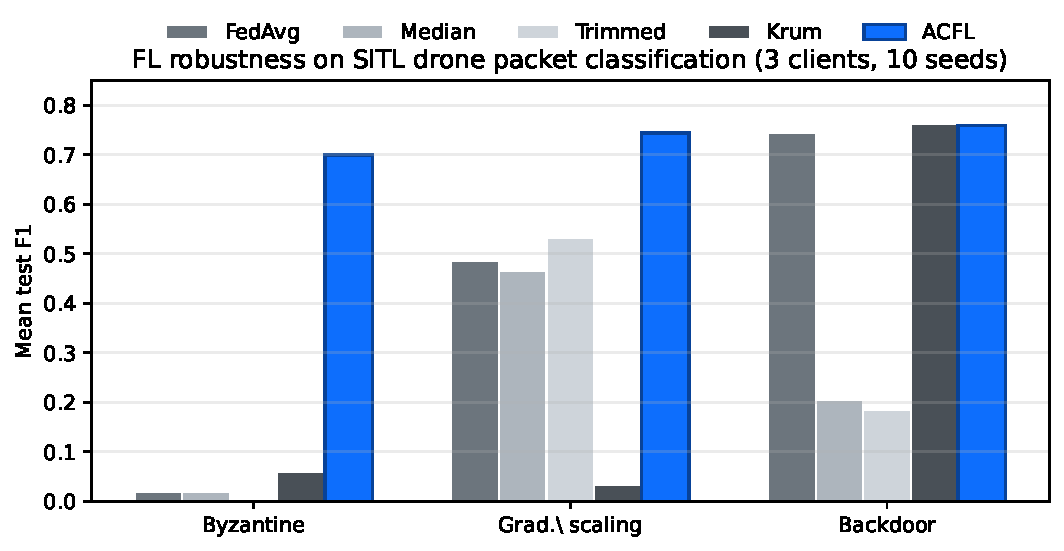
\includegraphics[width=\linewidth]{figures/fig_main_f1.pdf}
\caption{Mean test F1 across defenders and attacks on the SITL drone packet FL benchmark (3 clients, 12 rounds, 10 seeds). Only ACFL preserves utility under Byzantine attack; classical robust aggregators collapse or underperform FedAvg on gradient scaling and backdoor.}
\label{fig:main-f1}
\end{figure}

\begin{figure}[t]
\centering
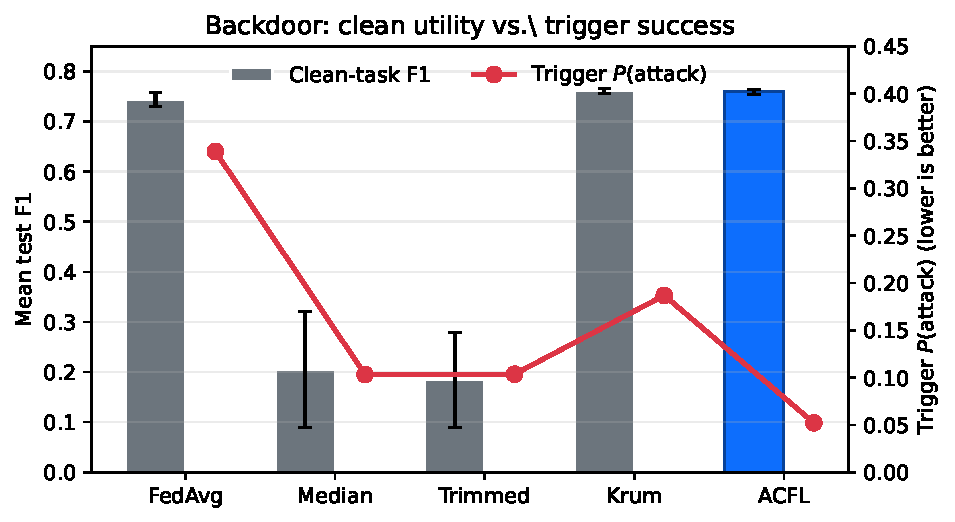
\includegraphics[width=\linewidth]{figures/fig_backdoor_dual.pdf}
\caption{Backdoor attack: clean-task F1 (bars, left axis) versus mean trigger $P(\text{attack})$ on counterfactual probes (line, right axis). Lower trigger probability indicates less successful backdoor activation. ACFL reduces trigger success relative to FedAvg and Krum while matching clean-task F1.}
\label{fig:backdoor-dual}
\end{figure}
.
